\documentclass[a4paper,11pt]{article}
\usepackage{jheppub}
\usepackage{graphicx}
\usepackage{amsmath}
\usepackage{amsfonts}
\usepackage{xspace}
\usepackage{hyperref}
\usepackage{placeins}
\usepackage{tikz}
\usepackage{tabularx}
\usepackage{multirow}
\usepackage{defs}
\usetikzlibrary{arrows.meta,positioning}
\setcounter{topnumber}{1}
\setcounter{bottomnumber}{1}
\setcounter{totalnumber}{2}
\renewcommand{\topfraction}{0.92}
\renewcommand{\bottomfraction}{0.45}
\renewcommand{\textfraction}{0.08}
\renewcommand{\floatpagefraction}{0.85}
\usepackage{lineno}
\linenumbers

% \title{Analysis note: LEP open data and precision physics as a testing ground for precision AI systems, an agentic measurement of thrust with ALEPH archived data}

% \title{LLM agents as experimental and theoretical physicists: a proof-of-concept measurement of thrust from LEP archived data}
% \title{Testing LLM Agents under Expert Supervision for Experimental Particle Physics using LEP Open Data} in Experimental Particle Physics with LEP Open Data: a proof of concept measurement }
\title{Agentic AI – Physicist Collaboration in Experimental Particle Physics: A Proof-of-Concept Measurement with LEP Open Data}

% Previous title candidates:
% Proof of concept measurement of LEP archived data with LLM AI agents
% LLM agents as experimental physicists: a proof-of-concept measurement of thrust from LEP archived data
% LEP open data and precision physics as a testing ground for precision AI systems, an agentic measurement of thrust with ALEPH archived data

\author[a]{Anthony Badea,}
\author[b]{Yen-Jie Lee,}
\author[c]{Marcello Maggi,}
\author[b]{Christopher McGinn,}
\author[d]{Austin Baty,}
\author[e]{Yi Chen,}
\author[b]{Hannah Bossi,}
\author[b]{Gian Michele Innocenti,}
\author[e]{Jingyu Zhang,}
\author[b]{Yu-Chen Chen,}
\author[b]{Tzu-An Sheng,}
\author[]{Electron-Positron Alliance}


\affiliation[a]{Enrico Fermi Institute, University of Chicago, Chicago, 60637 IL, USA}
\emailAdd{badea@uchicago.edu}
\affiliation[b]{Massachusetts Institute of Technology, Cambridge, MA 02139, USA}
\affiliation[c]{Istituto Nazionale di Fisica Nucleare, Bari Division, BA 70126, Italy}
\affiliation[d]{University of Illinois Chicago, Chicago, IL, USA}
\affiliation[e]{Vanderbilt University, Nashville, Tennessee, USA}%

\abstract{
We present an agentic measurement of the thrust distribution in $e^{+}e^{-}$ collisions at $\sqrt{s}=91.2$~GeV using ALEPH archived data.
This work was carried out through an AI agent–physicist collaboration, using interactive natural-language prompting of Anthropic Claude and OpenAI Codex. Under physicist guidance, the agents wrote and executed all analysis code and drafted the bulk of this paper.
A fully corrected thrust spectrum is obtained via Iterative Bayesian Unfolding and Monte Carlo based corrections. 
The principal contribution of this work is the demonstration of the agentic analysis, with thrust serving as a benchmark observable for the method. 
Dedicated precision measurements of thrust are reported in the community elsewhere. 
This work represents a step toward a theory--experiment loop in which AI agents assist with experimental measurements and theoretical calculations, and synthesize insights by comparing the results, thereby accelerating the cycle that drives discovery in fundamental physics.
Our work suggests that precision physics, leveraging the open LEP data and advanced theoretical landscape, provides an ideal testing ground for developing AI agent systems for scientific applications.
}

\keywords{quantum chromodynamics, AI agents, electron-positron collisions, event shapes}

\begin{document}
\maketitle

\section{Context of Electron-Positron Alliance}
\label{sec:context}

Modern collider datasets provide unprecedented statistical power, and experimental uncertainties on many Standard Model measurements are now at the percent level. In this regime, theoretical uncertainties increasingly limit the overall precision, and those associated with Quantum Chromodynamics (QCD) are among the dominant contributions. To achieve the physics goals of future programs, including the High-Luminosity LHC (HL-LHC) and Future Circular Collider (FCC-ee), theoretical predictions must therefore reach a precision comparable to the expected experimental uncertainties, in many cases at the sub-percent level, so that potential new physics anomalies can be interpreted reliably.

Precision QCD studies can be pursued at hadron colliders such as the LHC, but they are most cleanly and systematically tested in lepton collider environments. At present, however, there is no active high-energy lepton collider operating at Large Electron--Positron collider (LEP) energies or above. To address this, the Electron-Positron Alliance (EPA)~\cite{EEAlliance:website} works with LEP collaboration members to curated and reanalyze archived datasets, opening new opportunities enabled by three decades of theoretical advances and modern experimental techniques. The combination of ultra-precise $e^+e^-$ data and state-of-the-art perturbative and non-perturbative theory tools provides a uniquely powerful environment for high-precision studies. The EPA has produced a series of precision measurements using these archived datasets, including two-particle correlations~\cite{Badea:2019vey}, jet energy spectra and substructure~\cite{Chen:2021uws}, long-range near-side correlations at $WW$ threshold~\cite{Chen:2024lrc}, energy-energy correlators~\cite{Bossi:2025eec}, and unbinned measurement of thrust~\cite{Badea:2025ubt}.

More broadly, this program is a compelling opportunity for AI for Science in a domain where precision is paramount. While AI is increasingly used to assist theoretical calculations and generate predictions, in the physical sciences such predictions ultimately require experimental validation. In high-energy physics, this validation depends on collider datasets that are rarely publicly accessible. The $e^+e^-$ environment, particularly at LEP energies, provides the cleanest setting for precision tests of the Standard Model (SM), with well-defined initial states and calculable dynamics. The successful curation and use of archived open data therefore establishes the conditions for a theory--experiment loop in which AI systems, guided by domain experts, can propose new calculations, observables, or improved models and directly confront them with high-precision data. This creates a concrete framework for developing AI systems that do not merely interpolate existing knowledge, but actively refine theoretical descriptions through direct comparison with experiment. We believe that this technology is the start of an exciting scientific revolution.

\subsection*{Lessons from AI--Physicist Collaboration}

Carrying out this analysis has also produced practical insights into how AI agents and physicists can work together effectively. Our workflow followed a constrained human-in-the-loop cycle in which the physicist defined physics objectives, acceptance criteria, and interpretation authority, while the AI agent owned implementation and execution. Crucially, experienced physicists contribute domain context that cannot yet be reduced to formal specifications alone, including judgments about physically meaningful binning, acceptable regularization behavior, uncertainty communication, and when apparent anomalies warranted deeper investigation. A major future goal identified in this work is to translate this expert knowledge into explicit, code-based verification layers. 
%Requests were made concrete and executable, each iteration linked to specific scripts, outputs, and note sections, and corrections were applied incrementally rather than batched into large changes.

From this experience, several recurring challenge classes emerged. Implicit physics priors, expert expectations about acceptable binning, regularization behavior, or uncertainty presentation, were often assumed rather than explicitly stated, requiring iterative clarification. Figure formatting and style choices (label offsets, legend placement, pad geometry) required many short feedback loops, with cosmetic shortcomings sometimes affecting interpretability and therefore physics conclusions. Synchronization across rapidly evolving scripts, outputs, and note text demanded continuous provenance refreshing. These lessons motivate creation of reusable tools, stronger configuration contracts, clearer channels for encoding expert heuristics into machine readable constraints in future iterations of this program, and new verification layers throughout the autonomous analysis flow.
\section{Introduction}
\label{sec:introduction}

Machine learning has been central to high-energy physics for decades, enabling
reconstruction algorithms, event classification, and detector optimization across
collider experiments. A new frontier has emerged with large language models (LLMs)
developed by major AI laboratories, including
Anthropic~\cite{Anthropic:2025accelerating}, OpenAI~\cite{OpenAI:2025gpt5science},
Google DeepMind~\cite{GoogleDeepMind:2025geminiscience}, and others, that can now
assist directly with scientific reasoning, mathematical proof, and code generation.
A striking asymmetry persists: AI is transforming the theoretical and computational side of science research, assisting derivations of new results in theoretical particle physics~\cite{OpenAI:2025newresult}, designing novel protein structures for biology and health research~\cite{GoogleDeepMind:2025alphaproteo}, and simplifying complex calculations. Yet the experimental side of the AI-assisted research loop remains largely absent, especially in fundamental physics. To realize a future where AI rapidly accelerates the discovery of new physics, AI-assisted scientific workflows must be developed and validated across both theory and experiment.

A logical first step toward closing this gap is an agentic analysis of real
experimental data with expert physicist oversight. This is precisely the approach
pursued here. We communicated via natural language prompts with the Anthropic Claude and OpenAI Codex agents, brainstormed
analysis goals, then iteratively prompted the AI agents to execute the full
analysis workflow. No analysis code was written by hand. By analogy, the physicist's role is
similar to advising a graduate student, providing expert direction, reviewing
results, and iterating. The agent was supplied with context comprising the published ALEPH thrust paper~\cite{Heister:2003aj}, prior ROOT-based ALEPH analysis macros covering event selection and thrust calculation, internal analysis notes documenting the miniDST data format and detector calibration procedures, and the archived ALEPH data~\cite{ALEPH:docs}. This prompting strategy follows from our understanding in the AI literature that few-shot examples and supplied context improve AI-assisted outputs~\cite{Brown:2020fewshot,Wei:2022cot}. A detailed inventory of the inputs and prompting approach is given in Section~\ref{sec:ai_agent}.

This vision parallels the evolution of AI in neighboring scientific domains. In
materials science, chemistry, and biology, AI work has progressed from computational
prediction with post-hoc human validation toward AI-designed experiments executed
by autonomous robotic systems, creating closed feedback loops where AI proposes and orchestrates experiments and learns from them. High-energy physics faces a parallel opportunity, with exciting early progress for theory calculations~\cite{Abolhasani:2023sdl,MacLeod:2020sdl,Chen:2024scienceagentbench,Lu:2024aiscientist,Woodruff:2026practicalsi,Bubeck:2025coscientist,OpenAITheory:2026singleminus,Schwartz:2026cparameterllm}.
While we cannot deploy robots to construct particle experiments (yet), the emergence of open and curated data can serve as a
virtual laboratory for developing and validating AI-assisted scientific workflows
that operate across the precision theory--experiment
interface~\cite{Badea:2019vey,Chen:2021uws}.  This requires infrastructure on both sides: precise theoretical predictions and experimental measurements with rigorous uncertainty quantification, where AI-assisted reasoning is tested and held accountable to measurable constraints~\cite{Wang:2023aai,Messeri:2024aiu,Woodruff:2026practicalsi}.

Precision QCD is a natural domain for this program, because $e^{+}e^{-}$ annihilation offers both high-precision data and theory calculations. This matters because fine details are consequential: percent-level uncertainties, coupled to rigorous covariance estimates and end-to-end reproducibility, leave little room for an error to pass unnoticed. In hadronic or nuclear collision environments, by contrast, larger uncertainties can more easily conceal mistakes made by an AI system.

From both an AI and precision physics perspective, thrust is an ideal first observable for this program.
Thrust probes both perturbative radiation and non-perturbative dynamics in a
single distribution, is computable at high perturbative order, and has well-established
connections to resummed calculations, making comparison to theory controlled and
interpretable~\cite{PhysRevLett.39.1587,Abbate:2010xh,Heister:2003aj}. Thrust, along with other event-shape observables measured at LEP, continues to anchor comparisons between
perturbative calculations, generator modeling, and non-perturbative hadronization
constraints. Recent thrust-based $\alpha_s$ extractions report
$\alpha_s(m_Z)\simeq 0.1136\pm 0.0012$, below the 2023 world-average value
$\alpha_s(m_Z)=0.1180\pm 0.0009$~\cite{Benitez:2024nav,ParticleDataGroup:2022pth}.
This persistent tension, often referred to as the $e^{+}e^{-}$ $\alpha_{s}$ puzzle, is of great interest because $\alpha_{s}$ is the least precisely measured coupling constant of the Standard Model. The associated uncertainties propagate to all measurements involving QCD, and the effective field theory tools used to extract $\alpha_{s}$ are widely employed throughout the field. Put differently, if something is missed in the simplest case of $e^{+}e^{-}$ collisions, it is likely that similar effects will also be missed in precision studies of more complex systems. Therefore, testing the new AI technology on thrust in $e^+e^-$ collisions opens the door to significant progress in precision physics.

The objective of the agent-physicist collaboration in this work was to measure the thrust spectrum by applying appropriate selections, unfolding, corrections, and uncertainty handling. The agent was asked to execute the full analysis loop: data and simulation processing, unfolding orchestration,
systematic propagation, figure production, and note maintenance with traceable links
to code and outputs. We utilize the thrust measurement as a testing ground to understand the capabilities of the agents, establish a software base to conduct agentic analysis of the LEP data, and identify areas for improvement. We note that areas for improvement include both the core capabilities of the AI and the interaction of the physicist with the AI.
We envision using our work to pursue a next stage, where the same framework
will be extended to additional event-shape observables (C-parameter and heavy-jet
mass), and the approach of using AI-assisted scientific workflows for both theoretical
and experimental analysis will be pursued in a loop between them. 

The remainder of the document is structured as follows. Section~\ref{sec:ai_agent} defines the AI-agent operating model used in this work.
Section~\ref{sec:aleph} summarizes the ALEPH detector. Section~\ref{sec:datasets} describes data and simulation samples.
Section~\ref{sec:event_selection} details reconstruction and selections, including
particle-category and event-level validation. Section~\ref{sec:method} presents
thrust construction and the executable unfolding workflow.
Section~\ref{sec:systematics} discusses uncertainty measurements. Section~\ref{sec:results} presents the results of the measurement. Section~\ref{sec:conclusion} reports the conclusions from the study. 
%Section~\ref{sec:challenges} closes this work with persistent analysis challenges and mitigation tracking.

\section{AI-agent usage in this analysis program}
\label{sec:ai_agent}

This work includes an explicit evaluation of AI-agent support for an
experimental QCD analysis workflow. The central question is not only whether an
agent can generate text or isolated scripts, but whether it can execute a full
analysis loop under physicist supervision: data and Monte Carlo (MC) processing, unfolding
orchestration, systematic propagation, figure production, and note maintenance
with traceable links to code and outputs.

\subsection{Scope and operating model}

The agents used in this analysis are Anthropic Claude Code and OpenAI Codex, depending on the preference of the physicist.
The operating model is human-in-the-loop: the physicist formulates goals and
provides expert direction through iterative prompts; the agent executes the
corresponding implementation steps; the physicist reviews the outputs and
provides feedback; the process is then repeated. Physics decisions remain
analyst-owned, while the agent provides implementation speed, consistency
checks, and documentation rigor. In practical terms, the agent is used to:
\begin{itemize}
\item write, execute, and monitor analysis code,
\item enforce consistent plotting and note formatting conventions for work communication,
\item maintenance an understanding of which analysis code and configurations,
\item iterate quickly on ideas other time consuming tasks.
\end{itemize}

\noindent Our operating model is intentionally conservative to see how the agent performs when used to accelerate the common physics engineering and documentation tasks, rather than the core scientific decision tasks.

\subsection{Inputs and context supplied to agents}
\label{sec:agent_inputs}

The context supplied to the agent at the start of the session are the following.
\begin{itemize}
\item Context: the published ALEPH thrust measurement, prior ROOT-based analysis macros for event selection and thrust calculation, and internal analysis notes documenting the open data format, detector calibration, and object definitions~\cite{Heister:2003aj,ALEPH:docs}.
\item Datasets: the ALEPH LEP1 data files for the 1994 running period at $\sqrt{s}=91.2$~GeV, together with the corresponding ALEPH MC samples. Additional modern MC were given for theoretical uncertainty estimation.
\item Physicist-written prompts: prompts specifying the physics objective (e.g.\ ``propagate the hadronic-event correction as an independent systematic component with per-bin envelope uncertainties''), acceptance criteria (e.g.\ ``refolded spectra must reproduce detector-level data within statistical precision''), and output-format expectations (figure style, table layout, note section to update).
\end{itemize}

\subsection{Boundaries, controls, and reproducibility}

To keep scientific accountability explicit, each high-impact step has a control point where analyst sign-off is required before results are treated as baseline. The analysis stages where control points were used are: event and object selection definition, unfolding regularization choice, systematic-combination policy, final figure and uncertainty-presentation choices, interpretation description of the work. Beyond these sign-off gates, the physicist performed concrete validation checks at each major analysis stage by inspecting the artifacts of the agents work. These checks are enumerated here.

\begin{itemize}
    \item Event selection: Cut-flow yields were compared to the published ALEPH numbers~\cite{Heister:2003aj} to verify selection efficiency. Distributions of $\cos\theta_{\mathrm{thrust}}$ and $\varphi$ were inspected for detector artifacts; this step uncovered a localized $\varphi$ excess in the data that was traced to a detector region and checked before proceeding.
    \item Unfolding: Refolded spectra were required to reproduce the detector-level data within statistical precision. An iteration scan confirmed that the refolded-to-measured is stable as the regularization parameter is scanned.
    \item Systematic uncertainties: Each variation's impact on the unfolded distribution was inspected for large bin-to-bin fluctuations. The covariance and correlation matrices for individual components as well as the total were computed.
    \item Results: The unfolded thrust distribution was compared to the ALEPH\,2004 published result over the 42~reported bins. Per-bin uncertainty breakdowns and correlation matrices are reported.
    \item All figure captions, table entries, and interpretive statements in this work were reviewed by the physicist for physics accuracy. Agent-generated text was treated as a draft requiring human approval before inclusion in the baseline.
\end{itemize}

Reproducibility is ensured through multiple complementary mechanisms. All analysis steps are version-controlled, with code and configuration managed in a git repository so that any result can be traced to a specific commit and set of inputs. Workflow runs produce structured output artifacts, including summary files that capture the configuration used, the software versions, and caches of the exported spectra and covariance files. Physicist oversight at each review stage provides a layer of verification, with each step requiring explicit physicist approval before being promoted to the nominal result and the analysis to continue. These controls ensure that results are reproducible and that the physicist retains accountability for the scientific claims.

\section{ALEPH detector}
\label{sec:aleph}

ALEPH was a general-purpose LEP detector with near $4\pi$ coverage and high-precision charged-particle tracking in a 1.5~T solenoidal magnetic field~\cite{Decamp:1990jra,ALEPH:1994ayc}. The detector subsystems most relevant for this event-shape analysis are the central tracker, electromagnetic and hadronic calorimeters, and outer muon chambers.

The central tracking system combined a silicon vertex detector (VDET), an inner tracking chamber (ITC), and a large time projection chamber (TPC) with 21 pad rows covering $|\cos\theta|<0.97$. Together these detectors provided precise track parameters and momentum measurements, and they define the object-quality observables used in this analysis (for example $d_0$, $z_0$, and $N_{\mathrm{TPC}}$, defined in Sec.~\ref{sec:object_selection}). The single-track momentum resolution achieved by the combined tracking system is
$\sigma(1/p_T)\simeq 6\times10^{-4}$~GeV$^{-1}$ from the curvature measurement, to which a
multiple-scattering contribution must be added; it is negligible at high momentum and
dominates at low $p_T$. The corresponding constant terms for the calorimeter energy
resolutions below are likewise omitted here.
% NEEDS AUTHOR INPUT before submission: Referee 2 asks for the multiple-scattering term
% (they quote dpt/pt = 5e-3) and for the constant terms of the ECAL and HCAL energy
% resolutions. The full expressions are in Decamp:1990jra / ALEPH:1994ayc, both already
% cited above, but we have not read those papers and will not transcribe numbers we cannot
% check. Take the coefficients from the detector papers and state the complete expressions.
% Mirrored in referee/reviewer2.md.

The calorimeter system comprised two main subsystems. The electromagnetic calorimeter (ECAL) achieved an energy resolution of $\sigma_E/E \simeq 0.18/\sqrt{E\,[\mathrm{GeV}]}$, providing the primary response to photons and electromagnetic showers and anchoring the neutral-energy scale for event-shape reconstruction. The hadronic calorimeter (HCAL) with resolution $\sigma_E/E \simeq 0.85/\sqrt{E\,[\mathrm{GeV}]}$ is essential for neutral-hadron energy flow and global visible-energy reconstruction. The muon system outside HCAL supports lepton categorization in the archived ALEPH object definitions.

A key feature of the ALEPH reconstruction is the energy-flow algorithm, which combines tracking and calorimetric information to form a set of energy-flow objects that represent both charged and neutral particle candidates in the event. Tracking information dominates for charged particles, where the momentum resolution is superior to the calorimeter energy resolution. Calorimetric information provides the primary input for neutral particles (photons and neutral hadrons), which leave no track in the TPC. The combined energy-flow reconstruction achieves an energy resolution of $\sigma(E) = (0.59\pm0.03)\sqrt{E/\text{GeV}} + (0.6\pm0.3)$~GeV for hadronic events~\cite{Heister:2003aj}. This energy-flow approach, used in the ALEPH 2004 published event-shape analysis~\cite{Heister:2003aj}, is the particle-level input adopted for the present analysis. The 1998 ALEPH event-shape analysis~\cite{Barate:1996fi} used charged particles only to minimize model dependence on neutral-energy simulation; our nominal analysis follows the 2004 approach using both charged and neutral energy-flow objects, with a charged-only variation retained as a cross-check.

In this analysis, we use the archived ALEPH reconstructed object representation directly, including per-particle category labels (\texttt{pwflag}) and kinematic variables. Event-shape observables are built from selected charged and neutral energy-flow objects, so detector performance in each reconstructed particle category is a direct input to thrust migration and unfolding stability.

\section{Data and simulated event samples}
\label{sec:datasets}

The measurement uses archived ALEPH LEP1 data from 1994 at $\sqrt{s}\simeq 91.2$~GeV. This period is used because matched detector-level and generator-level archived MC inputs required for unfolding are available in this configuration. The 1994 sample corresponds to approximately 40~pb$^{-1}$ after quality requirements and provides the largest fully synchronized archived data/MC configuration for this workflow. Table~\ref{tab:sample_bookkeeping} summarizes the event counts in the nominal thrust workflow. The archived MC reco sample contains approximately 752k selected events compared to 1.33M in data. As a result of having fewer simulated events, MC statistical fluctuations are larger than those in data.

\begin{table}[ht!]
\centering
\begin{tabular}{l c c}
\hline
Sample & Total events & Selected events \\
\hline
1994 data reco & 1,365,440 & 1,326,376 \\
1994 MC reco & 771,597 & 751,878 \\
1994 MC gen (\texttt{tgen}) & 771,597 & 771,597 \\
1994 MC gen-before (\texttt{tgenBefore}) & 973,769 & 973,769 \\
\hline
\end{tabular}
\caption{Number of total and selected events in the archived data samples.}
\label{tab:sample_bookkeeping}
\end{table}

Detector corrections are derived from archived ALEPH MC processed through the same analysis chain. The archived \textsc{Pythia}~6~\cite{Sjostrand:2000wi} MC was produced with the standard ALEPH detector simulation software chain (\textsc{JETSET}~7.4 parton shower and hadronization with the ALEPH tune, \textsc{GEANT}~3 detector simulation), consistent with the simulation used in the published ALEPH event-shape analyses of the same dataset~\cite{Heister:2003aj}. In the archived sample, the detector-level and generator-level event records are connected through a common event identifier, enabling event-matched response construction and post-unfolding hadronic-selection corrections. 

The unfolding step consumes four synchronized inputs, each a ROOT \texttt{TTree} in the
archived sample: measured data tree (\texttt{t}), detector-level MC tree (\texttt{t}), generator-level MC tree used for response matching (\texttt{tgen}), generator-level MC tree before hadronic event selection (\texttt{tgenBefore}). The ratio \texttt{tgenBefore/tgen} is used to derive a hadronic event-selection correction applied after unfolding. Event matching between reco and gen levels is performed with the unique event identifier. To populate the response matrix for unfolding, generator entries are matched to the reconstructed selected-event identifier set, consistent with the matched-response construction described in Sec.~\ref{sec:method}.

In addition to the archived baseline MC, alternative modern generator predictions from \textsc{Pythia}~8.317, \textsc{Herwig}~7.1.5, and \textsc{Sherpa}~2.2.6 are used in this work through event-level reweighting variations to estimate theory model dependence. These variations are propagated as dedicated systematic components in the final uncertainty model while preserving the same detector-response baseline.

\section{Event reconstruction and selection}
\label{sec:event_selection}

% This section describes particle selection, hadronic event definition, and particle-category data/MC validation before unfolding. This validation is essential because the selected particles are the direct inputs to the thrust algorithm.

\subsection{Object definitions}
\label{sec:particle_categories}

The archived reconstruction builds energy-flow candidates from combined
tracking and calorimeter information. Charged particle candidates rely on high-quality tracking
measurements, while neutral particle candidates utilize the calorimeter. The objects are categorized with an integer label \texttt{pwflag} as summarized in Table~\ref{tab:pwflag_definition}.

\begin{table}[ht!]
\centering
\begin{tabular}{c l}
\hline
\texttt{pwflag} & Category \\
\hline
0 & charged hadrons \\
1 & electrons (tracker + ECAL category) \\
2 & muons (tracker + muon category) \\
3 & $V^{0}$ candidates \\
4 & photons \\
5 & neutral hadrons \\
\hline
\end{tabular}
\caption{Object labels used in archived ALEPH events.}
\label{tab:pwflag_definition}
\end{table}

\noindent $V^0$ candidates (\texttt{pwflag}=3) include $K_S$ and $\Lambda$ from displaced-vertex reconstruction. These objects enter the thrust sum with their measured momentum vector rather than individual decay products, which is consistent with treating them as single hadronic objects for event-shape purposes. Their contribution to the thrust numerator and denominator is captured by the neutral-response systematic variations.

\subsection{Object and event selections}
\label{sec:object_selection}

Table~\ref{tab:particle_selection_summary} lists the object-level selection. These criteria define which reconstructed objects are propagated into thrust and therefore which detector effects enter the response model. They are imposed on the reconstructed collection only; the generator-level particles of the same events are retained without them. Here $d_0$ and $z_0$ are the transverse and longitudinal impact parameters of the track with respect to the per-event reconstructed primary vertex. Both are taken from the archived reconstruction. $N_{\mathrm{TPC}}$ is the number of TPC coordinates associated with the track.

\begin{table}[ht!]
\centering
\begin{tabular}{@{}p{0.37\textwidth}p{0.57\textwidth}@{}}
\hline
Object variable & Requirement \\
\hline
Charged category & \texttt{pwflag}\,$\in[0,2]$ \\
Charged acceptance & $|\cos\theta|\le 0.94$ \\
Charged transverse momentum & $p_{\mathrm{T}}\ge 0.2$ GeV \\
Charged impact parameter & $|d_0|\le 2$ cm \\
Charged longitudinal impact & $|z_0|\le 10$ cm \\
Charged hit quality & $N_{\mathrm{TPC}}\ge 4$ \\
Neutral category & \texttt{pwflag}\,$\in[3,5]$ \\
Neutral energy & $E\ge 0.4$ GeV \\
Neutral acceptance & $|\cos\theta|\le 0.98$ \\
Use charged objects & \texttt{keepChargedTracks} = \texttt{True} \\
Use neutral objects & \texttt{keepNeutralTracks} = \texttt{True} \\
\hline
\end{tabular}
\caption{Object selections applied to data and detector level MC.}
\label{tab:particle_selection_summary}
\end{table}

The hadronic event selection is summarized in Table~\ref{tab:event_selection_summary}, following the standard ALEPH selection~\cite{Heister:2003aj, Barate:1996fi}. These selections enforce a phase space with high tracking quality, controlled forward acceptance, and stable visible-energy topology before entering event-shape reconstruction. The residual contamination from $e^+e^- \rightarrow \tau^+\tau^-$ processes such as is expected to be less than 0.26\% for these event selections~\cite{Barate:1996fi}. Approximately 1.36 (1.32) million $e^+e^-$ collisions resulting in the decay of a Z boson to quarks are analyzed (selected). Note that the acceptance requirement based on the event shape variable sphericity introduces a slight sculpting of the thrust distribution. The cut removes approximately 2.3\% of selected events, with the largest effect in the multijet region. In data, the ratio of the thrust distribution with the cut to that without rises monotonically from $\approx 0.85$ at $T \approx 0.6$--$0.75$ to $\approx 0.95$ at $T \approx 0.9$ and $\approx 0.99$ as $T \to 1$.

\begin{table}[ht!]
\centering
\begin{tabular}{@{}p{0.37\textwidth}p{0.57\textwidth}@{}}
\hline
Event variable & Requirement \\
\hline
% Ntuple preselection & \texttt{passesNTupleAfterCut} = 1 \\
Total charged energy & $E_{\mathrm{trk}}^{\mathrm{tot}}\ge 15$ GeV \\
Sphericity-axis acceptance & $|\cos\theta_{\mathrm{Sph}}|\le 0.82$ \\
Charged multiplicity & $N_{\mathrm{trk}}\ge 5$ \\
Total multiplicity & $N_{\mathrm{trk}}+N_{\mathrm{neu}}\ge 13$ \\
\hline
\end{tabular}
\caption{Nominal event selections applied to data and detector level MC to build the nominal thrust input particle set.}
\label{tab:event_selection_summary}
\end{table}

% An earlier iteration of this analysis rejected \texttt{pwflag}=5 objects in $-0.19\le\cos\theta<-0.18$, a narrow window corresponding where a detector level enhancement in the particle yield is observed but not fully understood. This yield has negligible effect on the thrust measurement and is covered within a systematic variation affecting the neutral particle acceptance.

\subsection{Data-MC kinematic checks}

Before constructing thrust-family observables, we validate the reconstructed particle-level
ingredients that enter the event-shape sums and axis determination. Any mismodeling in particle
acceptance, momentum scale, or category composition can propagate into migration in the detector response matrix and into unfolded distributions. To assess detector modeling of these inputs, we compare data and MC reco distributions for each object category using Data/MC ratio panels, with generator-level references.

The charged-track category is shown in Fig.~\ref{fig:pwflag0_full}. Data/MC agreement is good in the bulk of all distributions. The $\cos\theta$ panel shows the geometric acceptance
cutoff at $|\cos\theta|=0.94$, with consistent data/MC behavior across the accepted
range. The impact-parameter panels ($d_0$, $z_0$) show the effect of the nominal
selection quality cuts, with both data and MC reproducing the expected Gaussian core
and non-Gaussian tails. The $N_{\mathrm{TPC}}$ distribution, a detector hit count rather than a generator observable, is well reproduced by the simulation. The measured momentum is translated to energy through the pion mass assumption.

Figure~\ref{fig:pwflag1_full} shows the electron objects. Relative to
charged tracks, this category has smaller yields and larger statistical fluctuations, but the
detector-level and MC shapes remain consistent across the main selection observables. The
comparison is important because isolated energetic leptons can rotate the thrust axis in otherwise two-jet-like events and can therefore influence migration in specific bins. Figure~\ref{fig:pwflag2_full} shows the muon object candidates, providing a direct
cross-check of category-dependent acceptance and momentum-shape modeling. This category probes
objects that utilize the muon subdetectors, so agreement here confirms that lepton-category partitioning does not induce a hidden detector asymmetry in the thrust inputs.

Figure~\ref{fig:pwflag3_full} shows $V^0$ candidates from displaced-vertex reconstruction. These enter the thrust sum as single four-vectors. Data/MC agreement in the bulk $\cos\theta$ and energy distributions is adequate. Data/MC differences are more visible than for charged tracks. Figure~\ref{fig:pwflag4_full} shows the photon category reconstructed by the ECAL. Data/MC agreement is generally good in the central region. Some modulations of the generator-level $\phi$ spectrum are seen which have a negligible impact on the result and are believed to be an artifact of how photons were stored in the sample. Figure~\ref{fig:pwflag5_full} shows the neutral hadronic calorimeter objects. Data/MC differences are largest in this category, in the neutral hadronic energy range of a few GeV. These differences are propagated through the dedicated neutral-response systematic branches and do not affect the nominal response matrix.

Event-level variables used for hadronic selection are also validated with data/MC comparisons, as shown in Fig.~\ref{fig:event_selection_observables}. These observables summarize the selected particle content and accepted topology that define the phase space used to build detector response and unfolded event-shape spectra.

\begin{figure}[ht!]
\centering
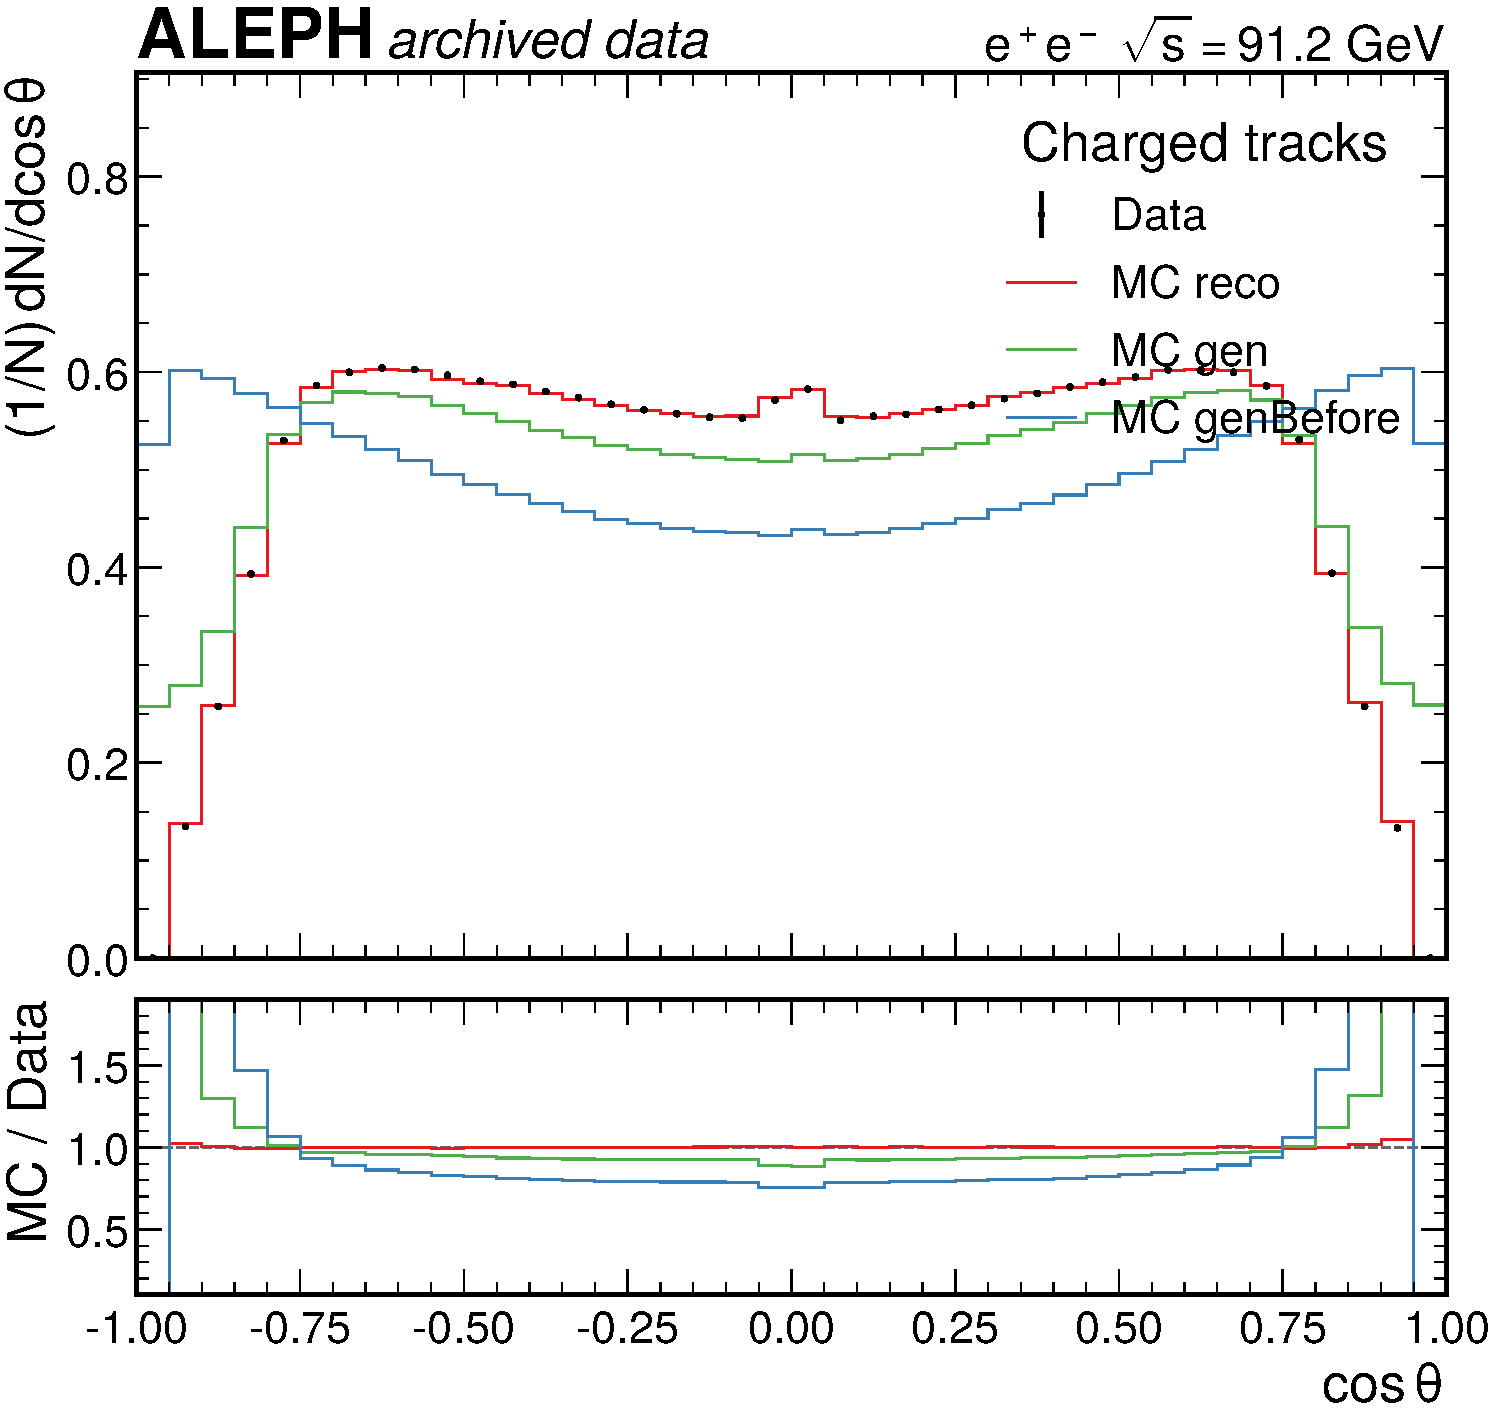
\includegraphics[width=0.242\textwidth]{figures/pwflag0_cosTheta.pdf}
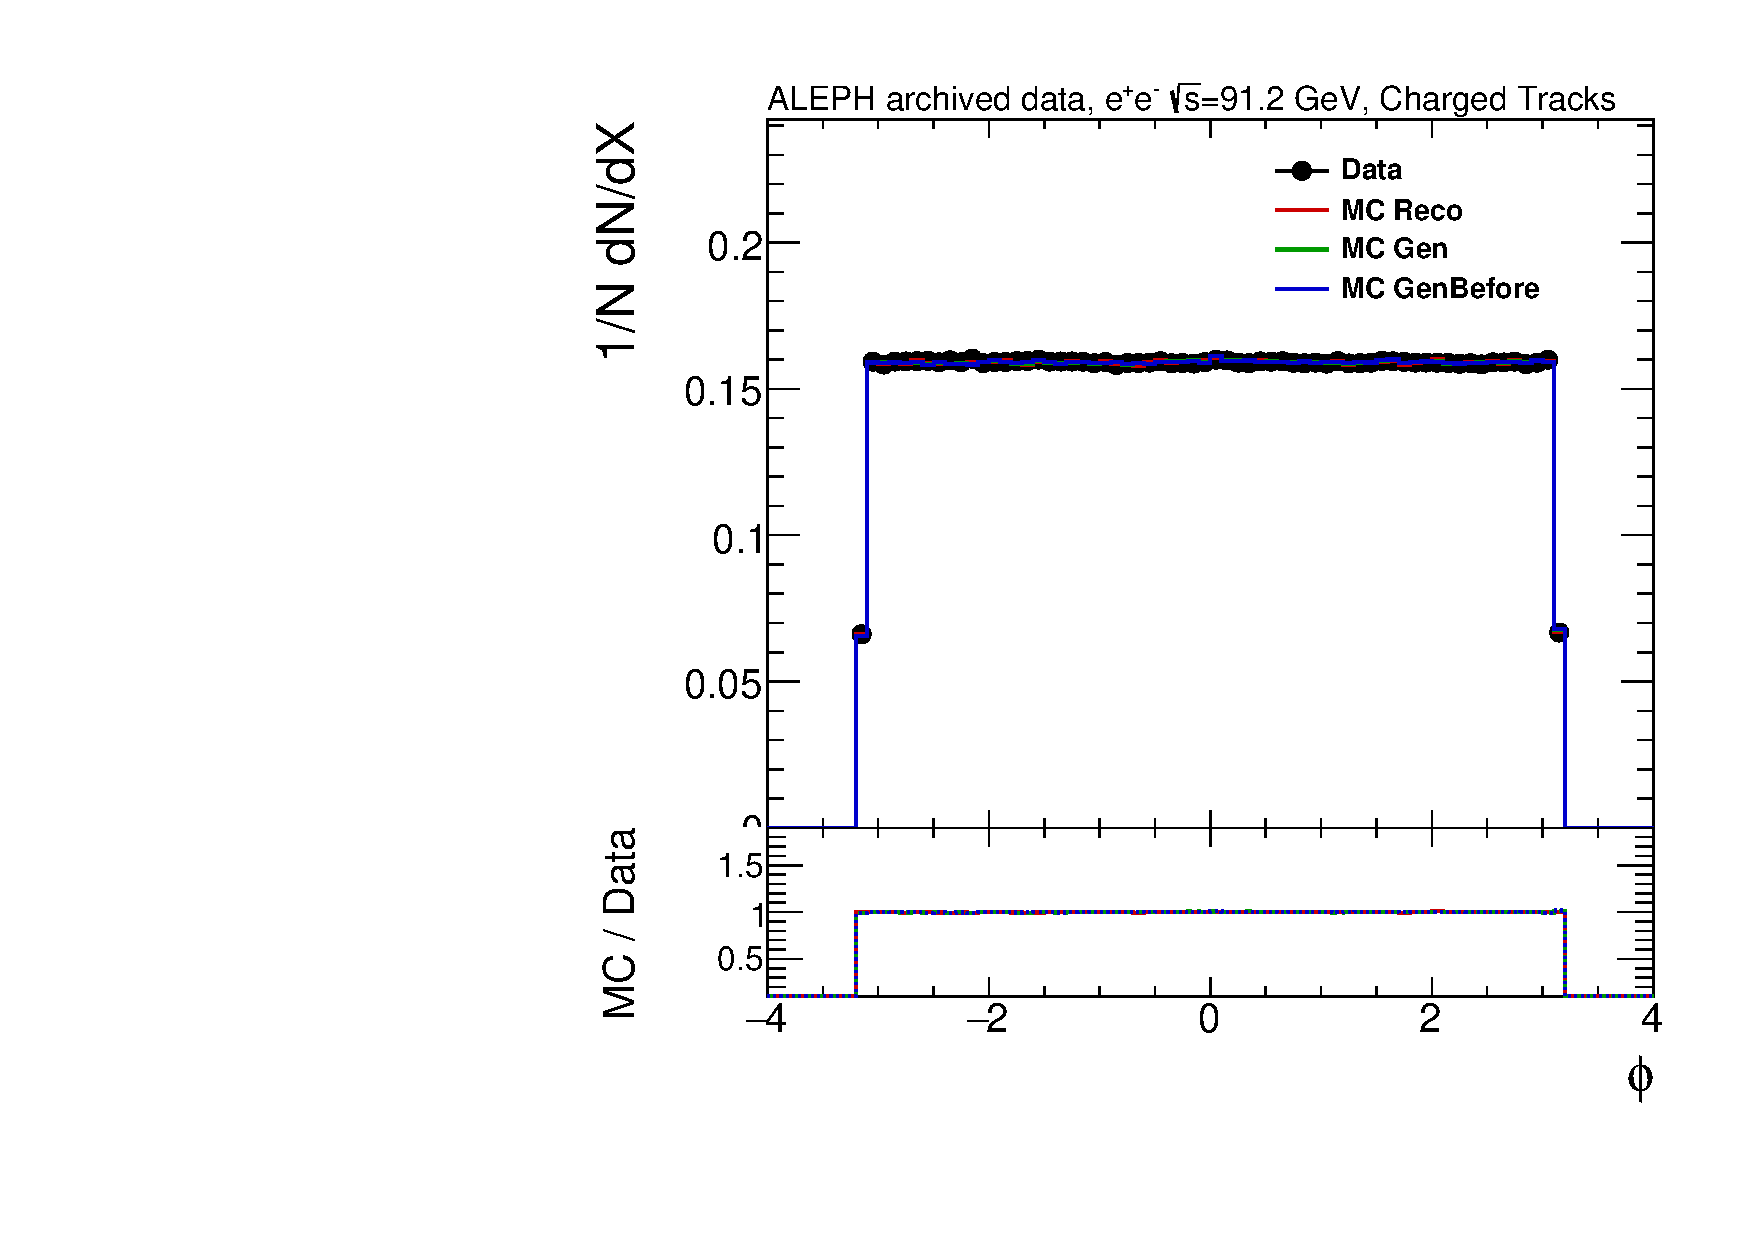
\includegraphics[width=0.242\textwidth]{figures/pwflag0_phi.pdf}
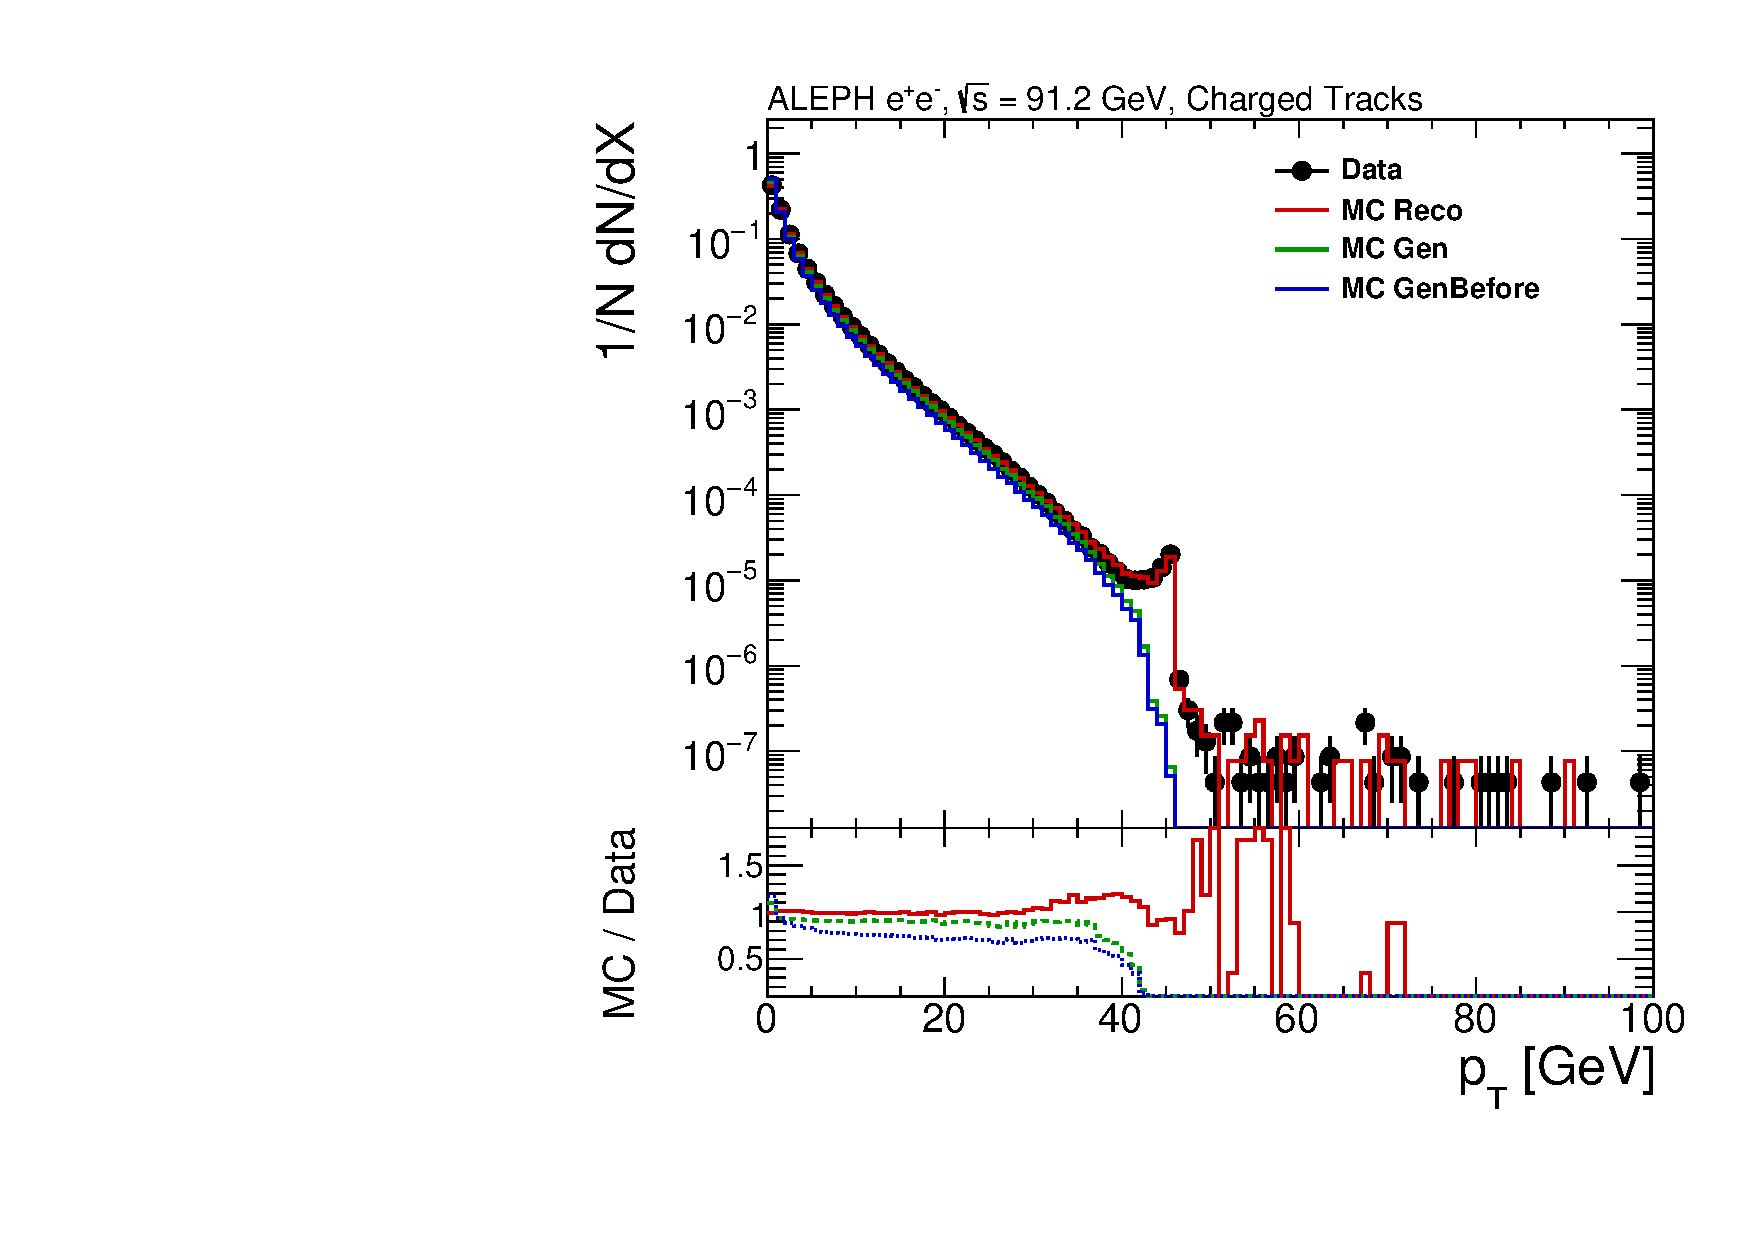
\includegraphics[width=0.242\textwidth]{figures/pwflag0_pt.pdf}
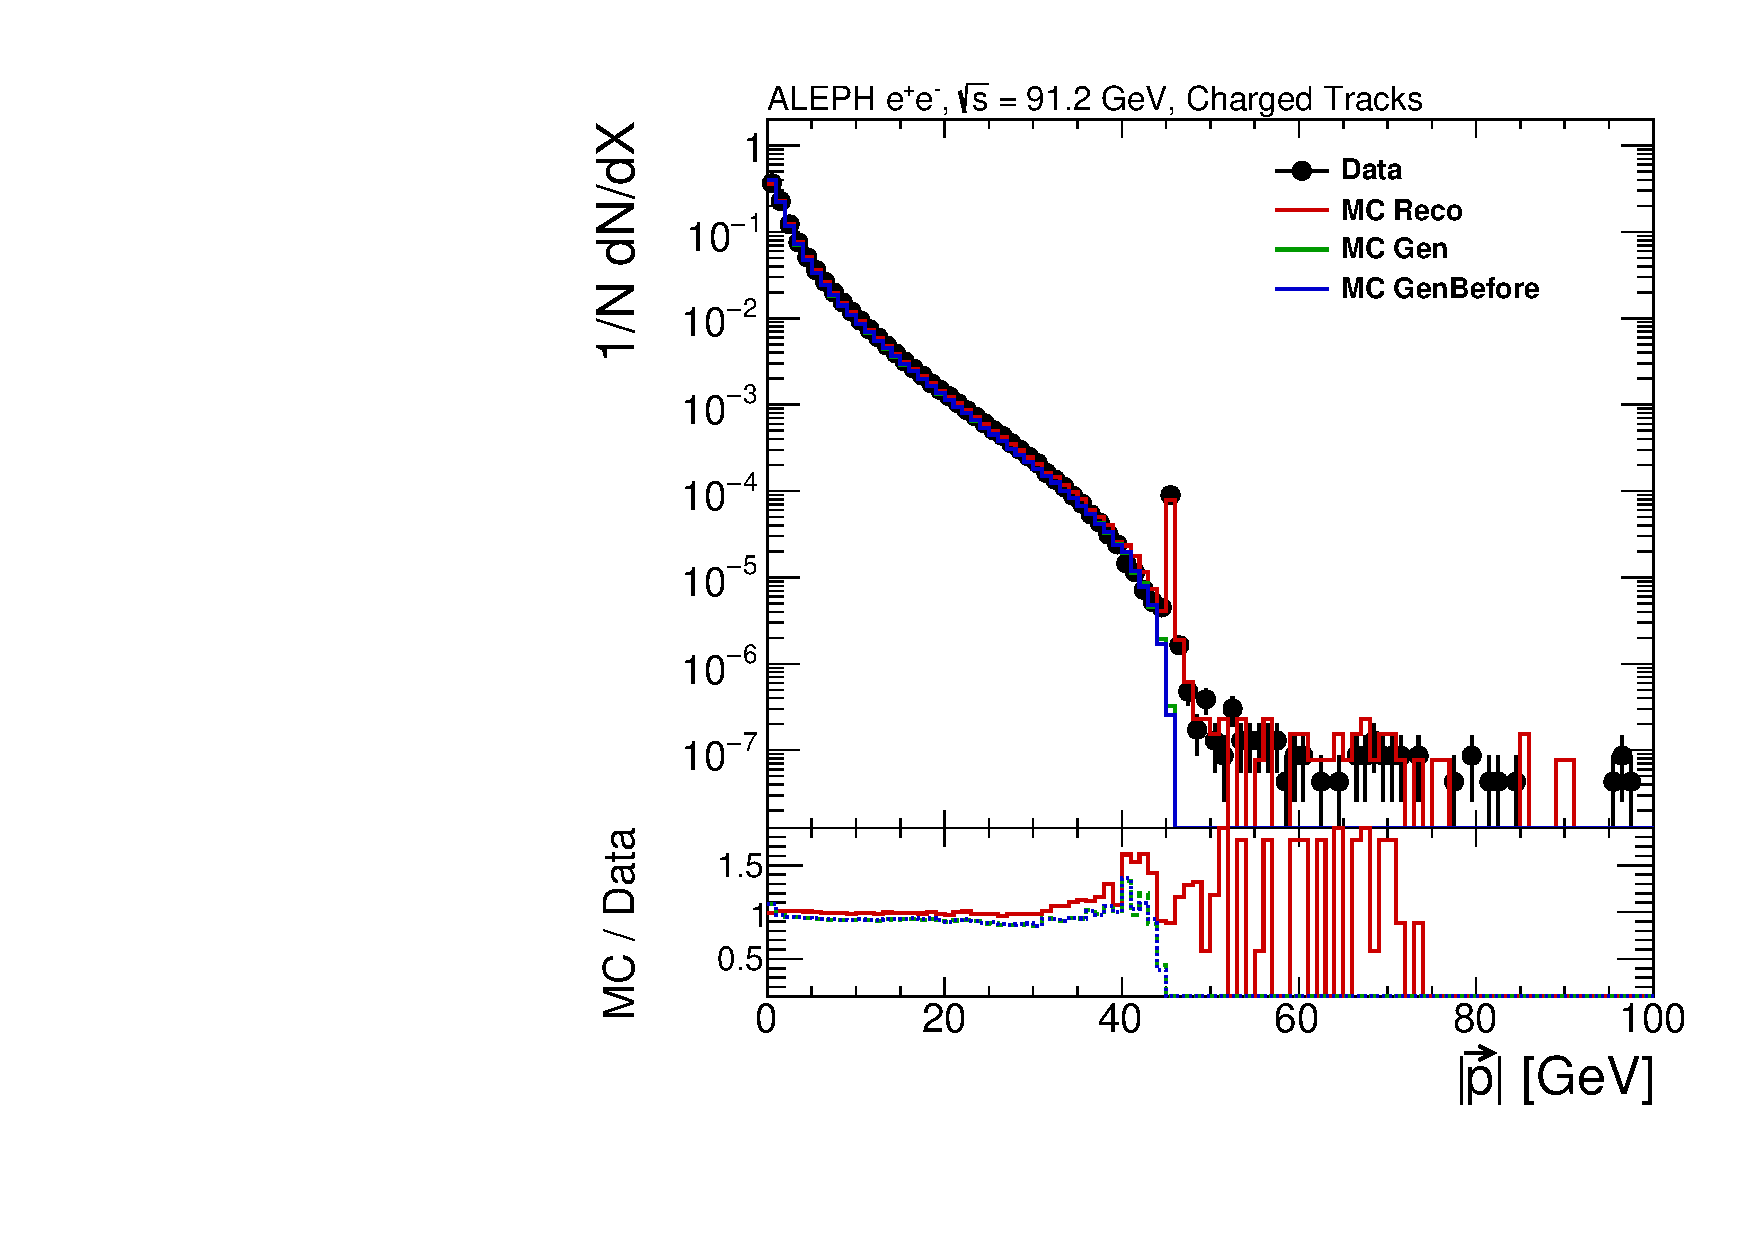
\includegraphics[width=0.242\textwidth]{figures/pwflag0_pmag.pdf}
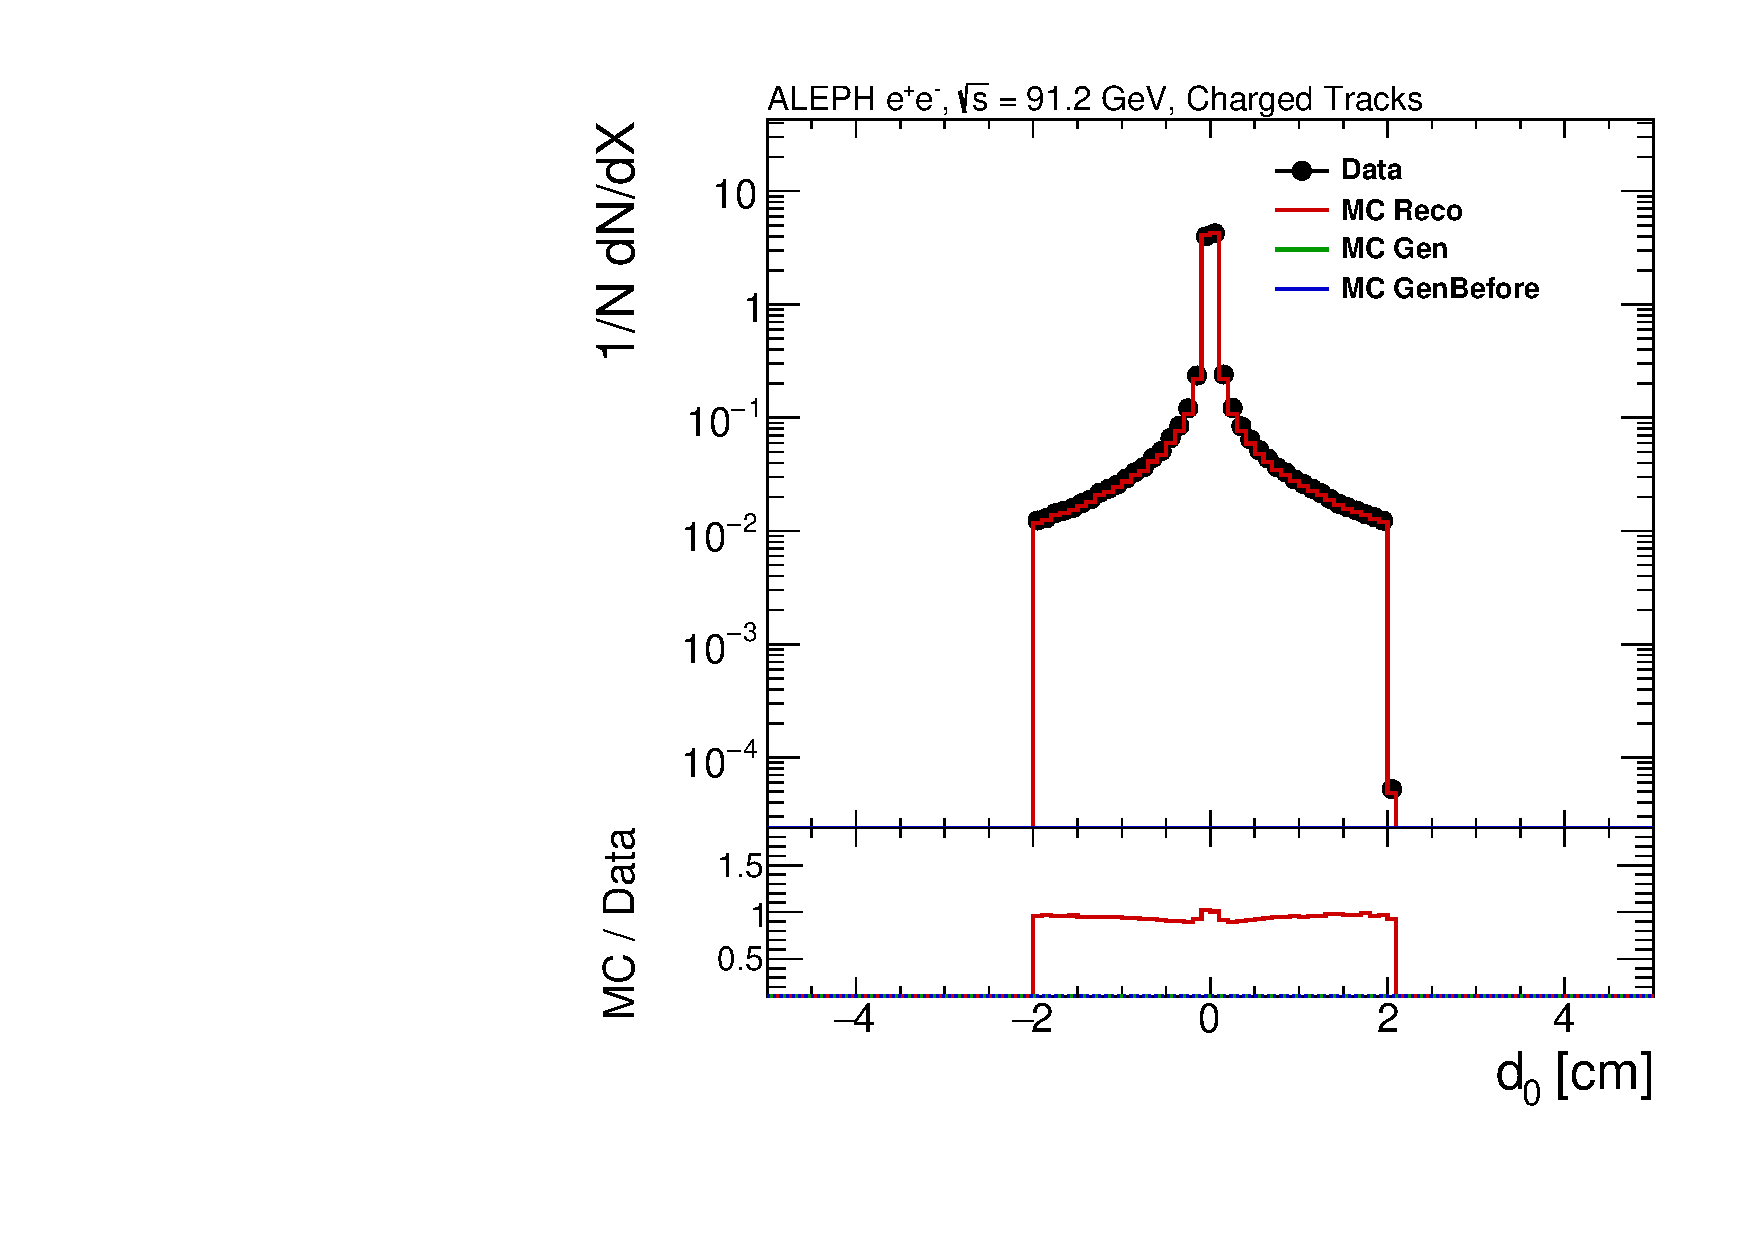
\includegraphics[width=0.242\textwidth]{figures/pwflag0_d0.pdf}
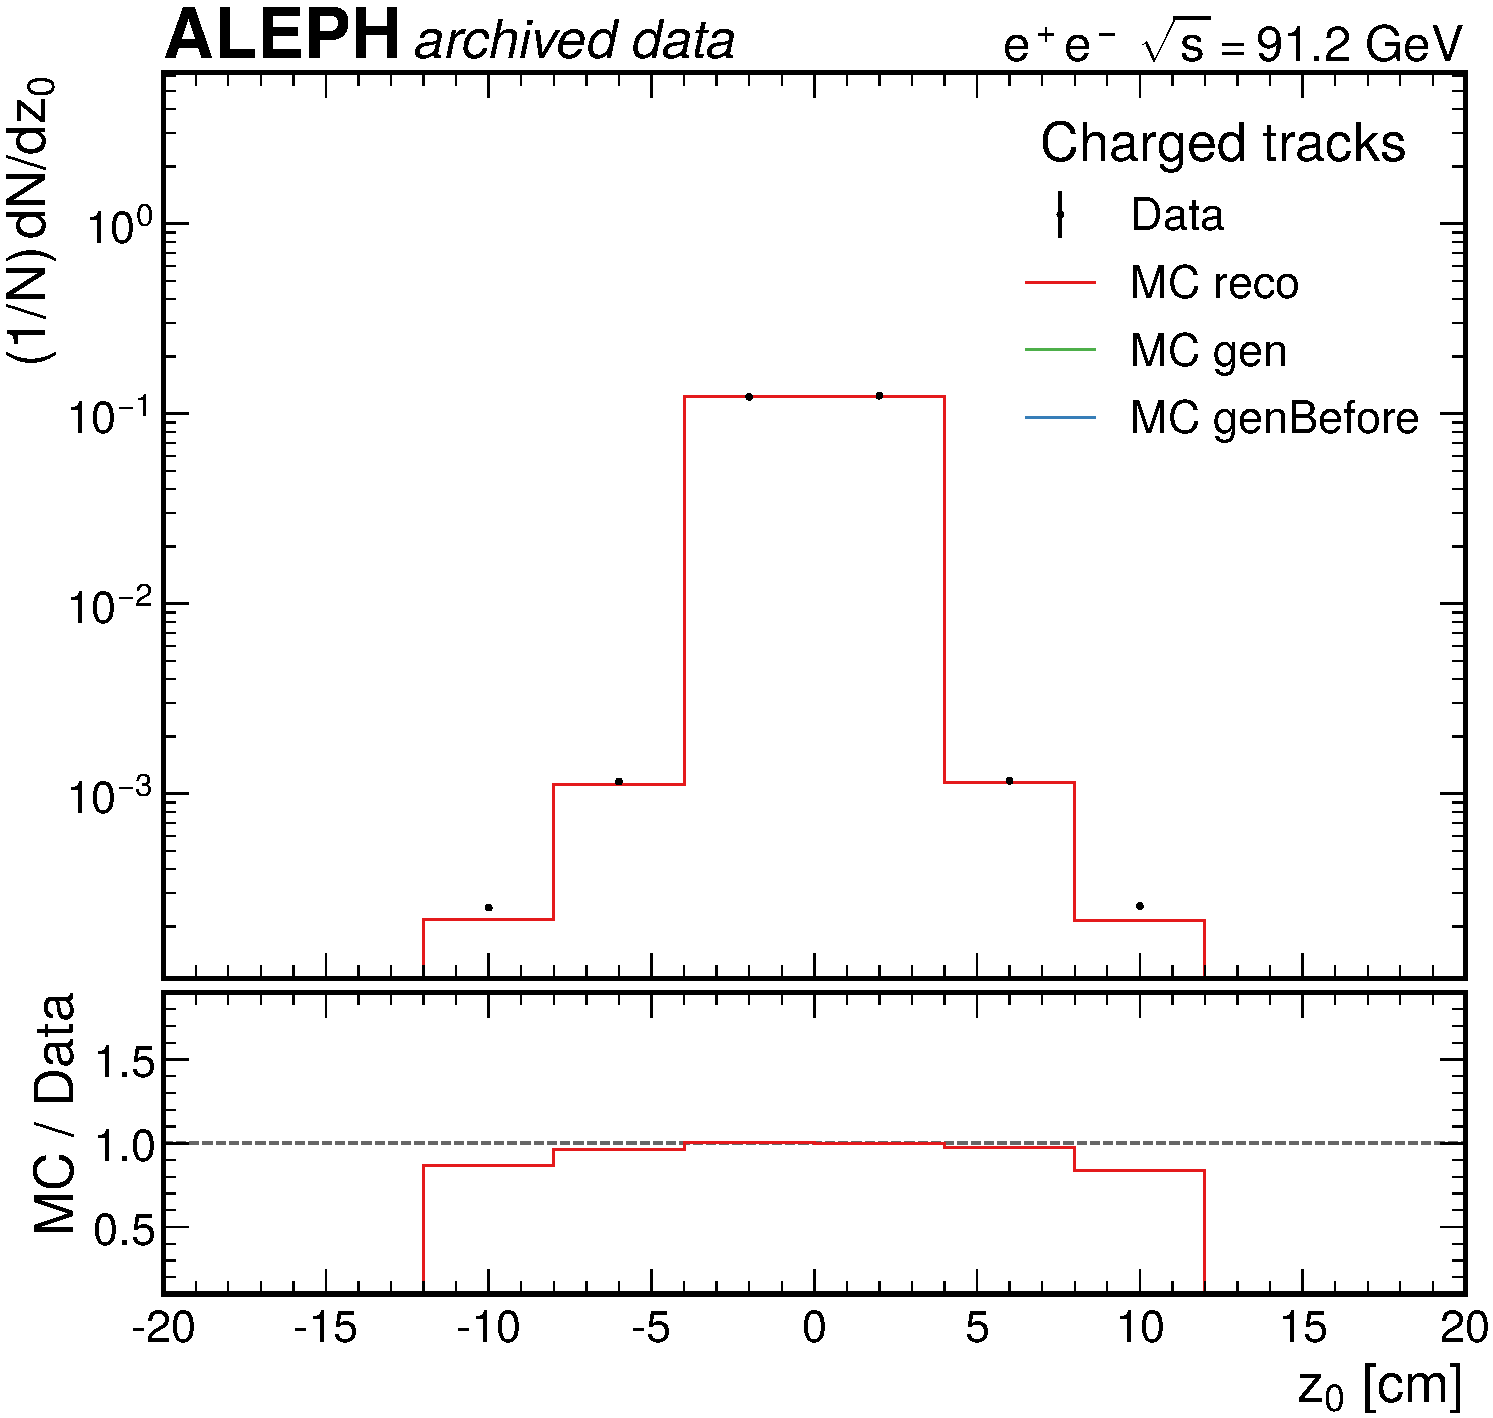
\includegraphics[width=0.242\textwidth]{figures/pwflag0_z0.pdf}
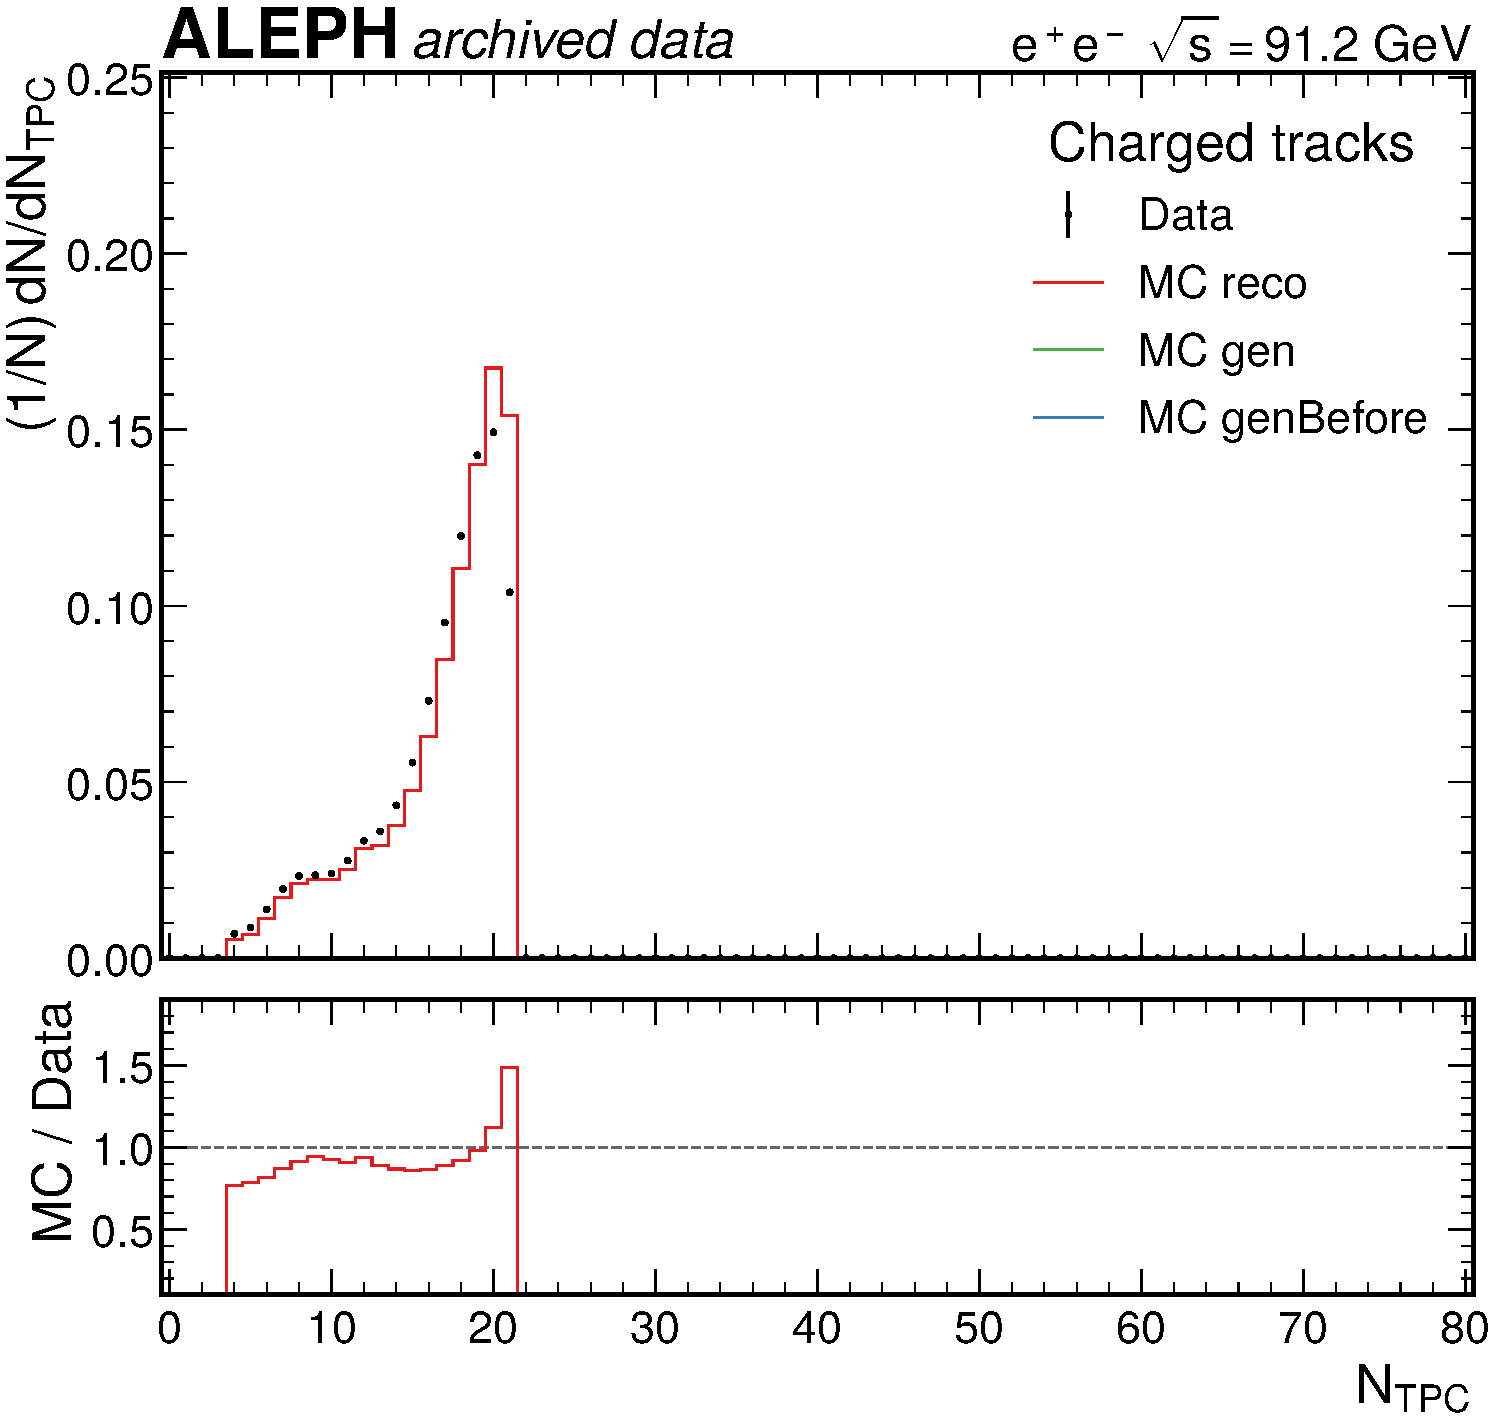
\includegraphics[width=0.242\textwidth]{figures/pwflag0_ntpc.pdf}
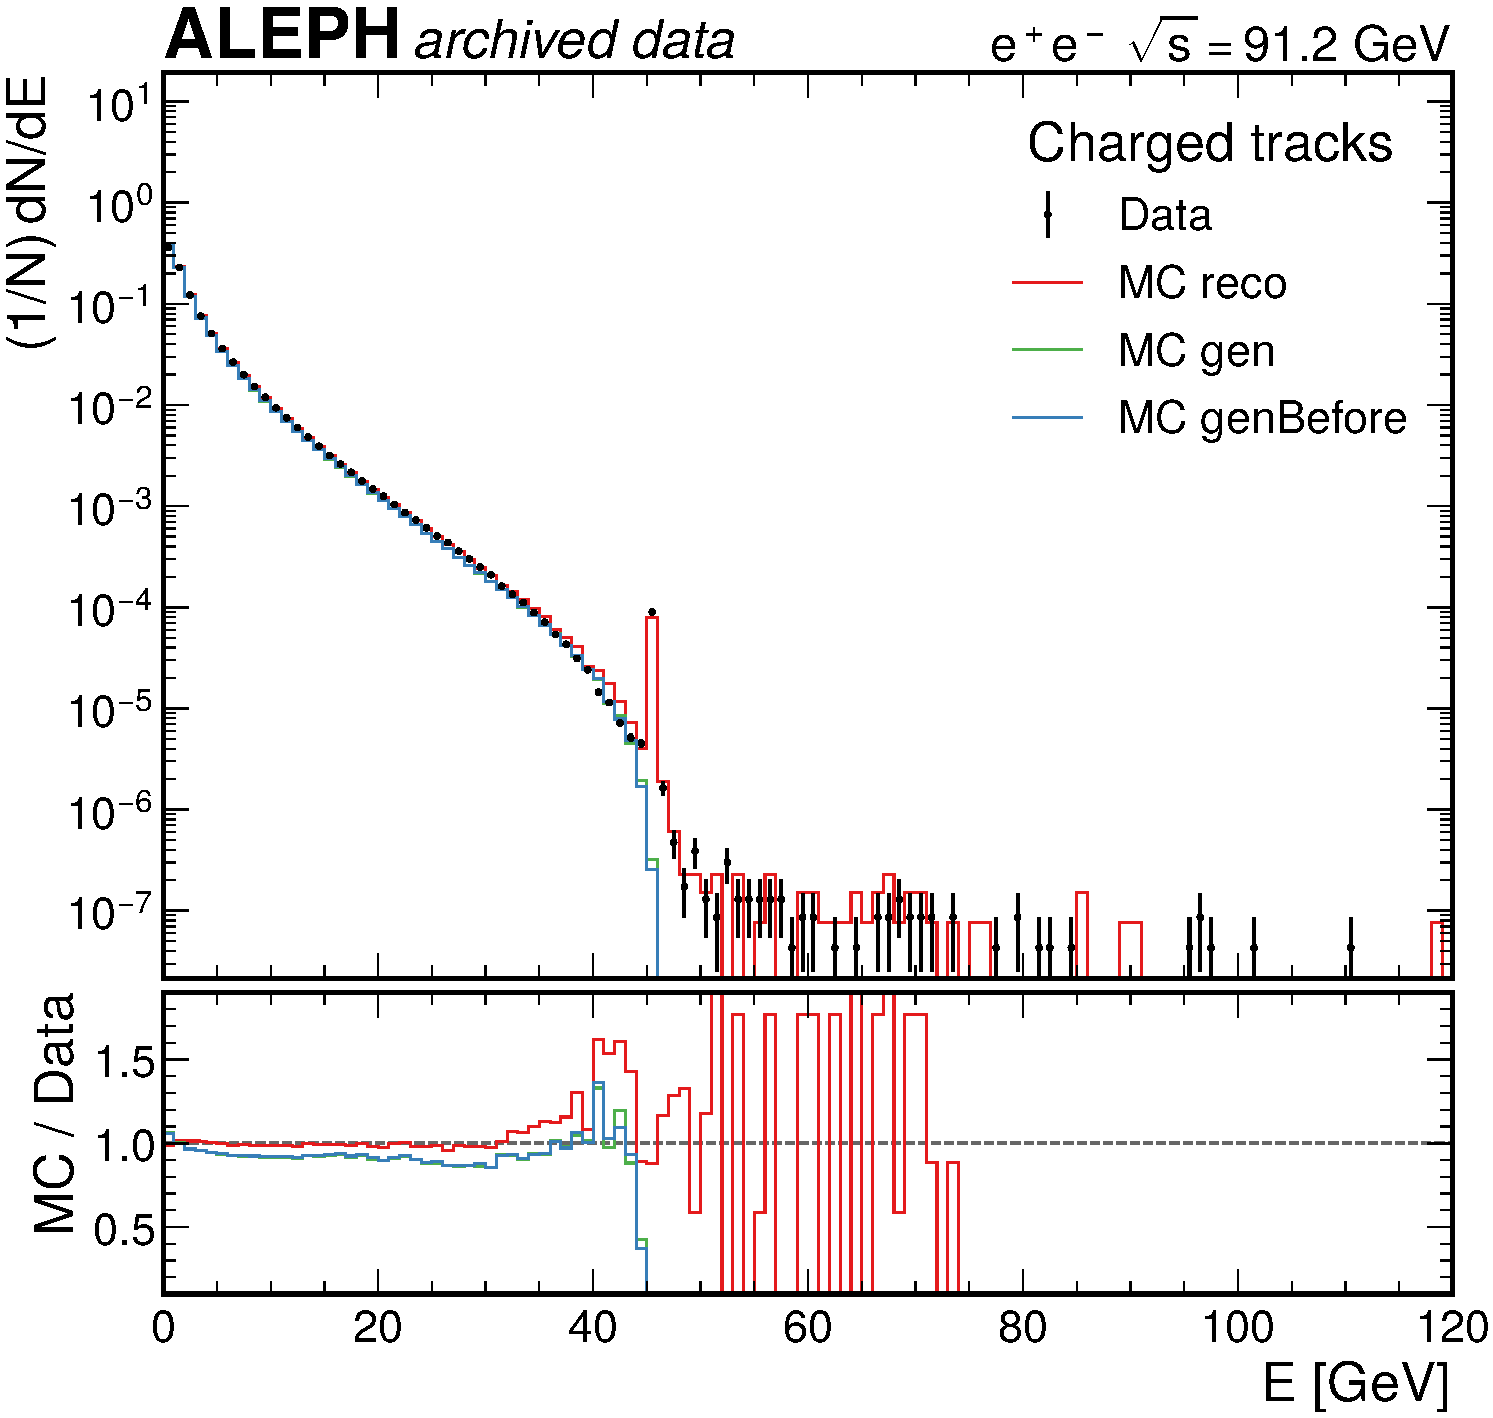
\includegraphics[width=0.242\textwidth]{figures/pwflag0_energy.pdf}
% 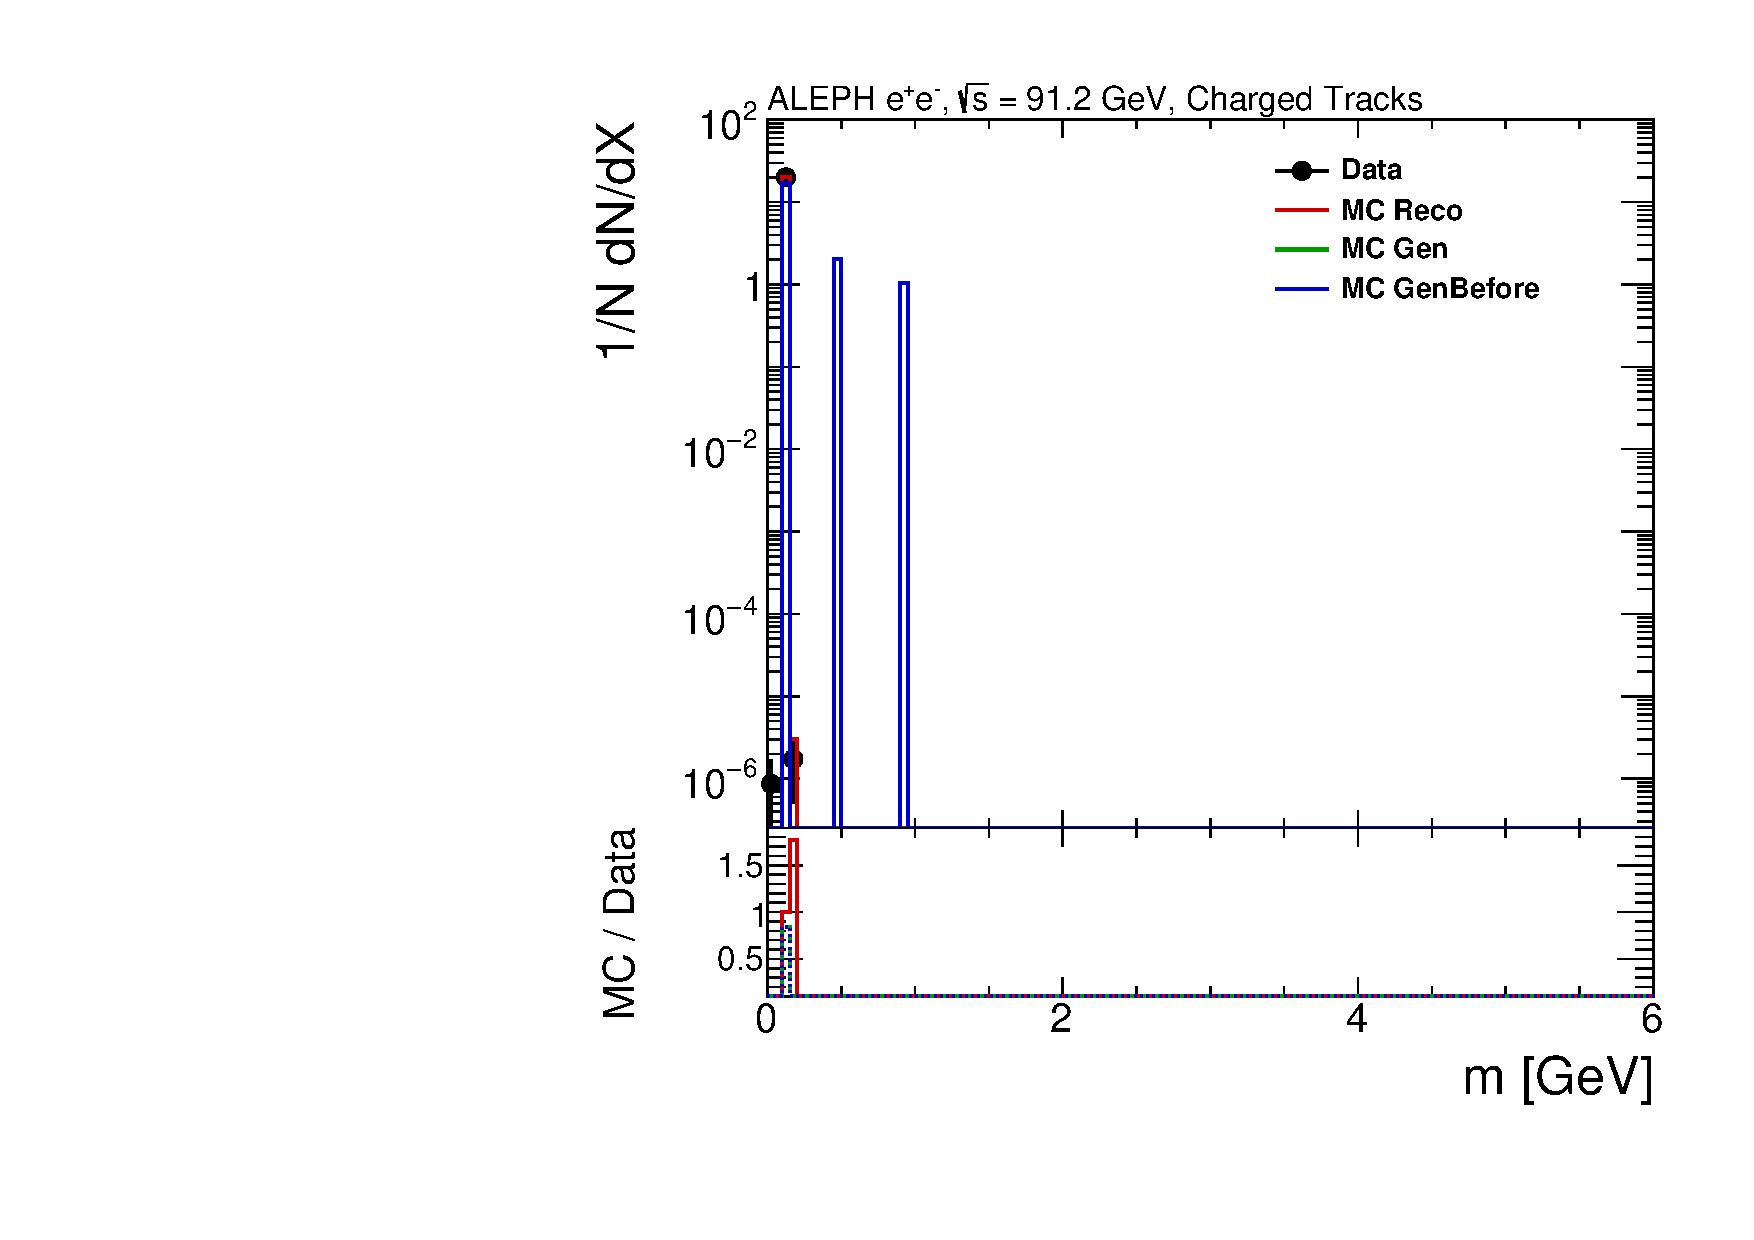
\includegraphics[width=0.242\textwidth]{figures/pwflag0_mass.pdf}
\caption{Complete \texttt{pwflag}=0 kinematic set.}
\label{fig:pwflag0_full}
\end{figure}

\begin{figure}[t!]
\centering
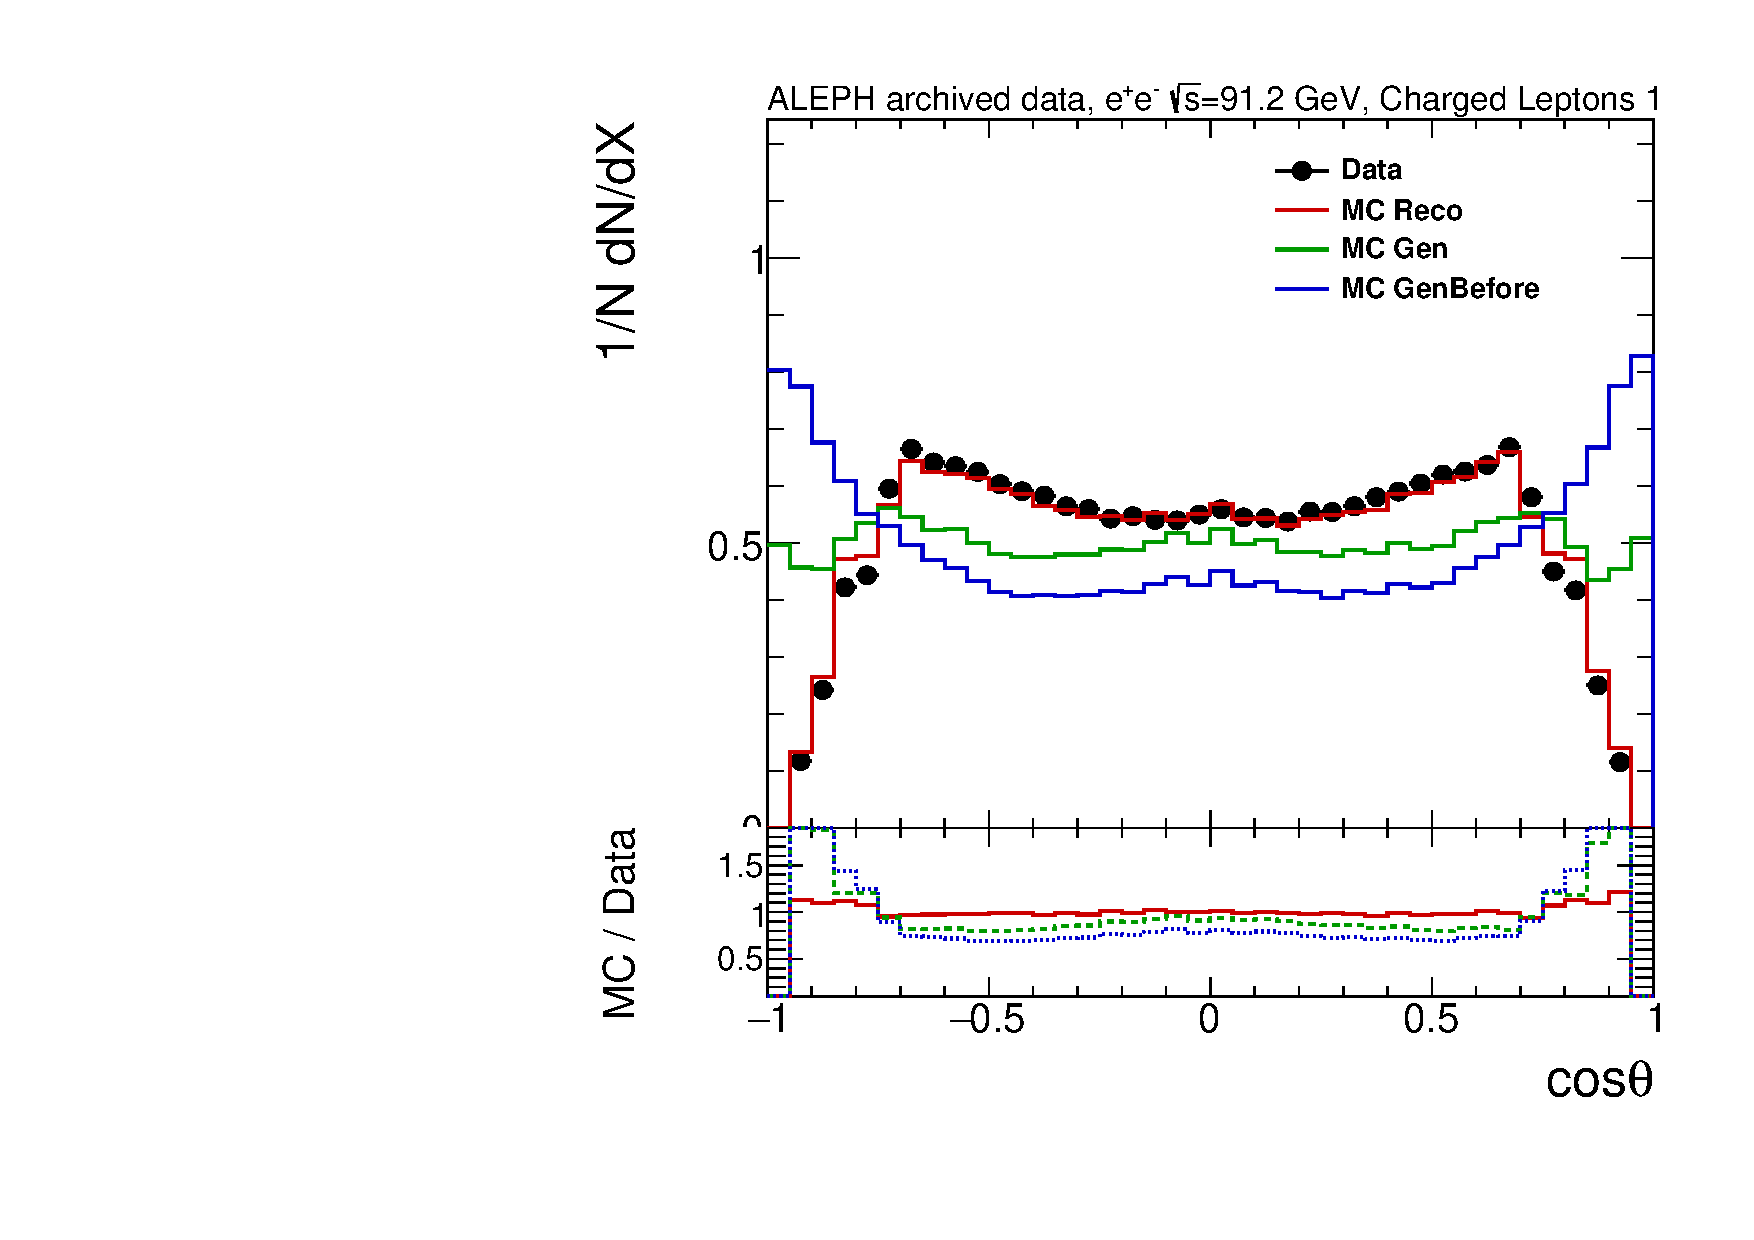
\includegraphics[width=0.242\textwidth]{figures/pwflag1_cosTheta.pdf}
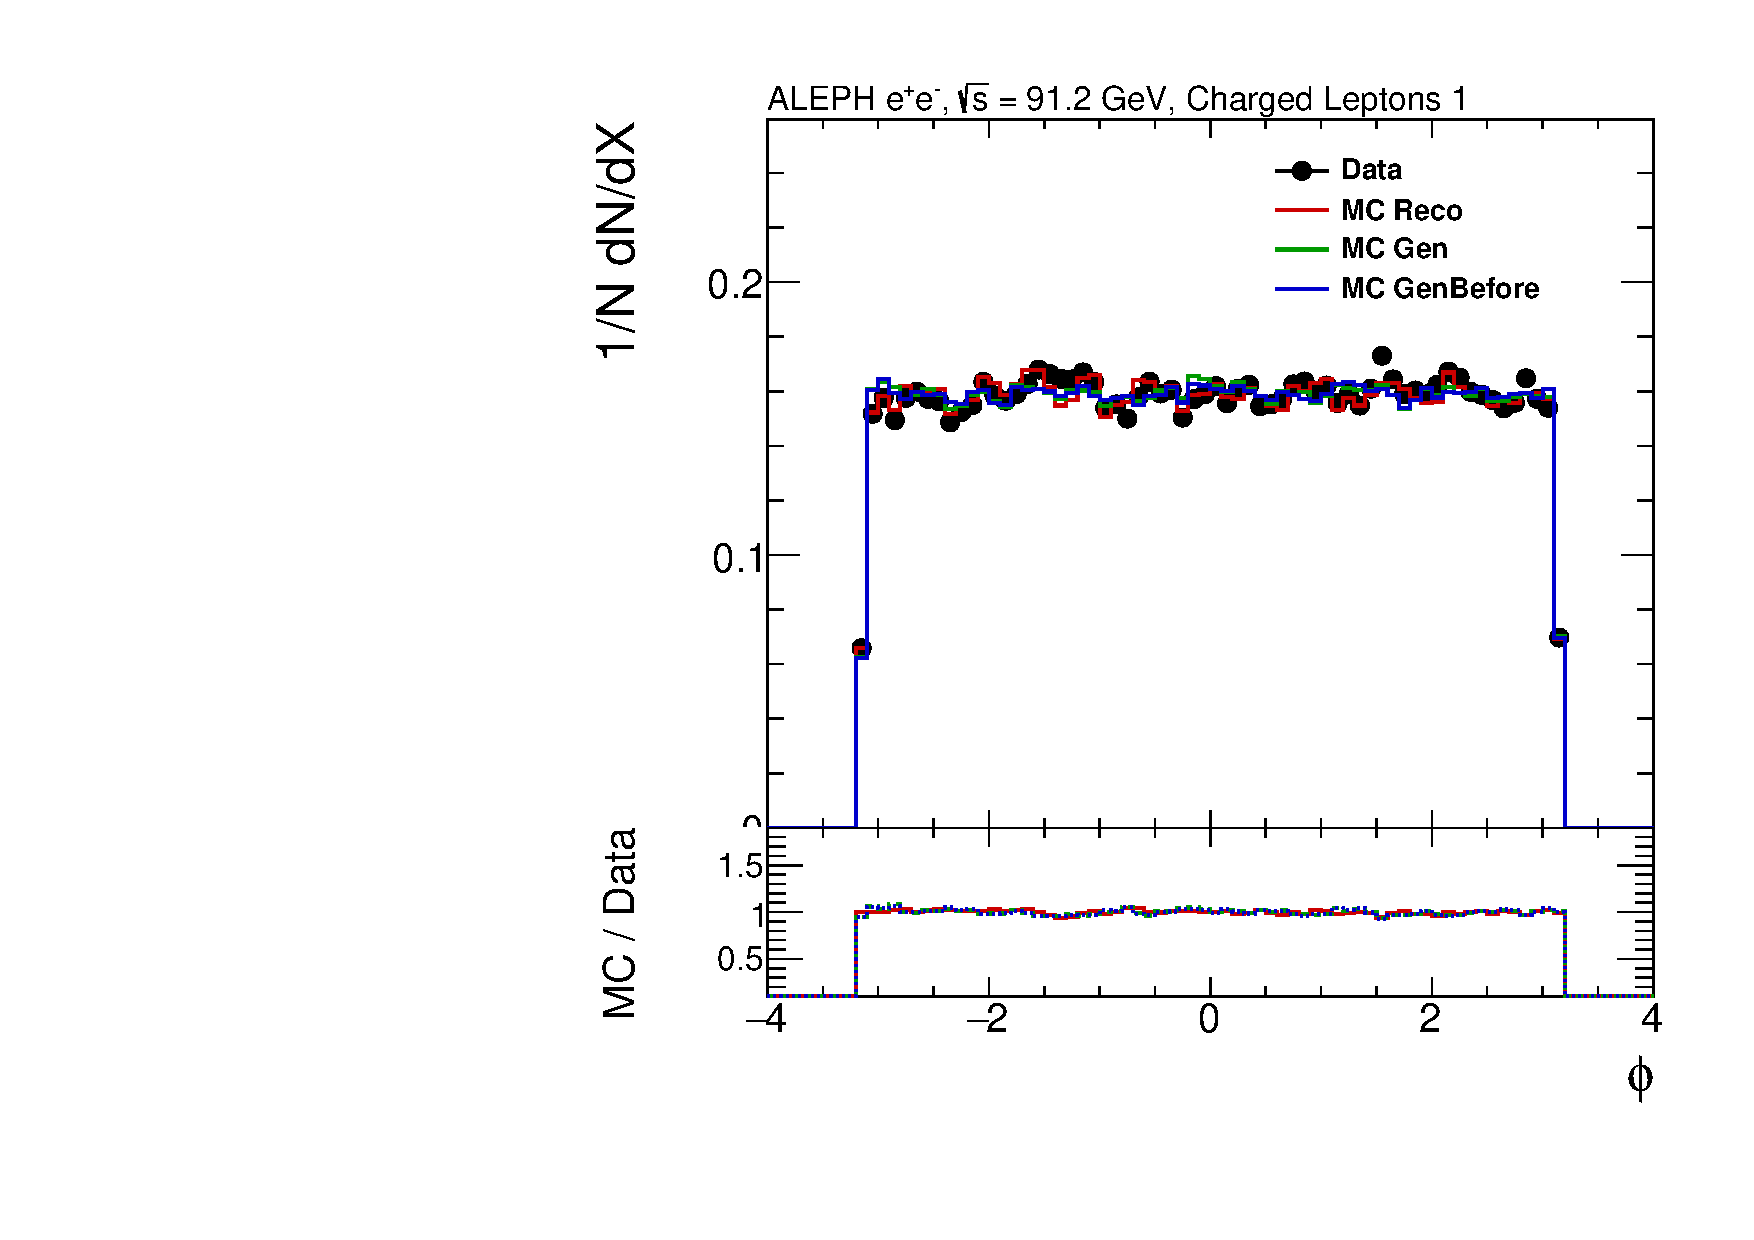
\includegraphics[width=0.242\textwidth]{figures/pwflag1_phi.pdf}
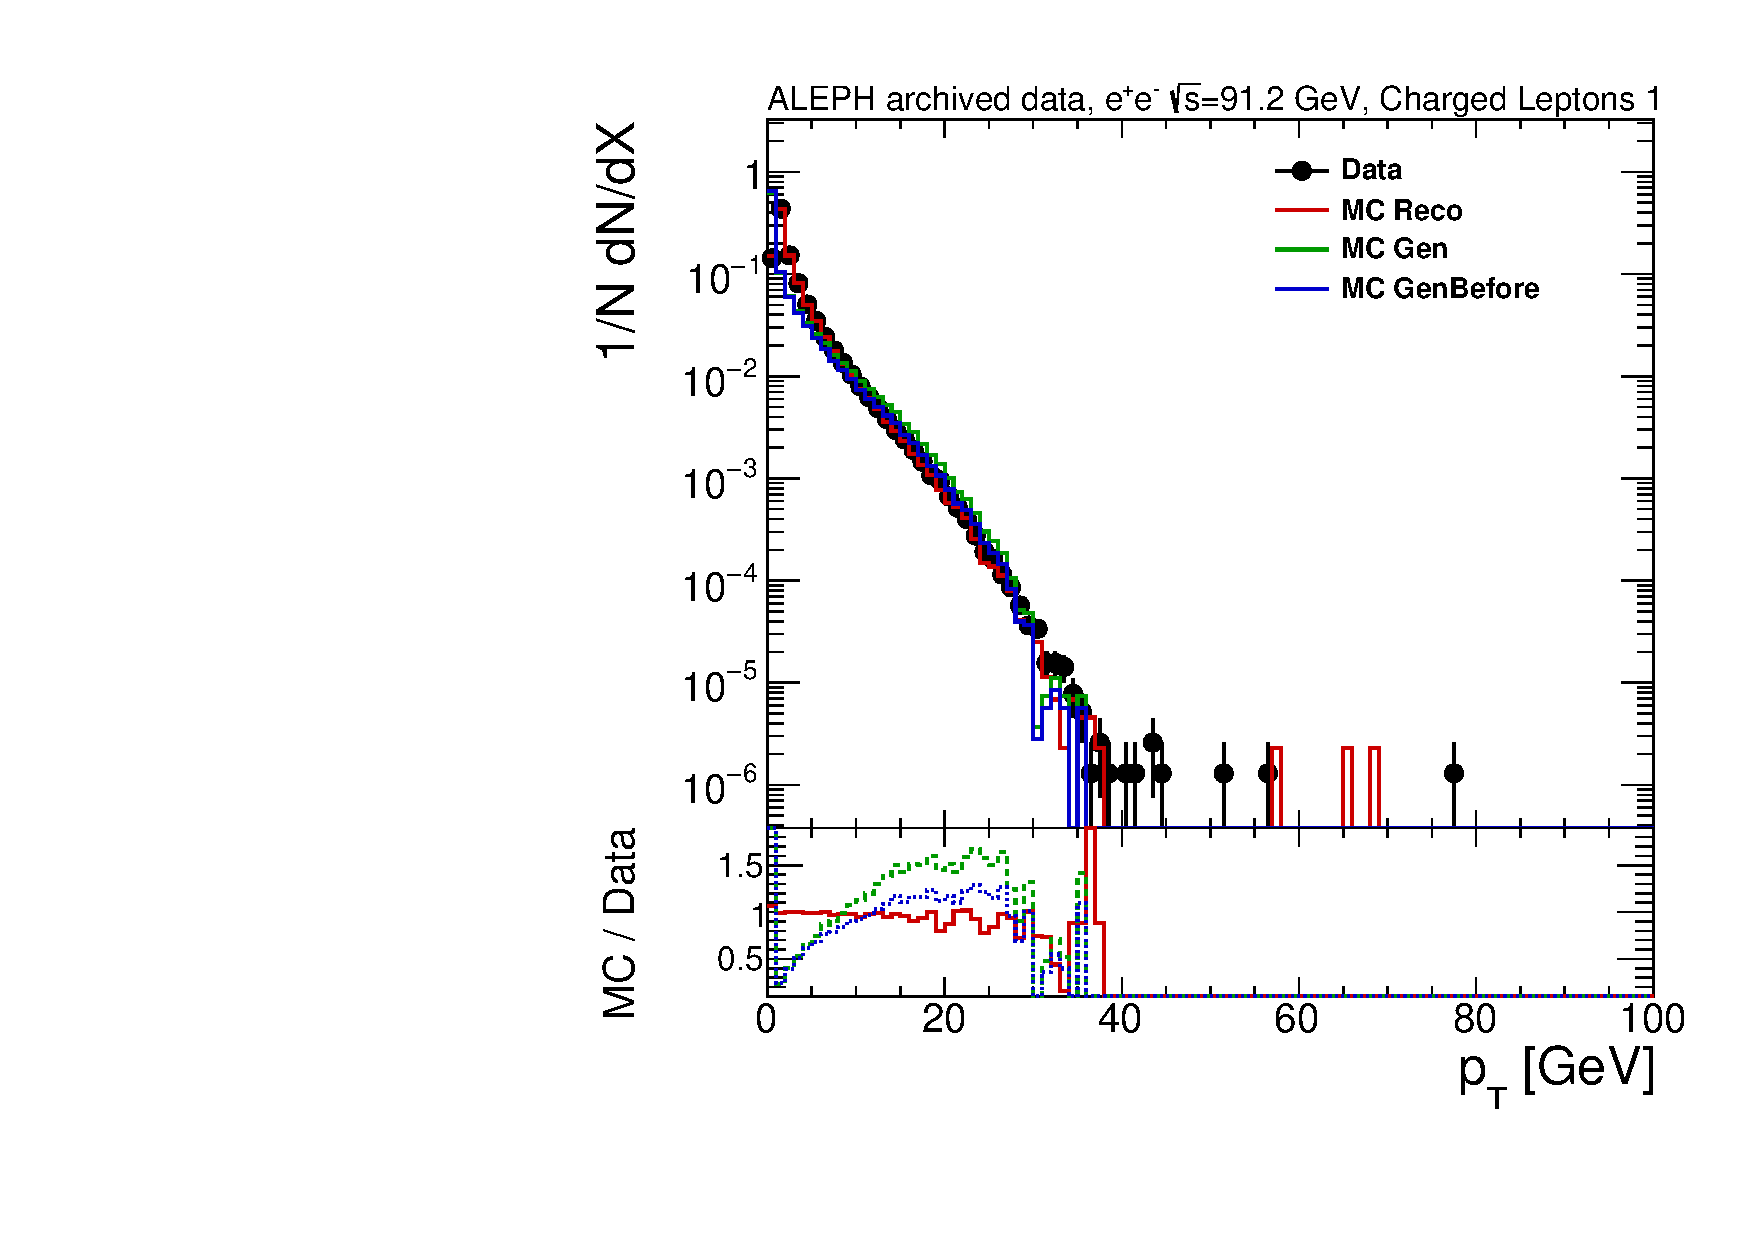
\includegraphics[width=0.242\textwidth]{figures/pwflag1_pt.pdf}
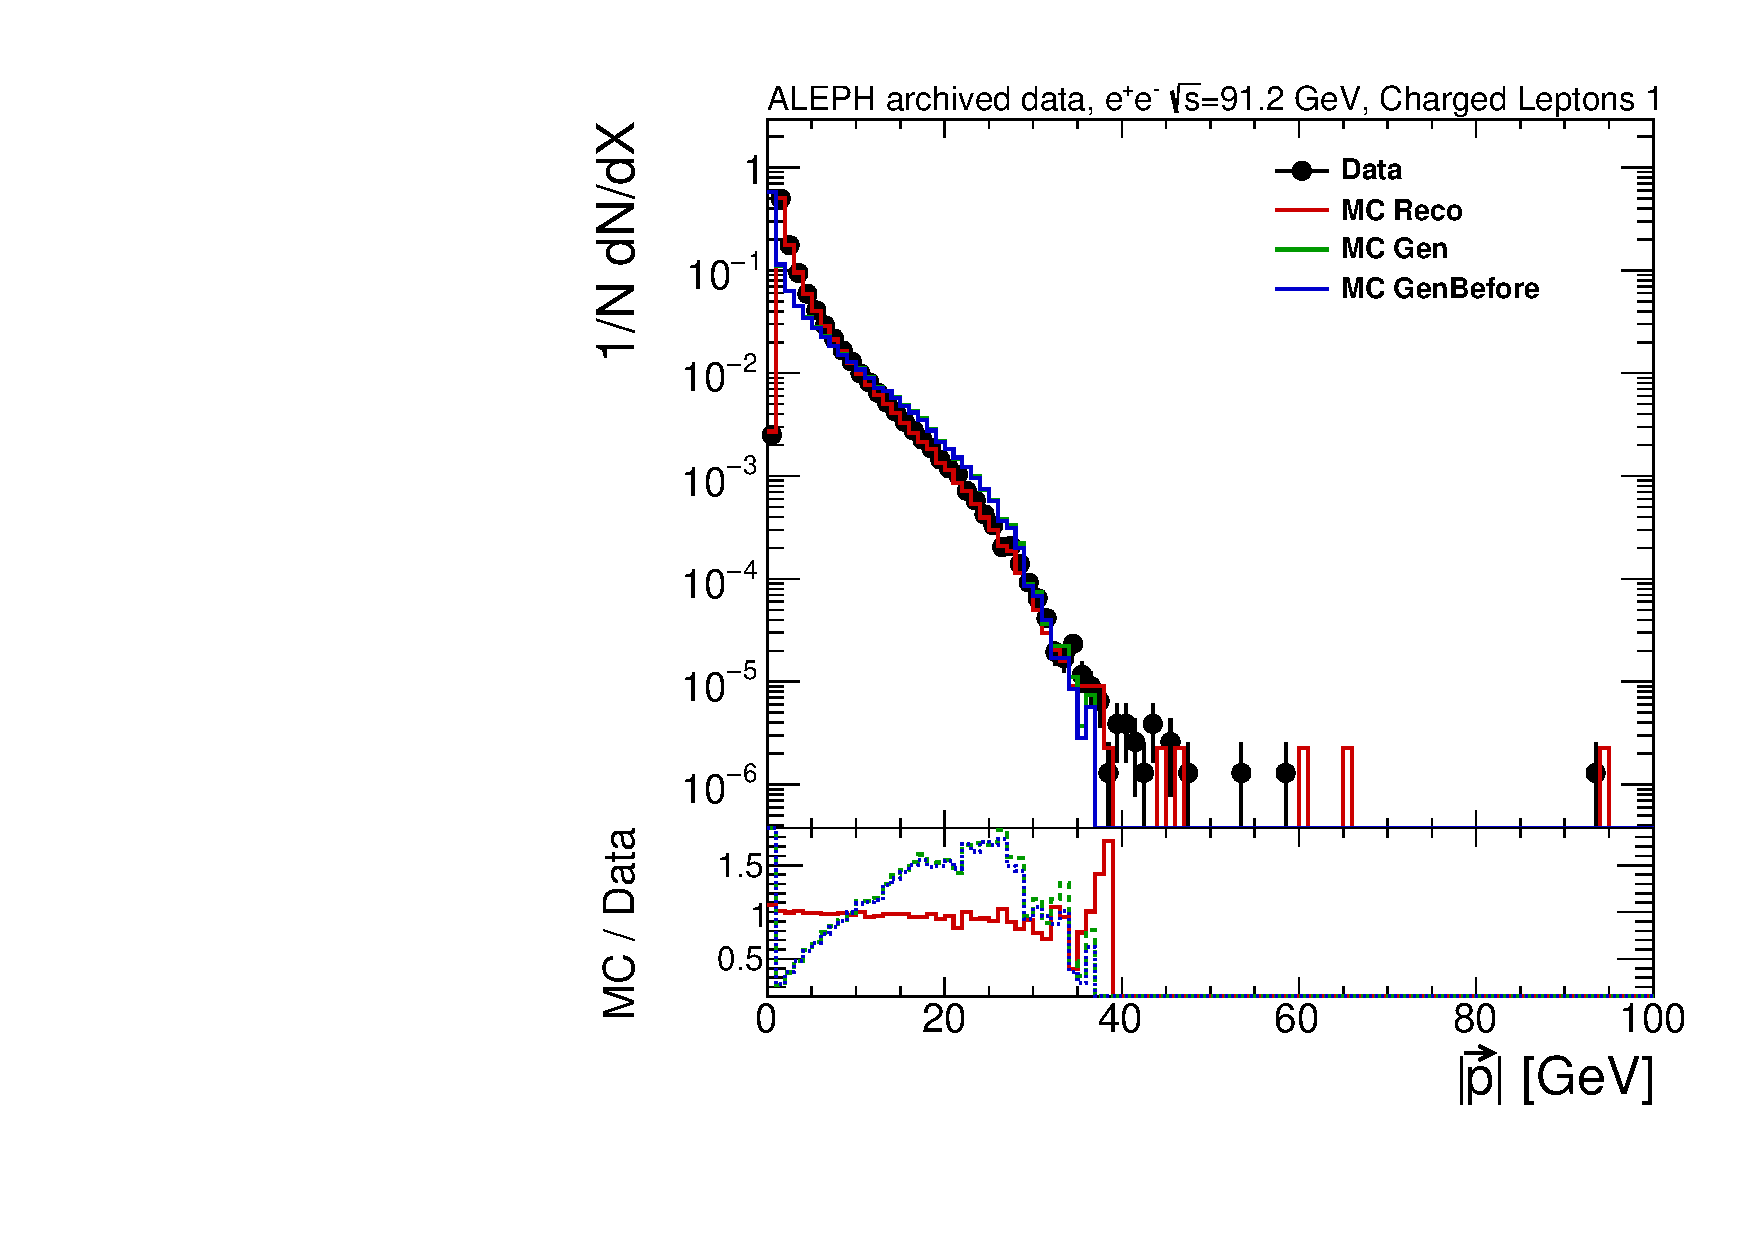
\includegraphics[width=0.242\textwidth]{figures/pwflag1_pmag.pdf}
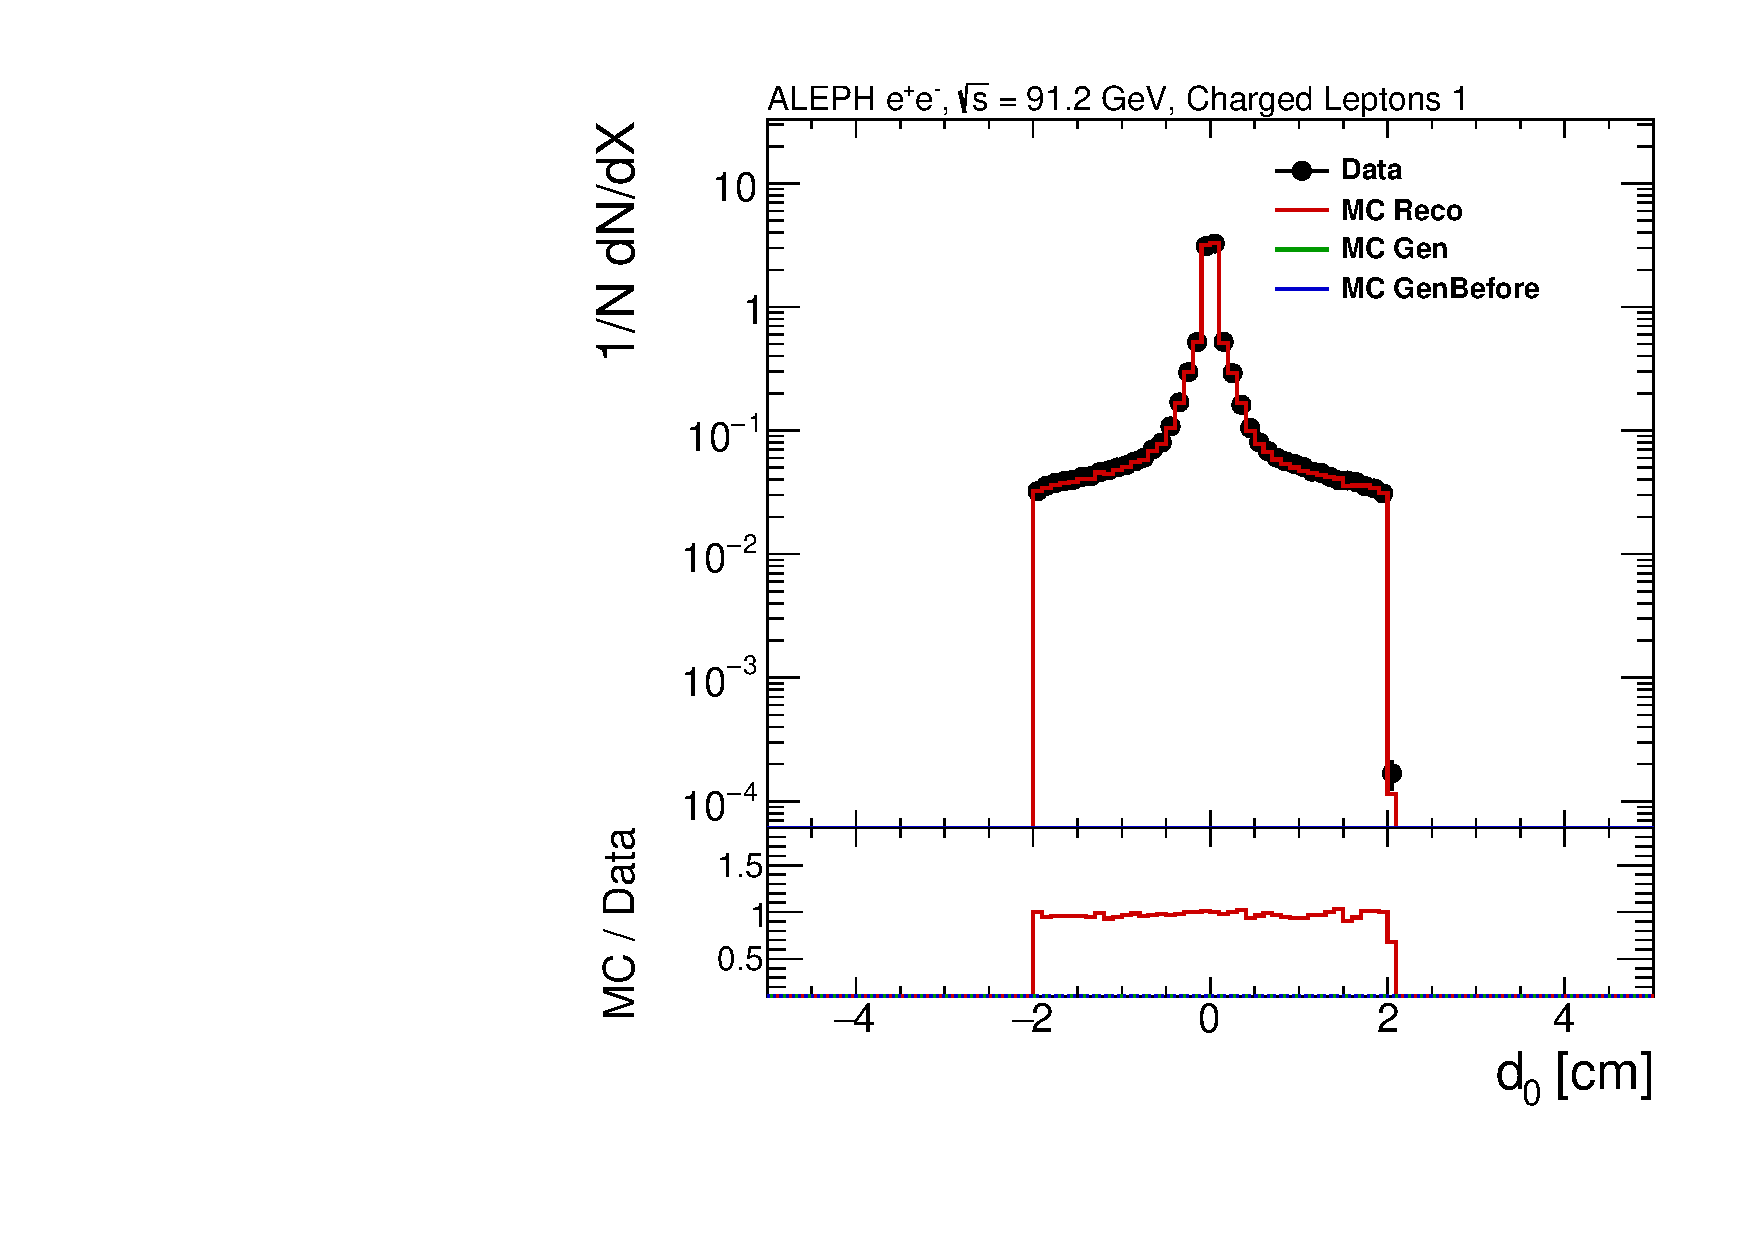
\includegraphics[width=0.242\textwidth]{figures/pwflag1_d0.pdf}
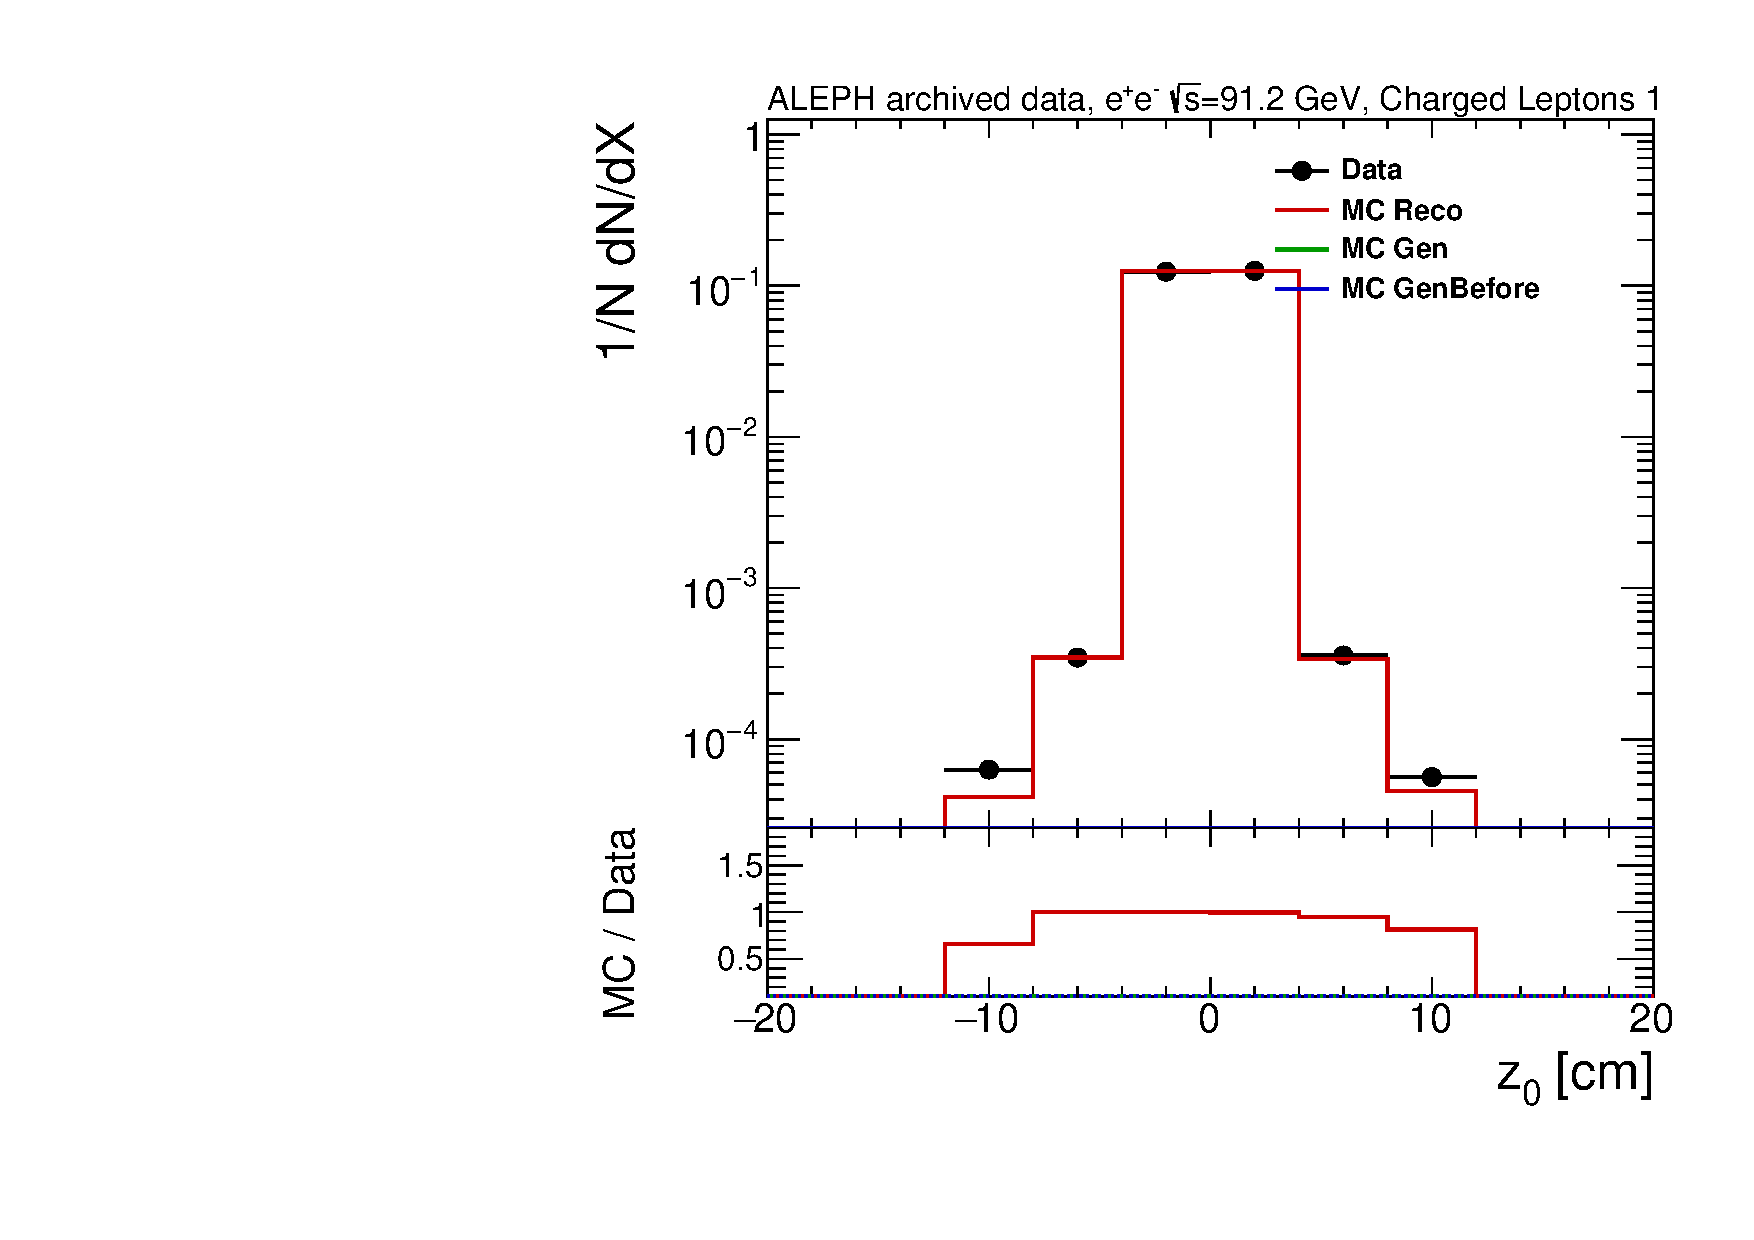
\includegraphics[width=0.242\textwidth]{figures/pwflag1_z0.pdf}
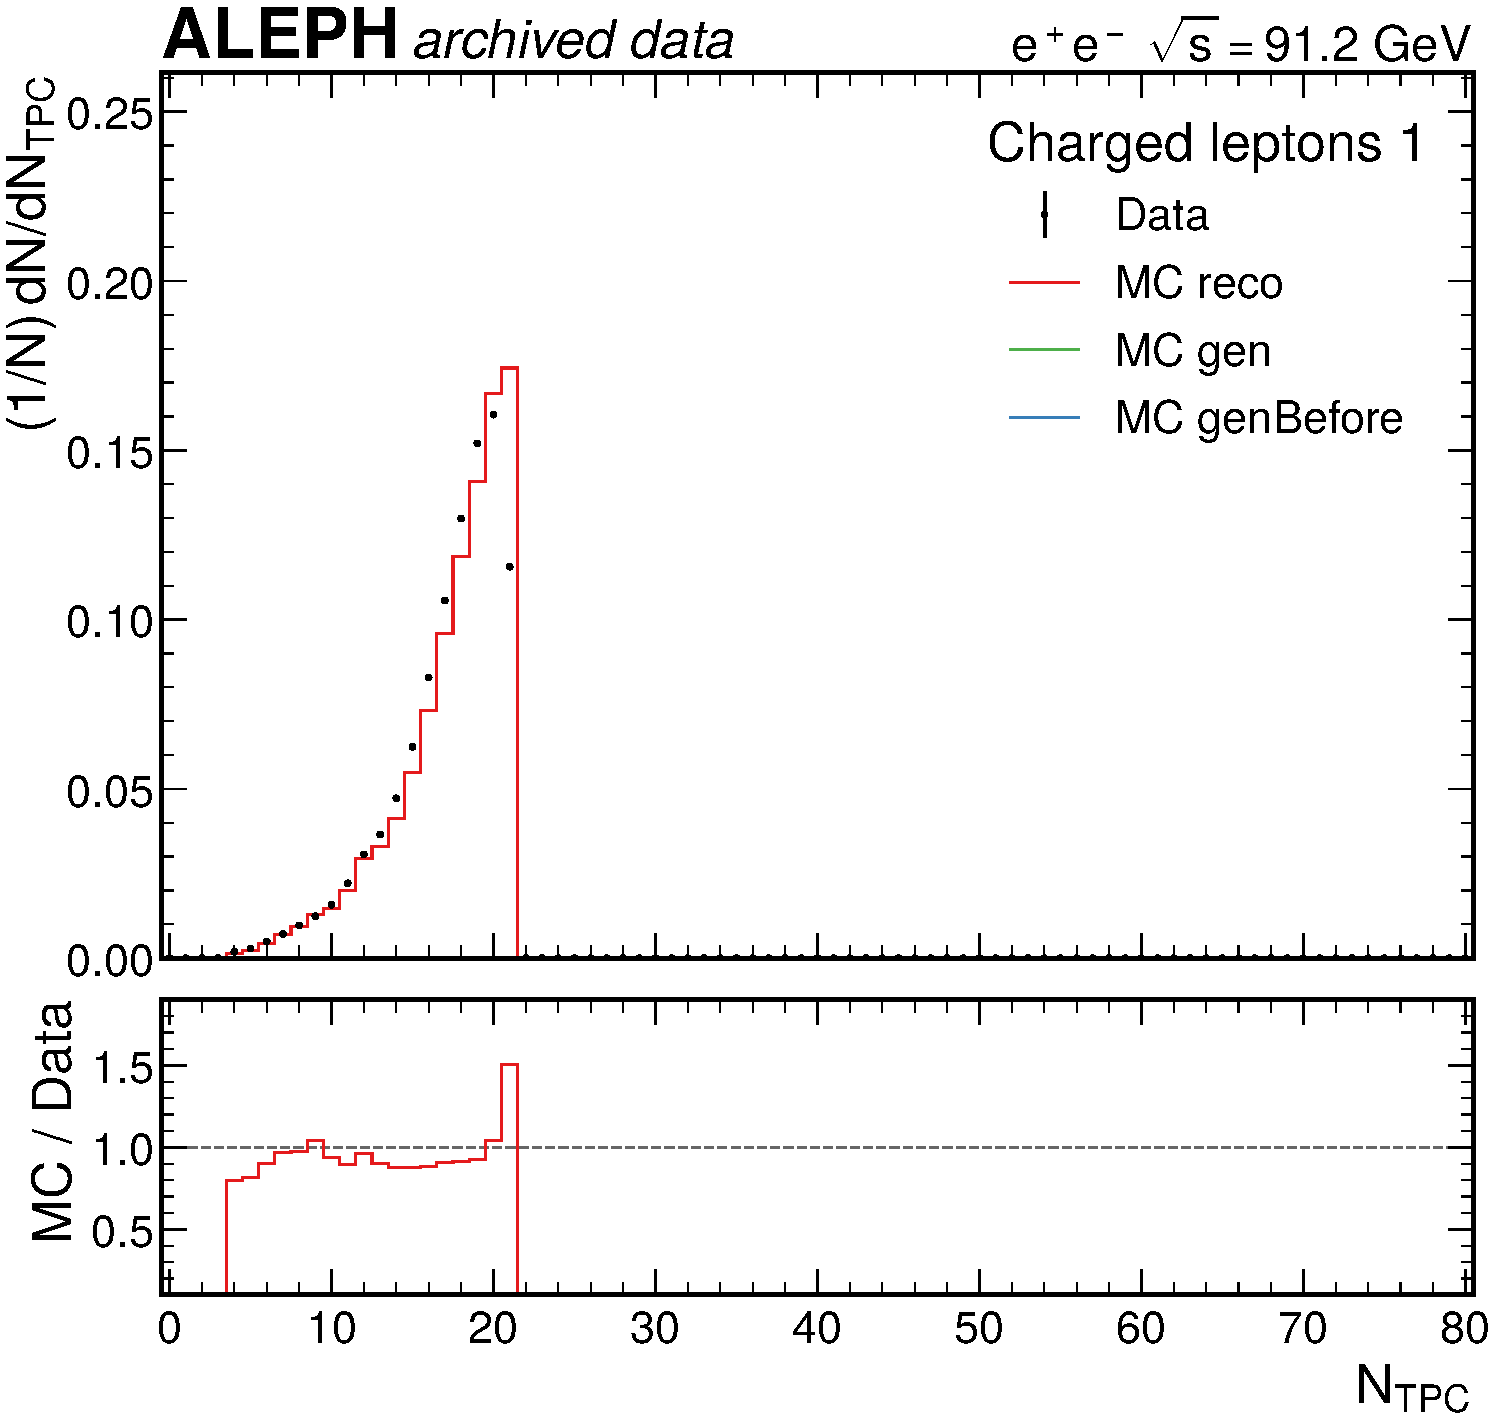
\includegraphics[width=0.242\textwidth]{figures/pwflag1_ntpc.pdf}
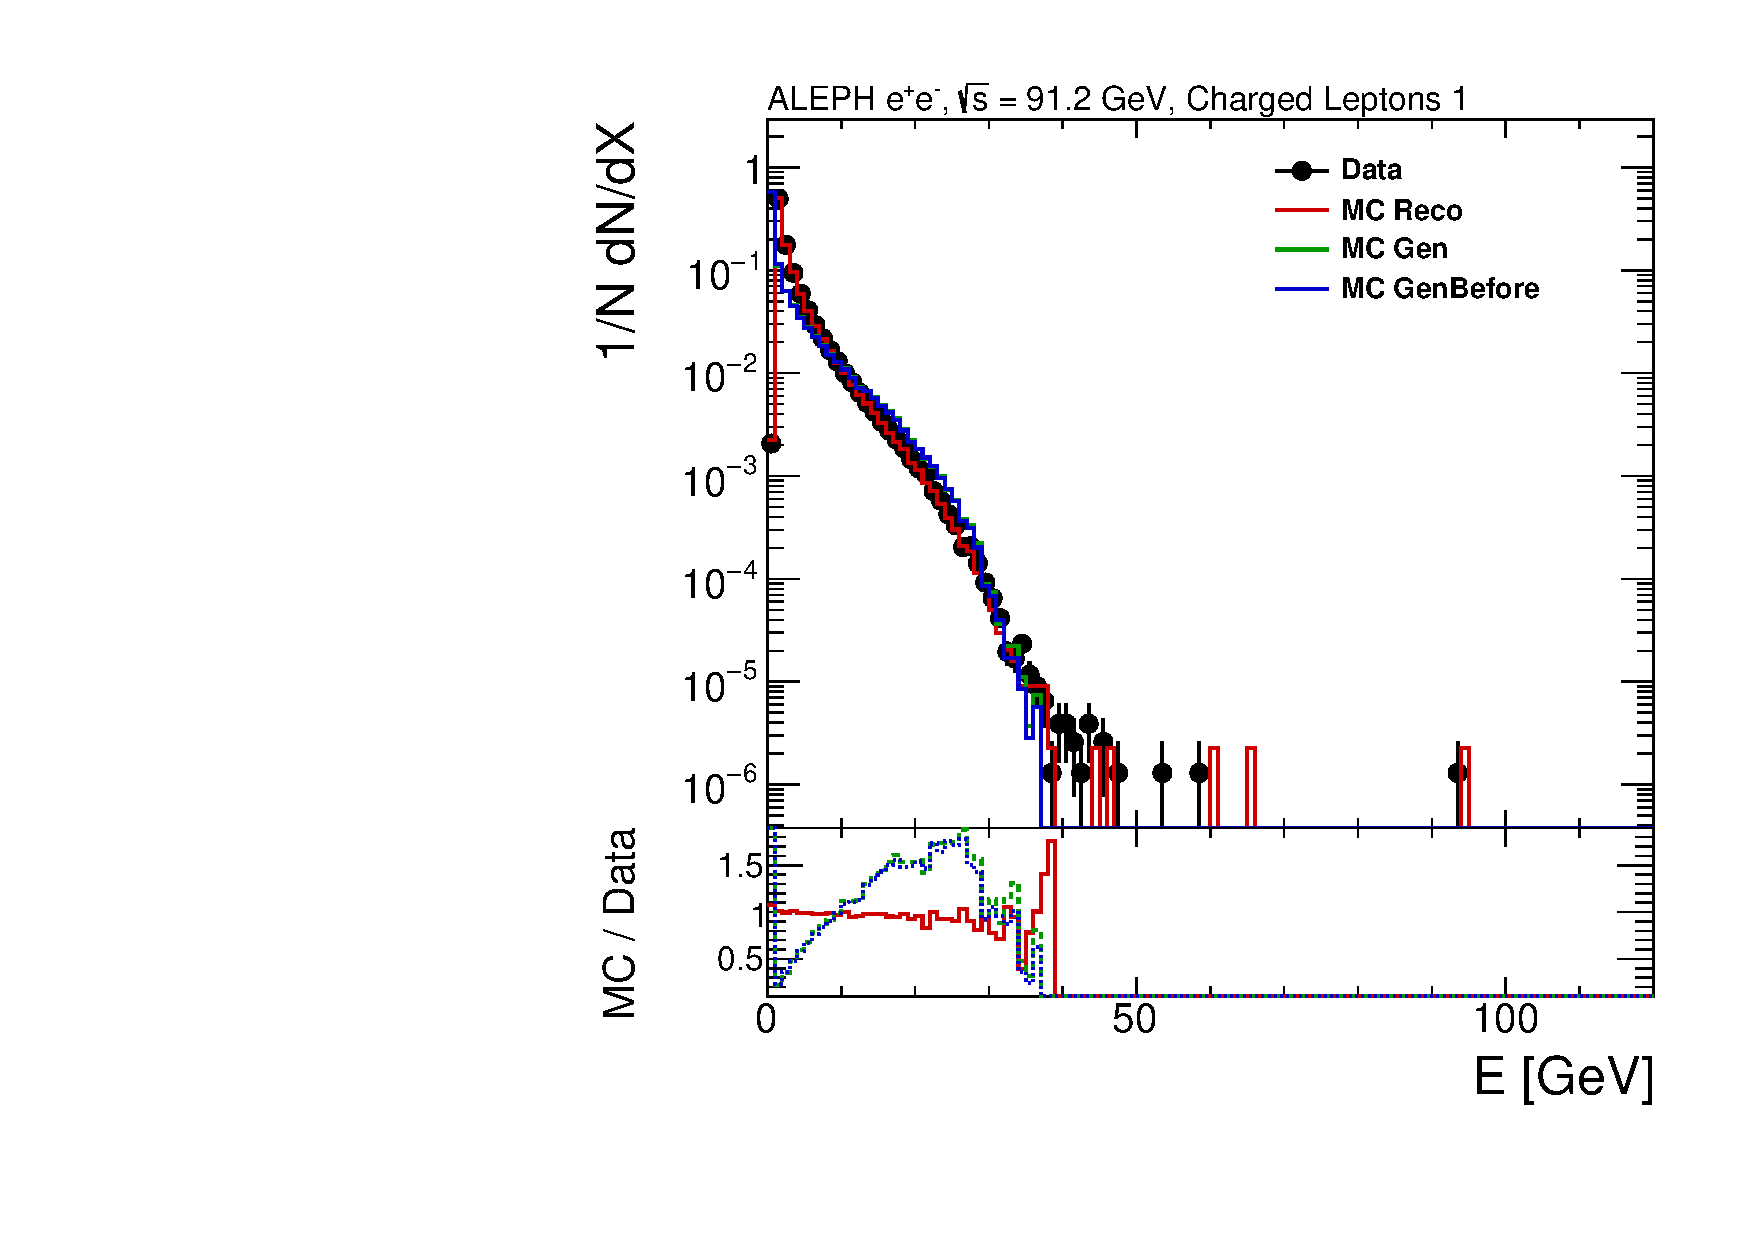
\includegraphics[width=0.242\textwidth]{figures/pwflag1_energy.pdf}
% 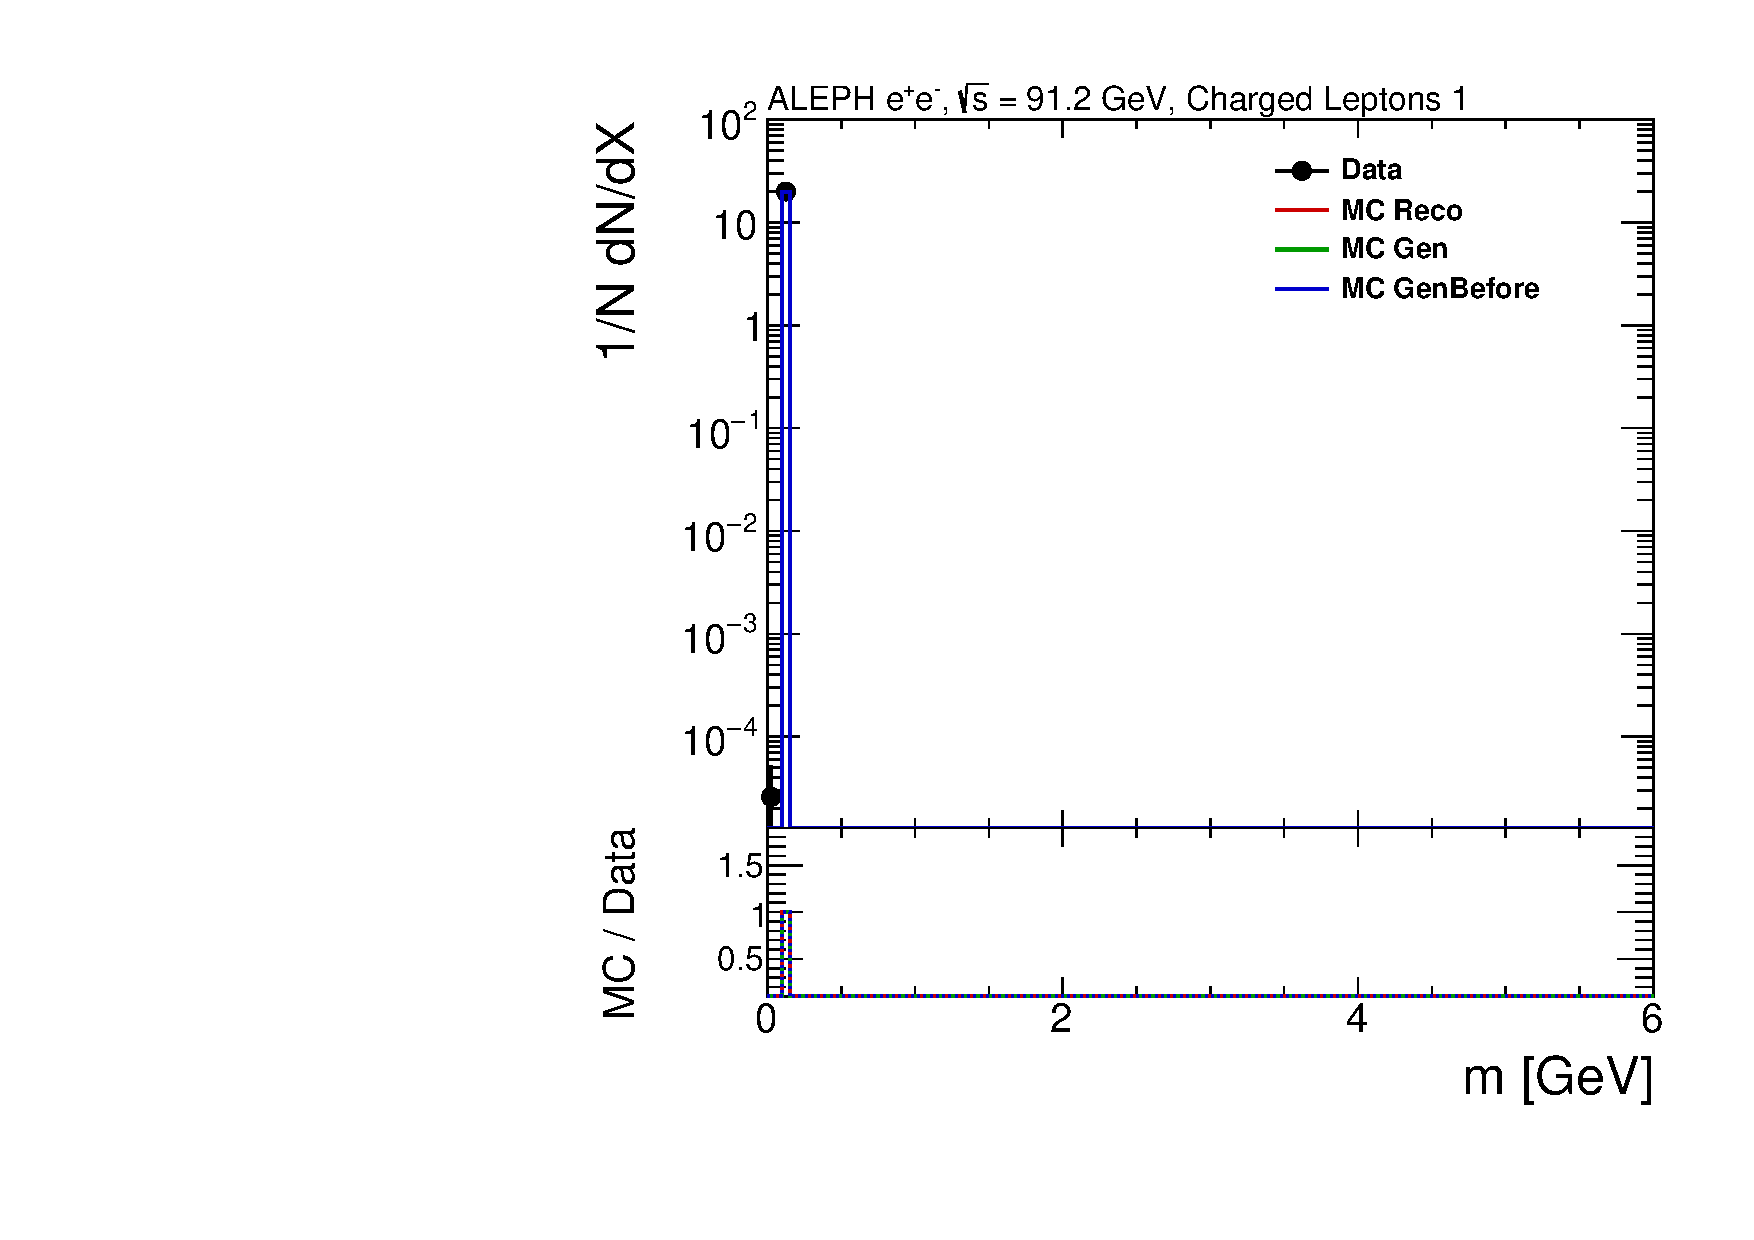
\includegraphics[width=0.242\textwidth]{figures/pwflag1_mass.pdf}
\caption{Complete \texttt{pwflag}=1 kinematic set.}
\label{fig:pwflag1_full}
\end{figure}

\begin{figure}[t!]
\centering
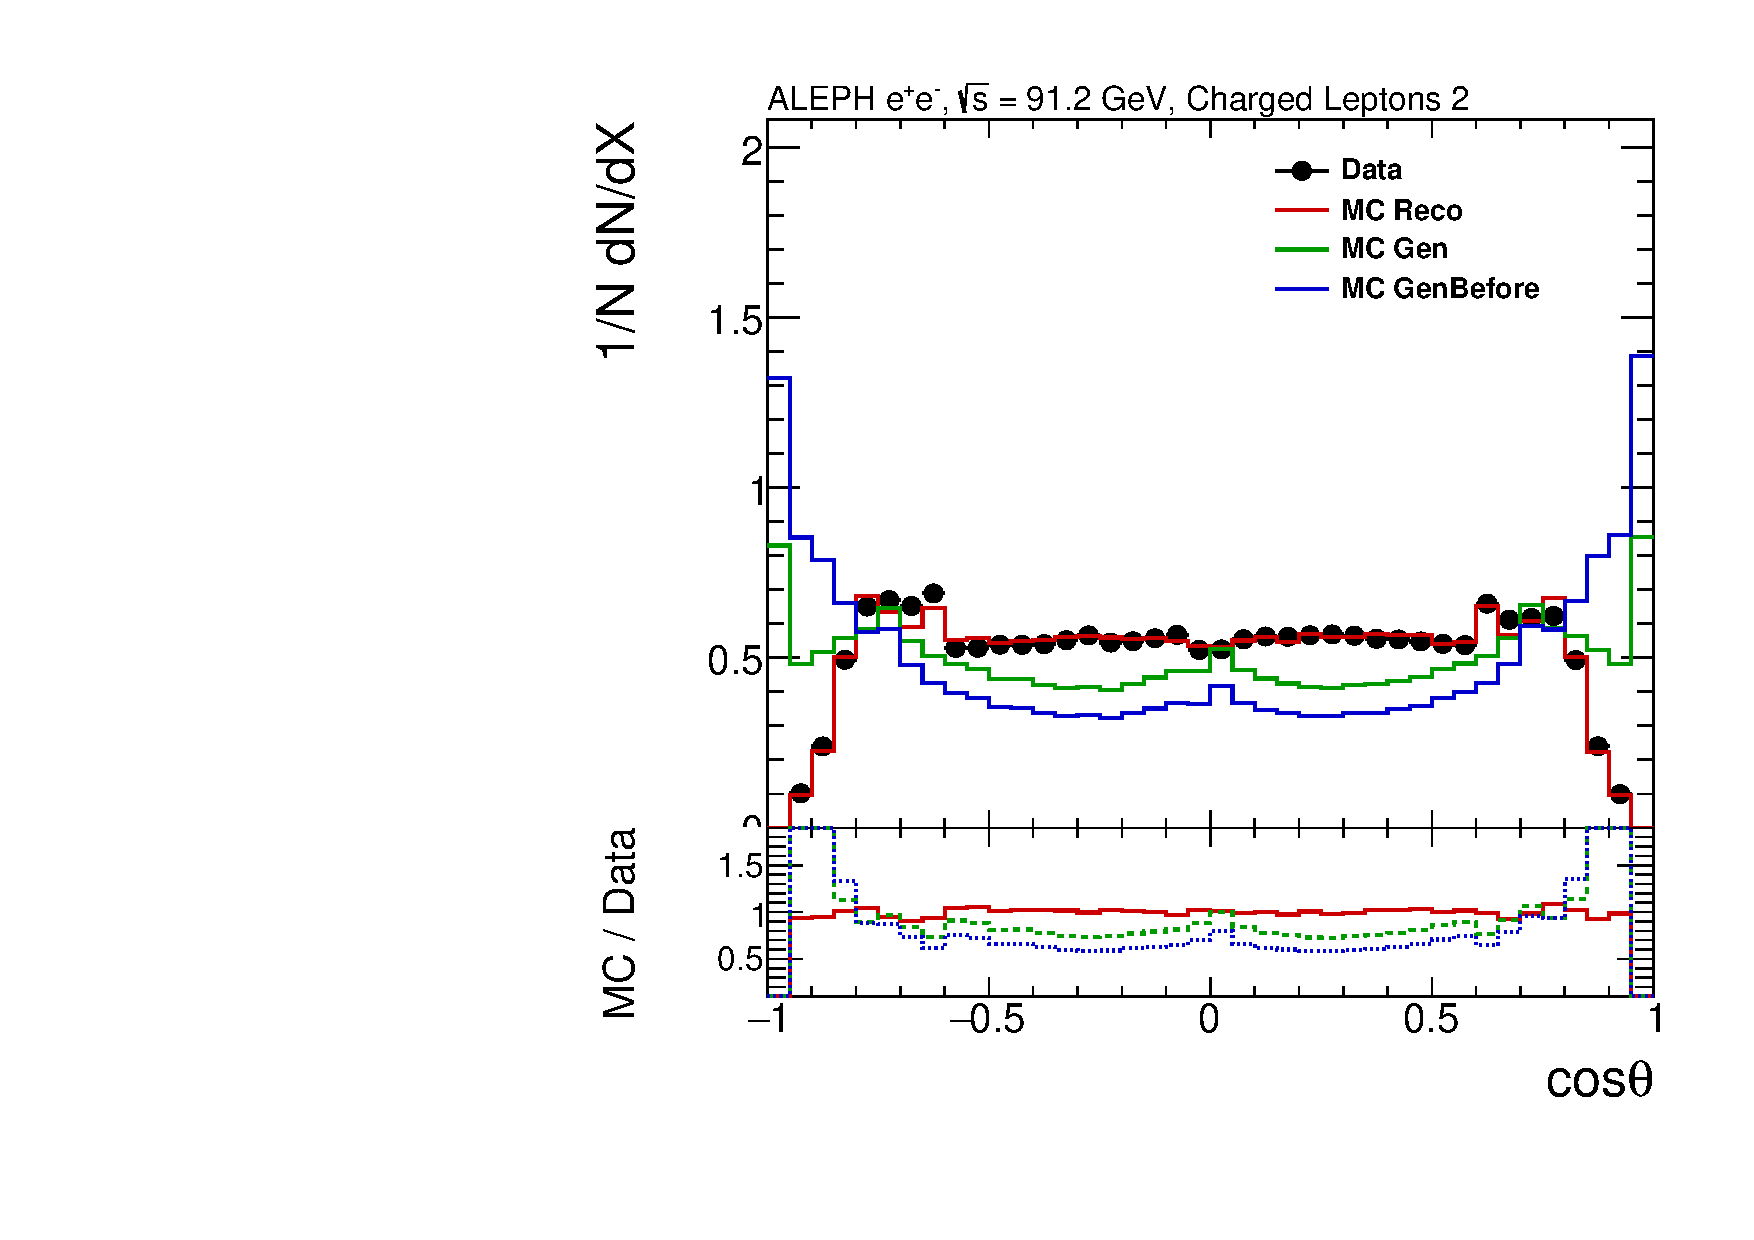
\includegraphics[width=0.242\textwidth]{figures/pwflag2_cosTheta.pdf}
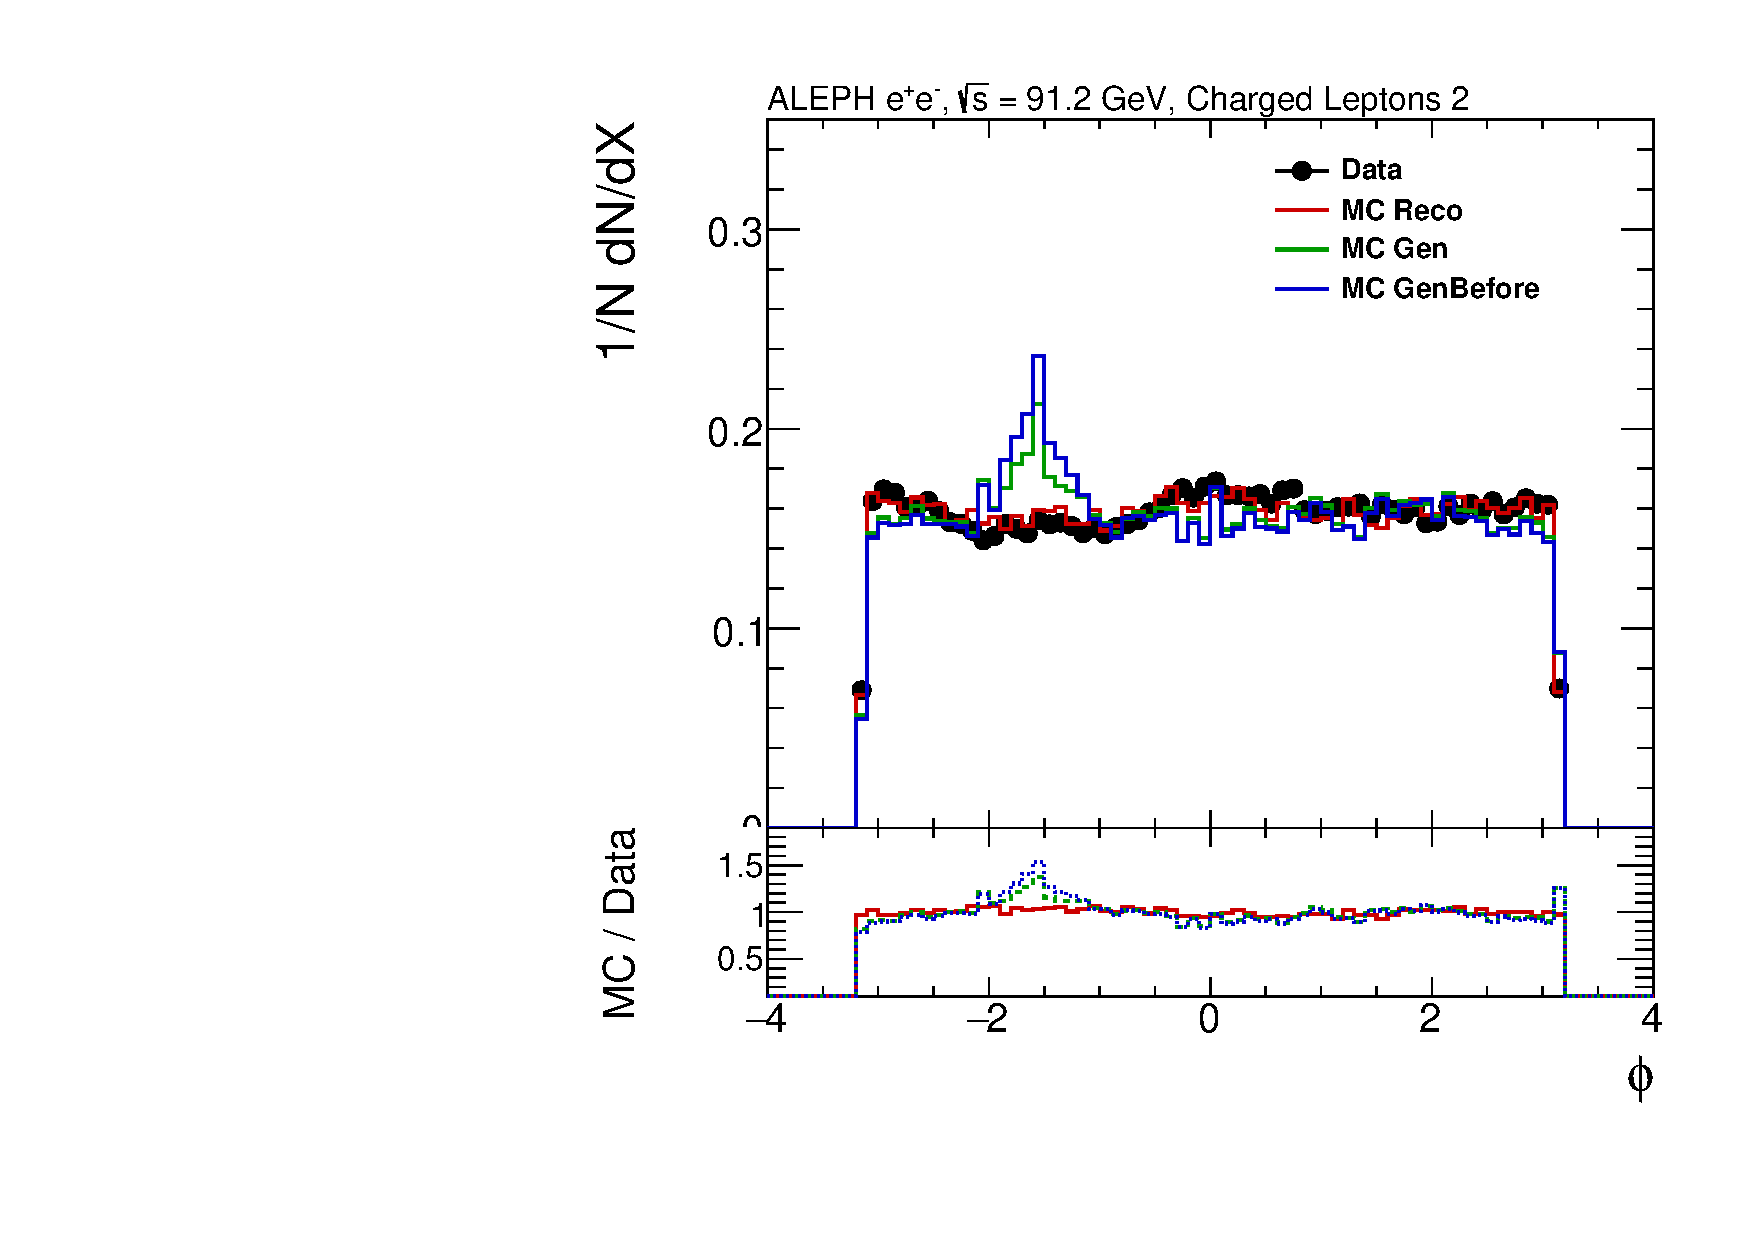
\includegraphics[width=0.242\textwidth]{figures/pwflag2_phi.pdf}
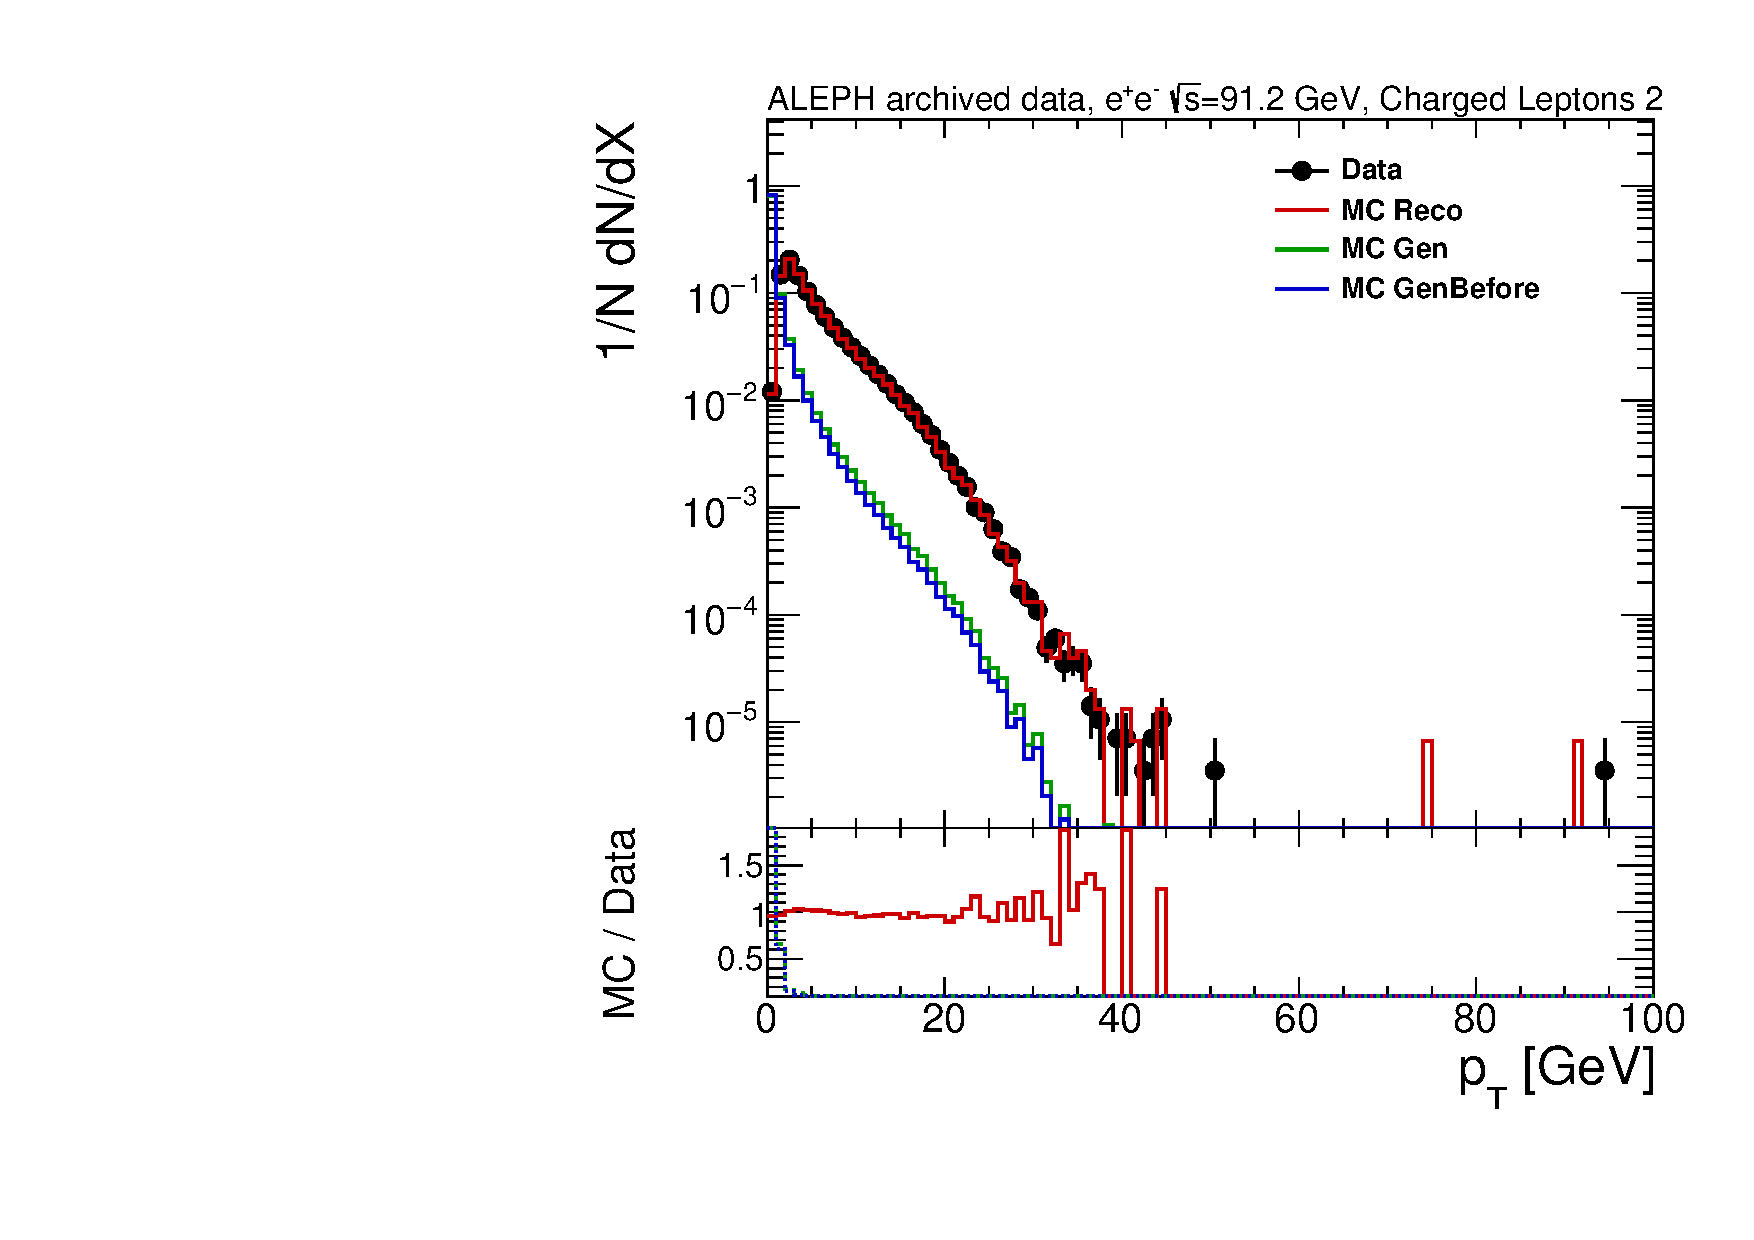
\includegraphics[width=0.242\textwidth]{figures/pwflag2_pt.pdf}
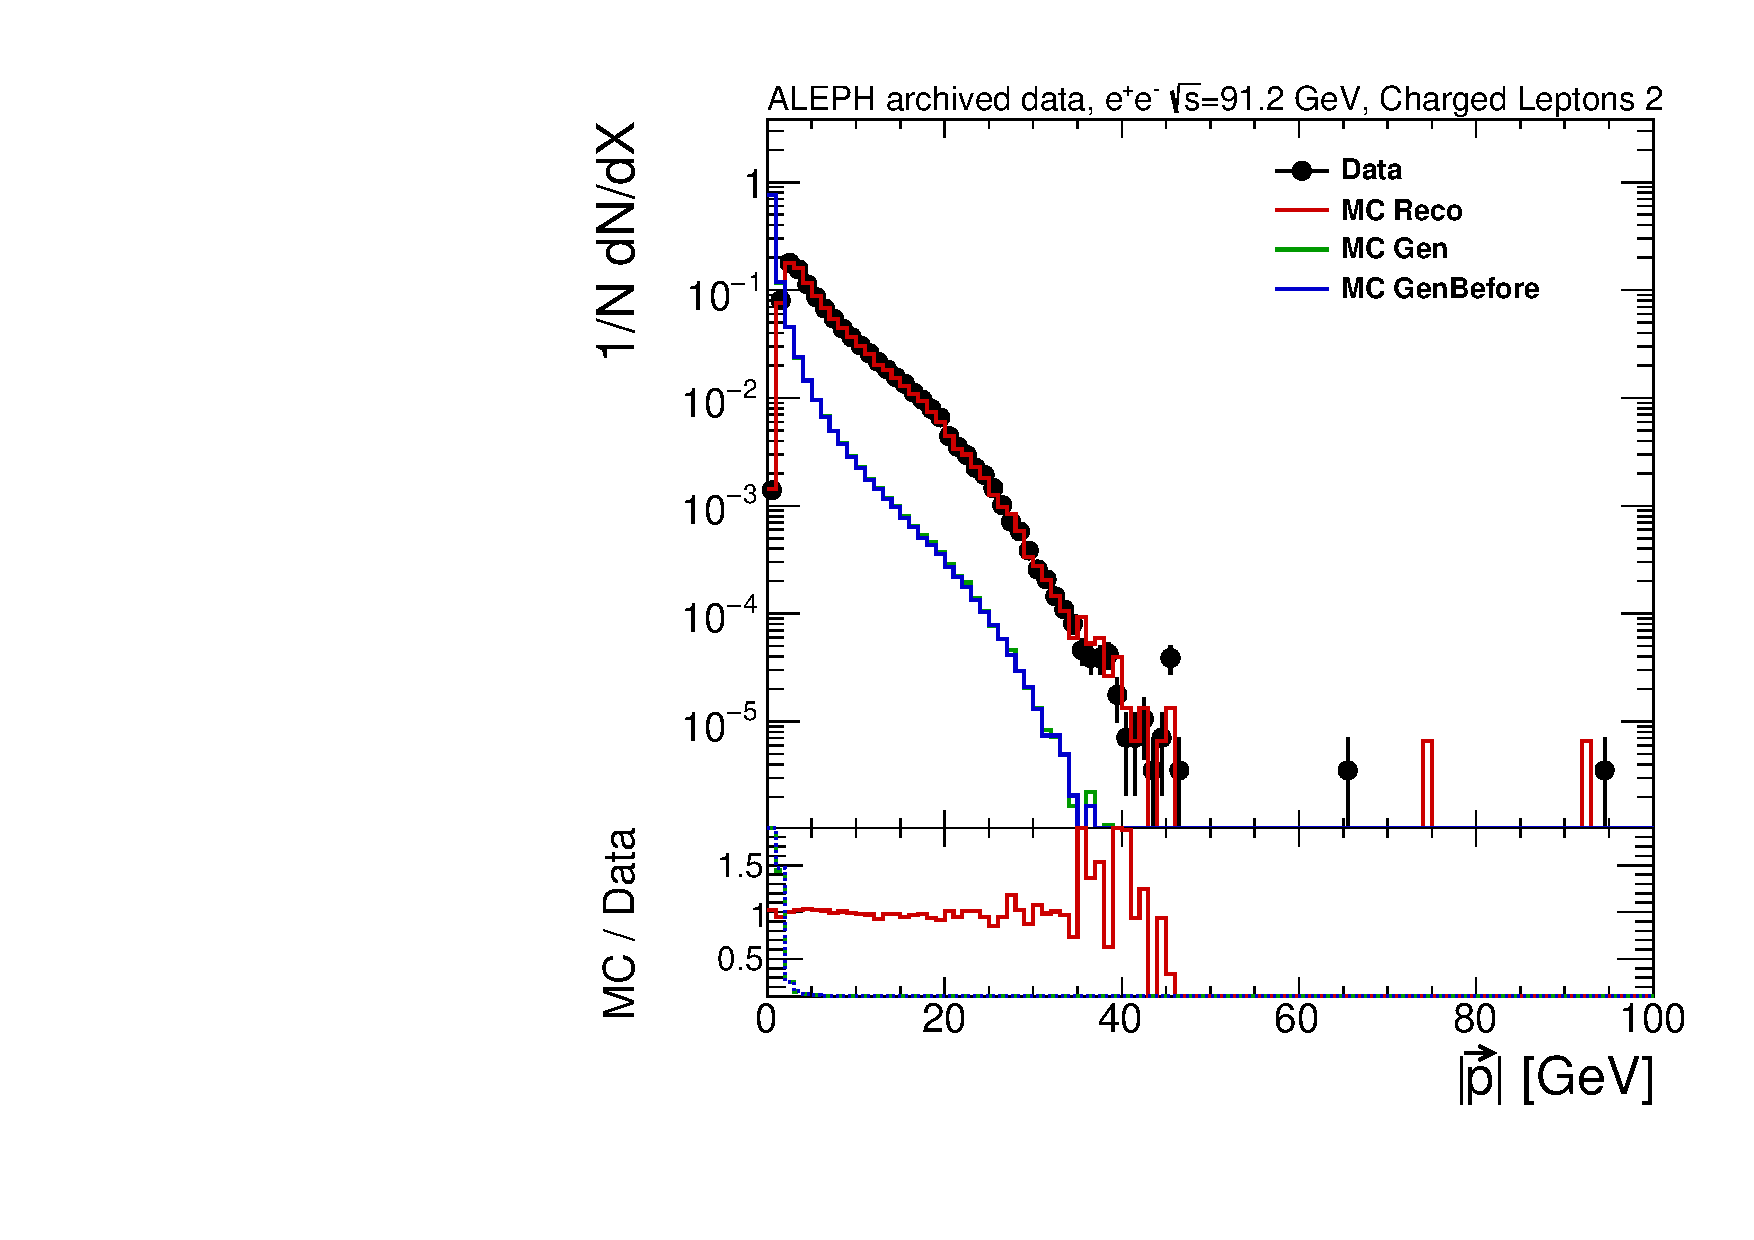
\includegraphics[width=0.242\textwidth]{figures/pwflag2_pmag.pdf}
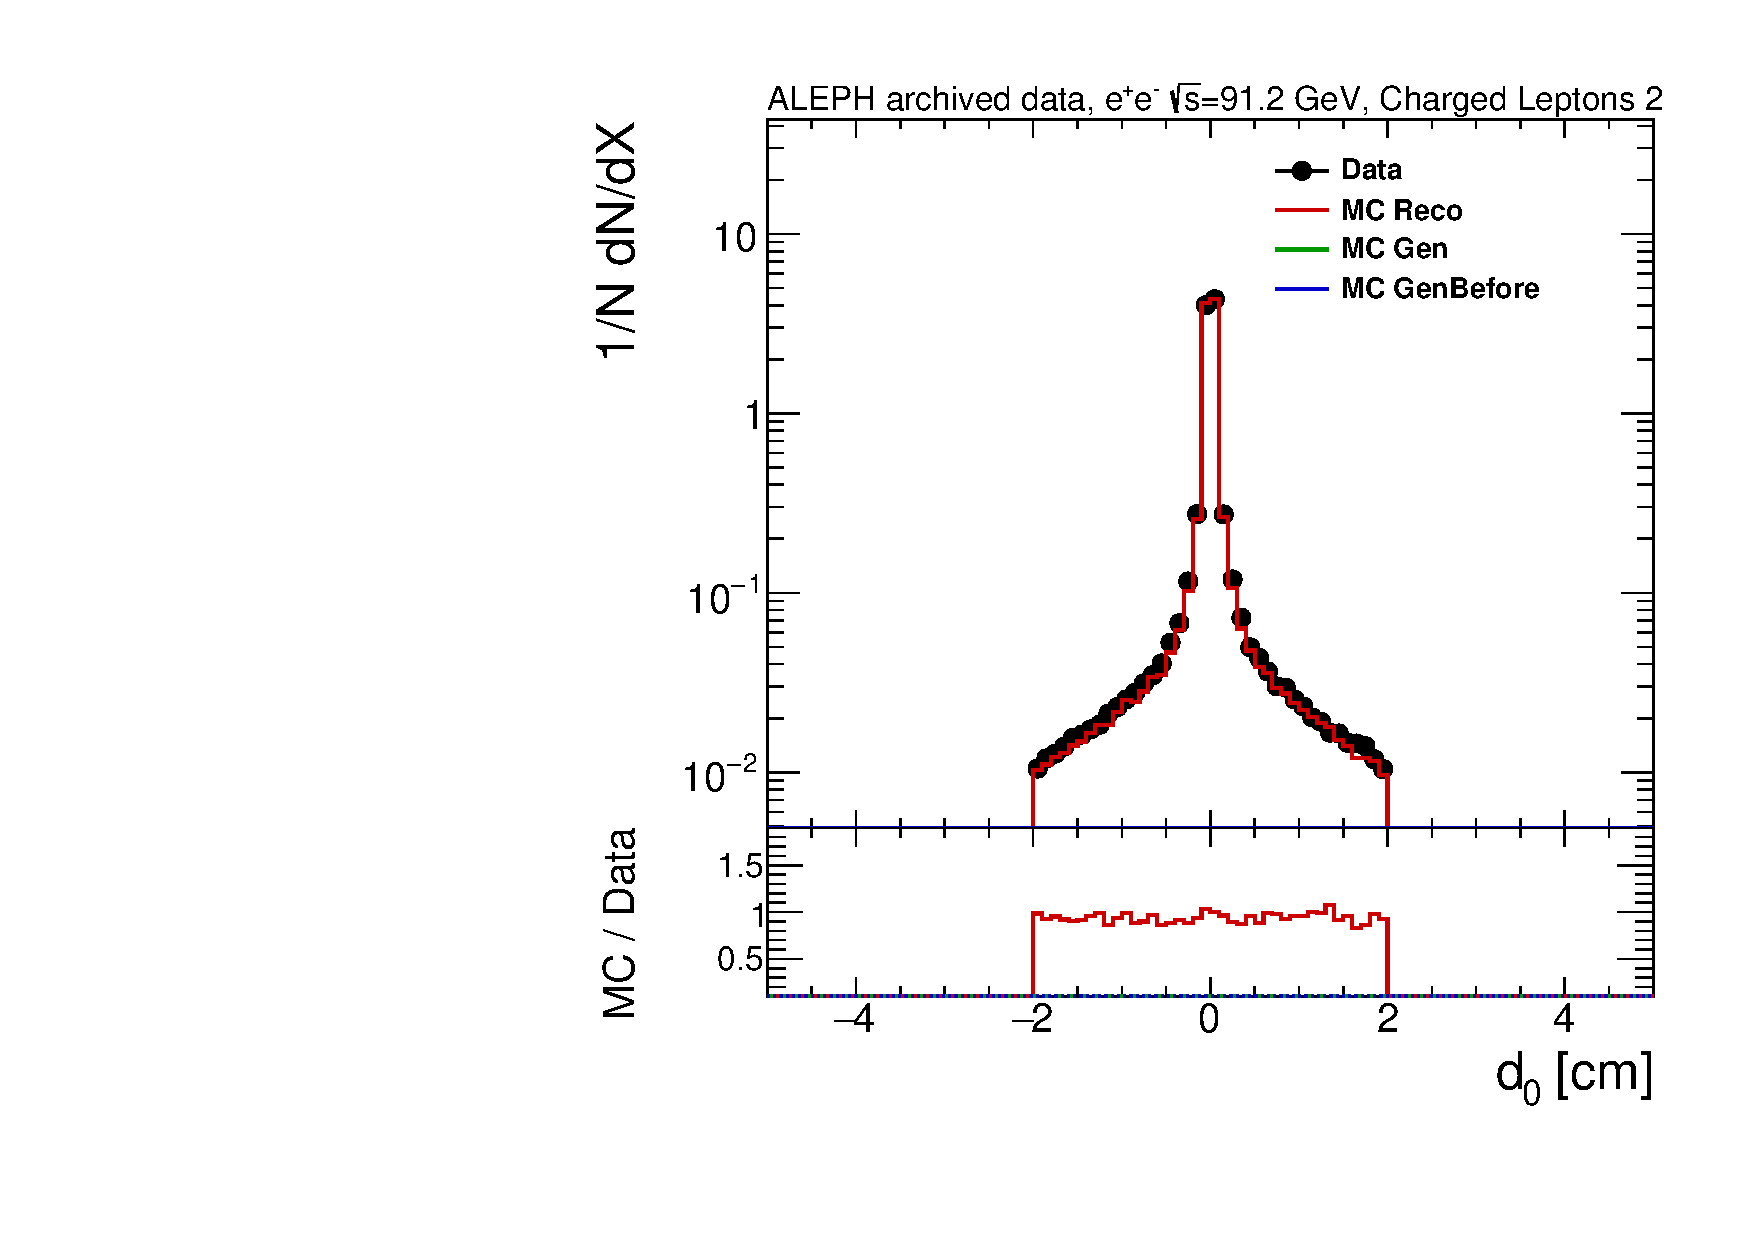
\includegraphics[width=0.242\textwidth]{figures/pwflag2_d0.pdf}
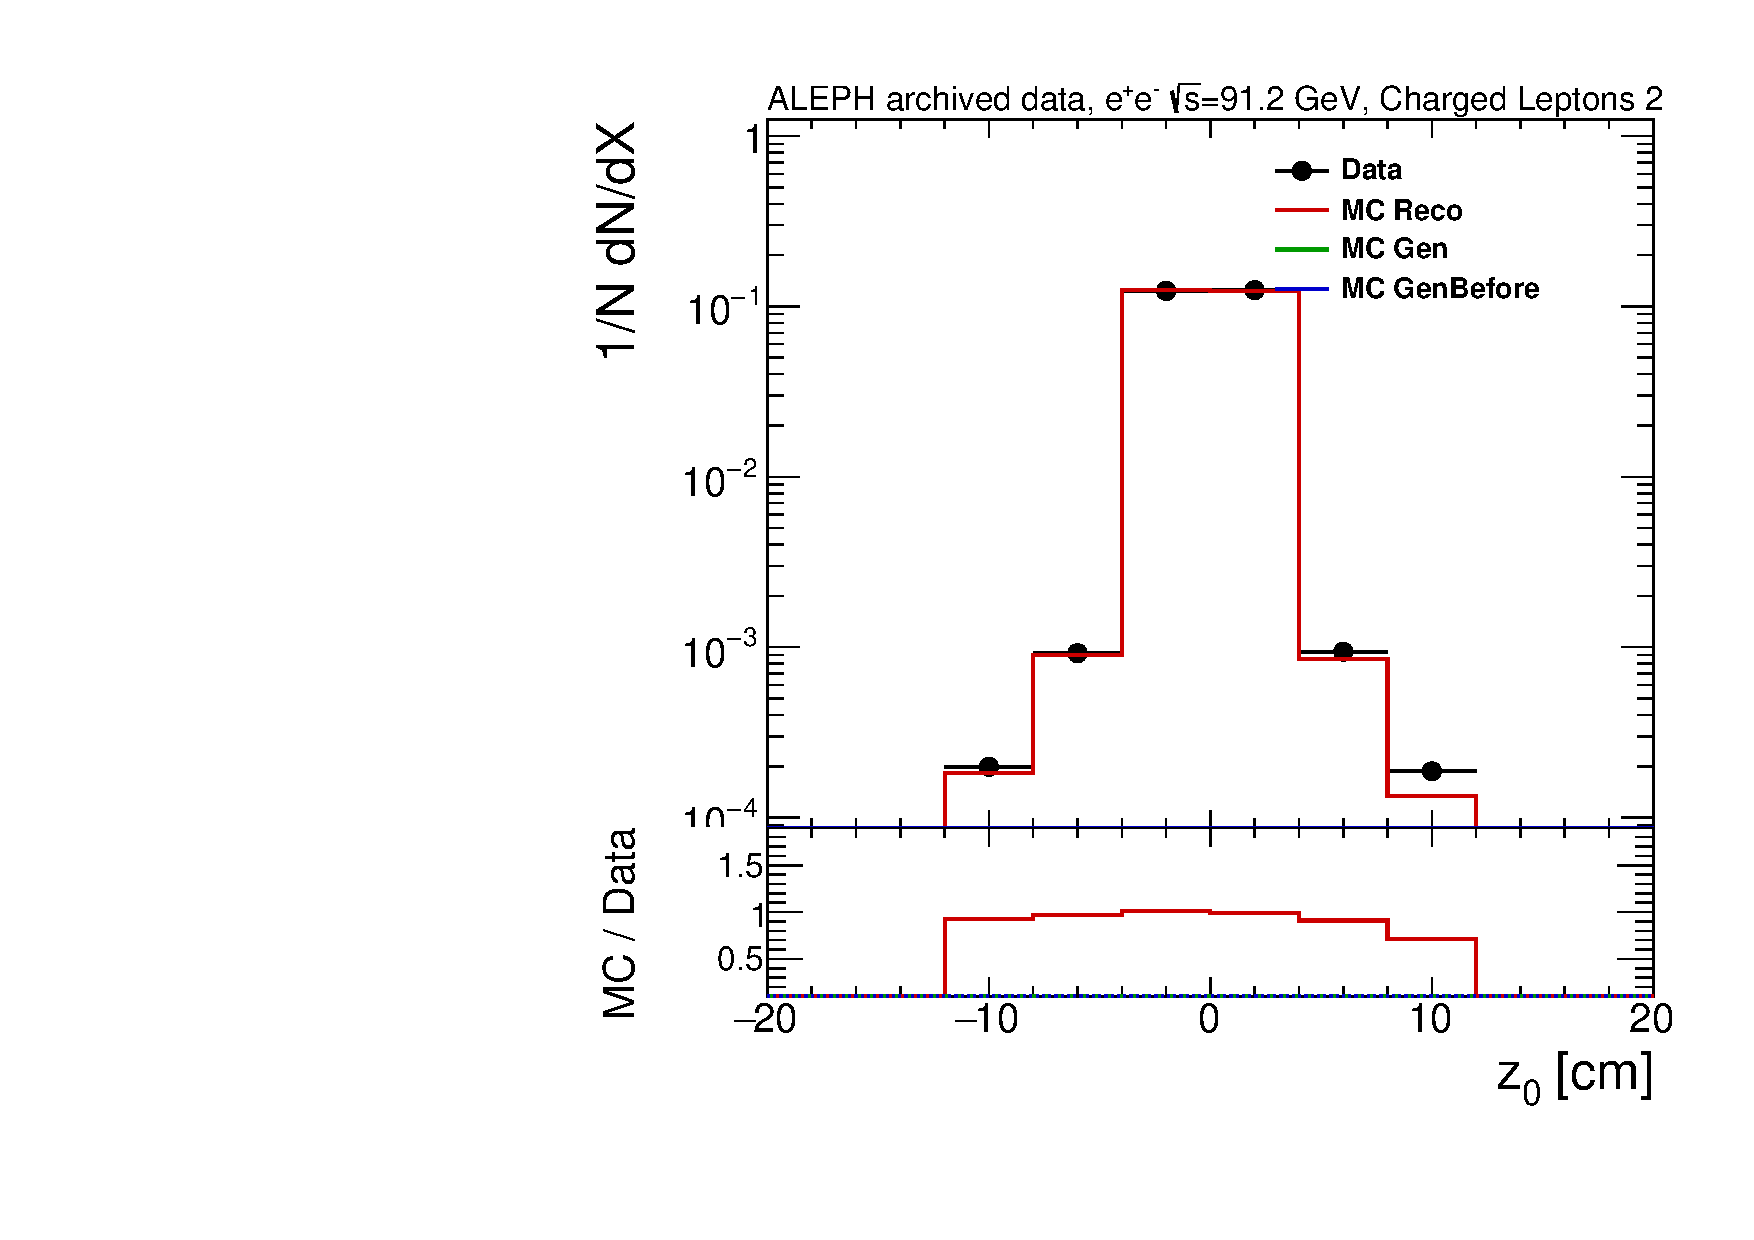
\includegraphics[width=0.242\textwidth]{figures/pwflag2_z0.pdf}
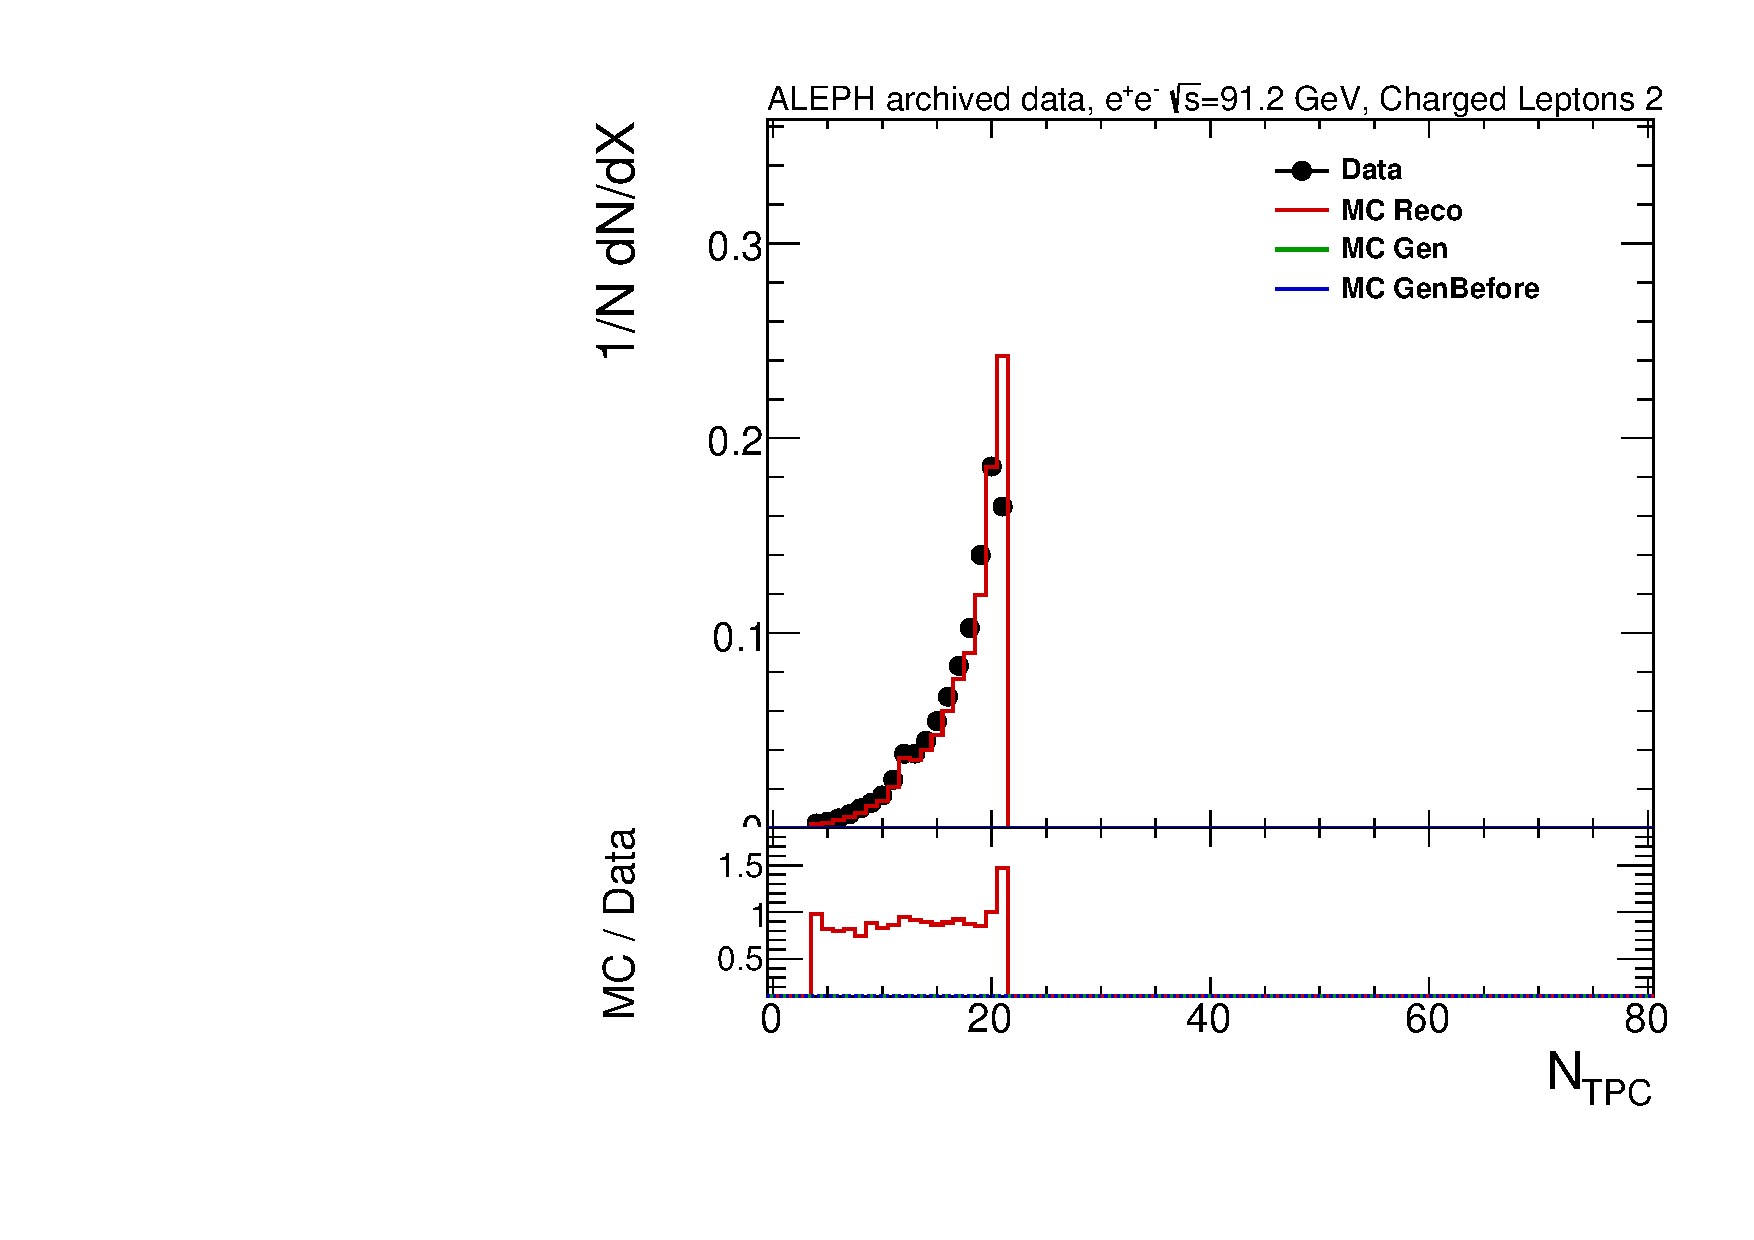
\includegraphics[width=0.242\textwidth]{figures/pwflag2_ntpc.pdf}
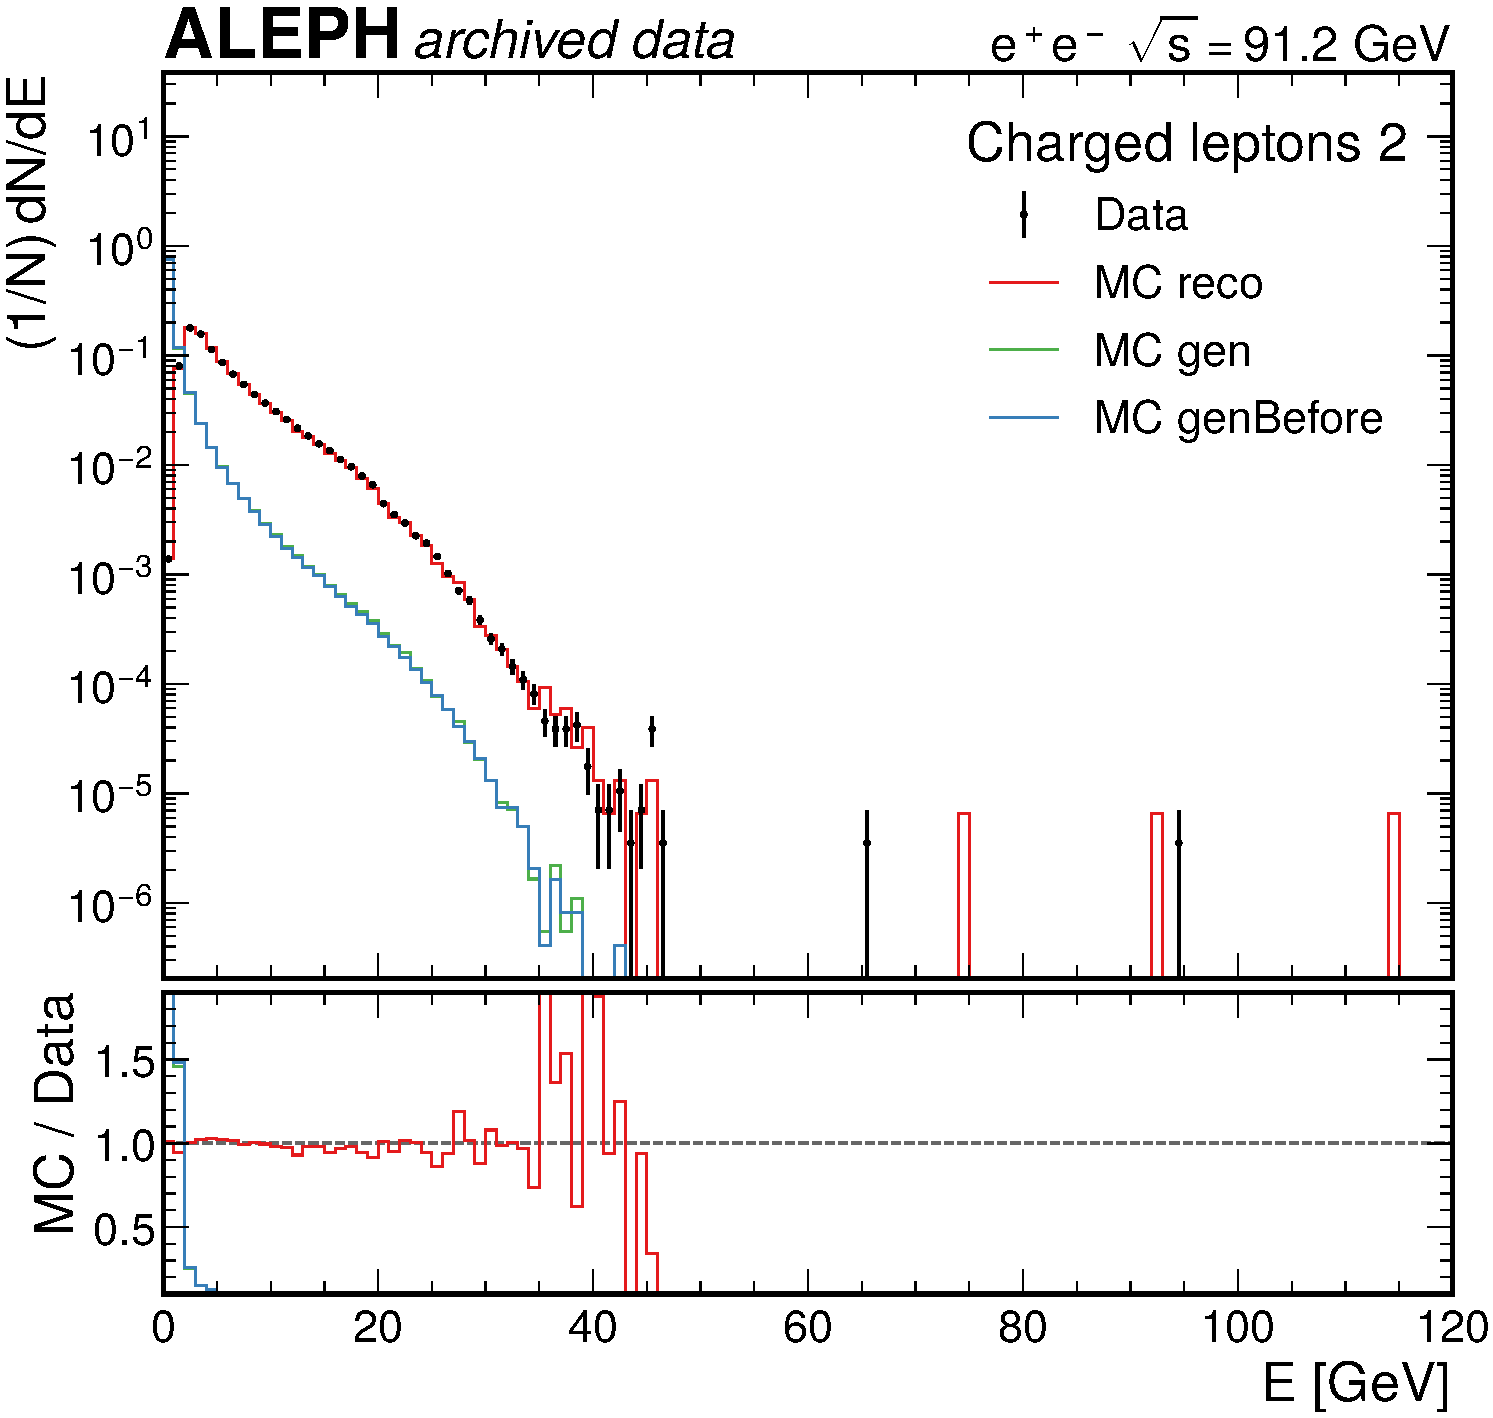
\includegraphics[width=0.242\textwidth]{figures/pwflag2_energy.pdf}
% 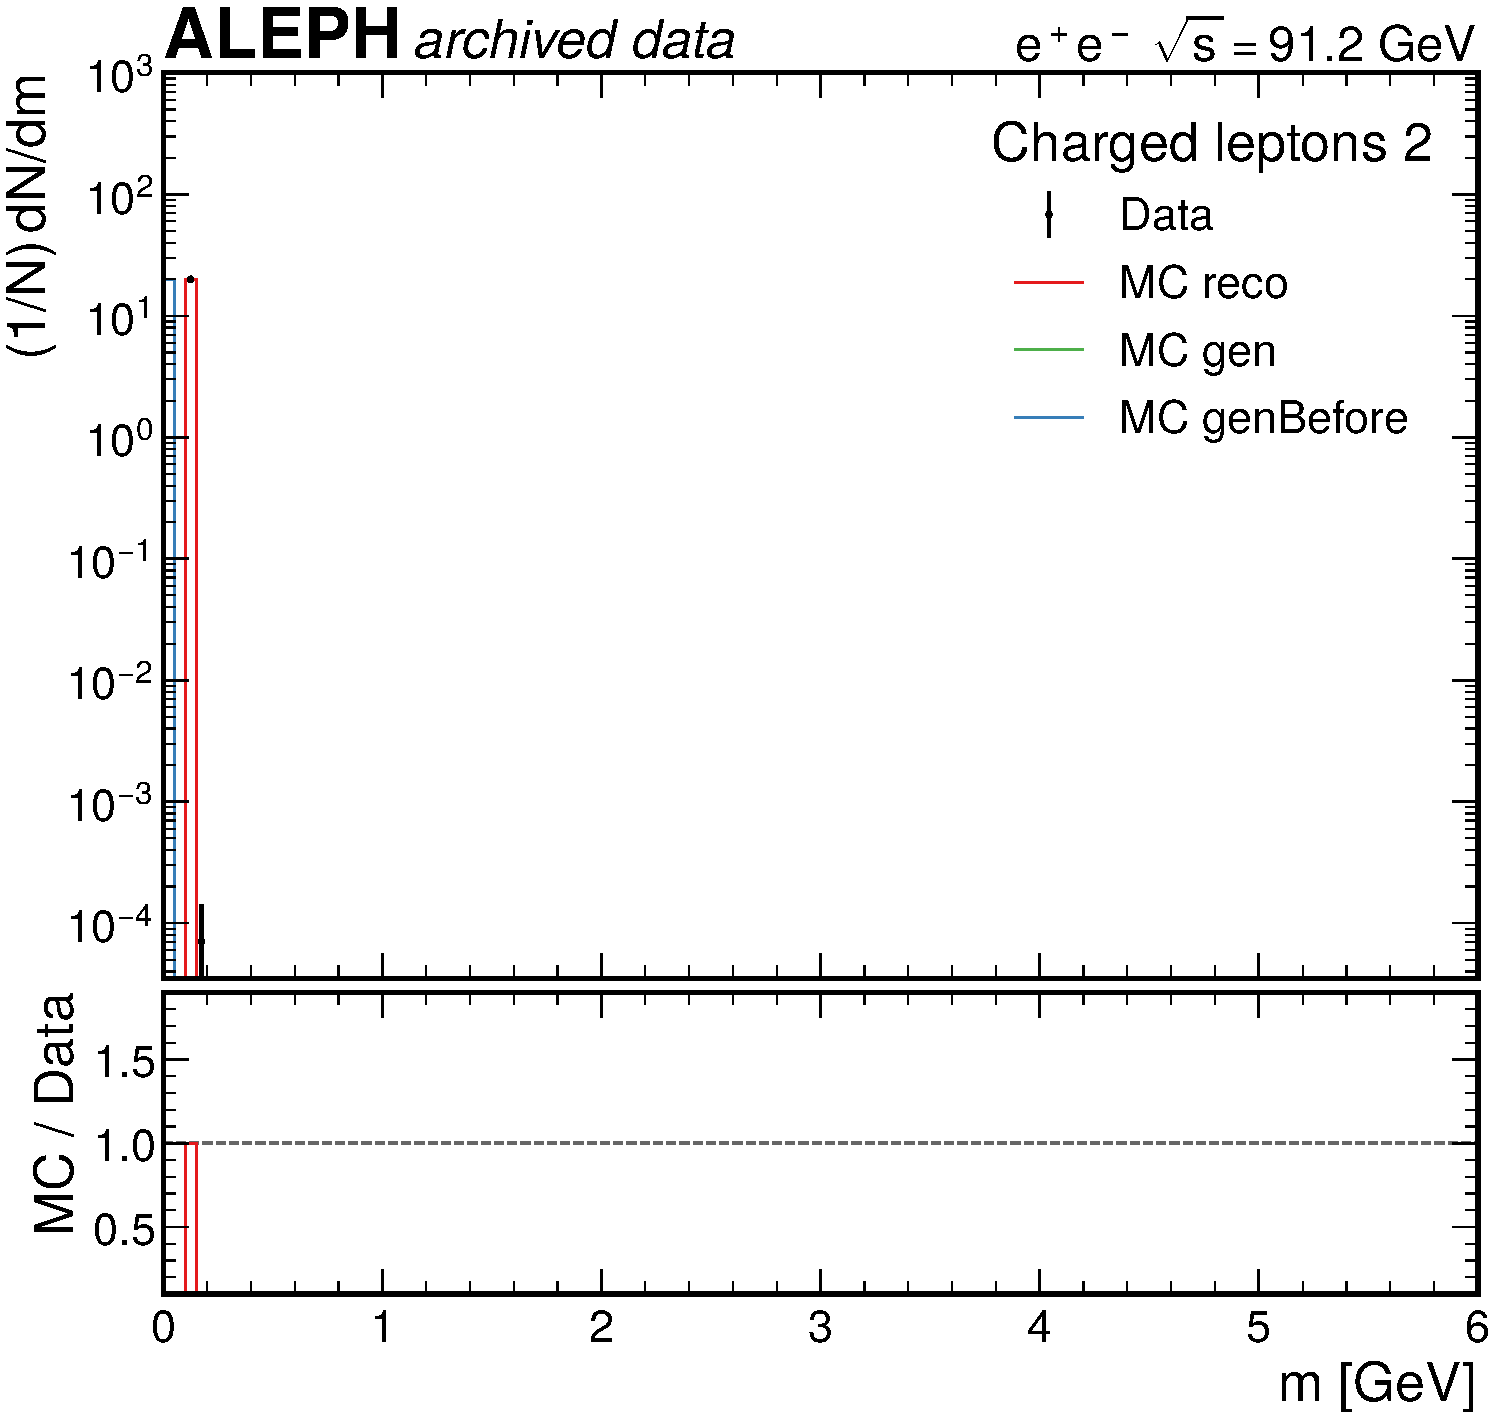
\includegraphics[width=0.242\textwidth]{figures/pwflag2_mass.pdf}
\caption{Complete \texttt{pwflag}=2 kinematic set.}
\label{fig:pwflag2_full}
\end{figure}

\begin{figure}[t!]
\centering
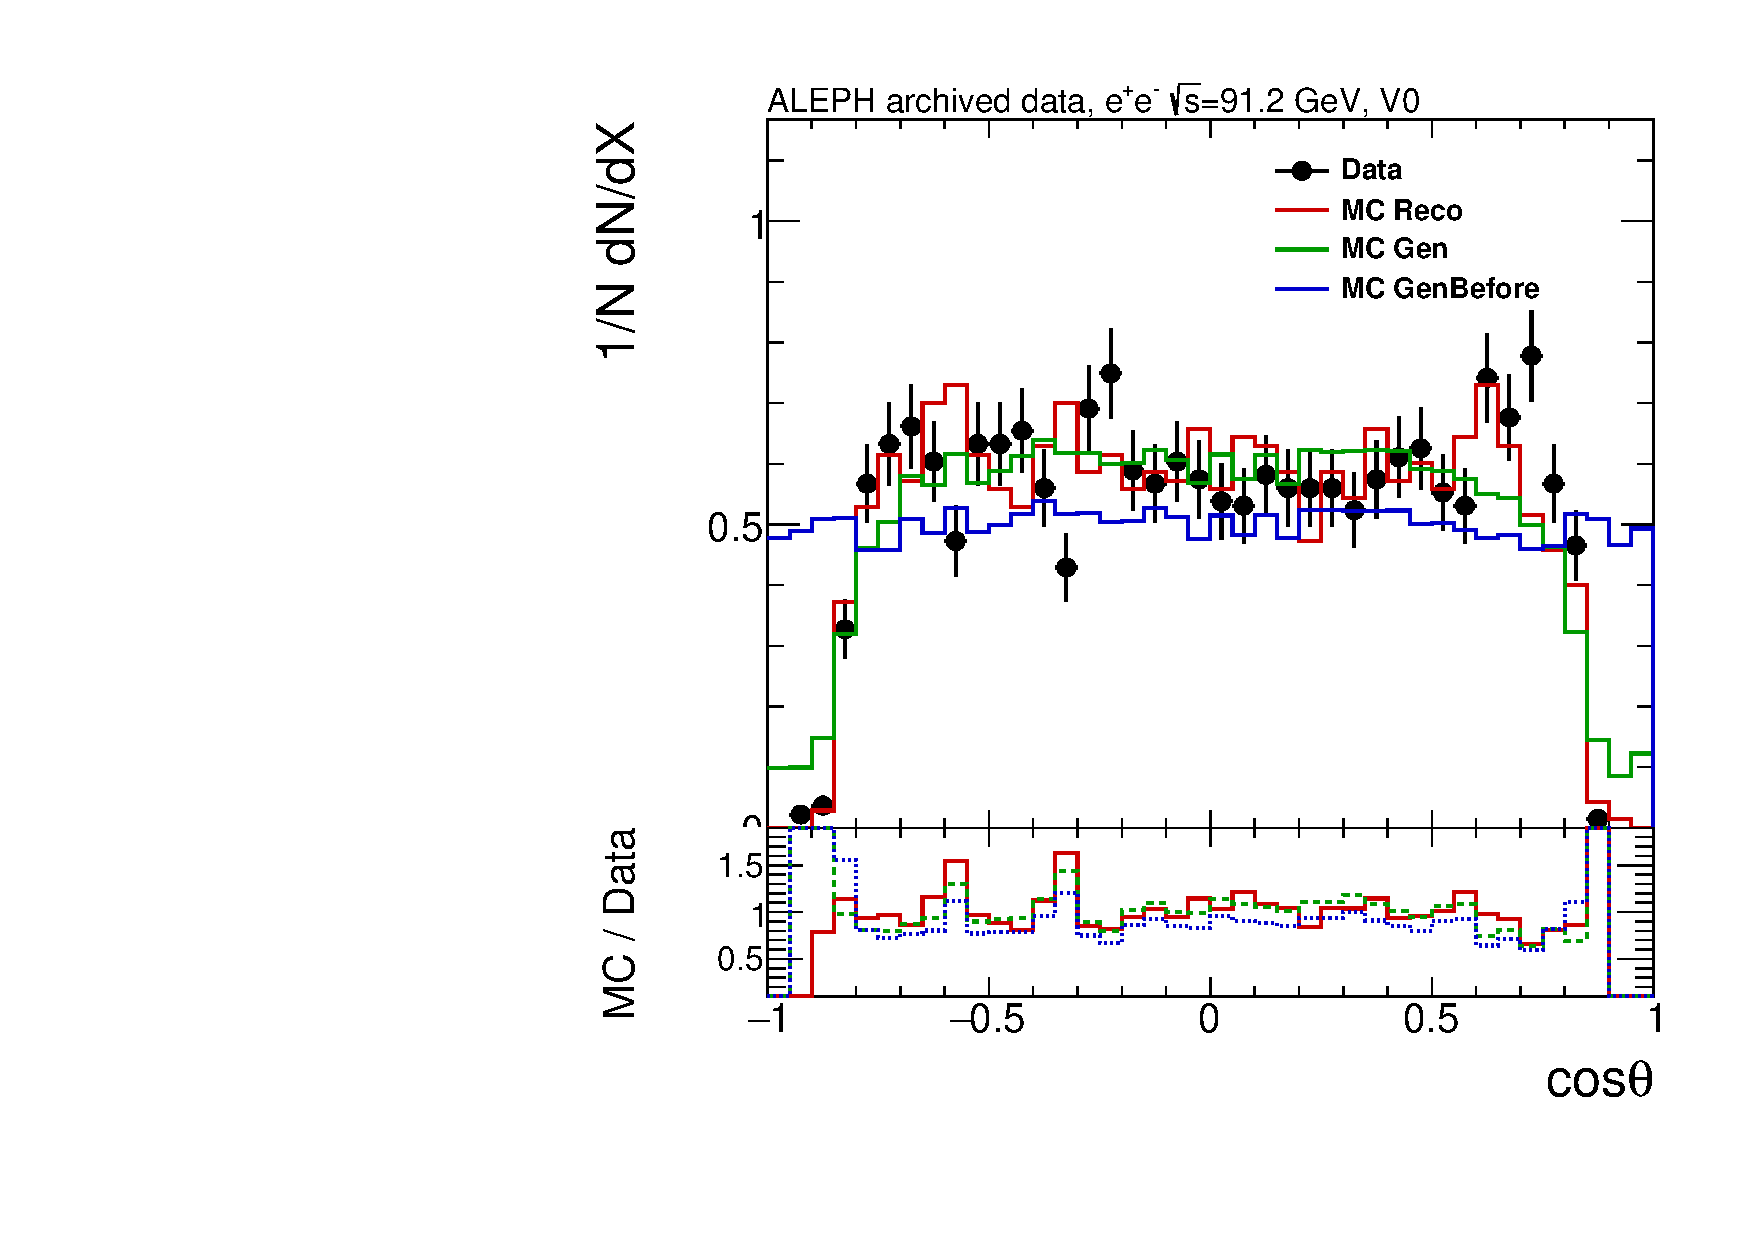
\includegraphics[width=0.495\textwidth]{figures/pwflag3_cosTheta.pdf}
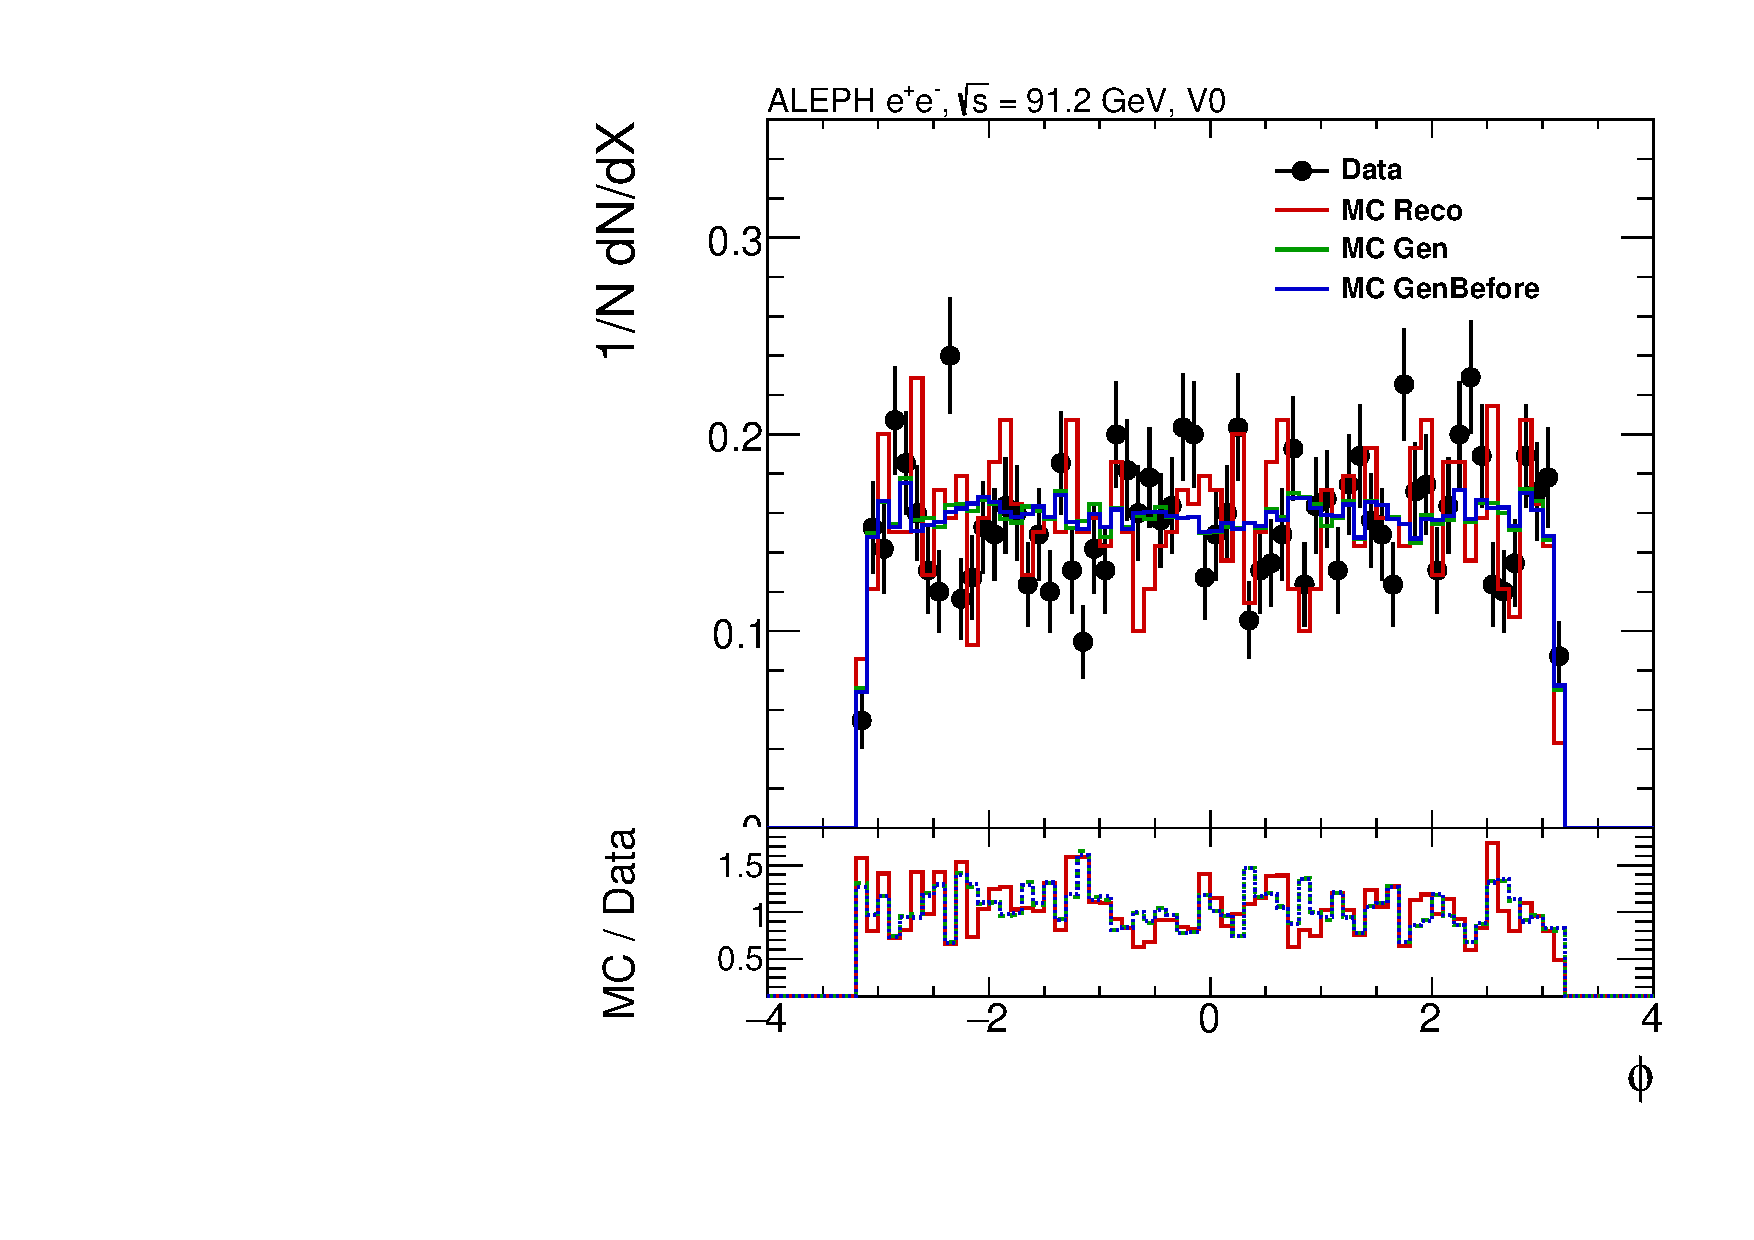
\includegraphics[width=0.495\textwidth]{figures/pwflag3_phi.pdf}
% 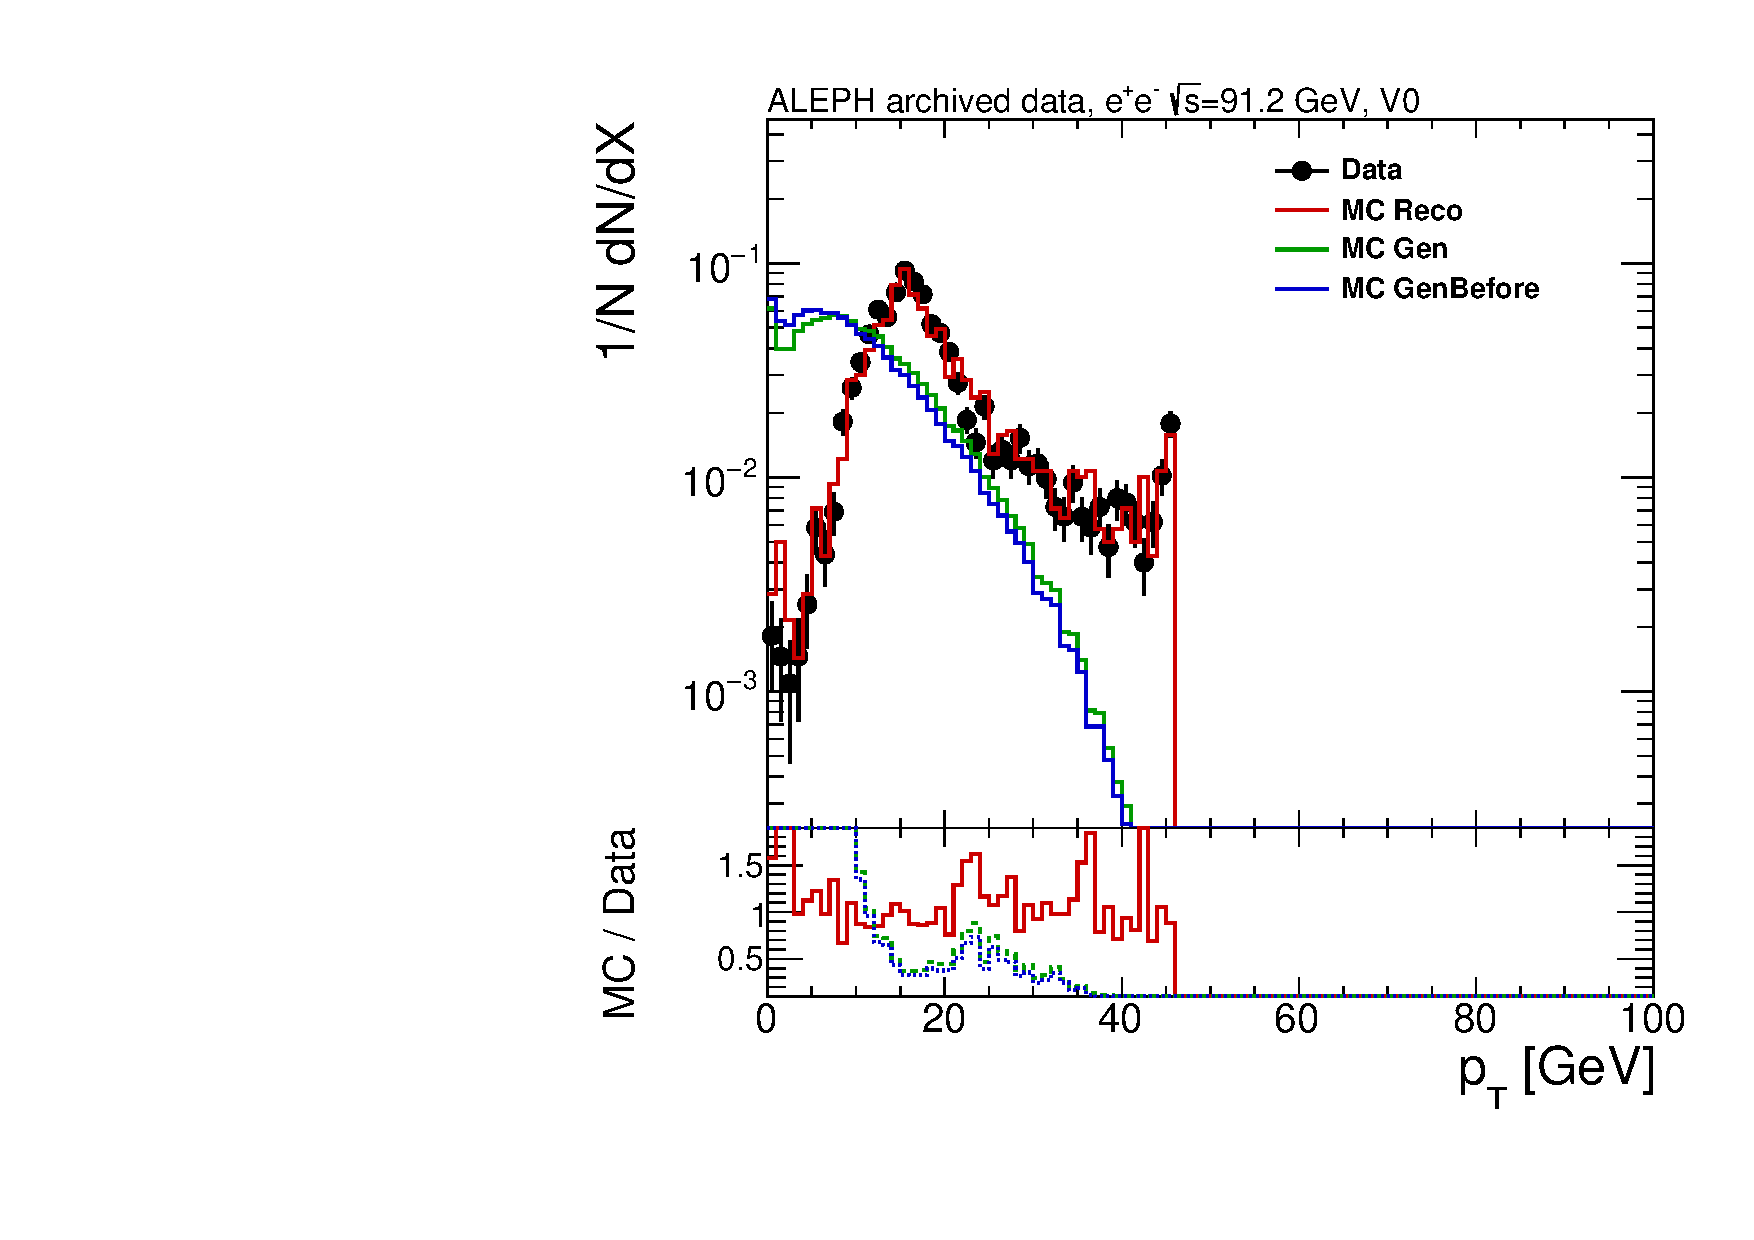
\includegraphics[width=0.242\textwidth]{figures/pwflag3_pt.pdf}
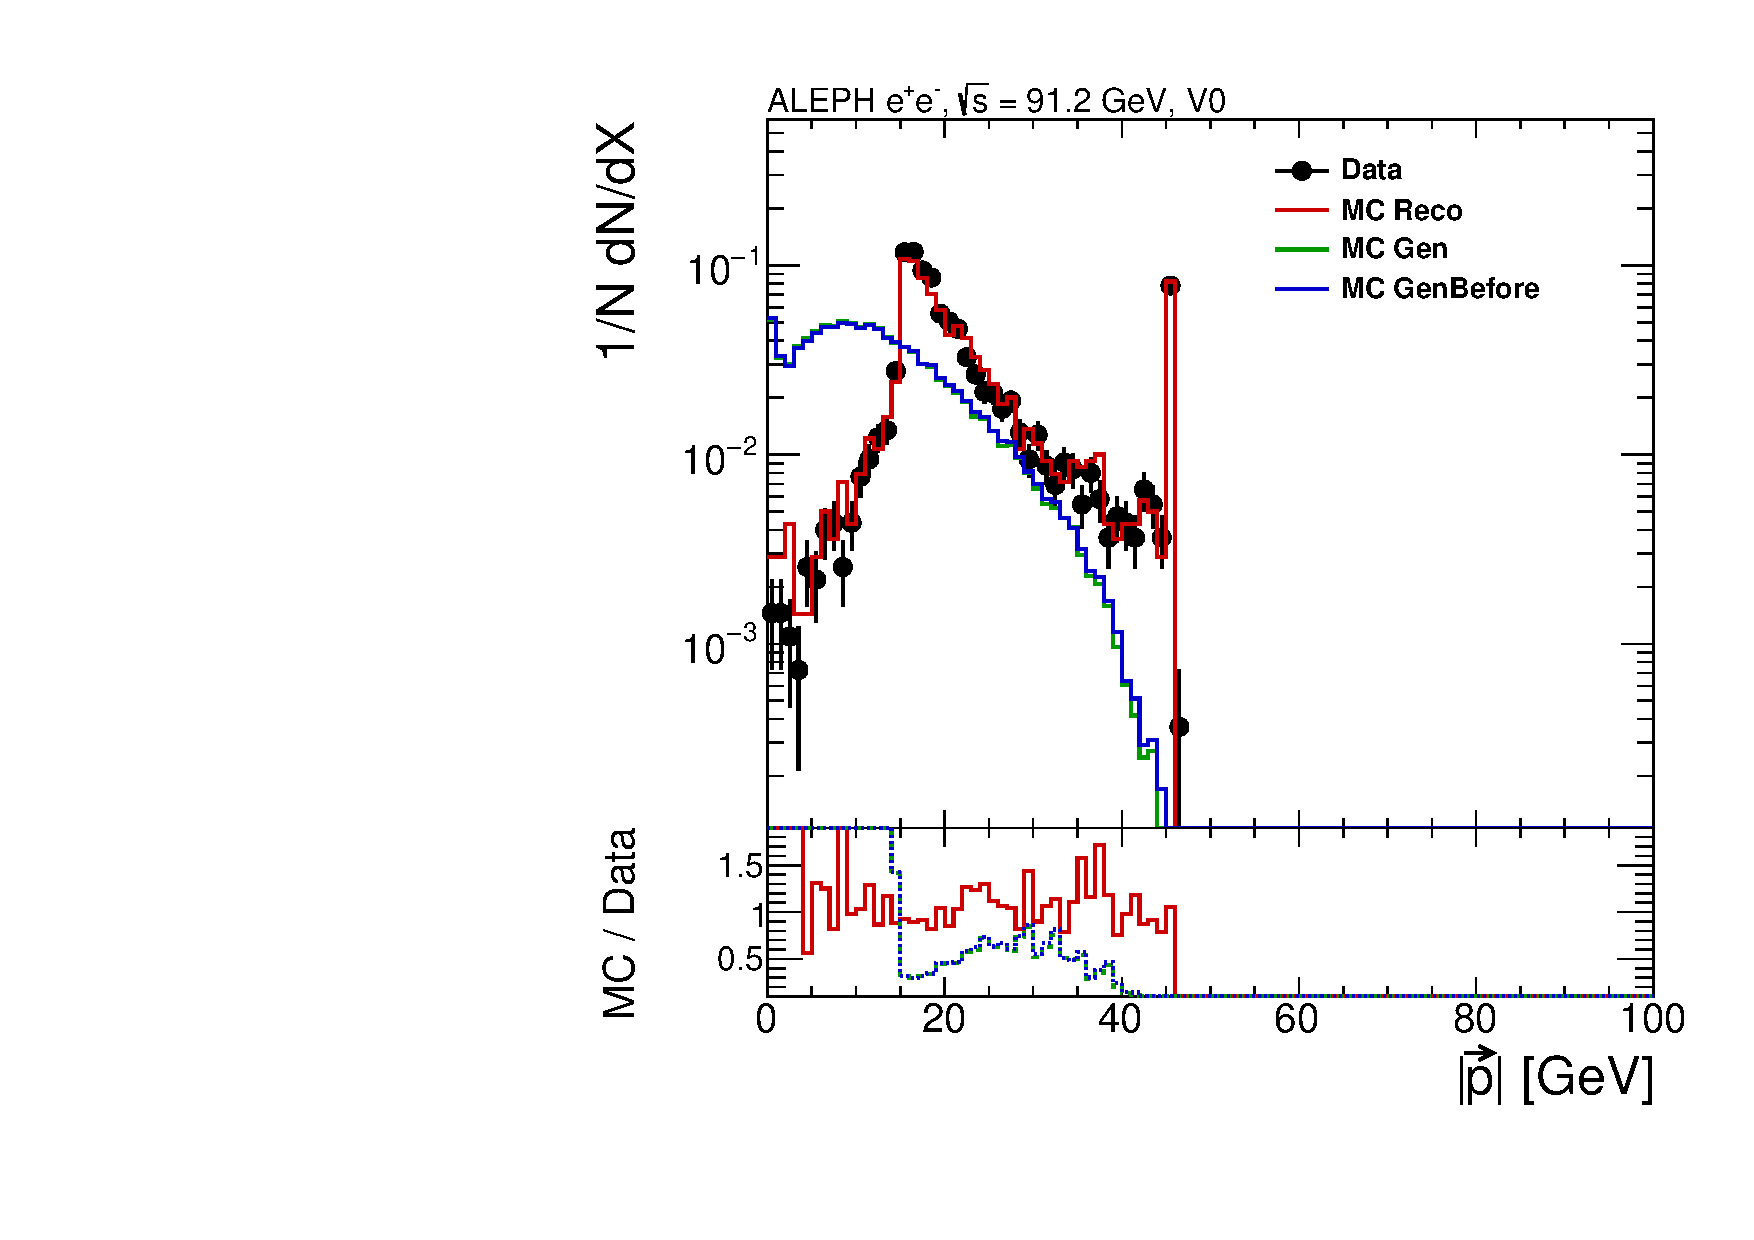
\includegraphics[width=0.495\textwidth]{figures/pwflag3_pmag.pdf}
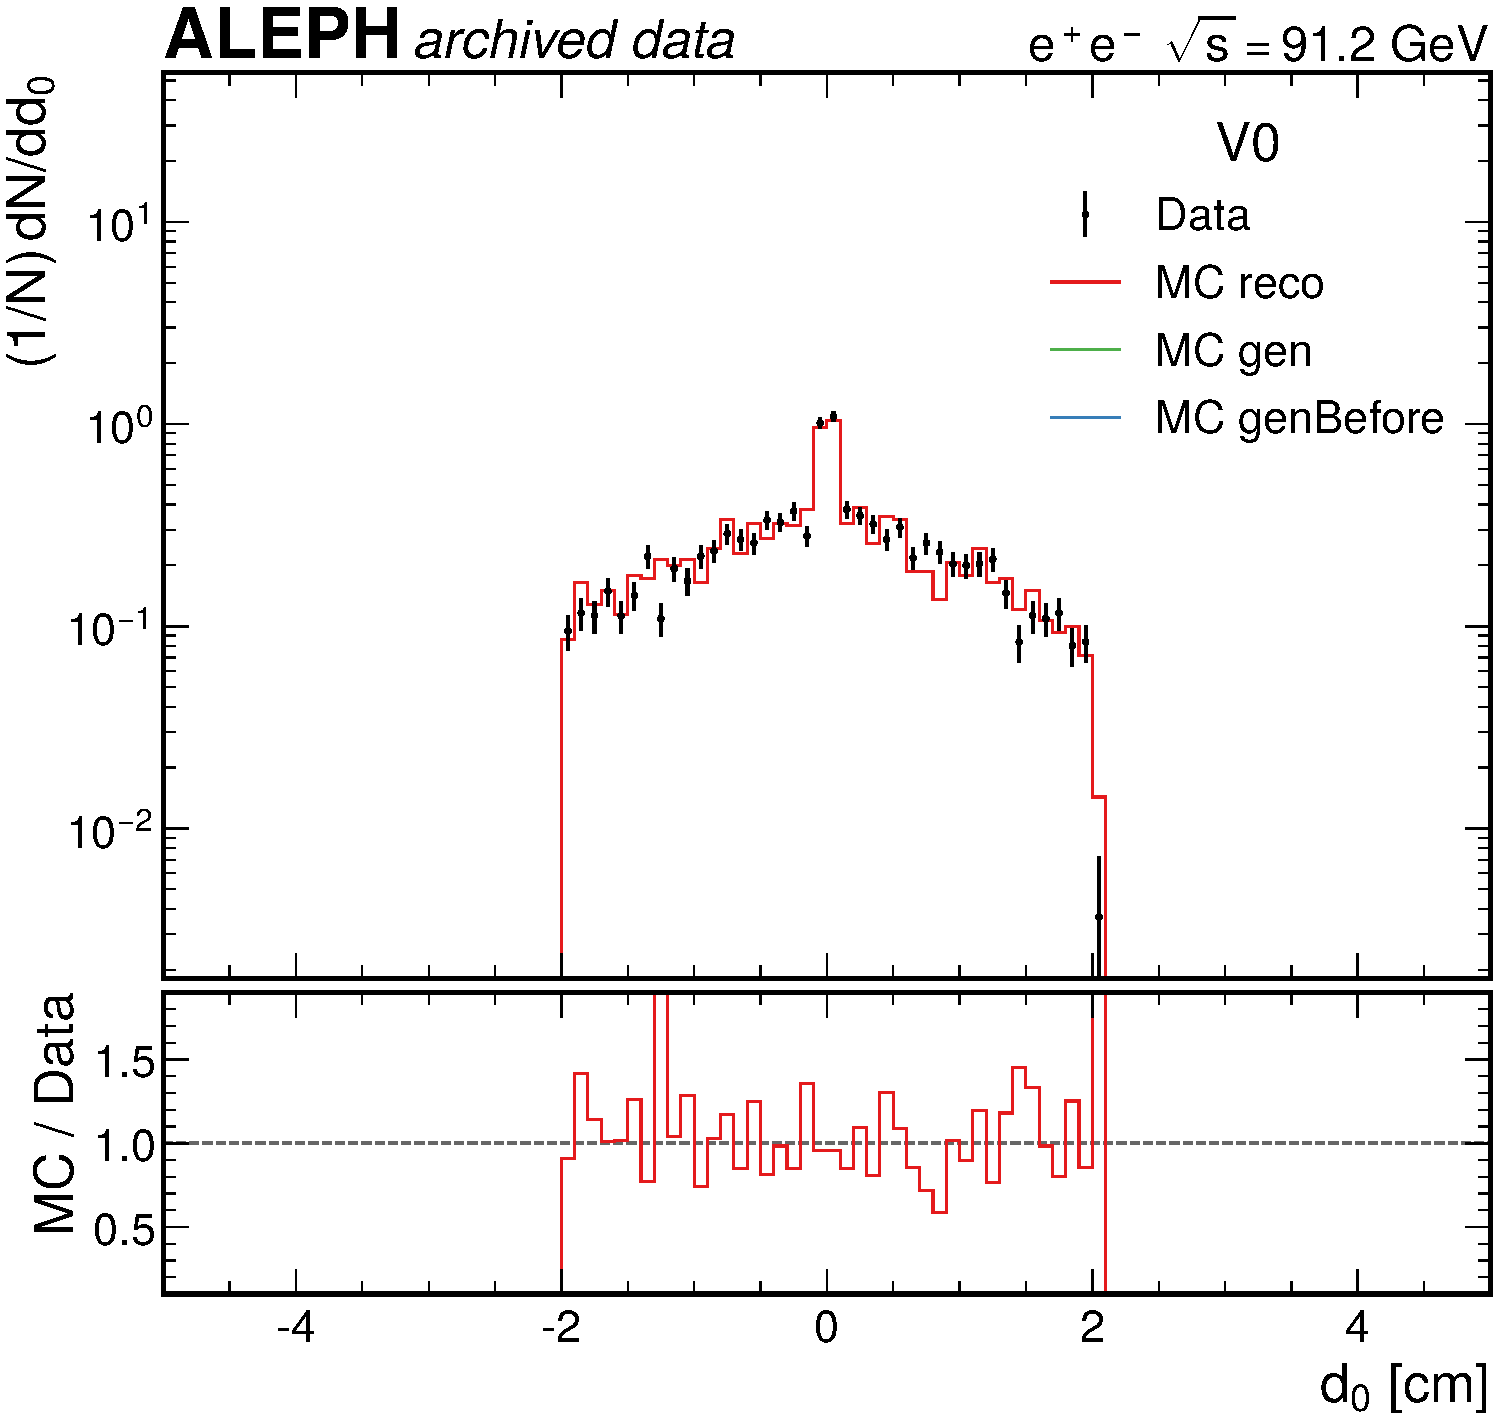
\includegraphics[width=0.495\textwidth]{figures/pwflag3_d0.pdf}
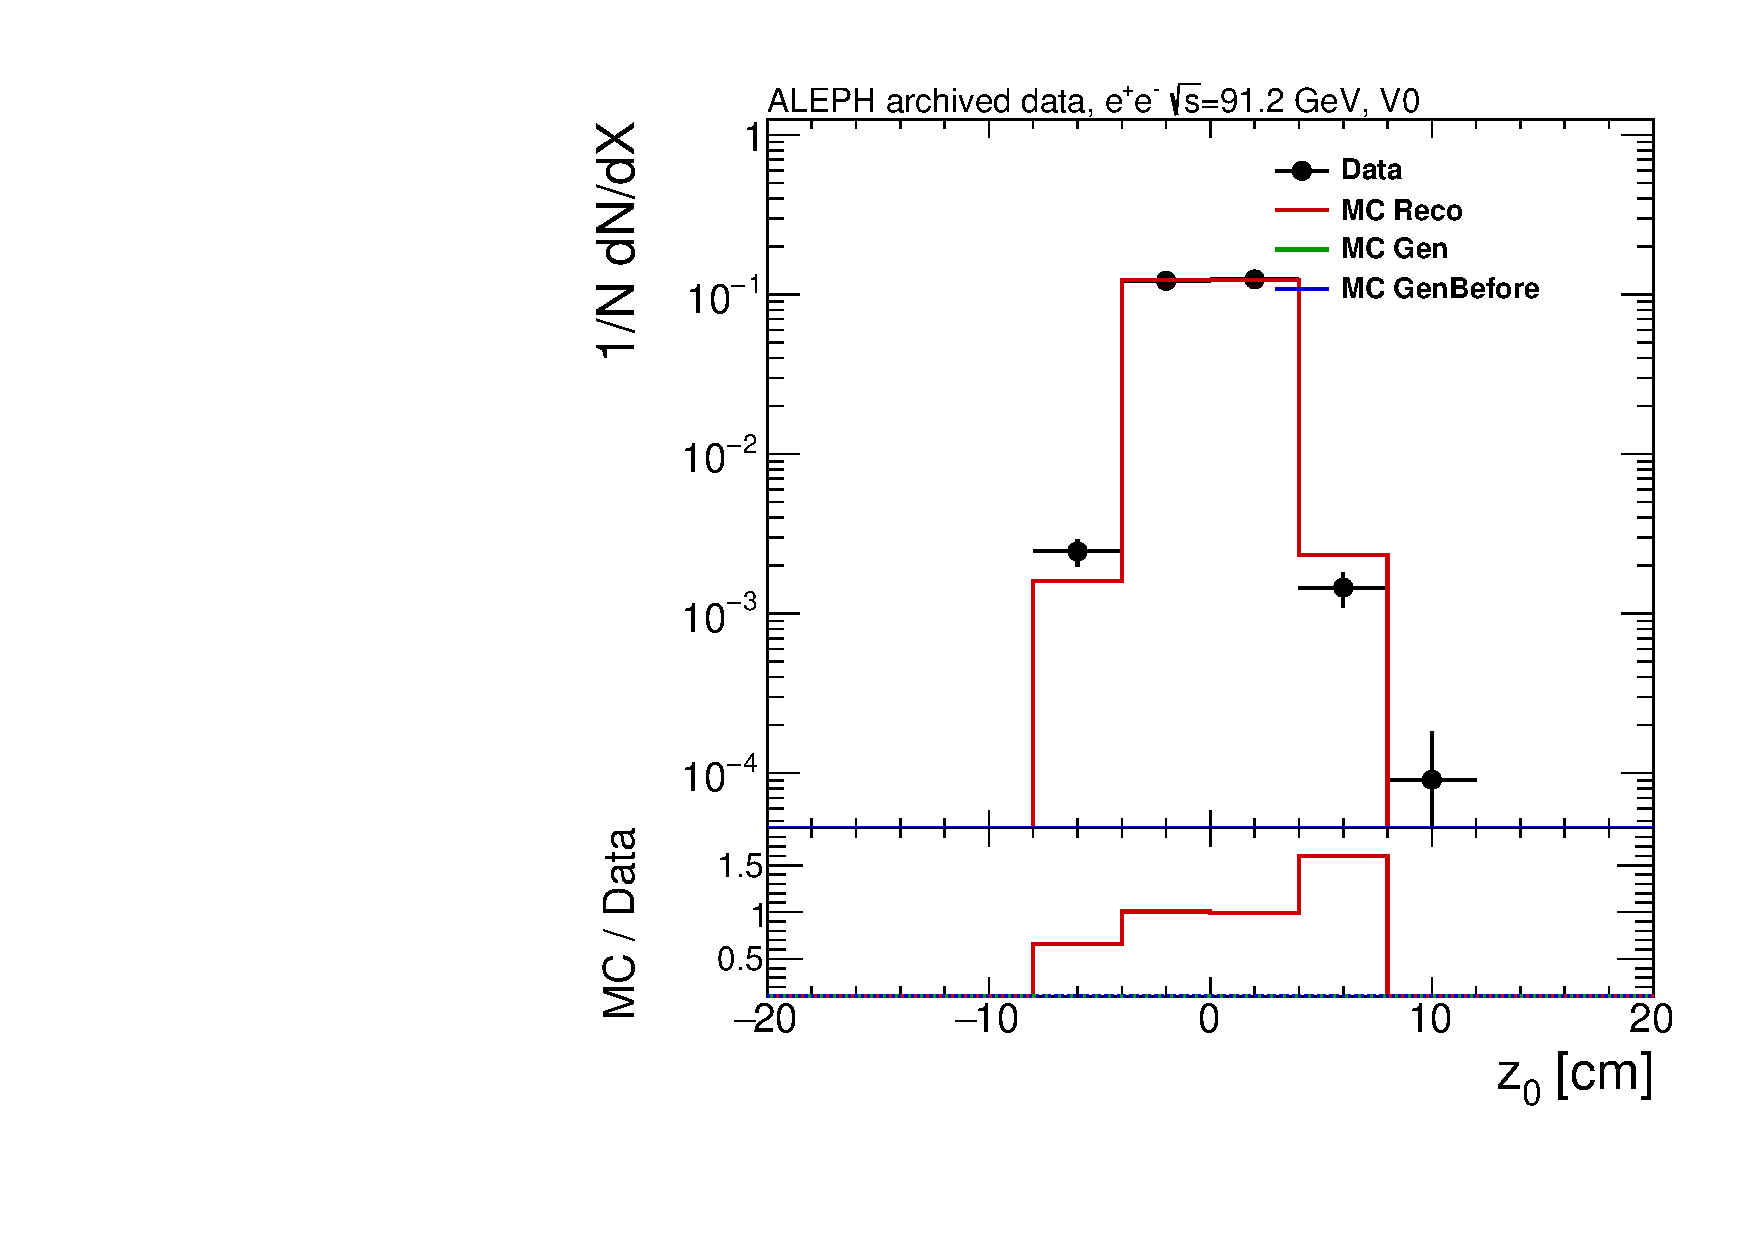
\includegraphics[width=0.495\textwidth]{figures/pwflag3_z0.pdf}
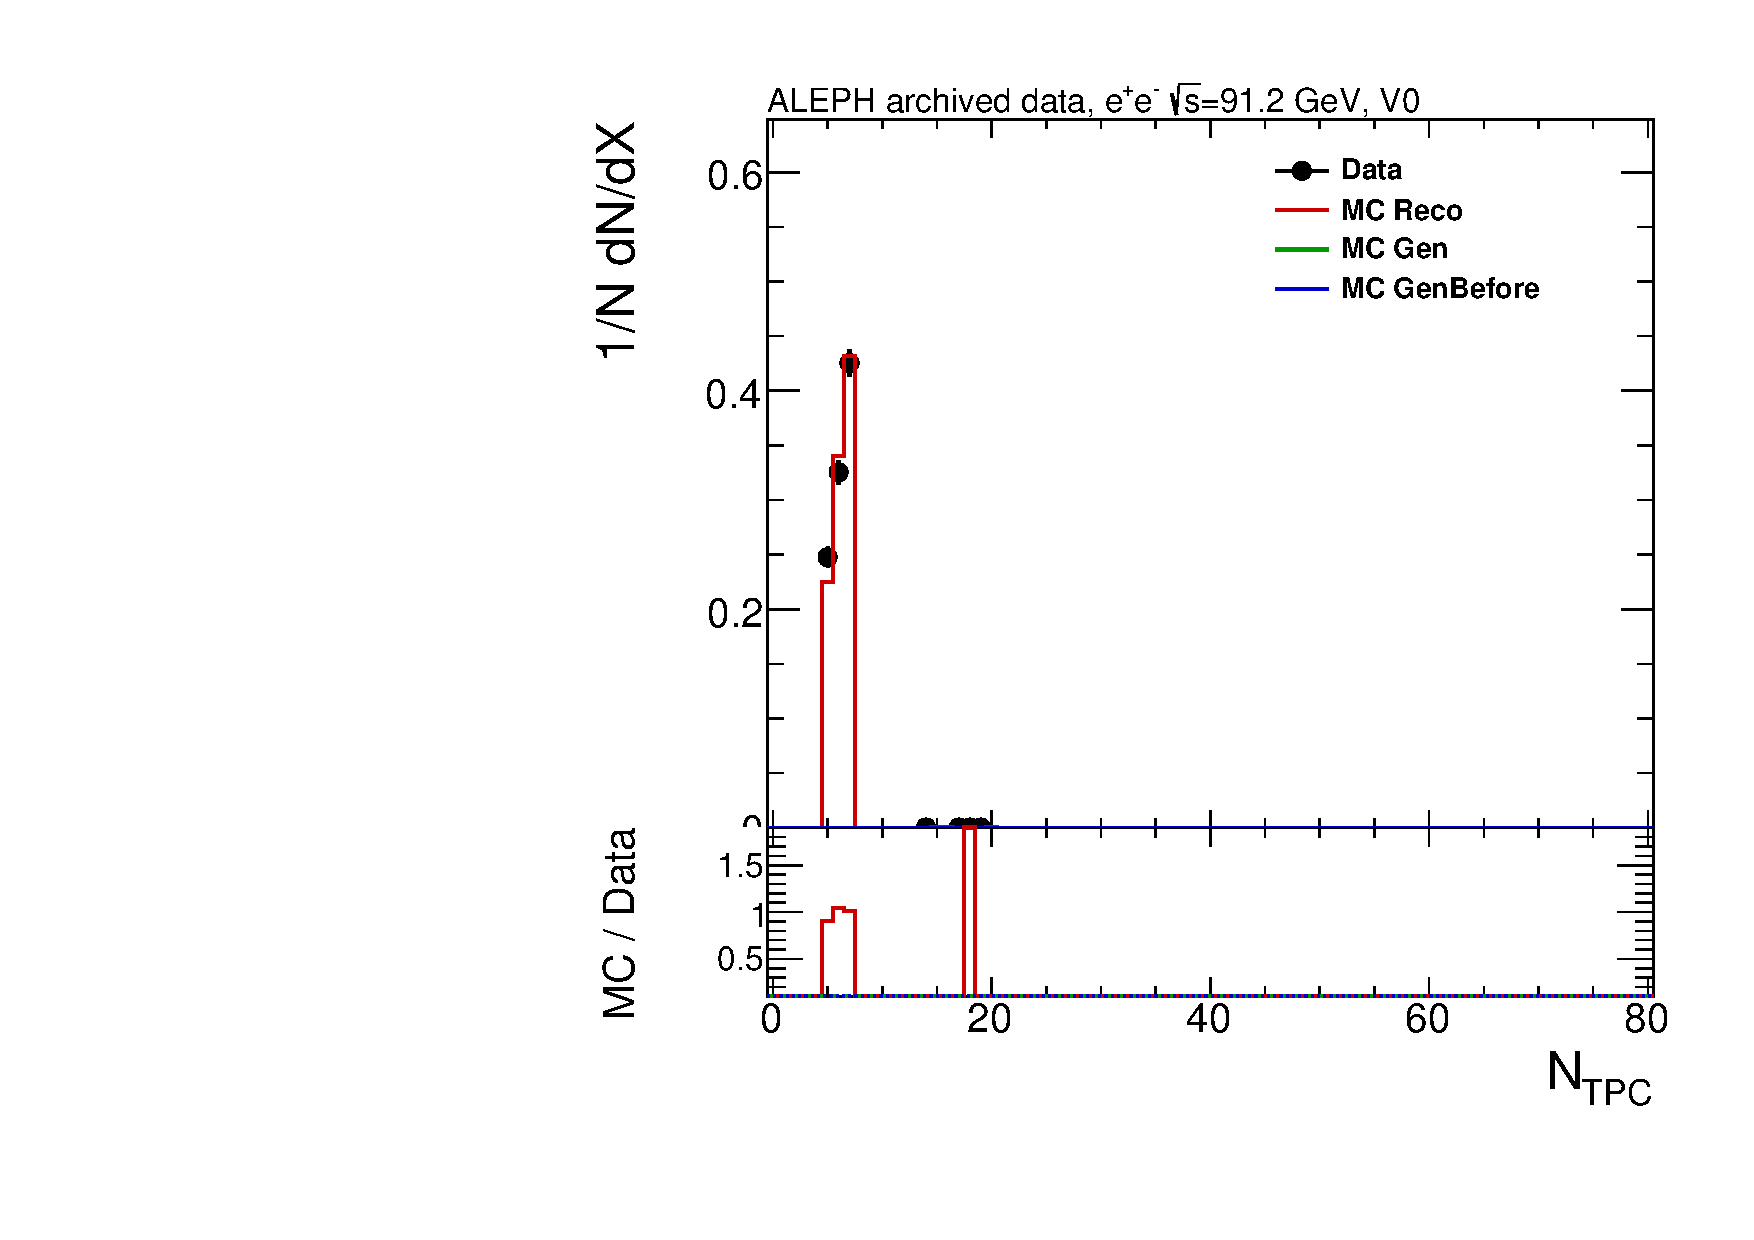
\includegraphics[width=0.495\textwidth]{figures/pwflag3_ntpc.pdf}
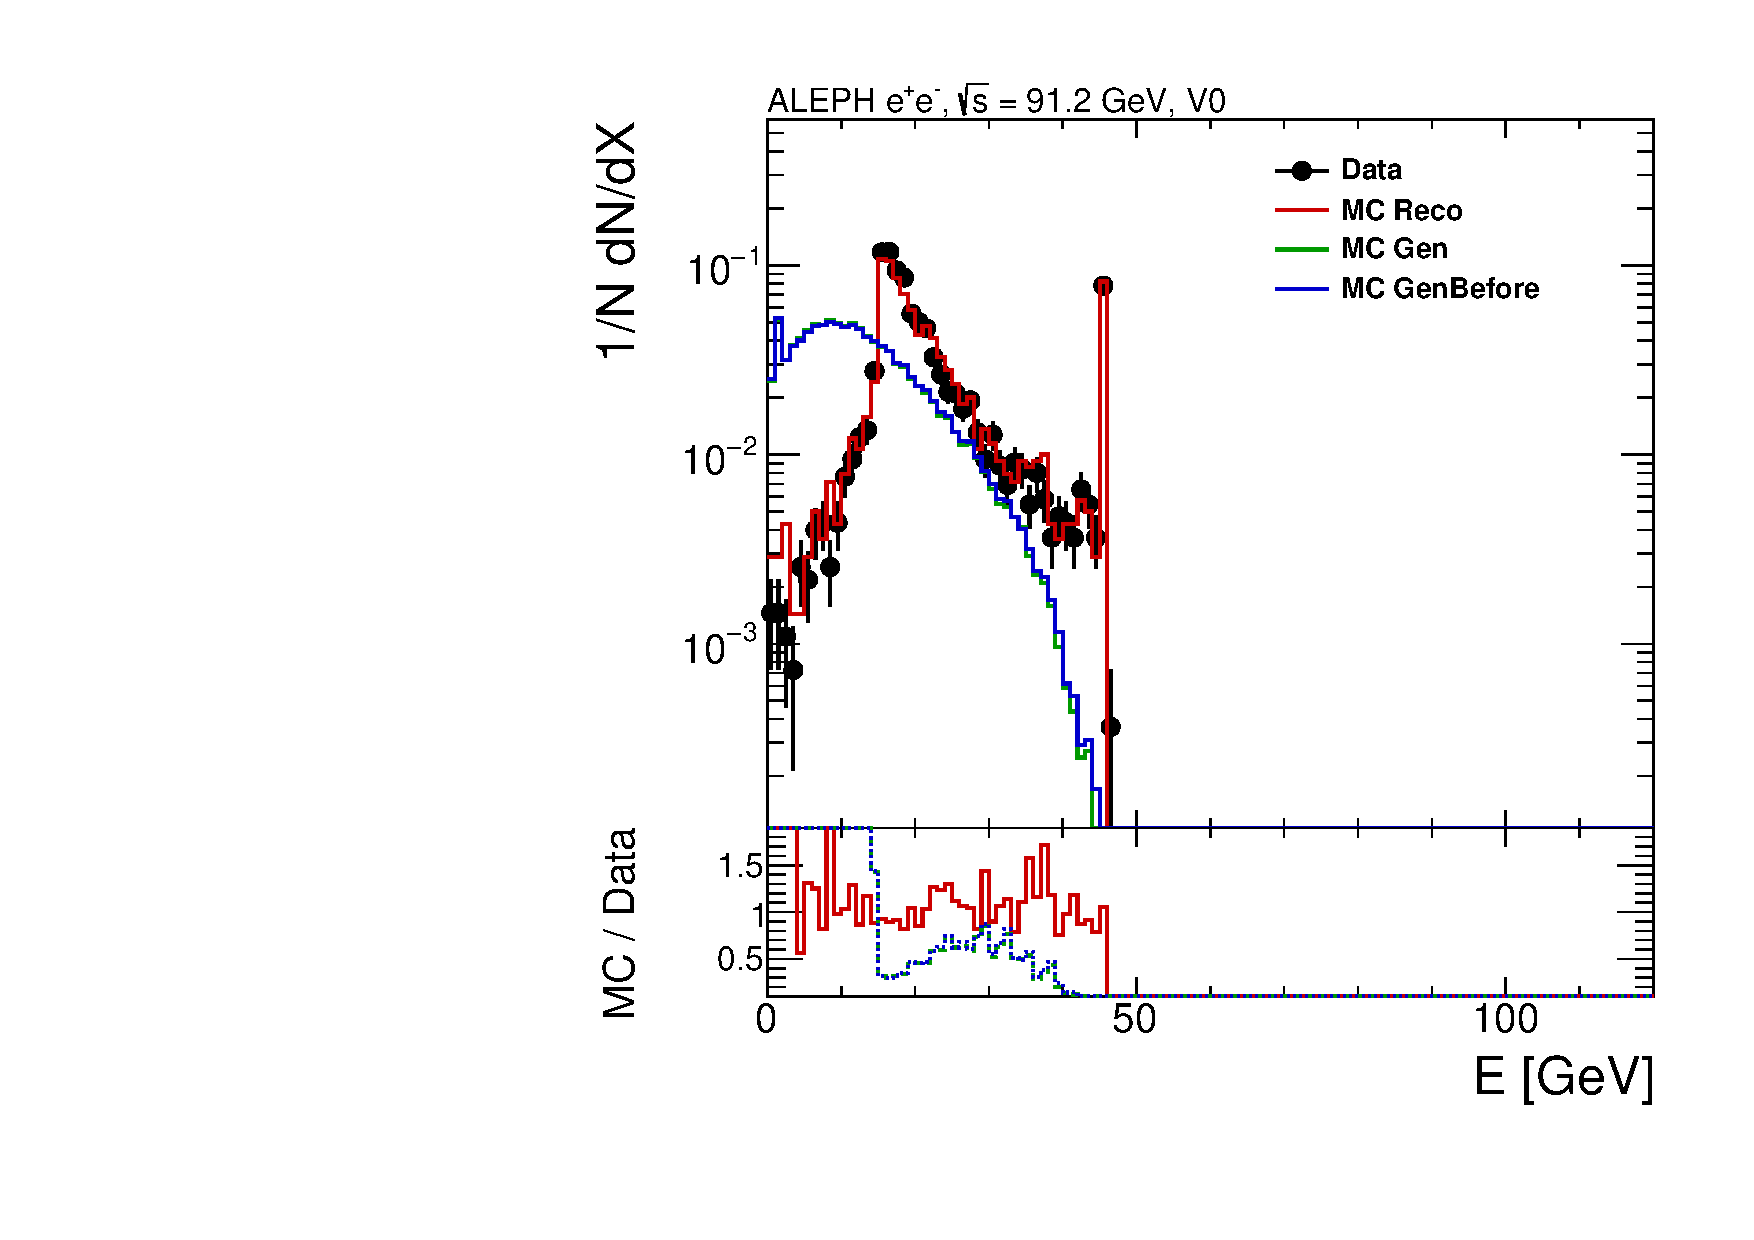
\includegraphics[width=0.495\textwidth]{figures/pwflag3_energy.pdf}
% 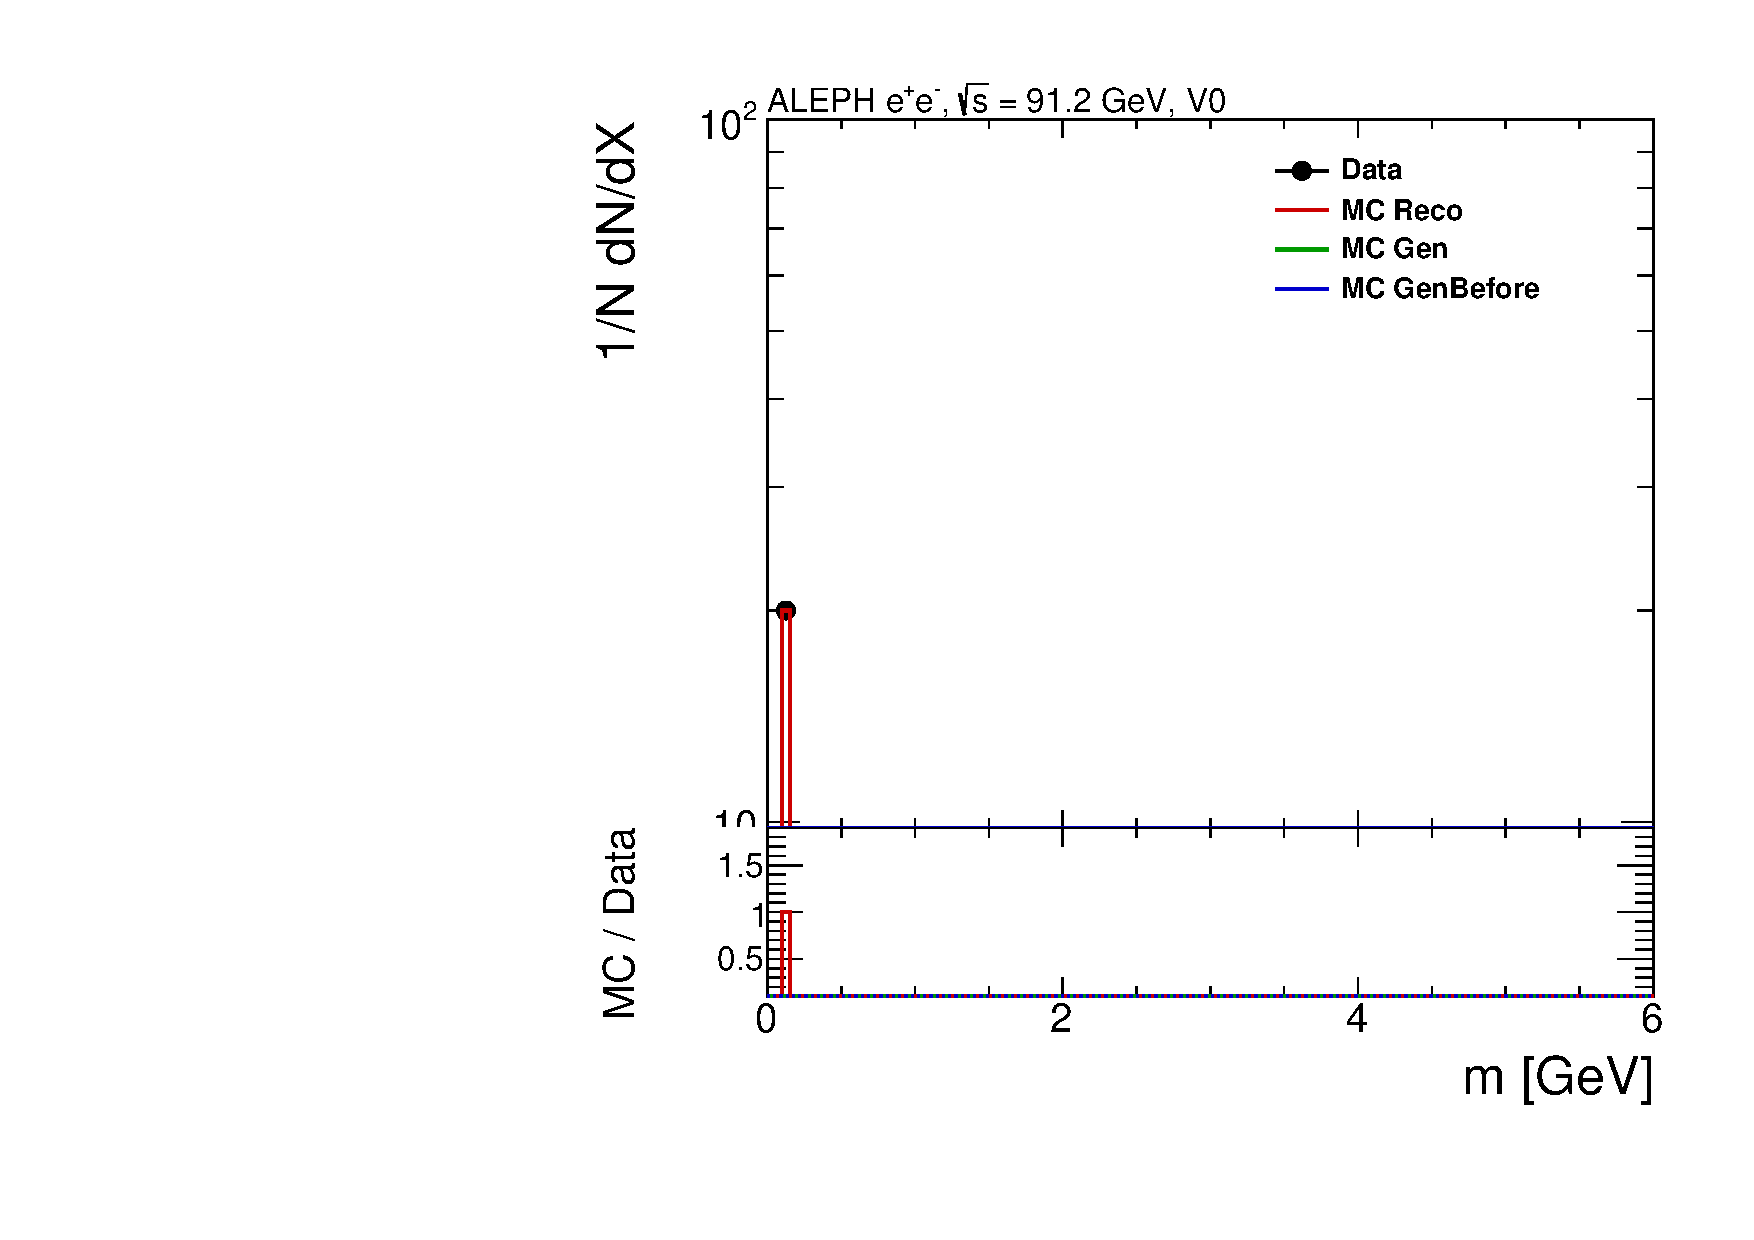
\includegraphics[width=0.242\textwidth]{figures/pwflag3_mass.pdf}
\caption{Complete \texttt{pwflag}=3 kinematic set.}
\label{fig:pwflag3_full}
\end{figure}

\begin{figure}[t!]
\centering
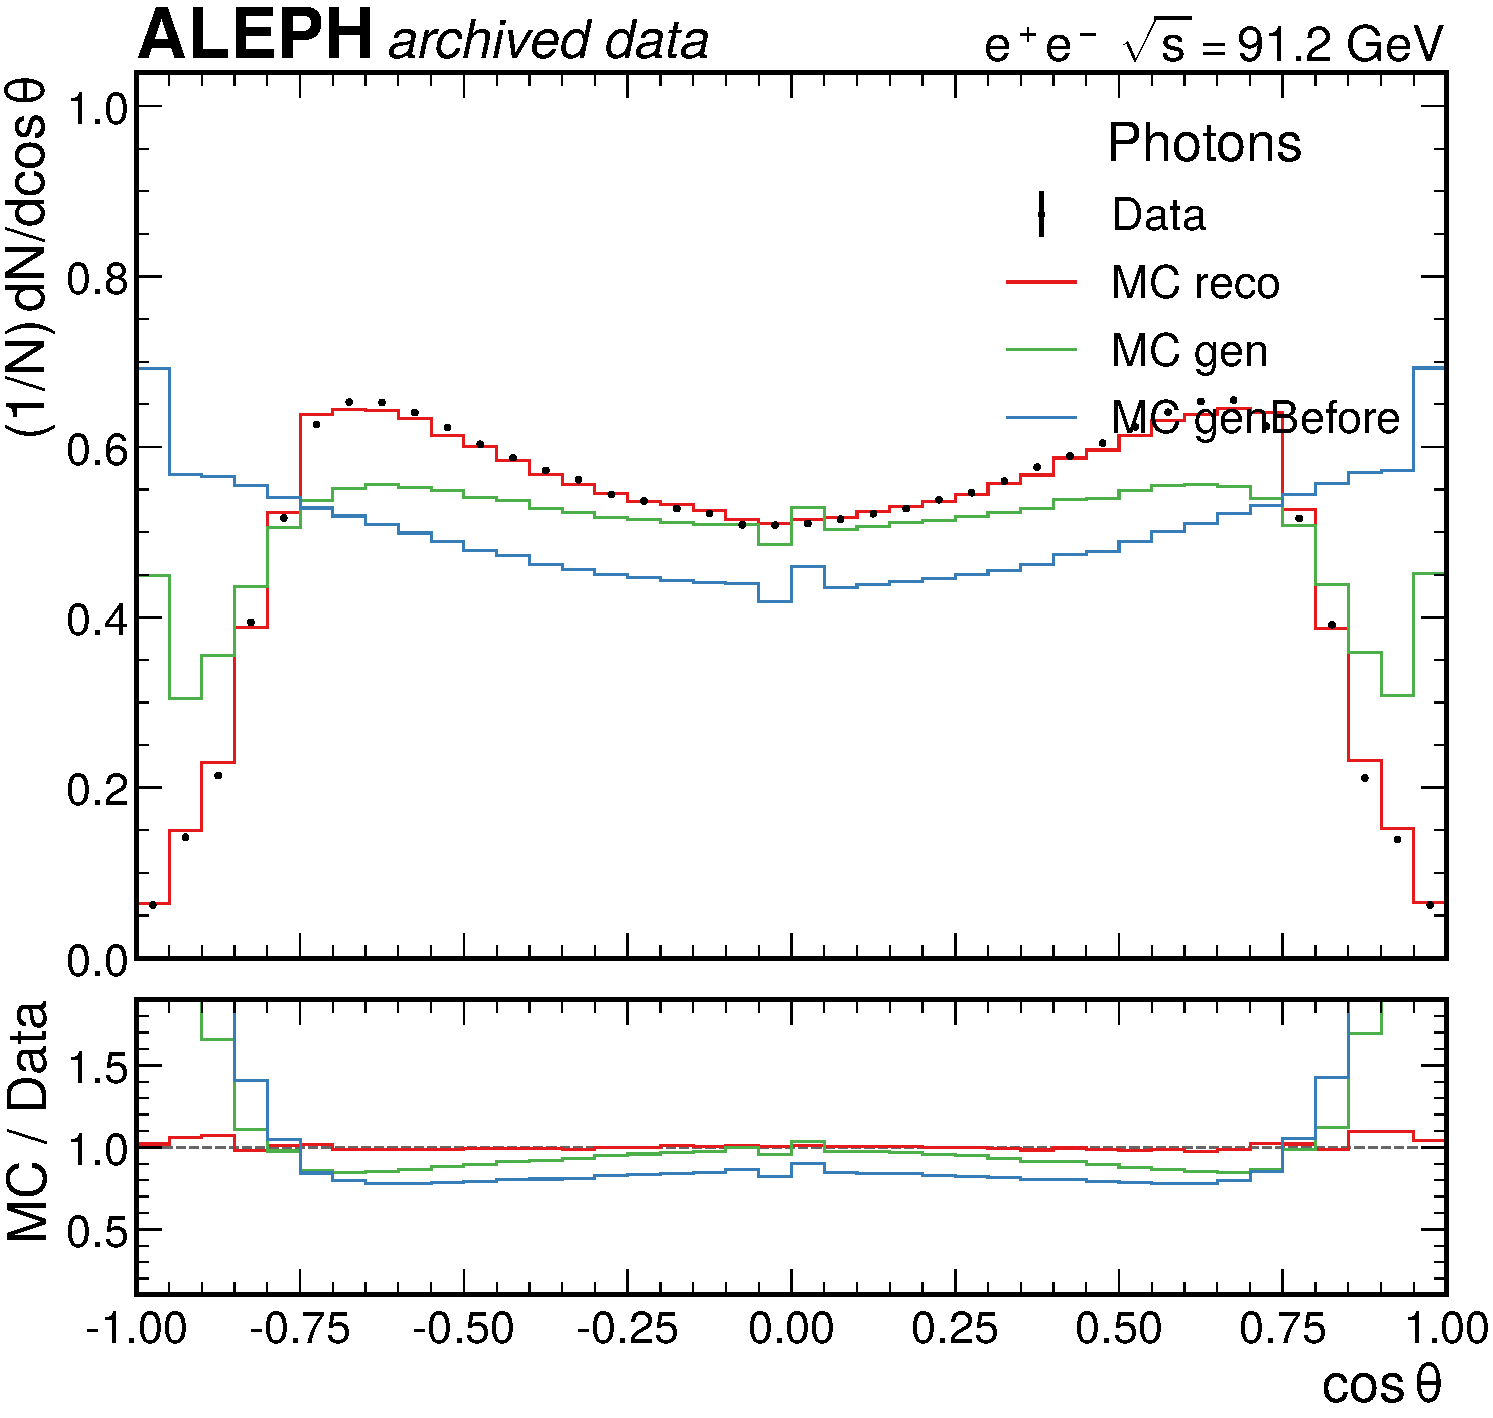
\includegraphics[width=0.495\textwidth]{figures/pwflag4_cosTheta.pdf}
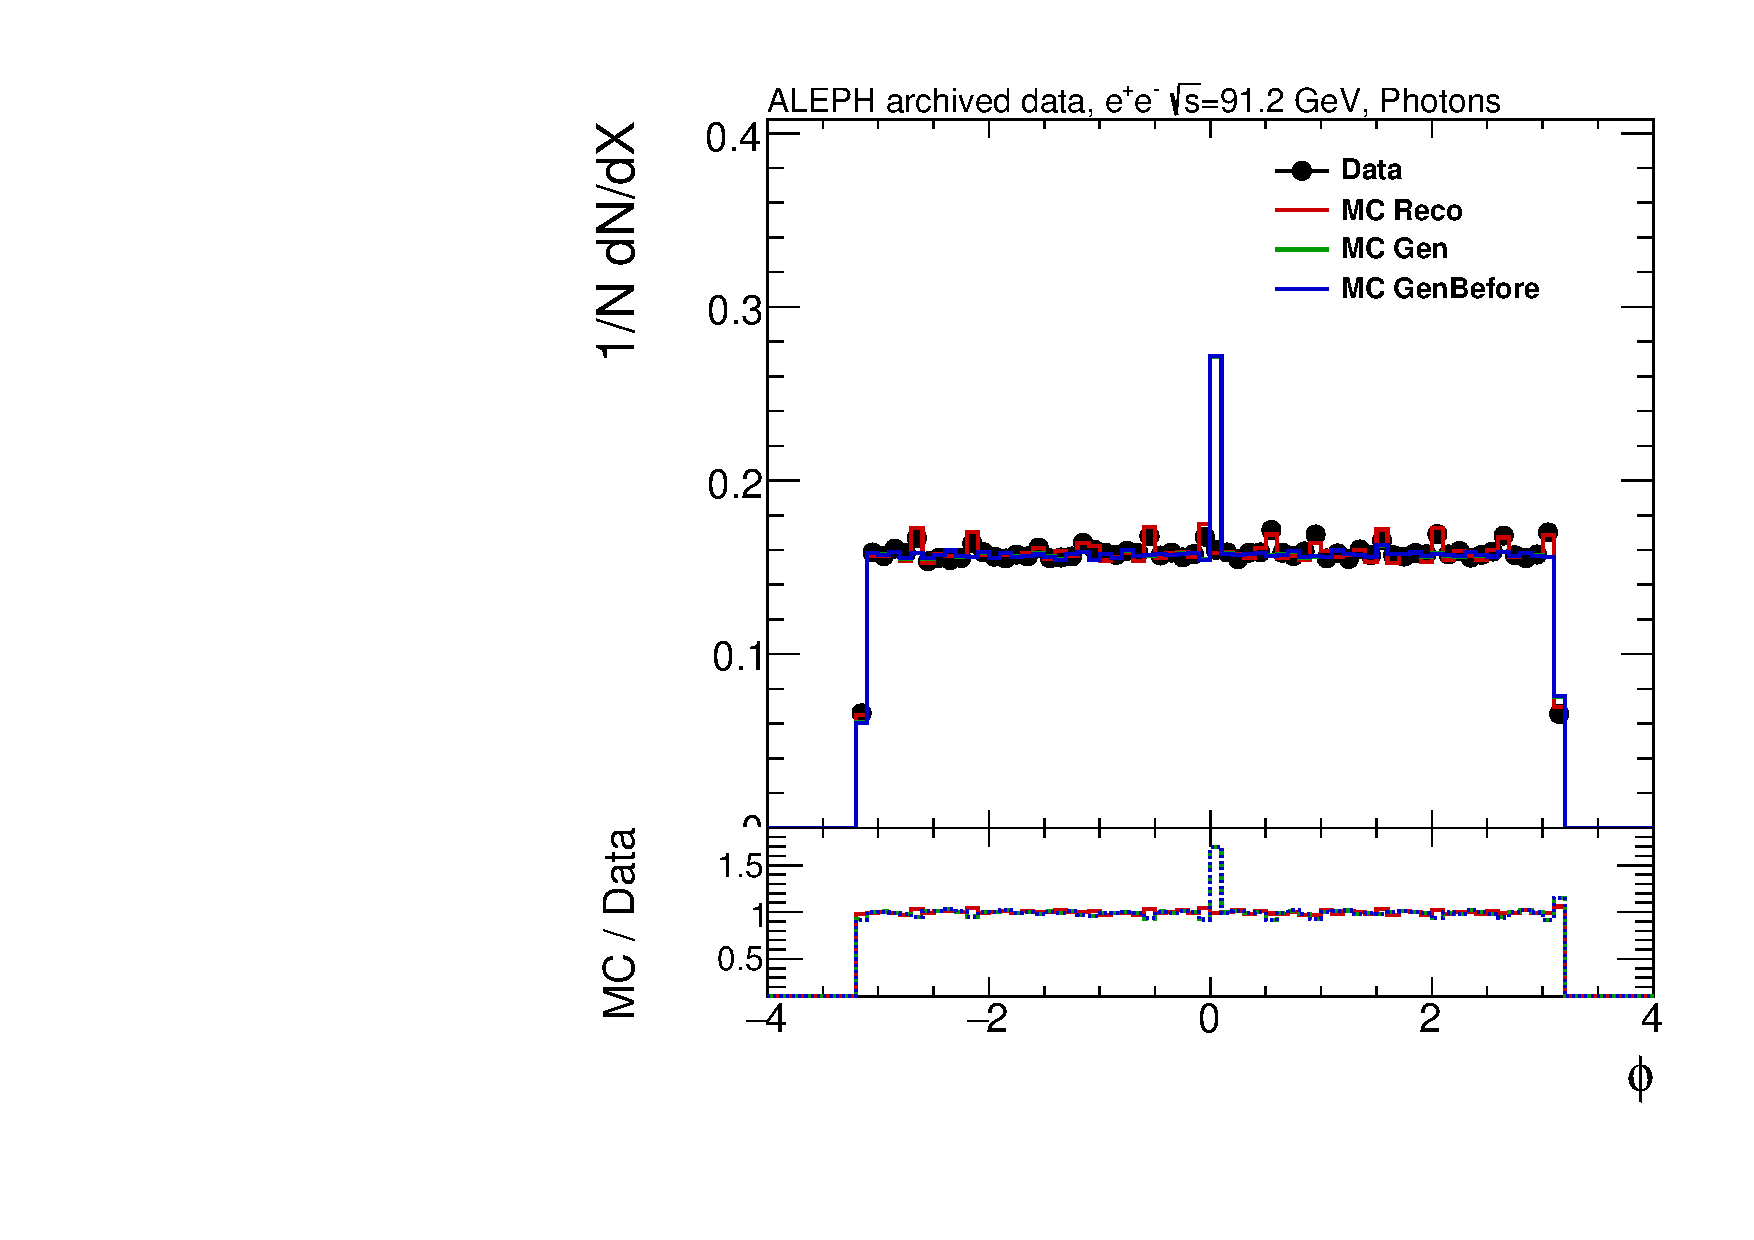
\includegraphics[width=0.495\textwidth]{figures/pwflag4_phi.pdf}
% 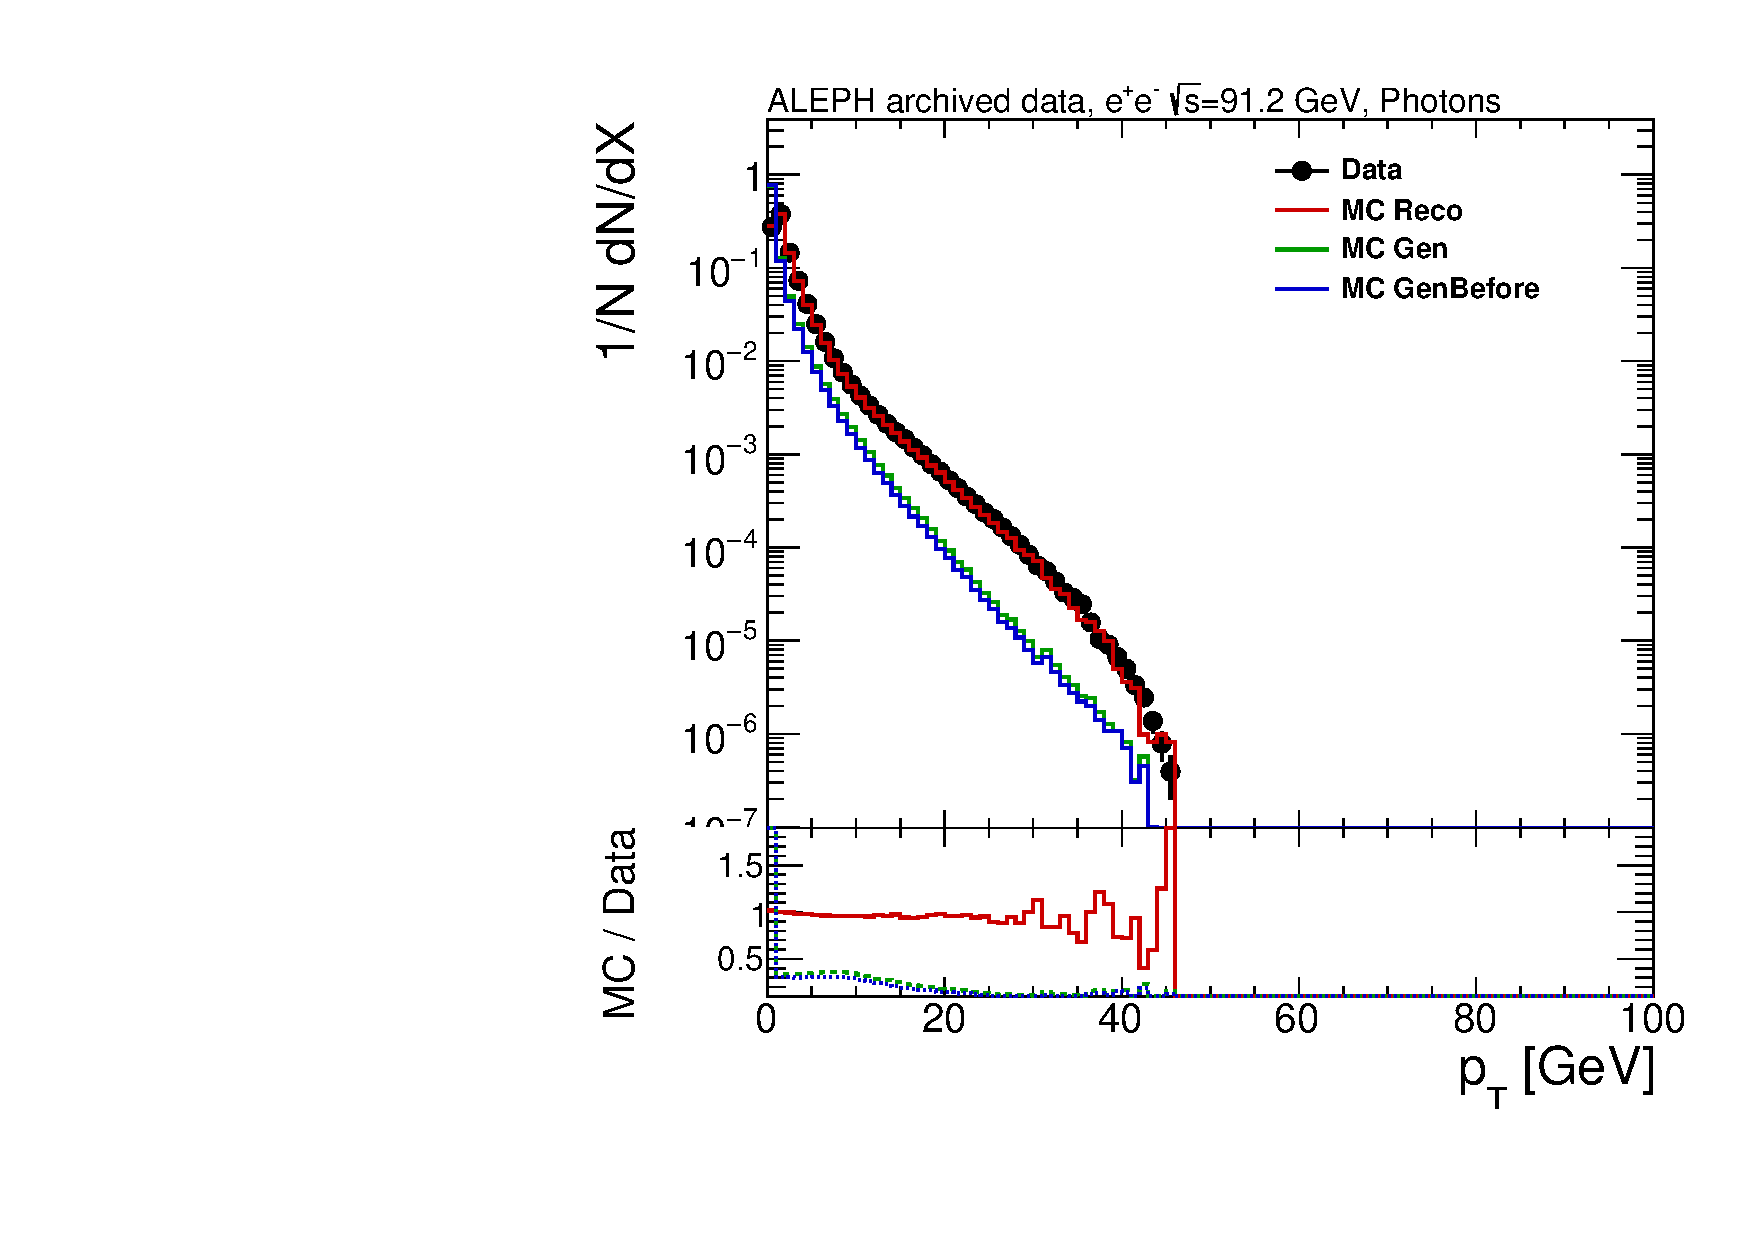
\includegraphics[width=0.242\textwidth]{figures/pwflag4_pt.pdf}
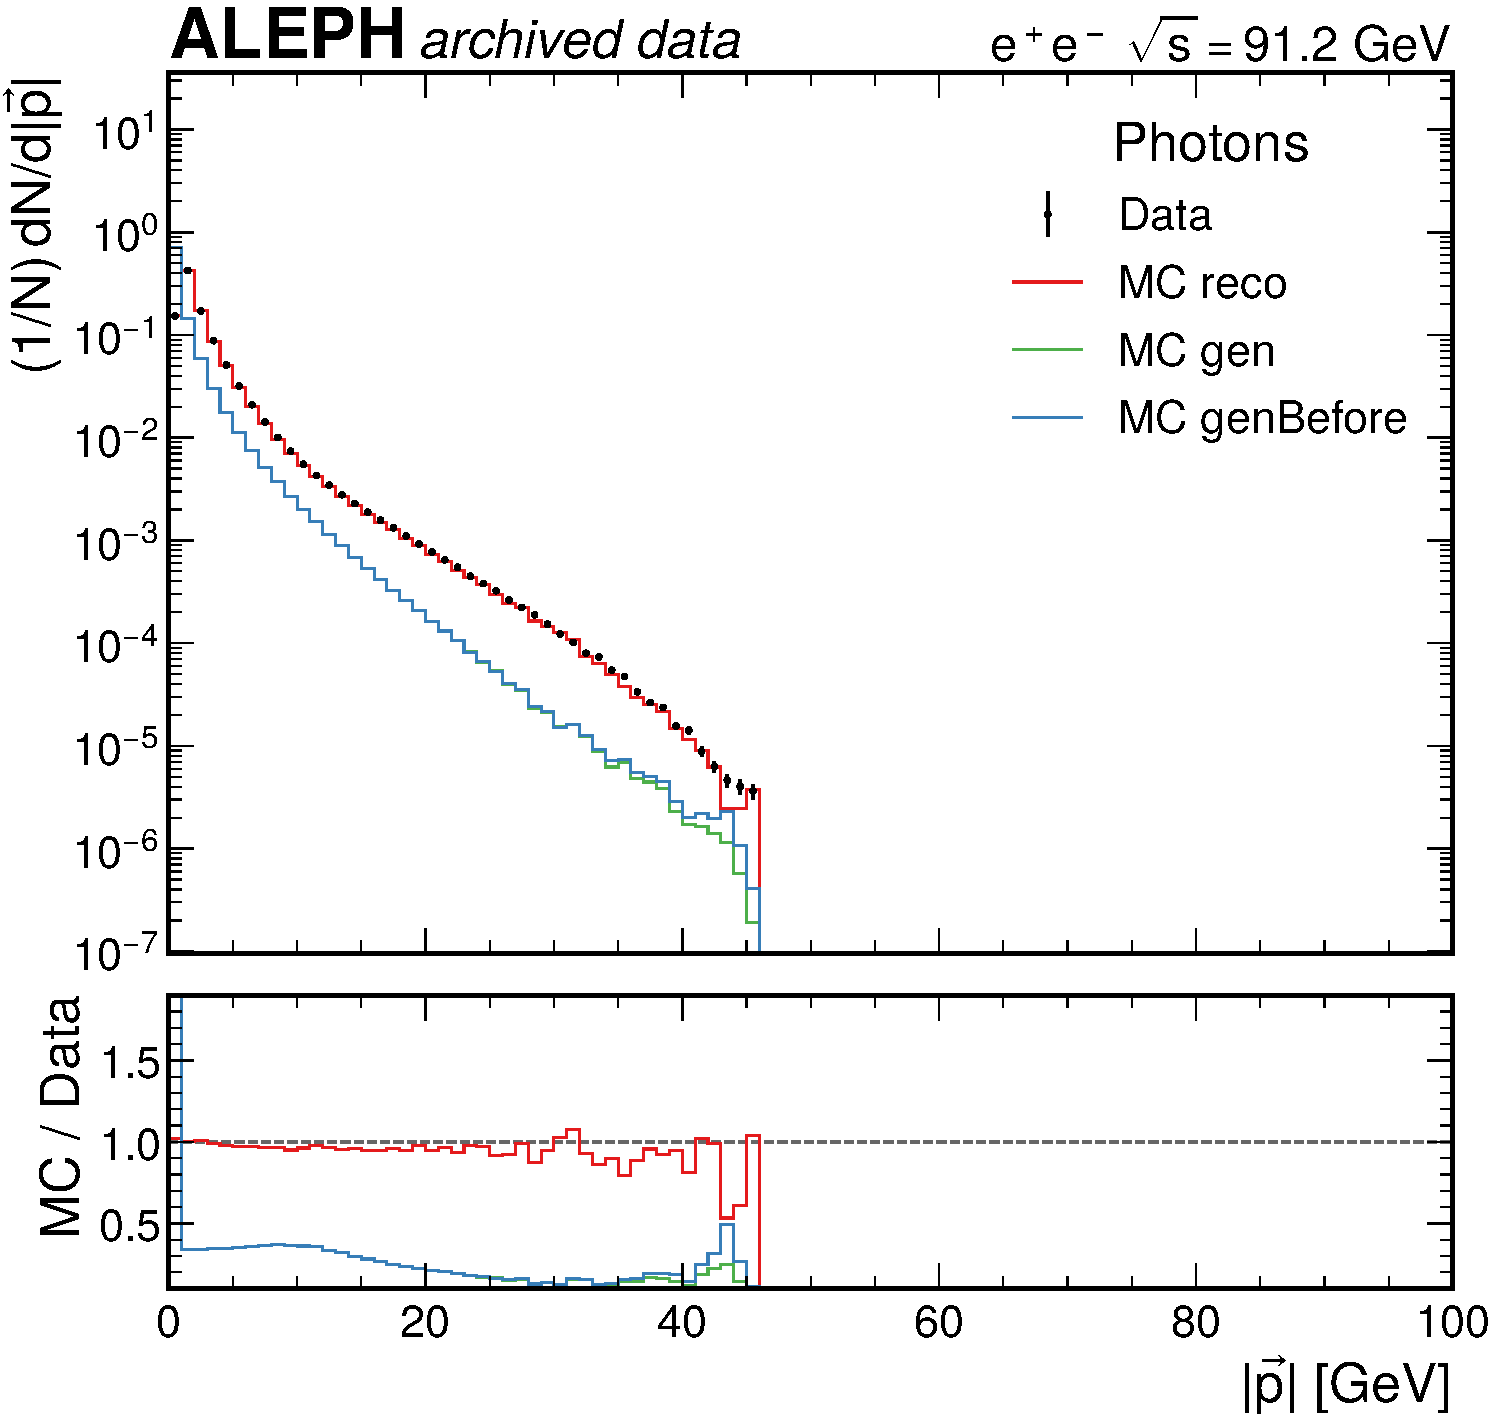
\includegraphics[width=0.495\textwidth]{figures/pwflag4_pmag.pdf}
% 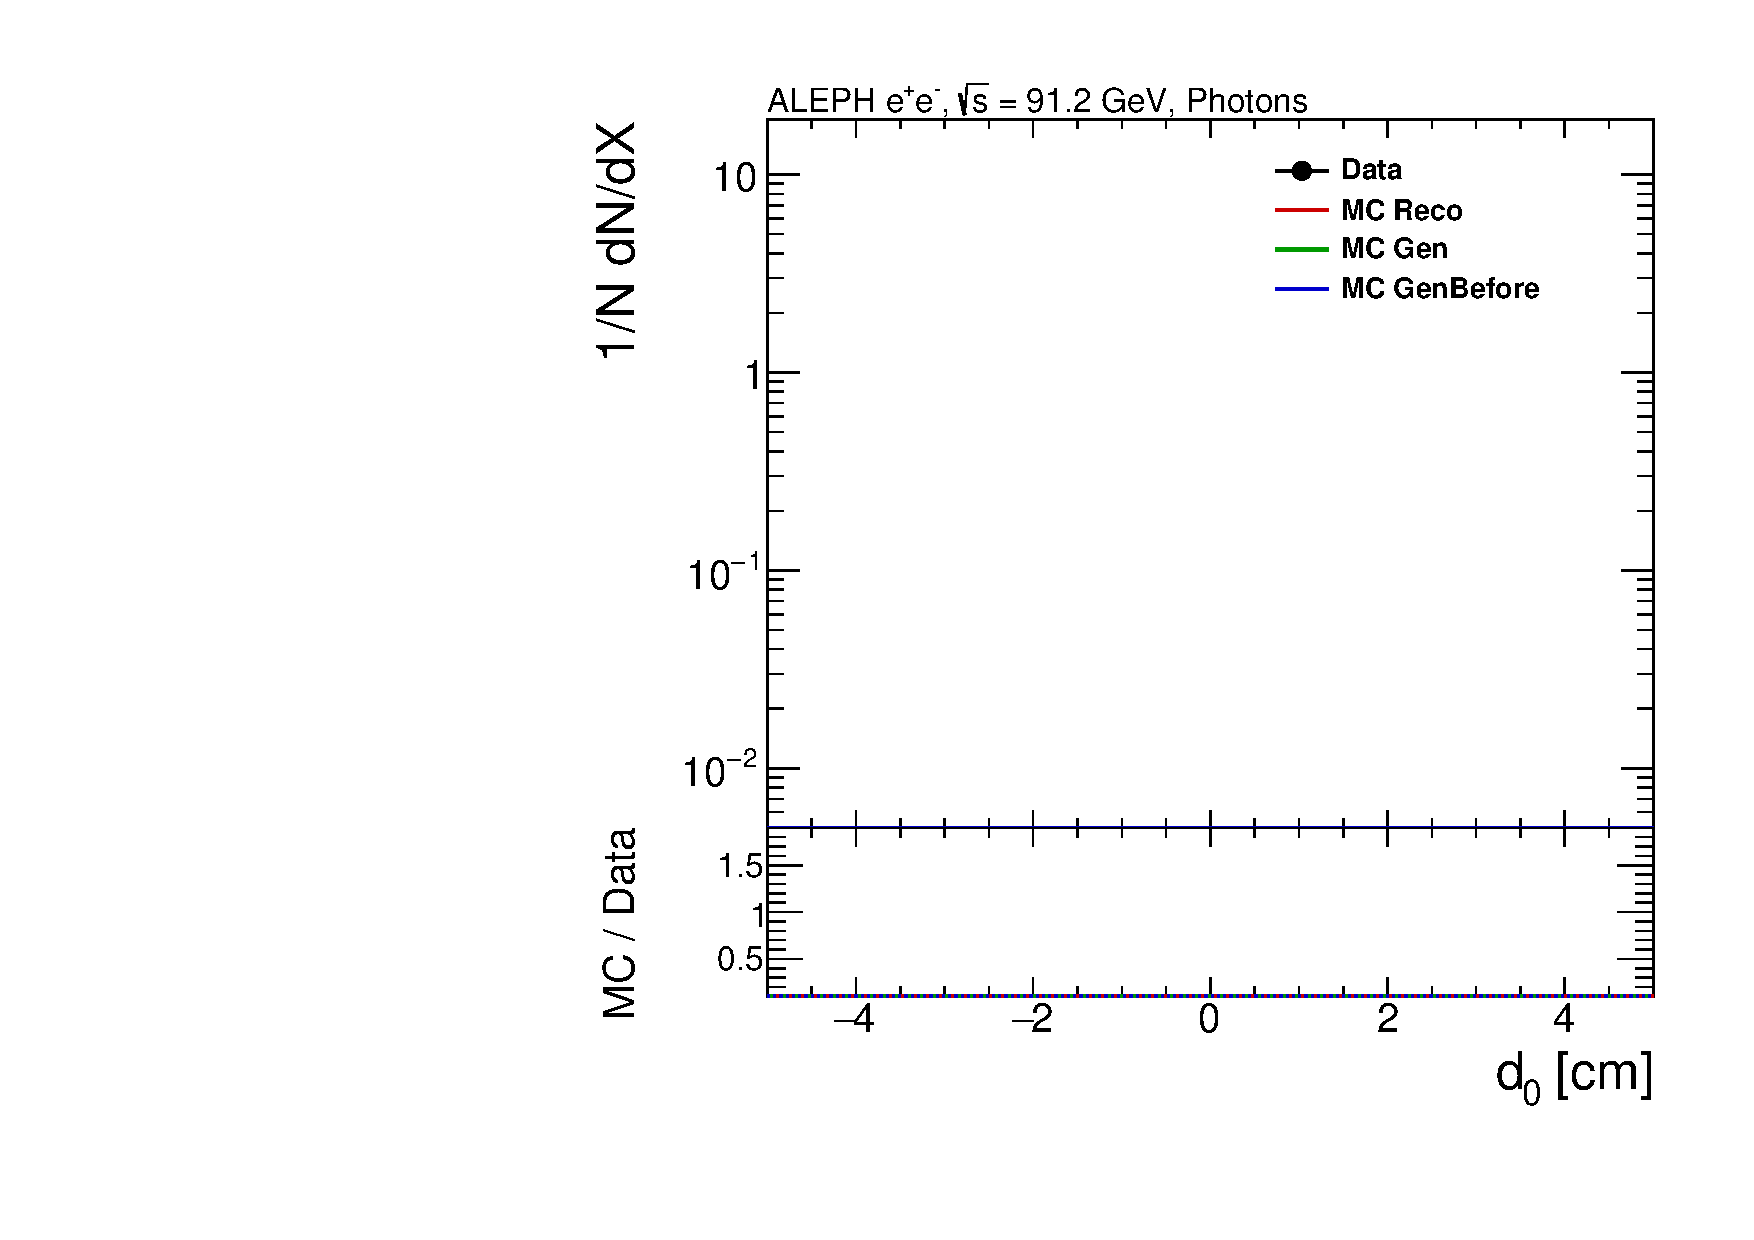
\includegraphics[width=0.242\textwidth]{figures/pwflag4_d0.pdf}
% 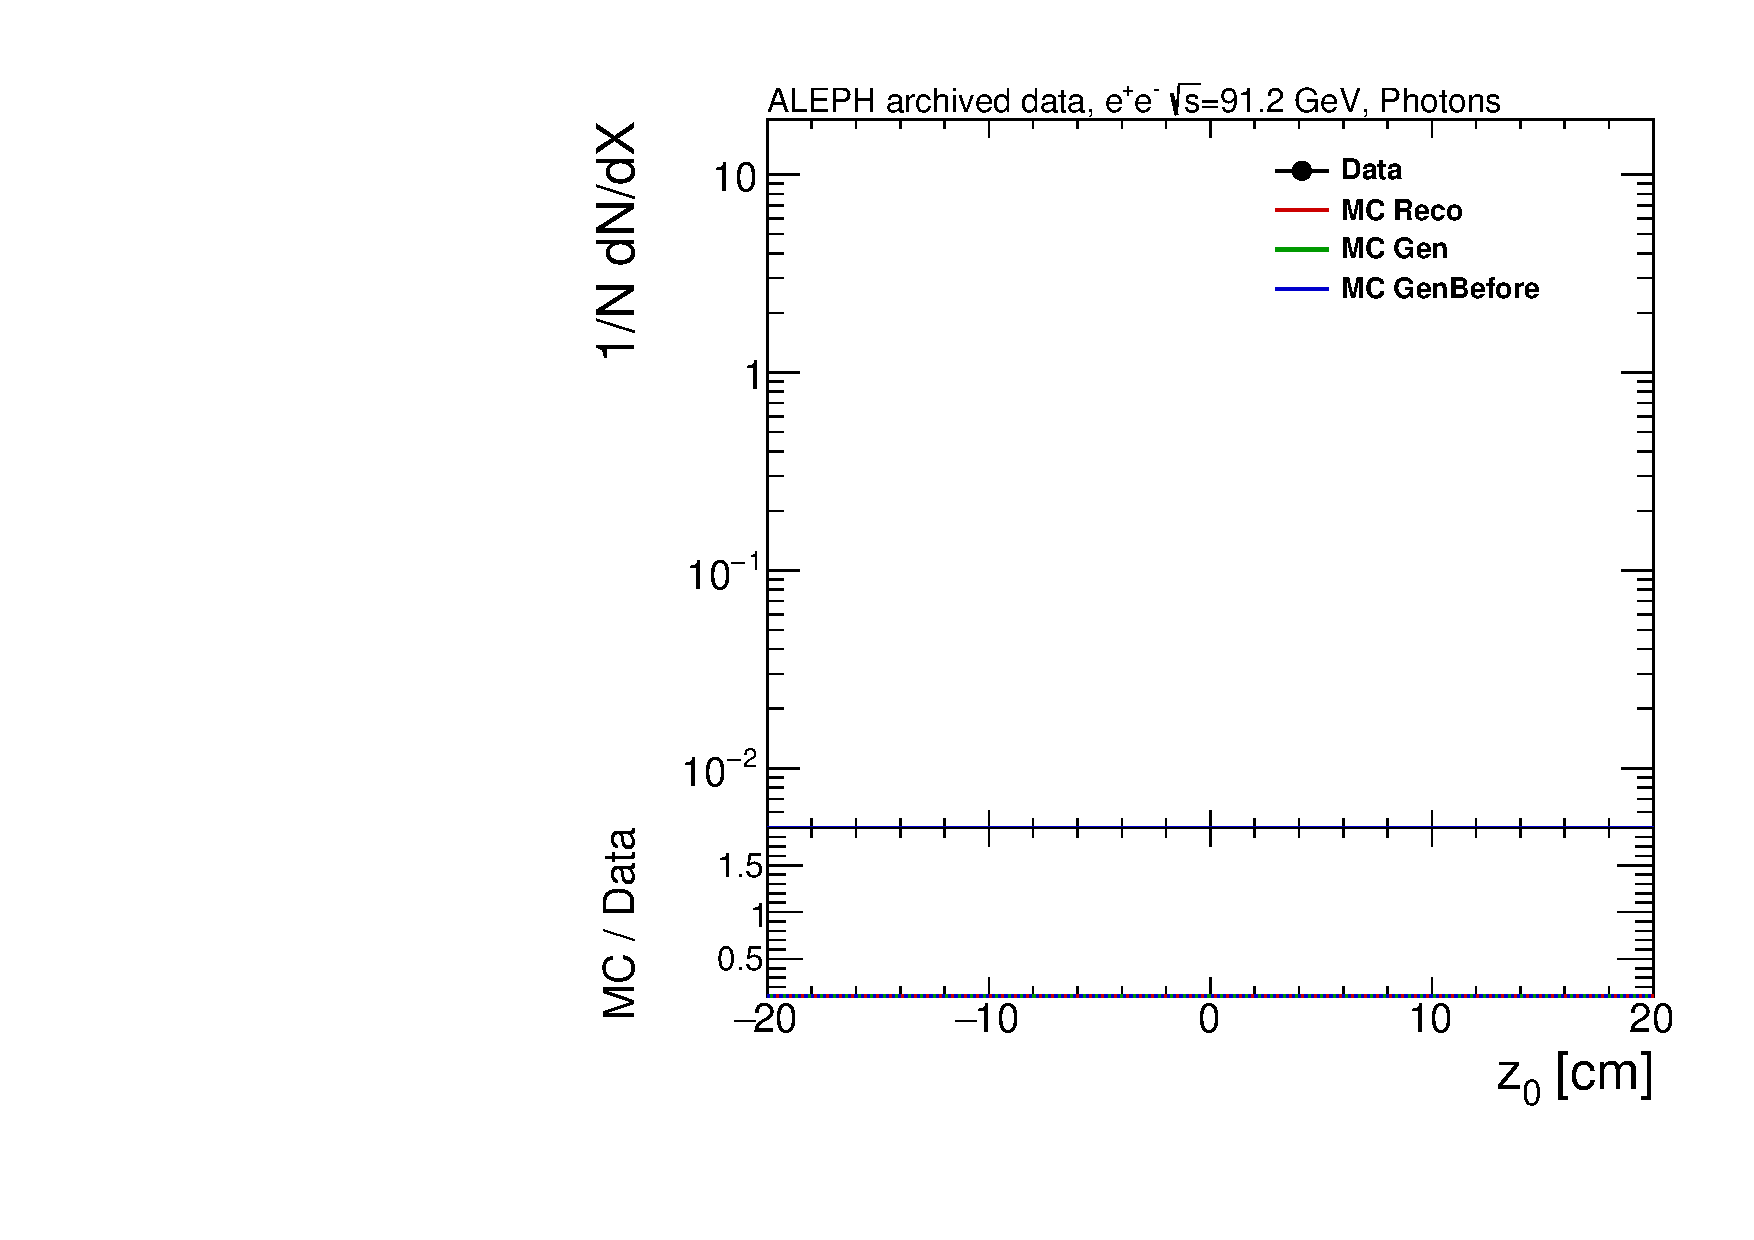
\includegraphics[width=0.242\textwidth]{figures/pwflag4_z0.pdf}
% 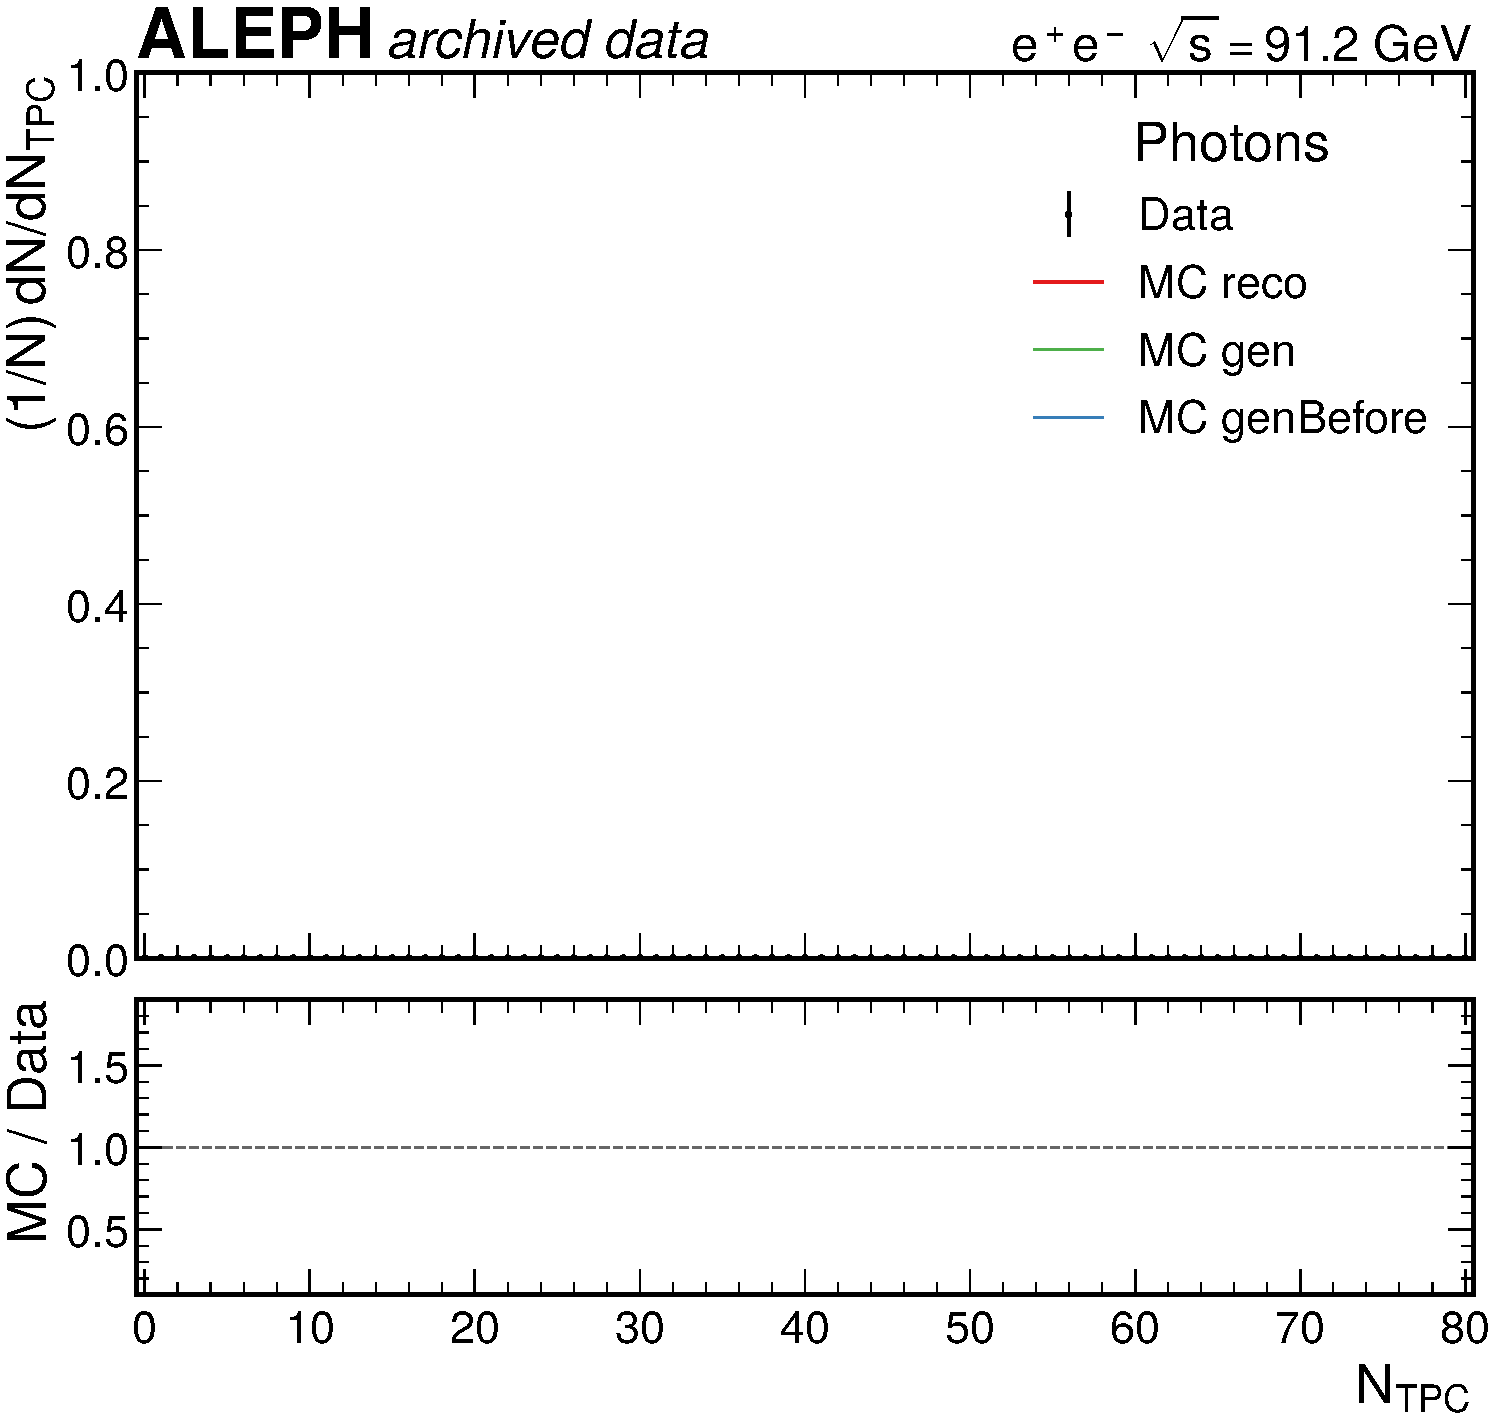
\includegraphics[width=0.242\textwidth]{figures/pwflag4_ntpc.pdf}
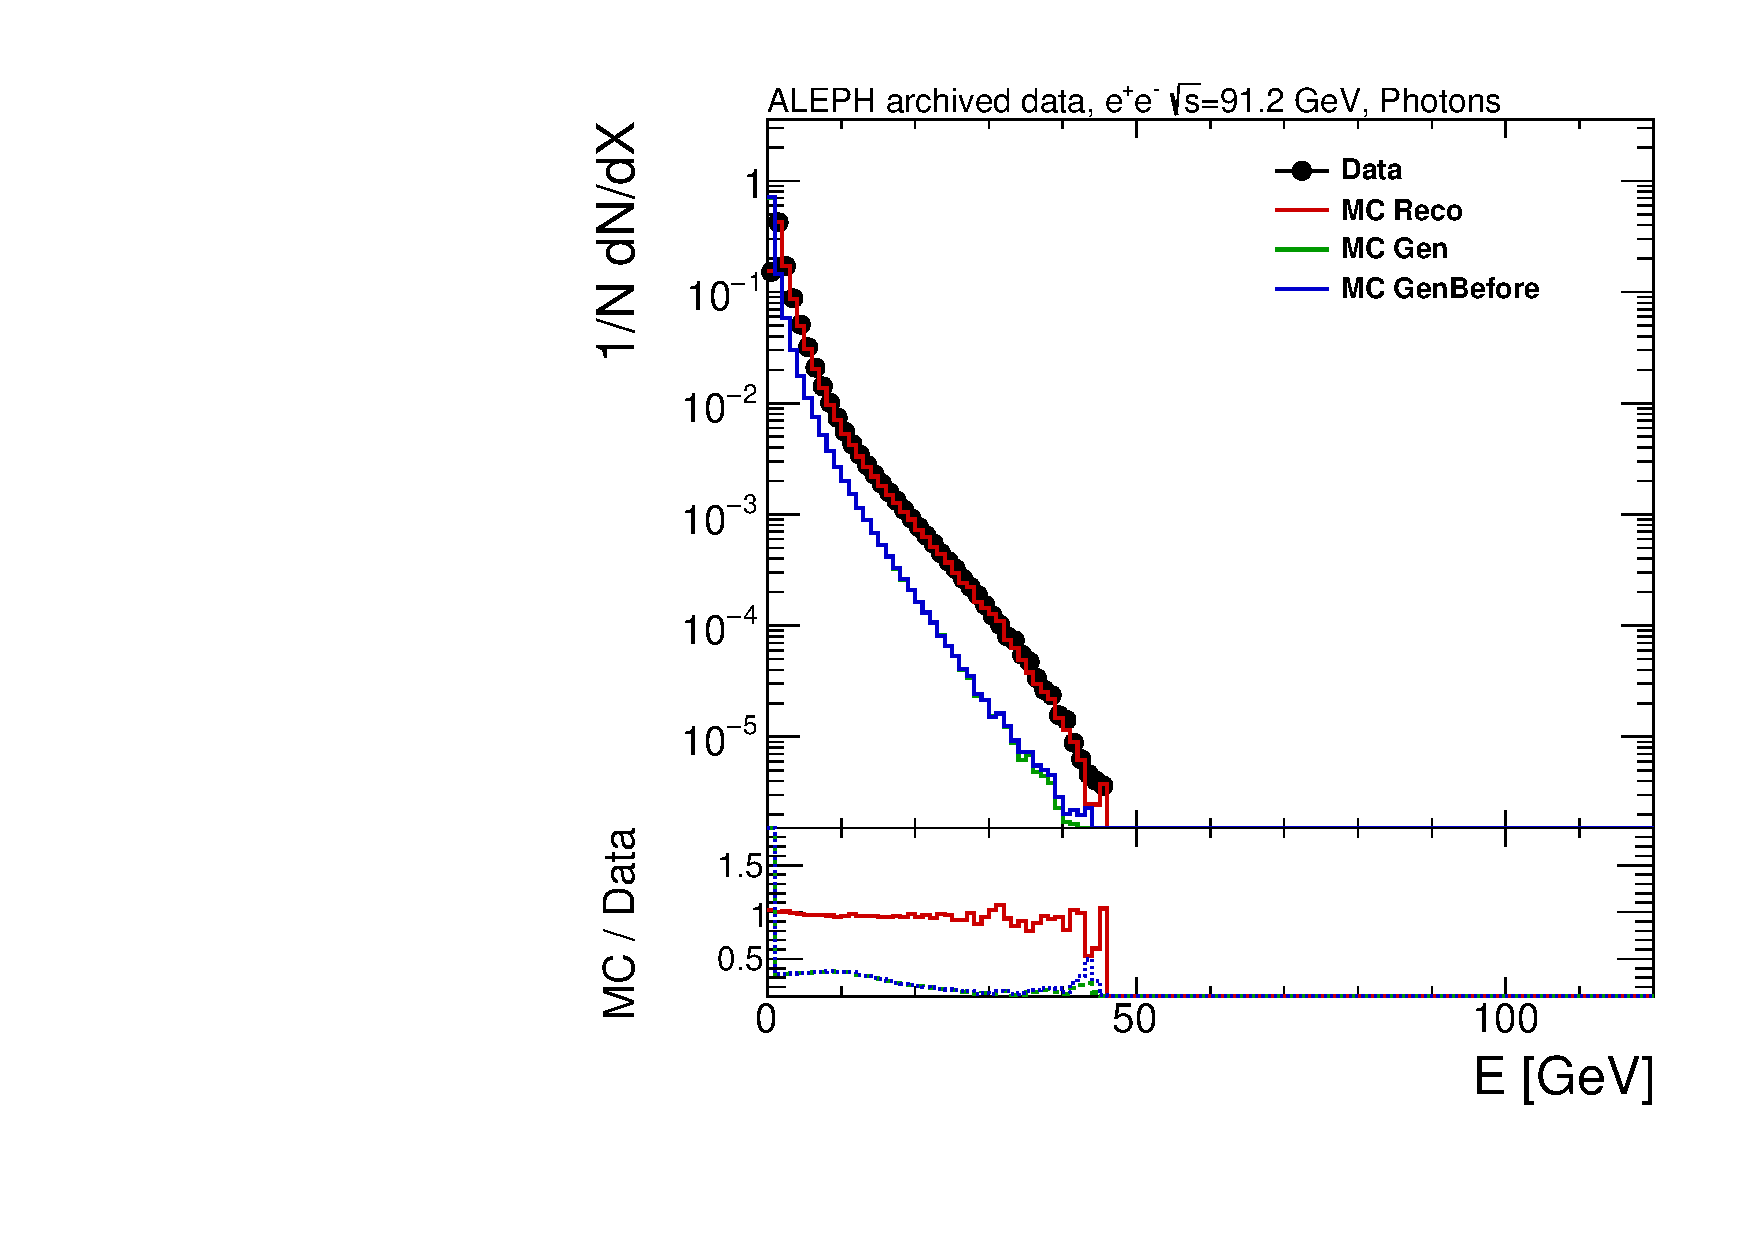
\includegraphics[width=0.495\textwidth]{figures/pwflag4_energy.pdf}
% 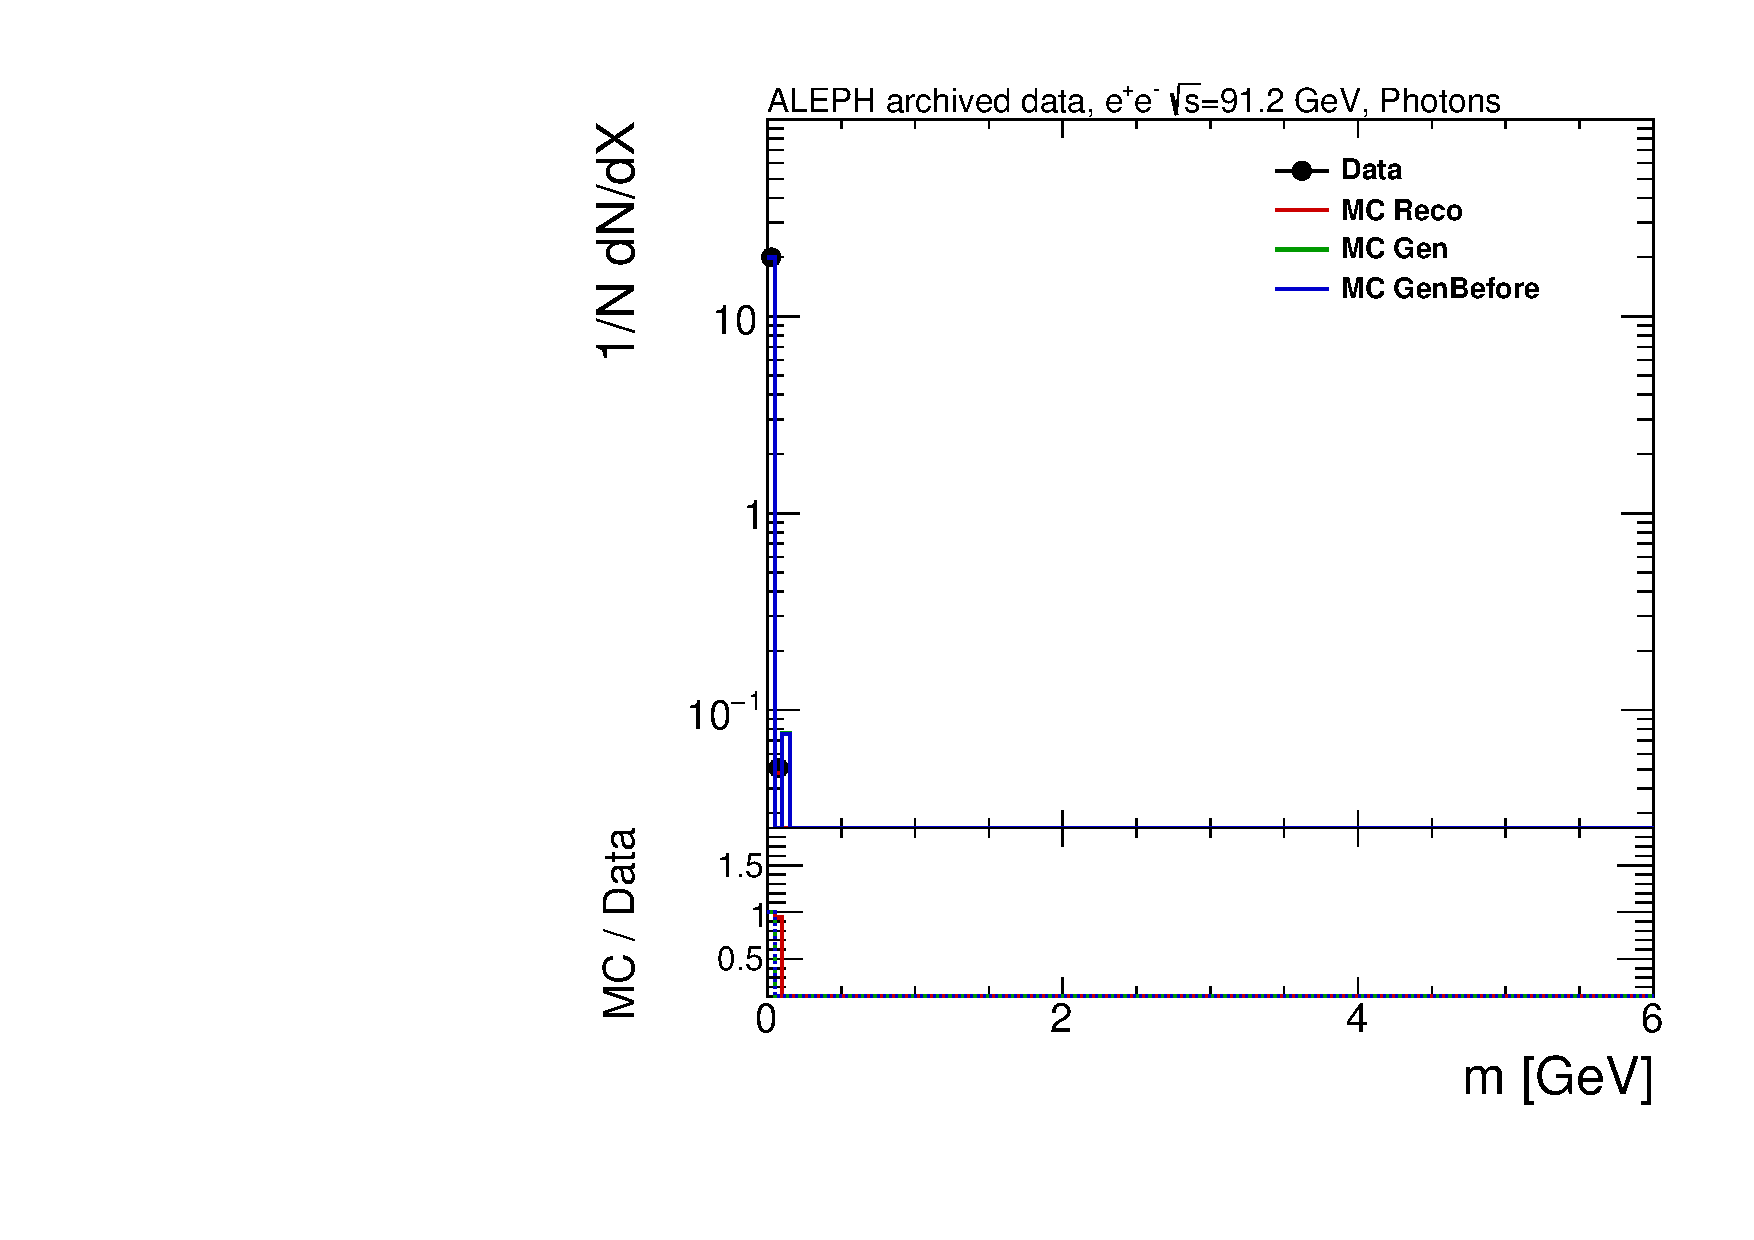
\includegraphics[width=0.495\textwidth]{figures/pwflag4_mass.pdf}
\caption{Complete \texttt{pwflag}=4 kinematic set.}
\label{fig:pwflag4_full}
\end{figure}

\FloatBarrier

\begin{figure}[t!]
\centering
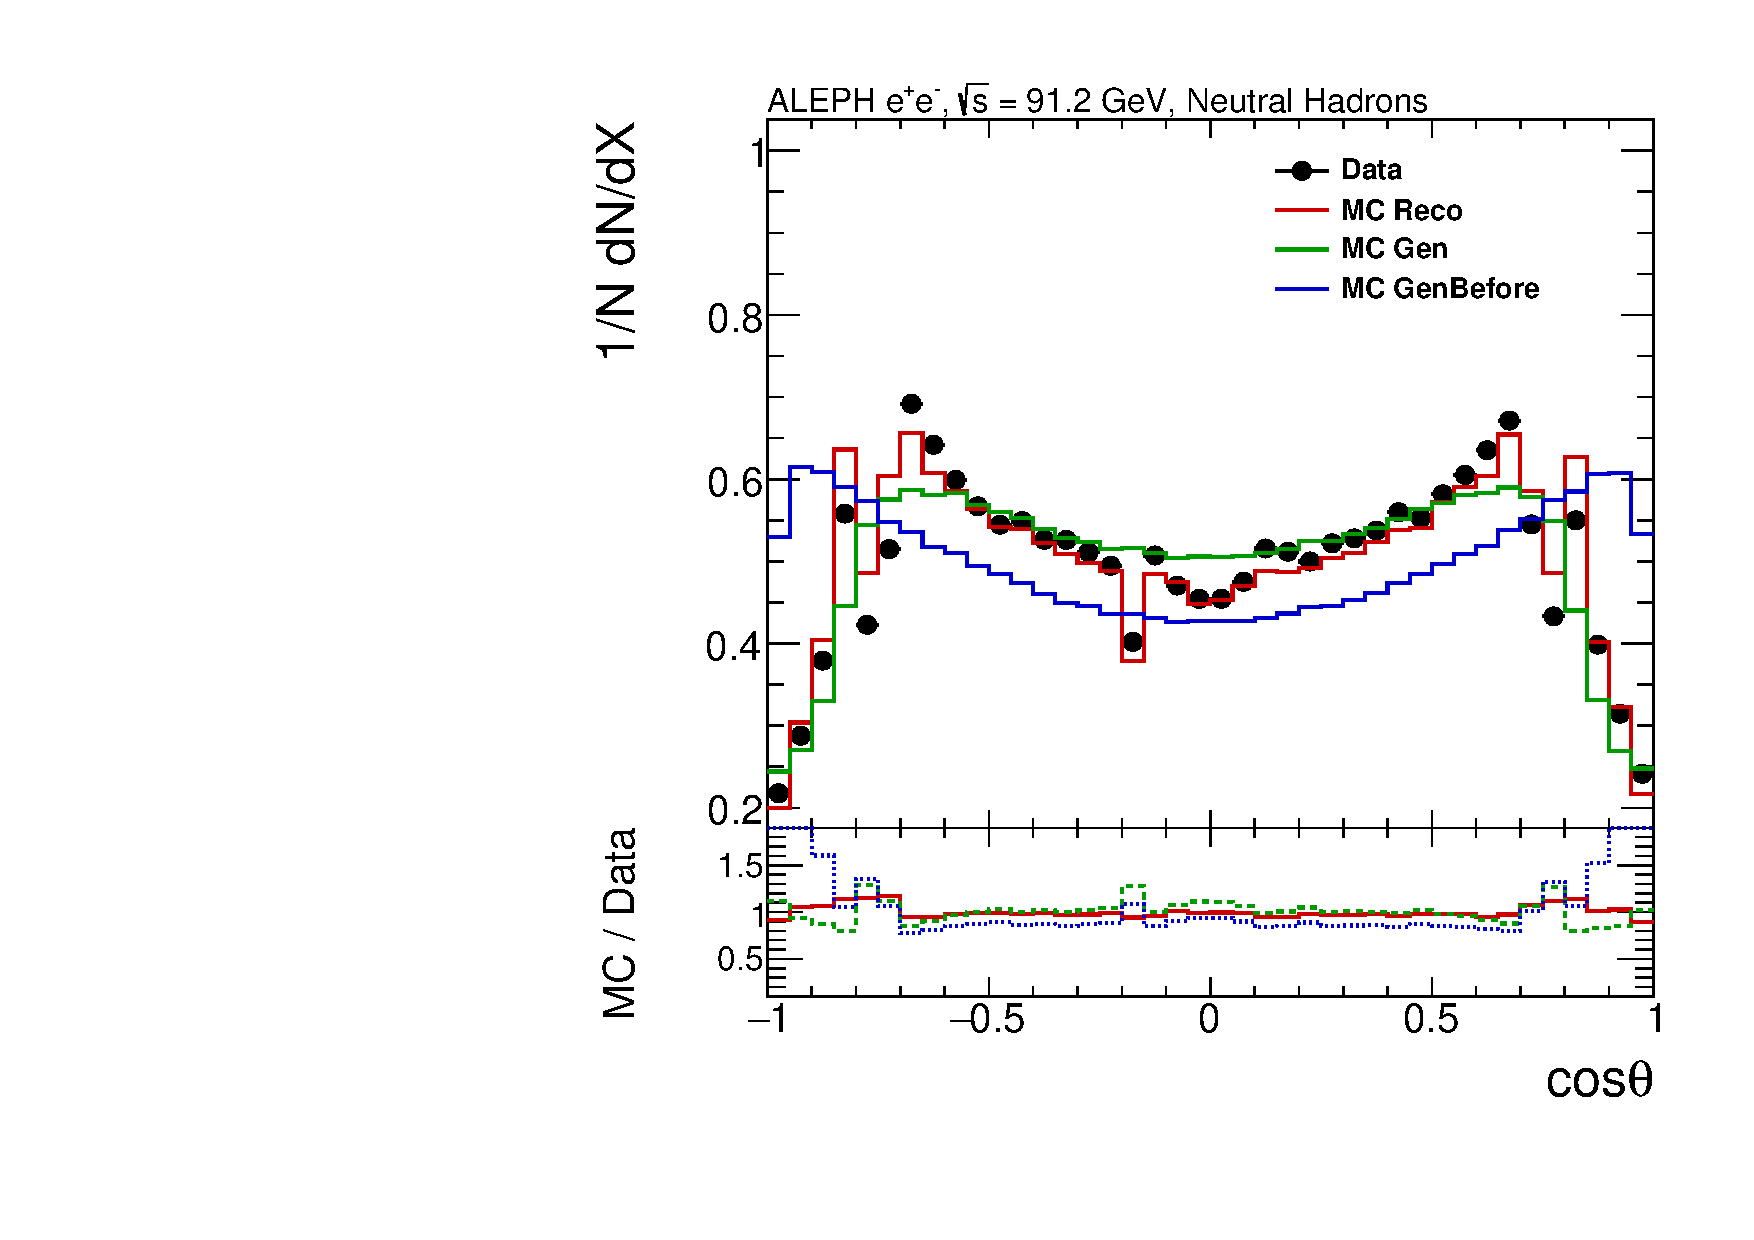
\includegraphics[width=0.495\textwidth]{figures/pwflag5_cosTheta.pdf}
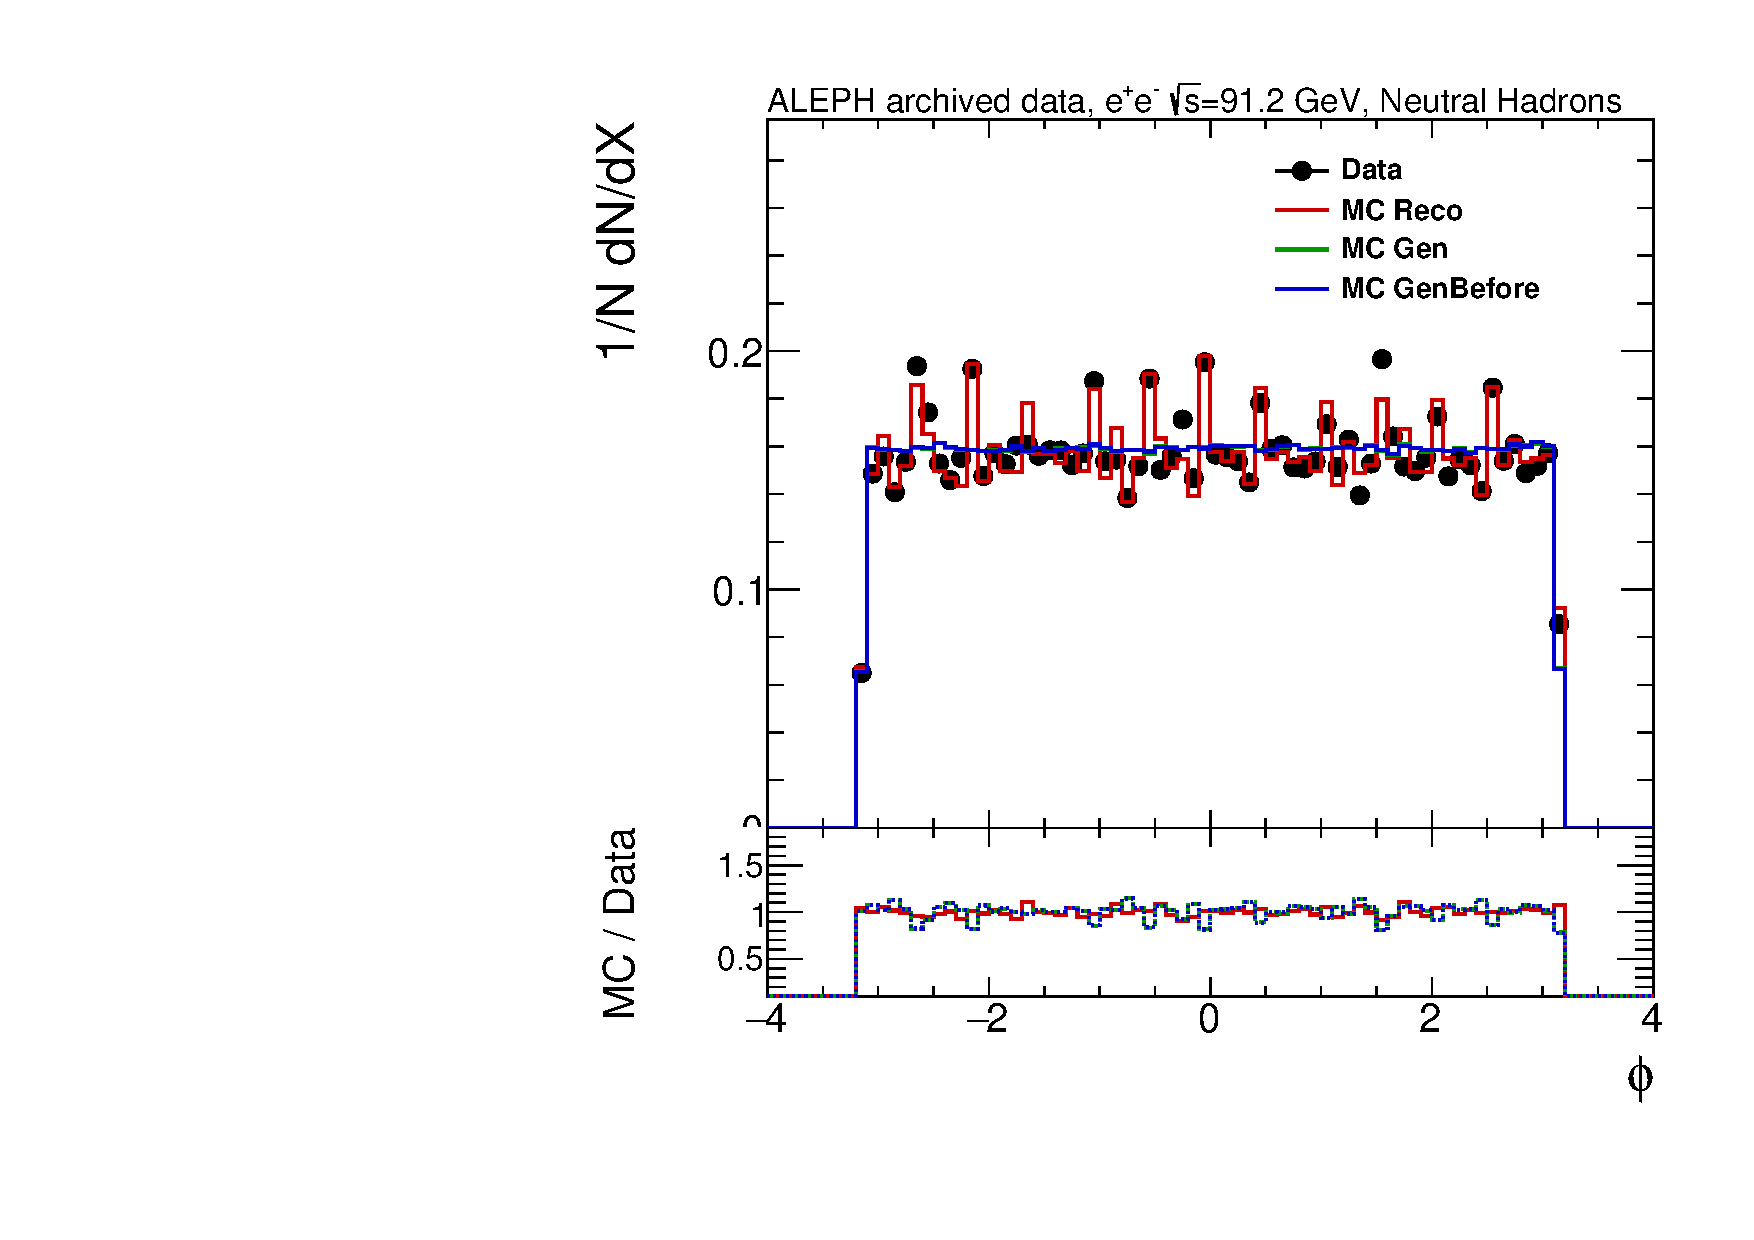
\includegraphics[width=0.495\textwidth]{figures/pwflag5_phi.pdf}
% 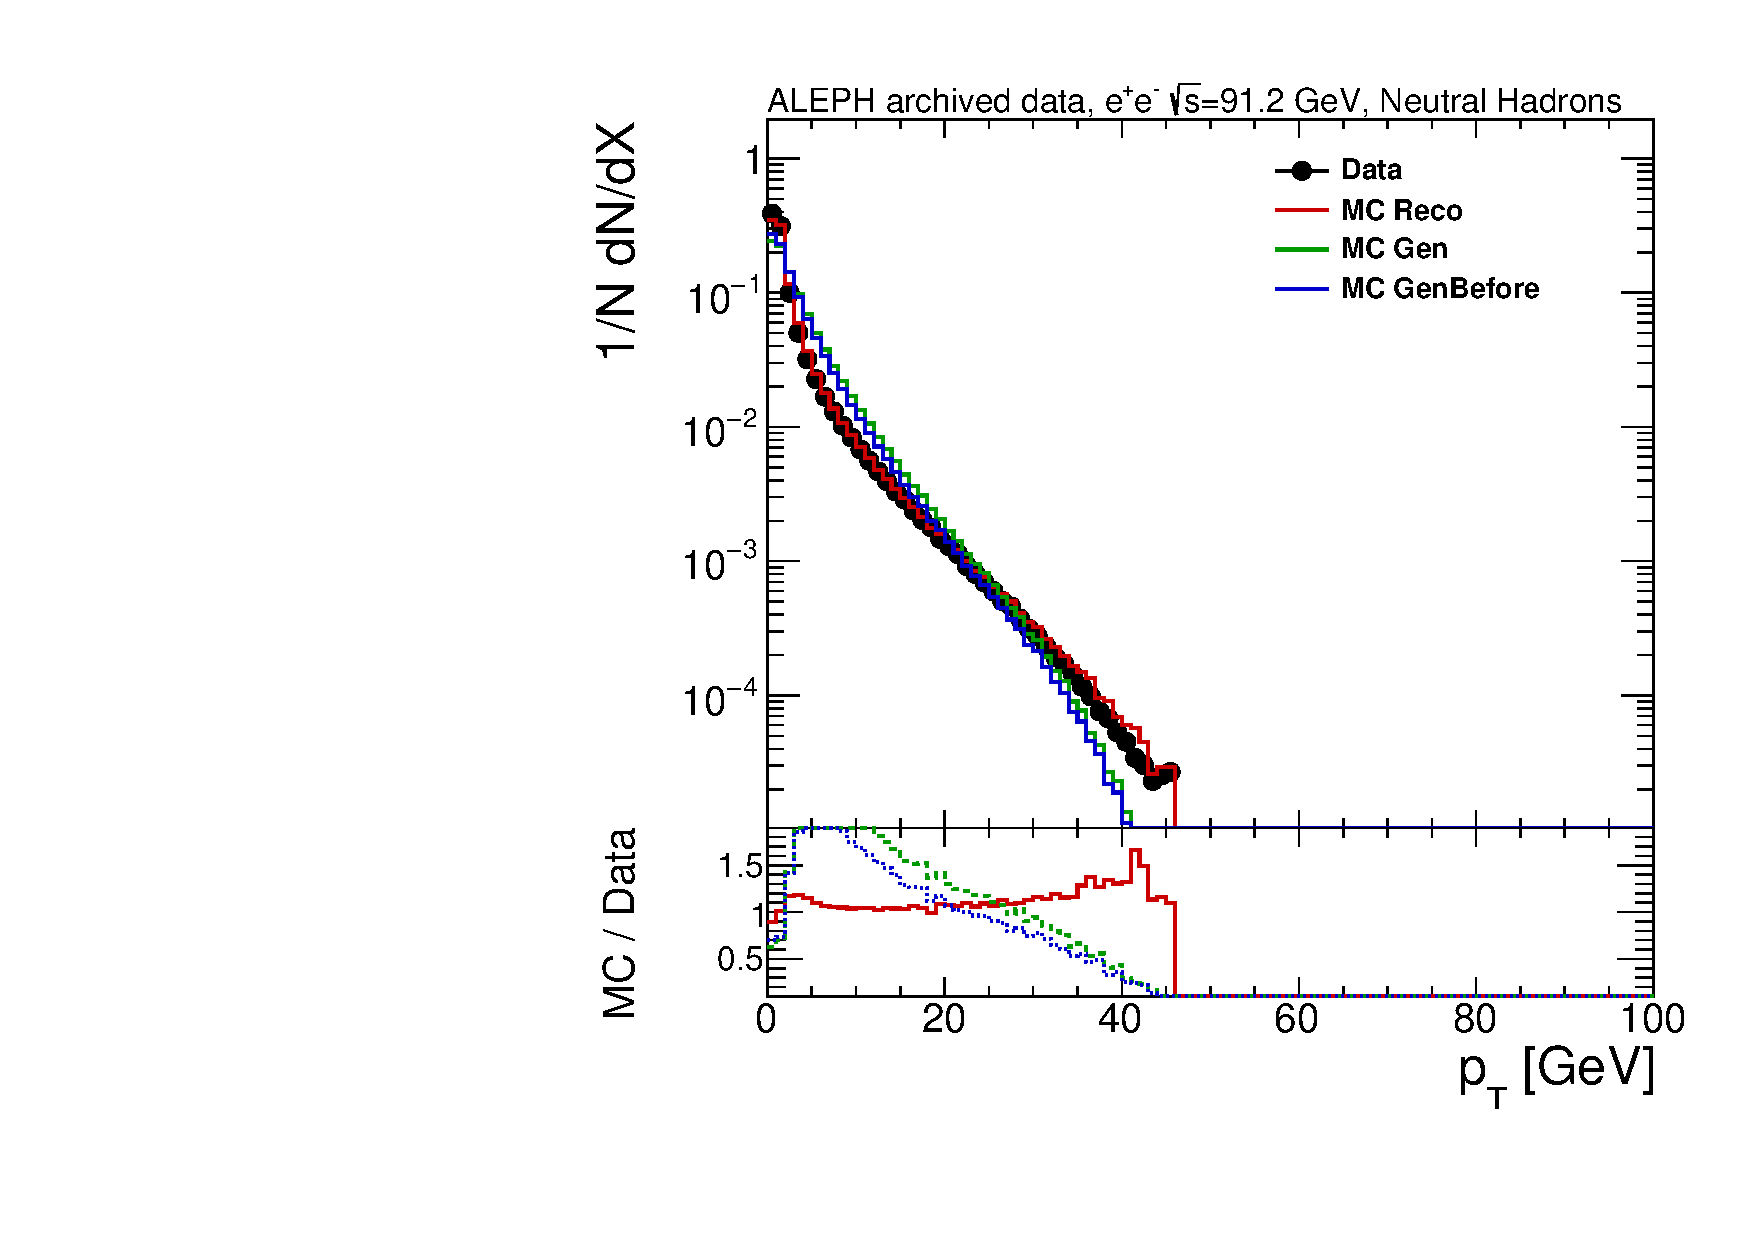
\includegraphics[width=0.242\textwidth]{figures/pwflag5_pt.pdf}
% 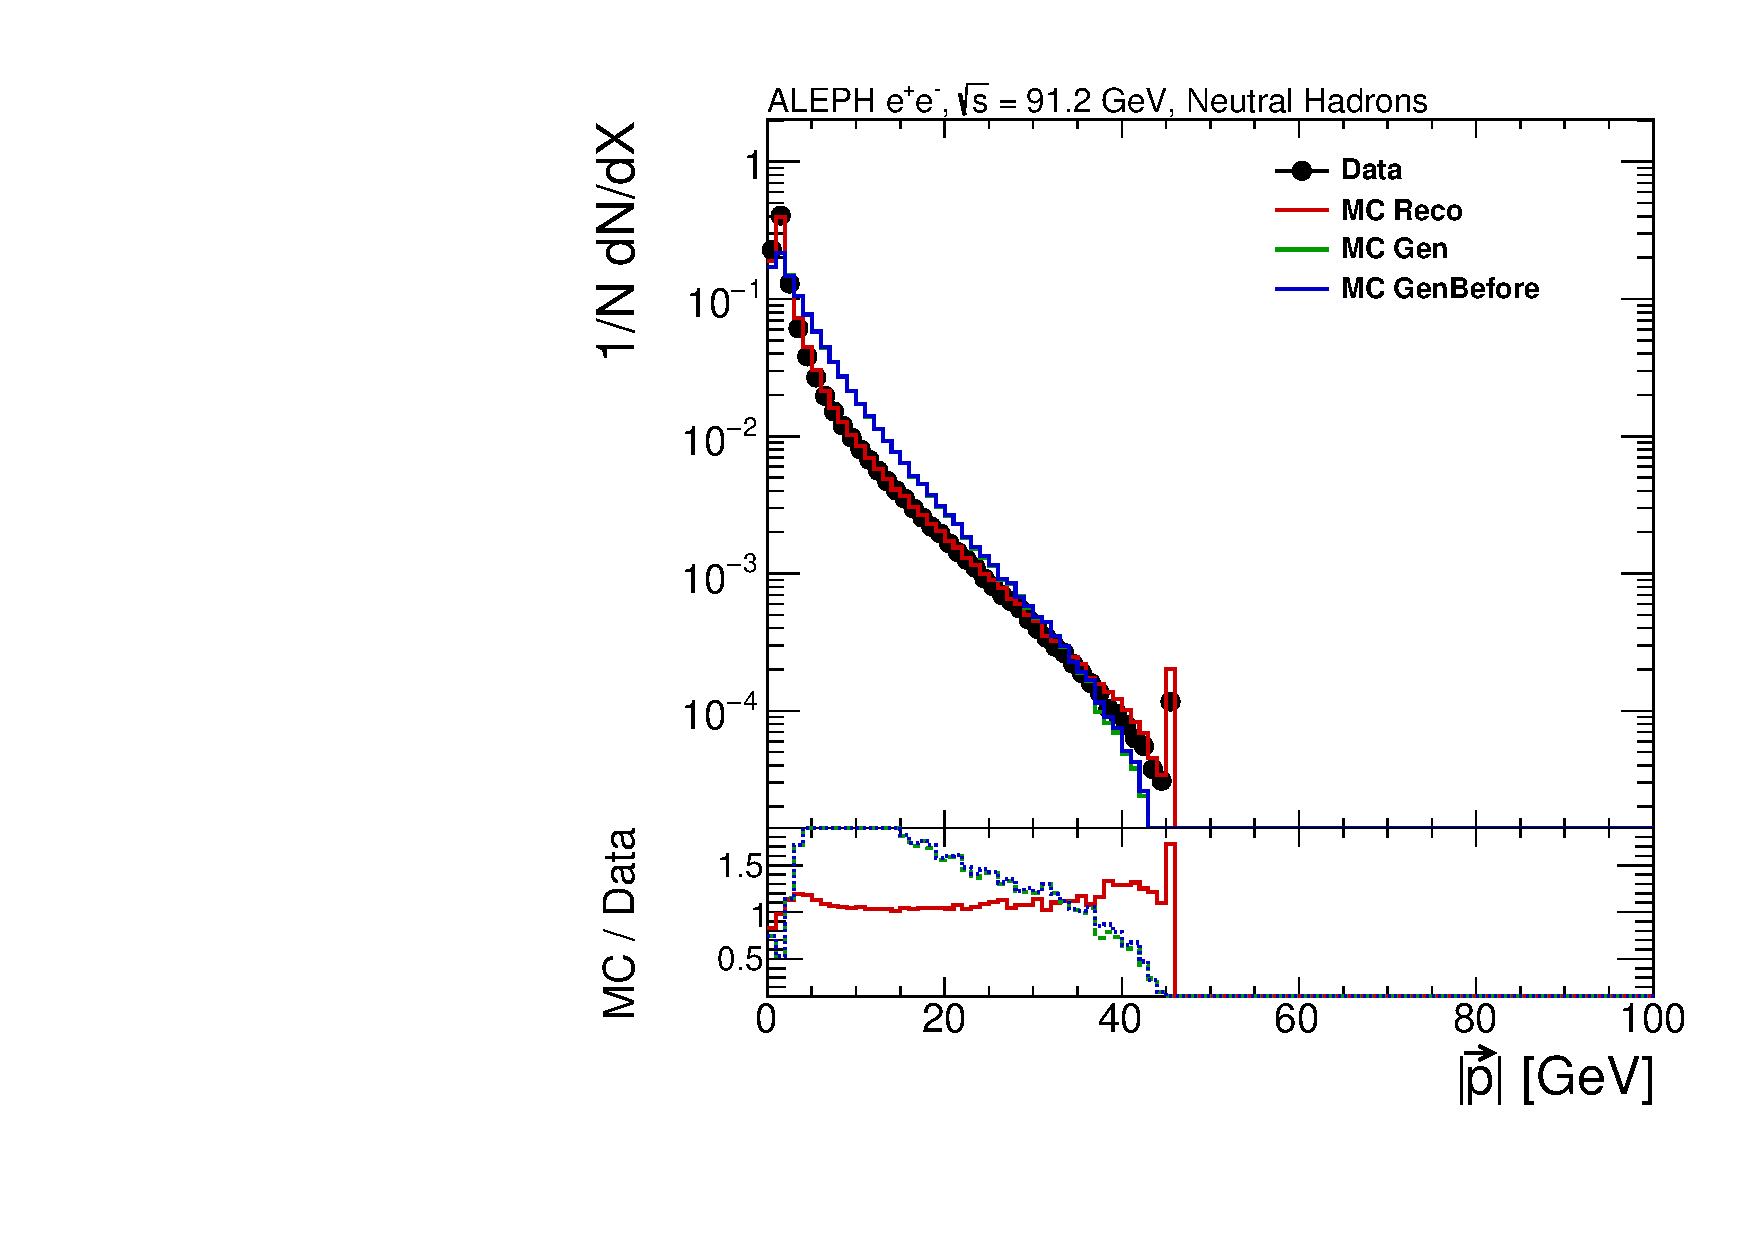
\includegraphics[width=0.242\textwidth]{figures/pwflag5_pmag.pdf}
% 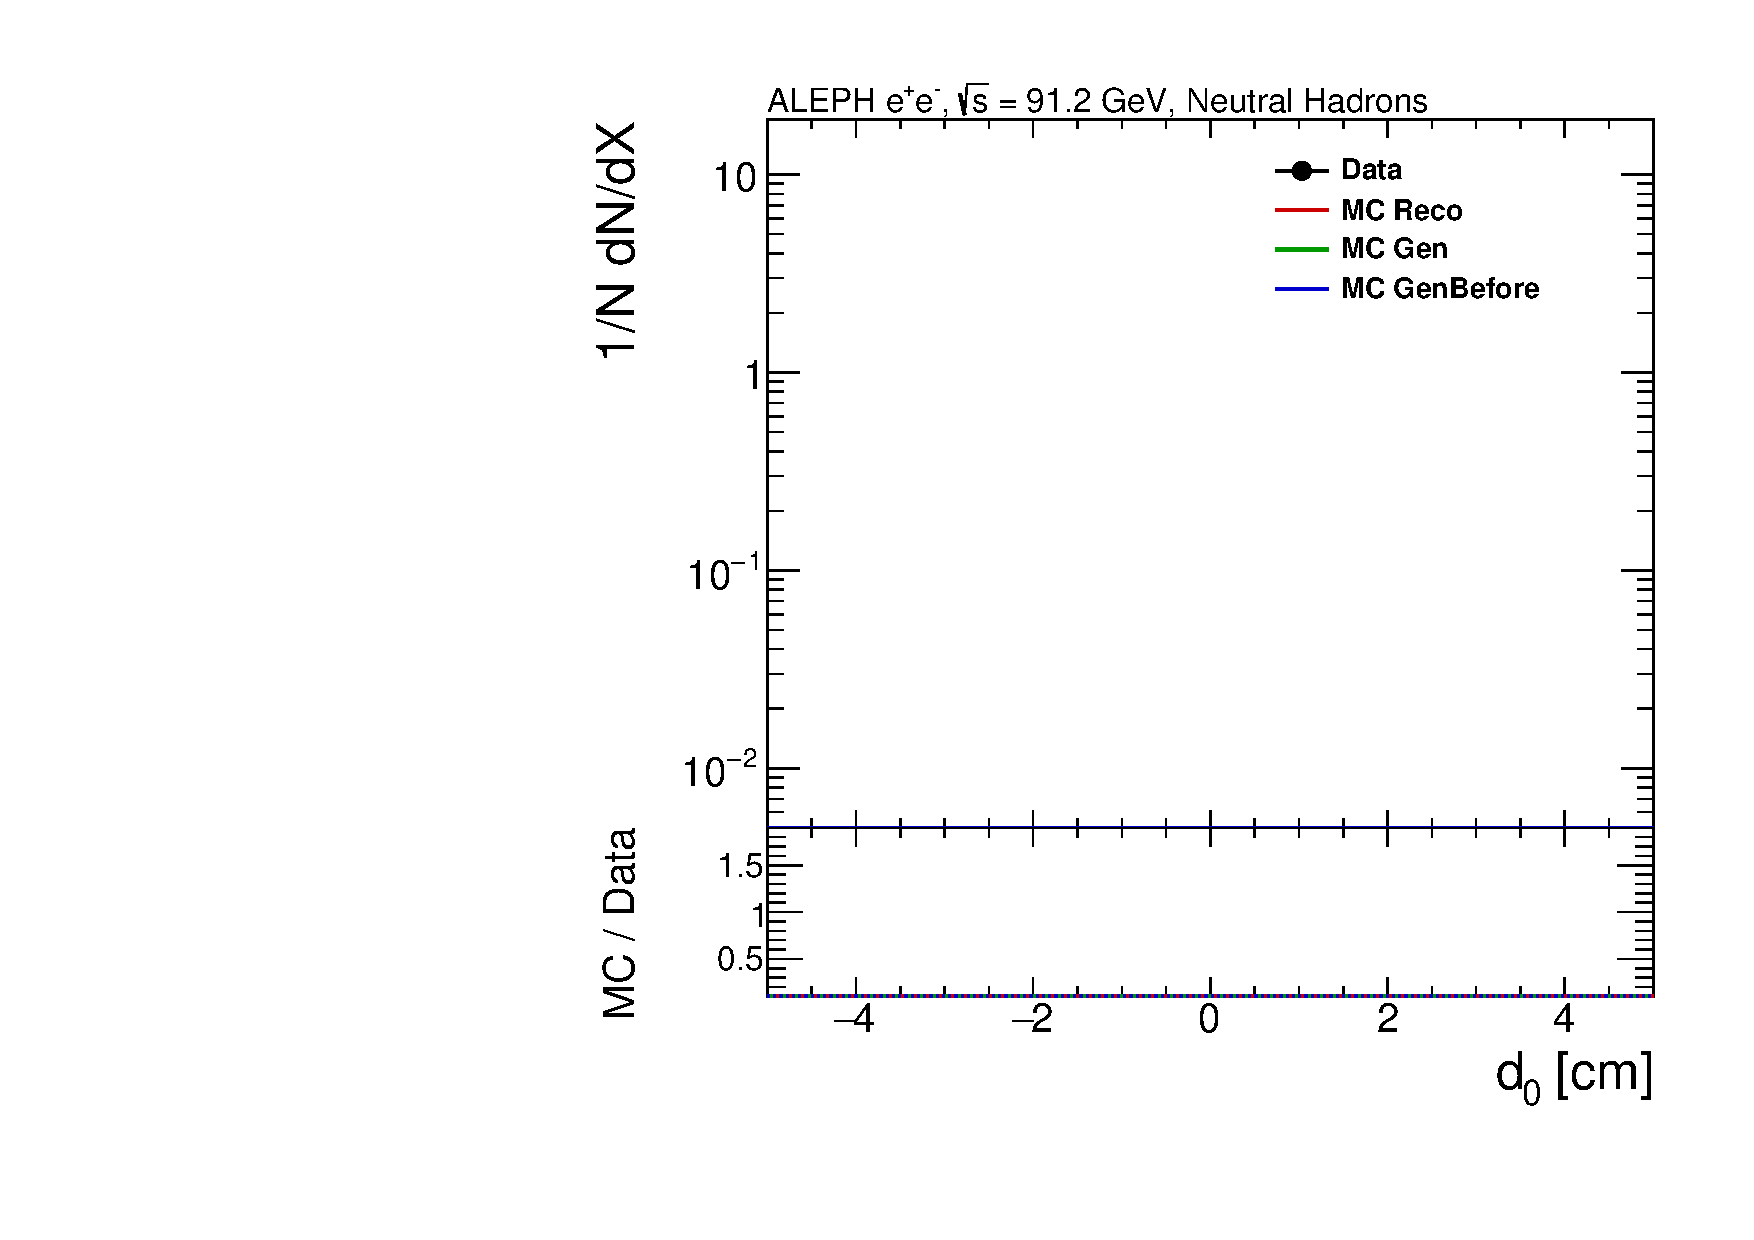
\includegraphics[width=0.242\textwidth]{figures/pwflag5_d0.pdf}
% 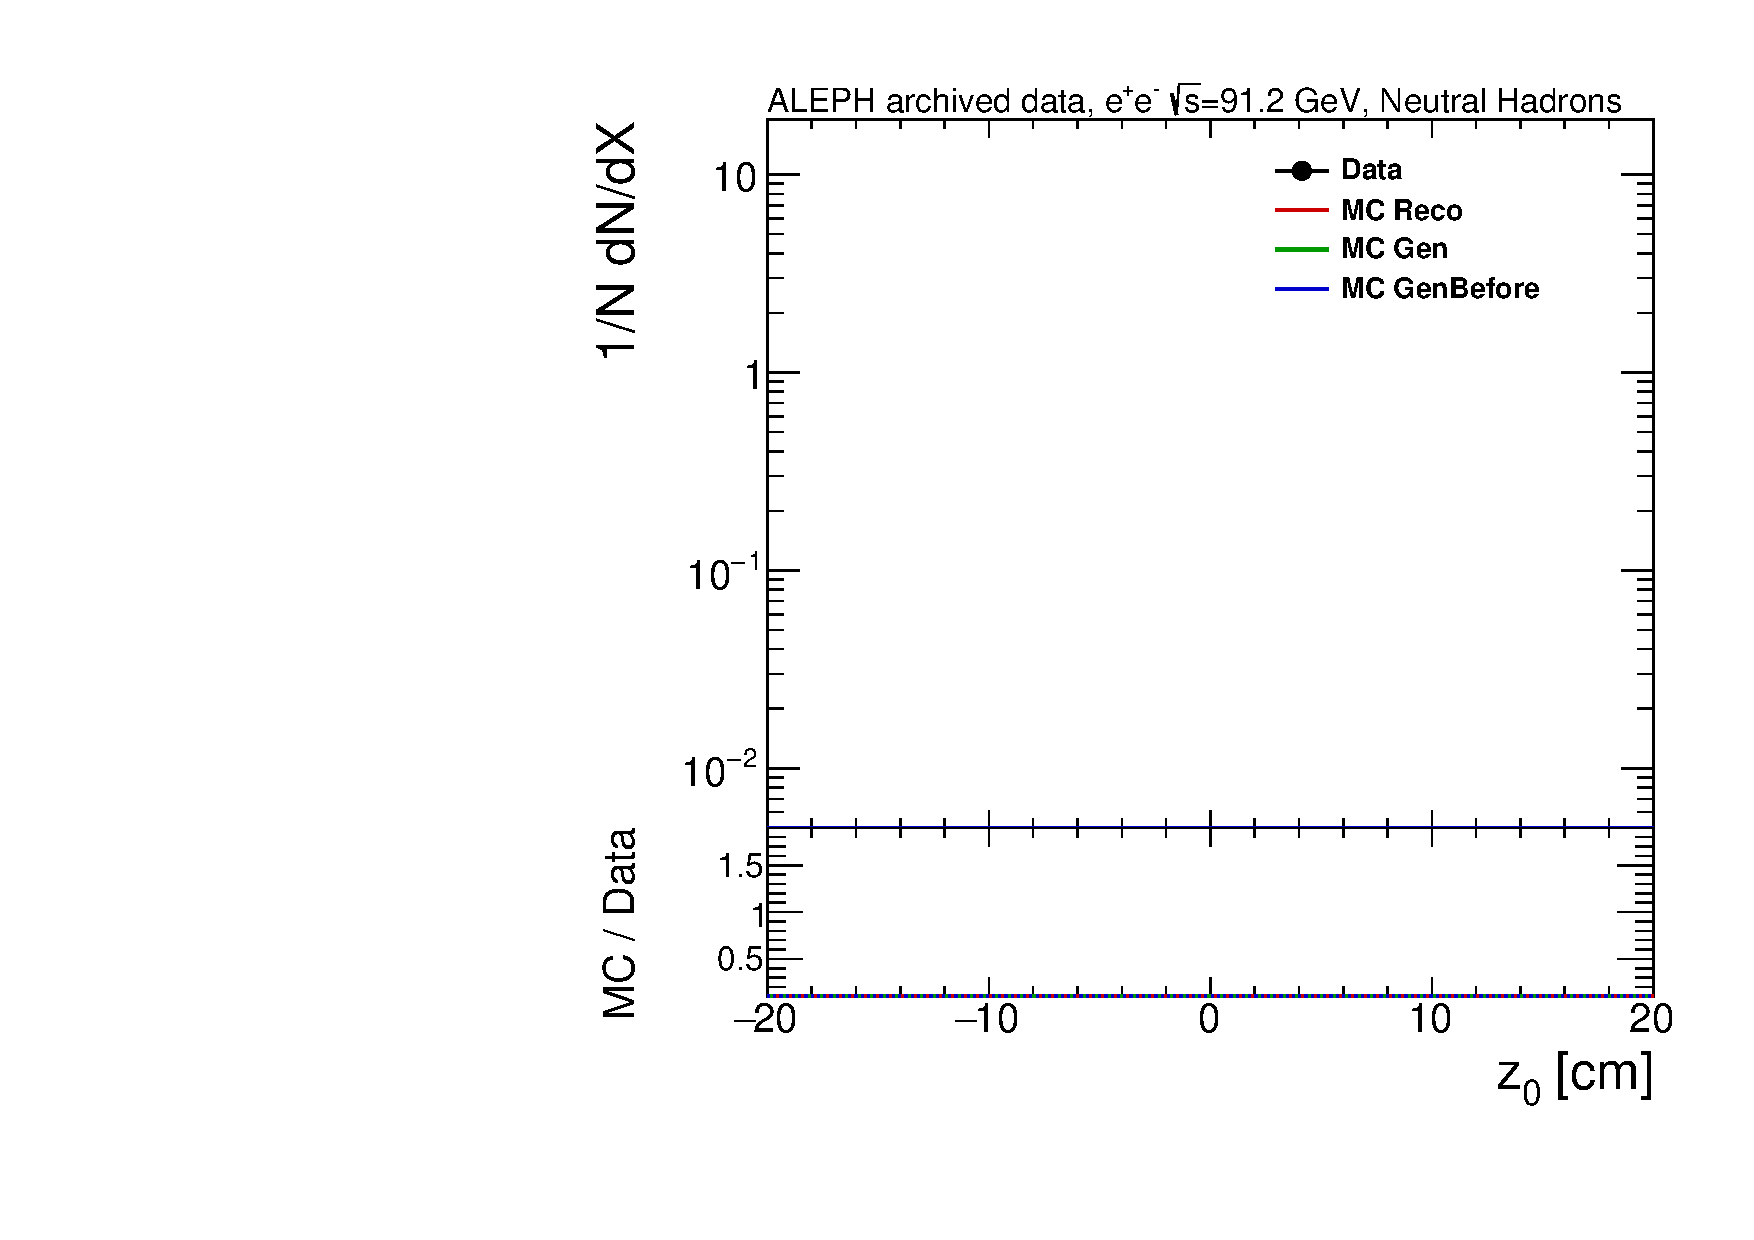
\includegraphics[width=0.242\textwidth]{figures/pwflag5_z0.pdf}
% 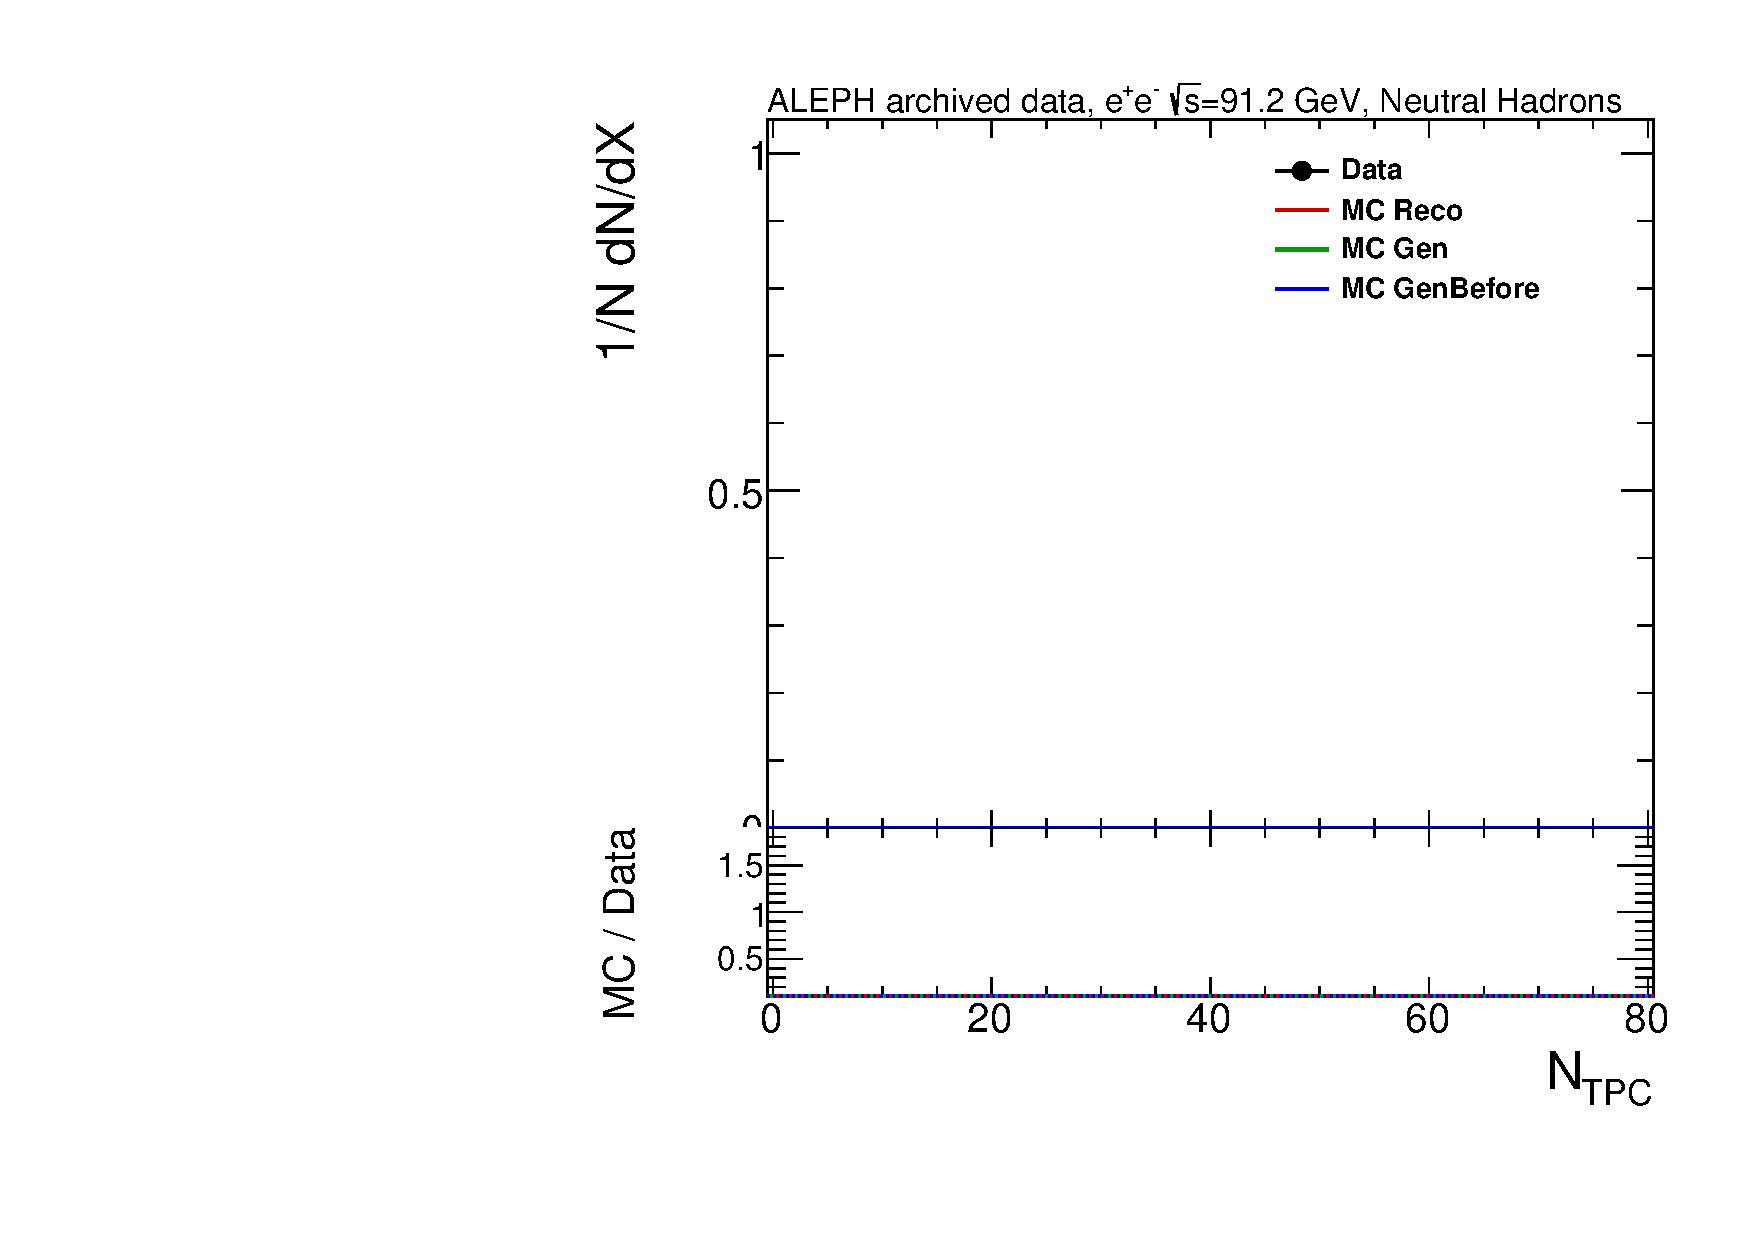
\includegraphics[width=0.242\textwidth]{figures/pwflag5_ntpc.pdf}
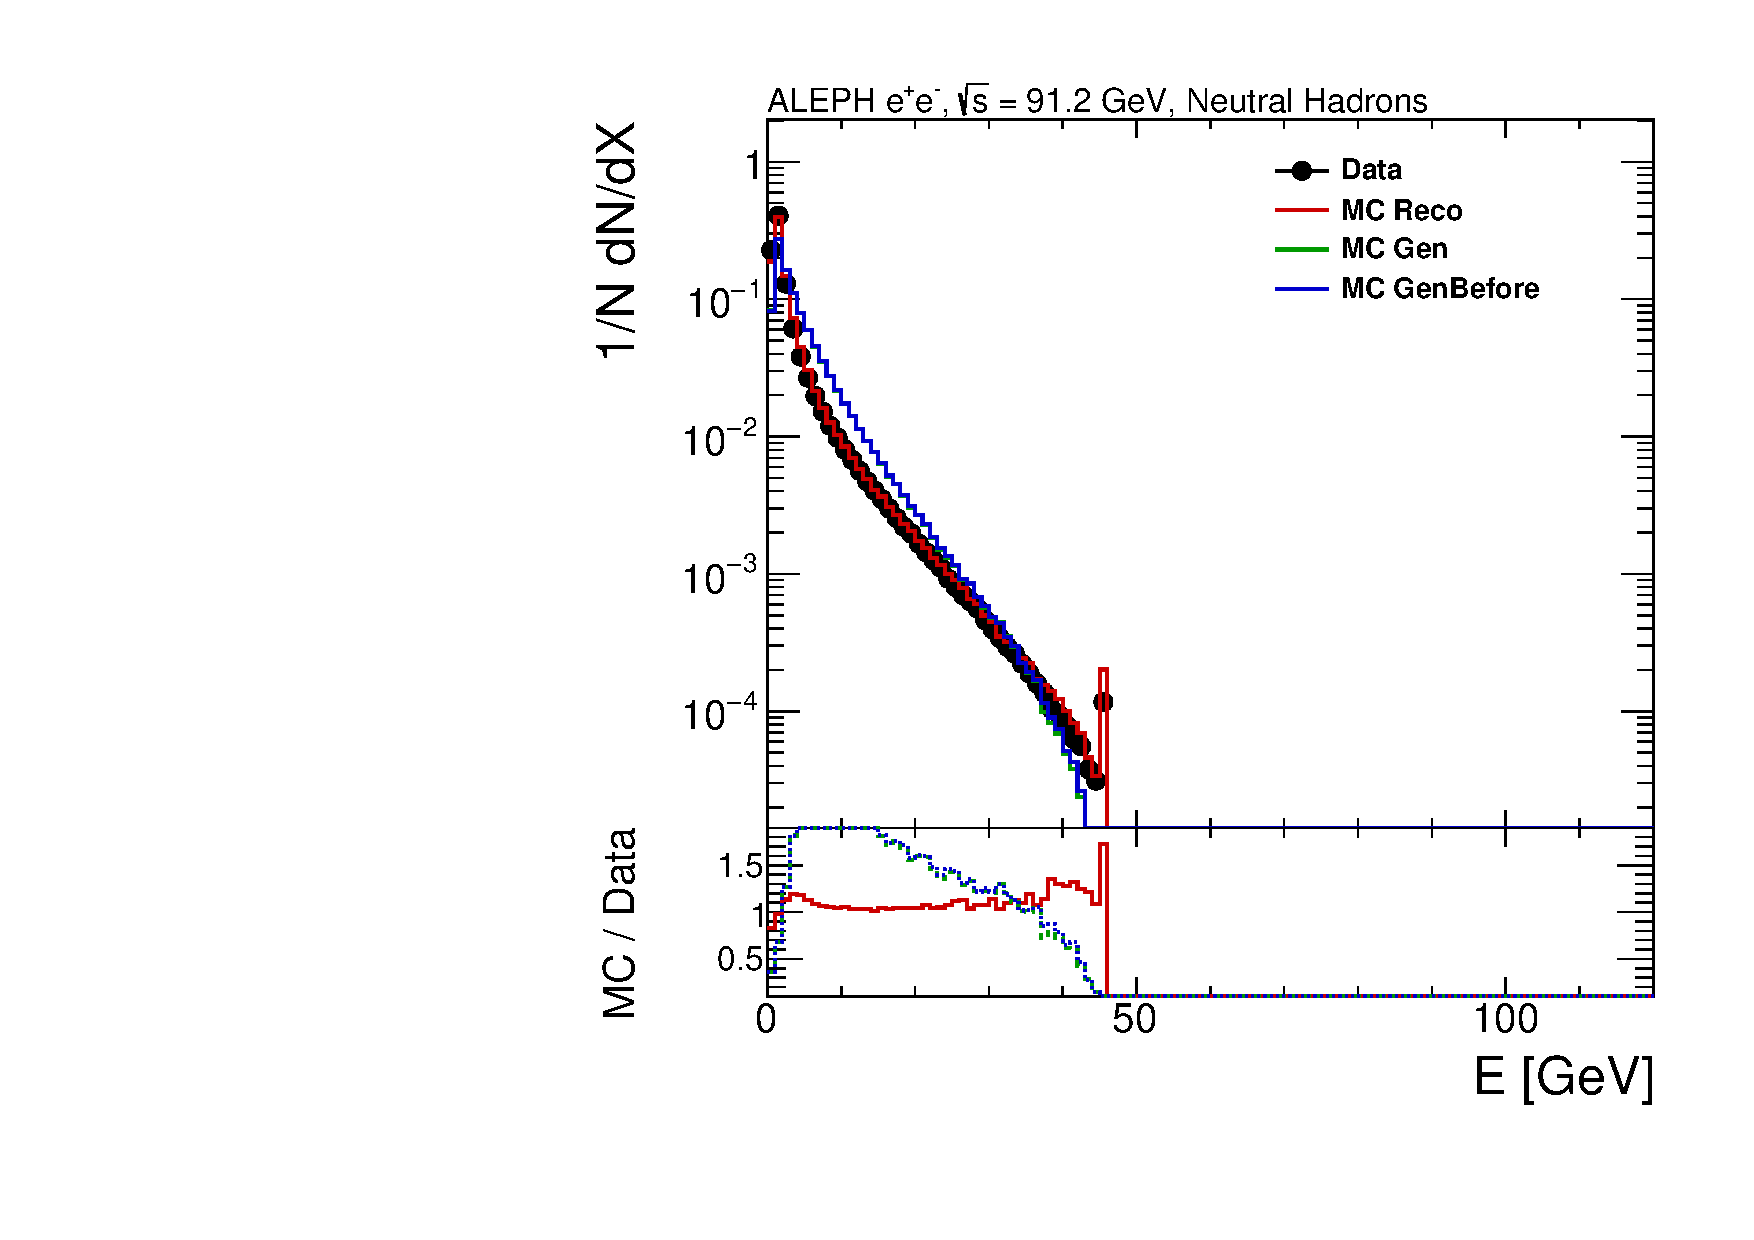
\includegraphics[width=0.495\textwidth]{figures/pwflag5_energy.pdf}
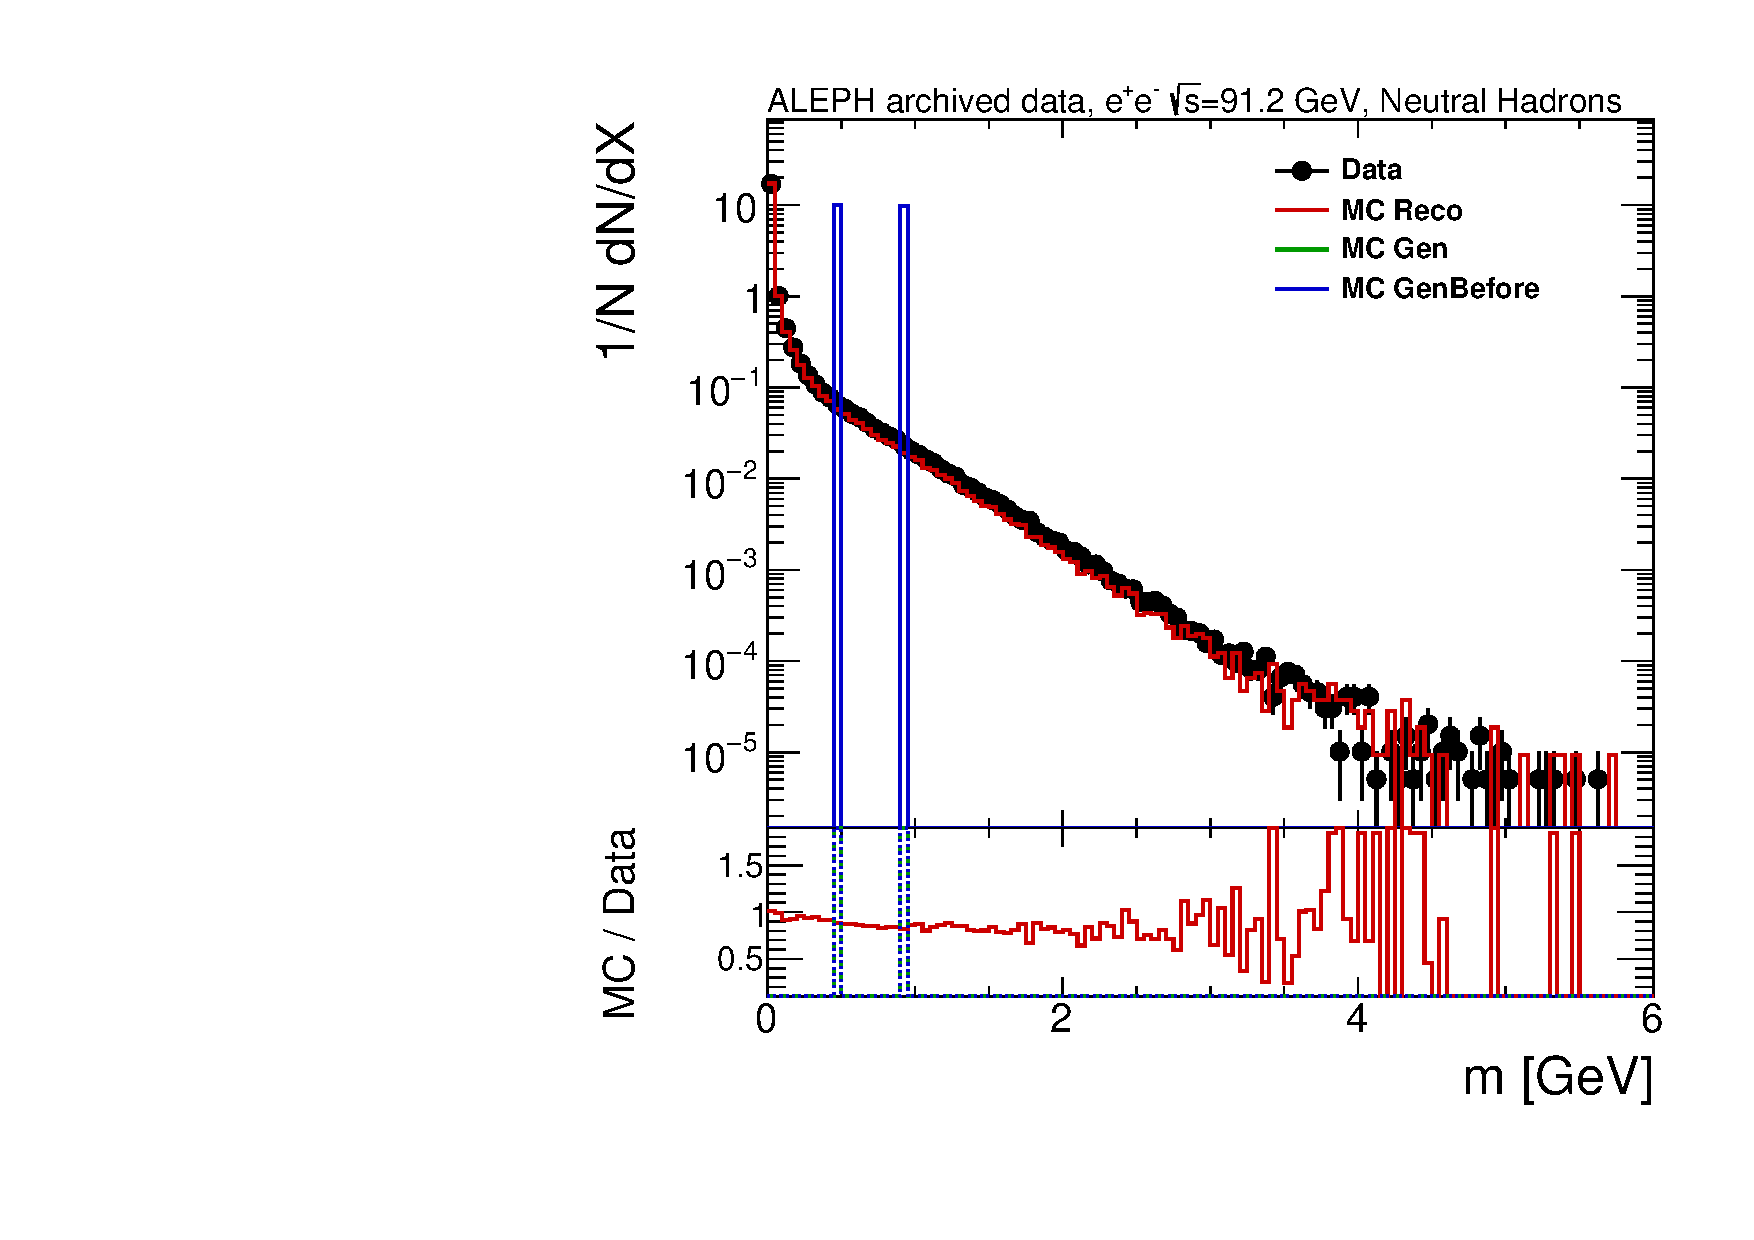
\includegraphics[width=0.495\textwidth]{figures/pwflag5_mass.pdf}
\caption{Complete \texttt{pwflag}=5 kinematic set.}
\label{fig:pwflag5_full}
\end{figure}

\FloatBarrier

\begin{figure}[t!]
\centering
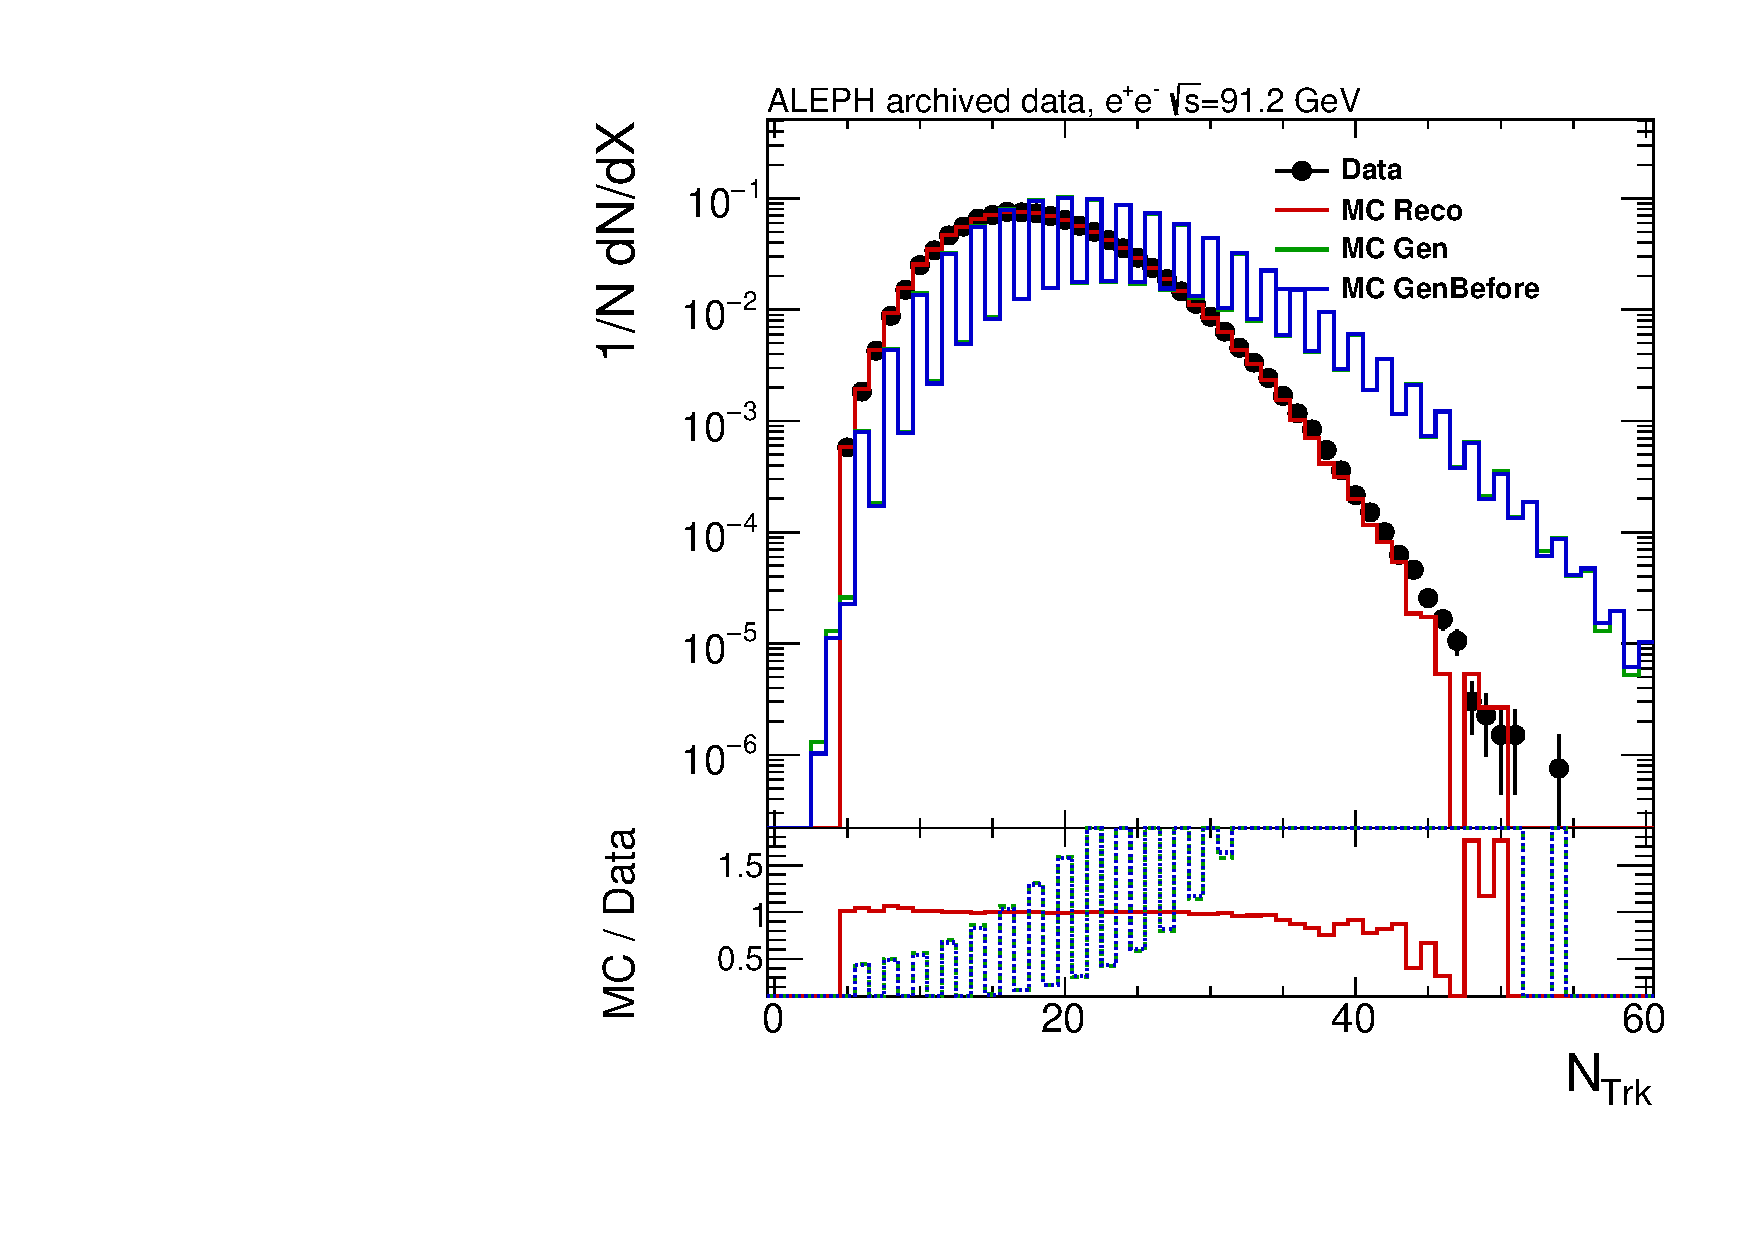
\includegraphics[width=0.495\textwidth]{figures/ntrk.pdf}
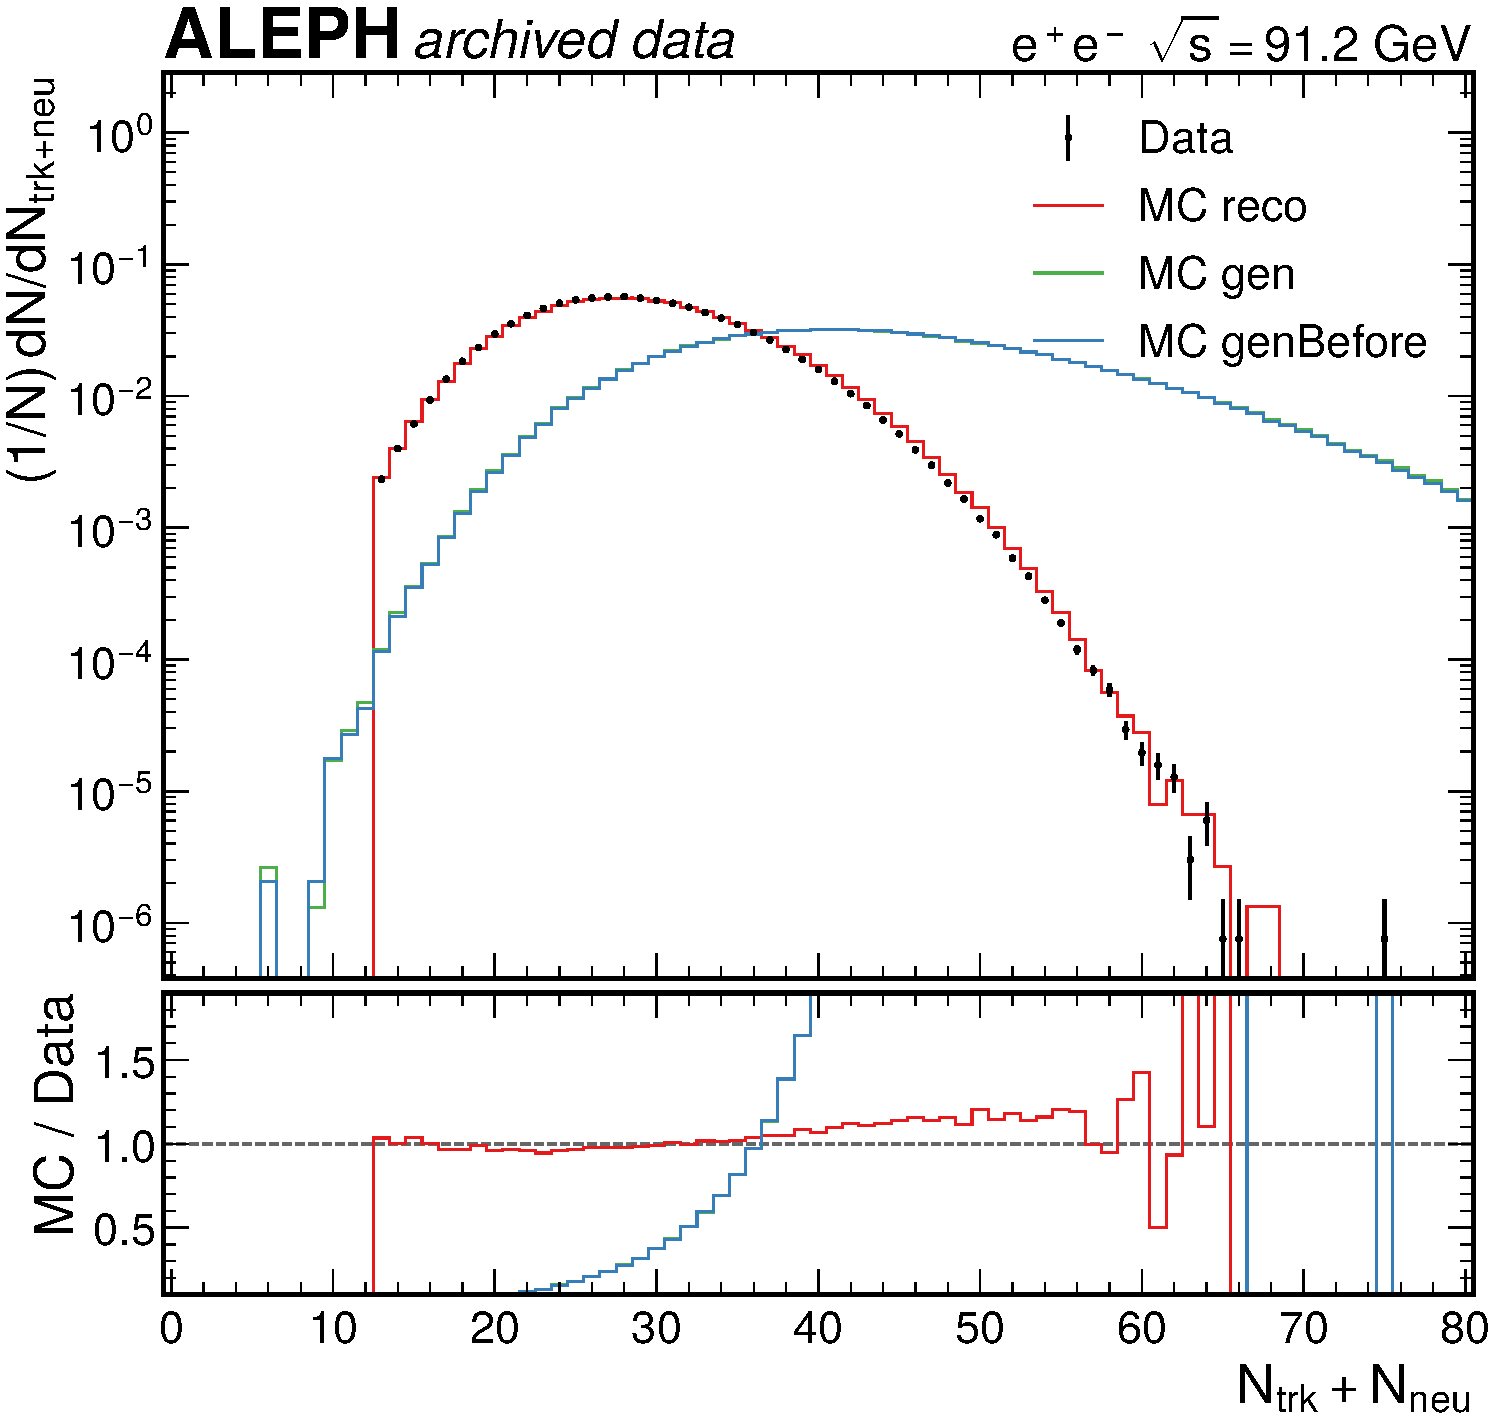
\includegraphics[width=0.495\textwidth]{figures/ntrkPlusNeu.pdf}
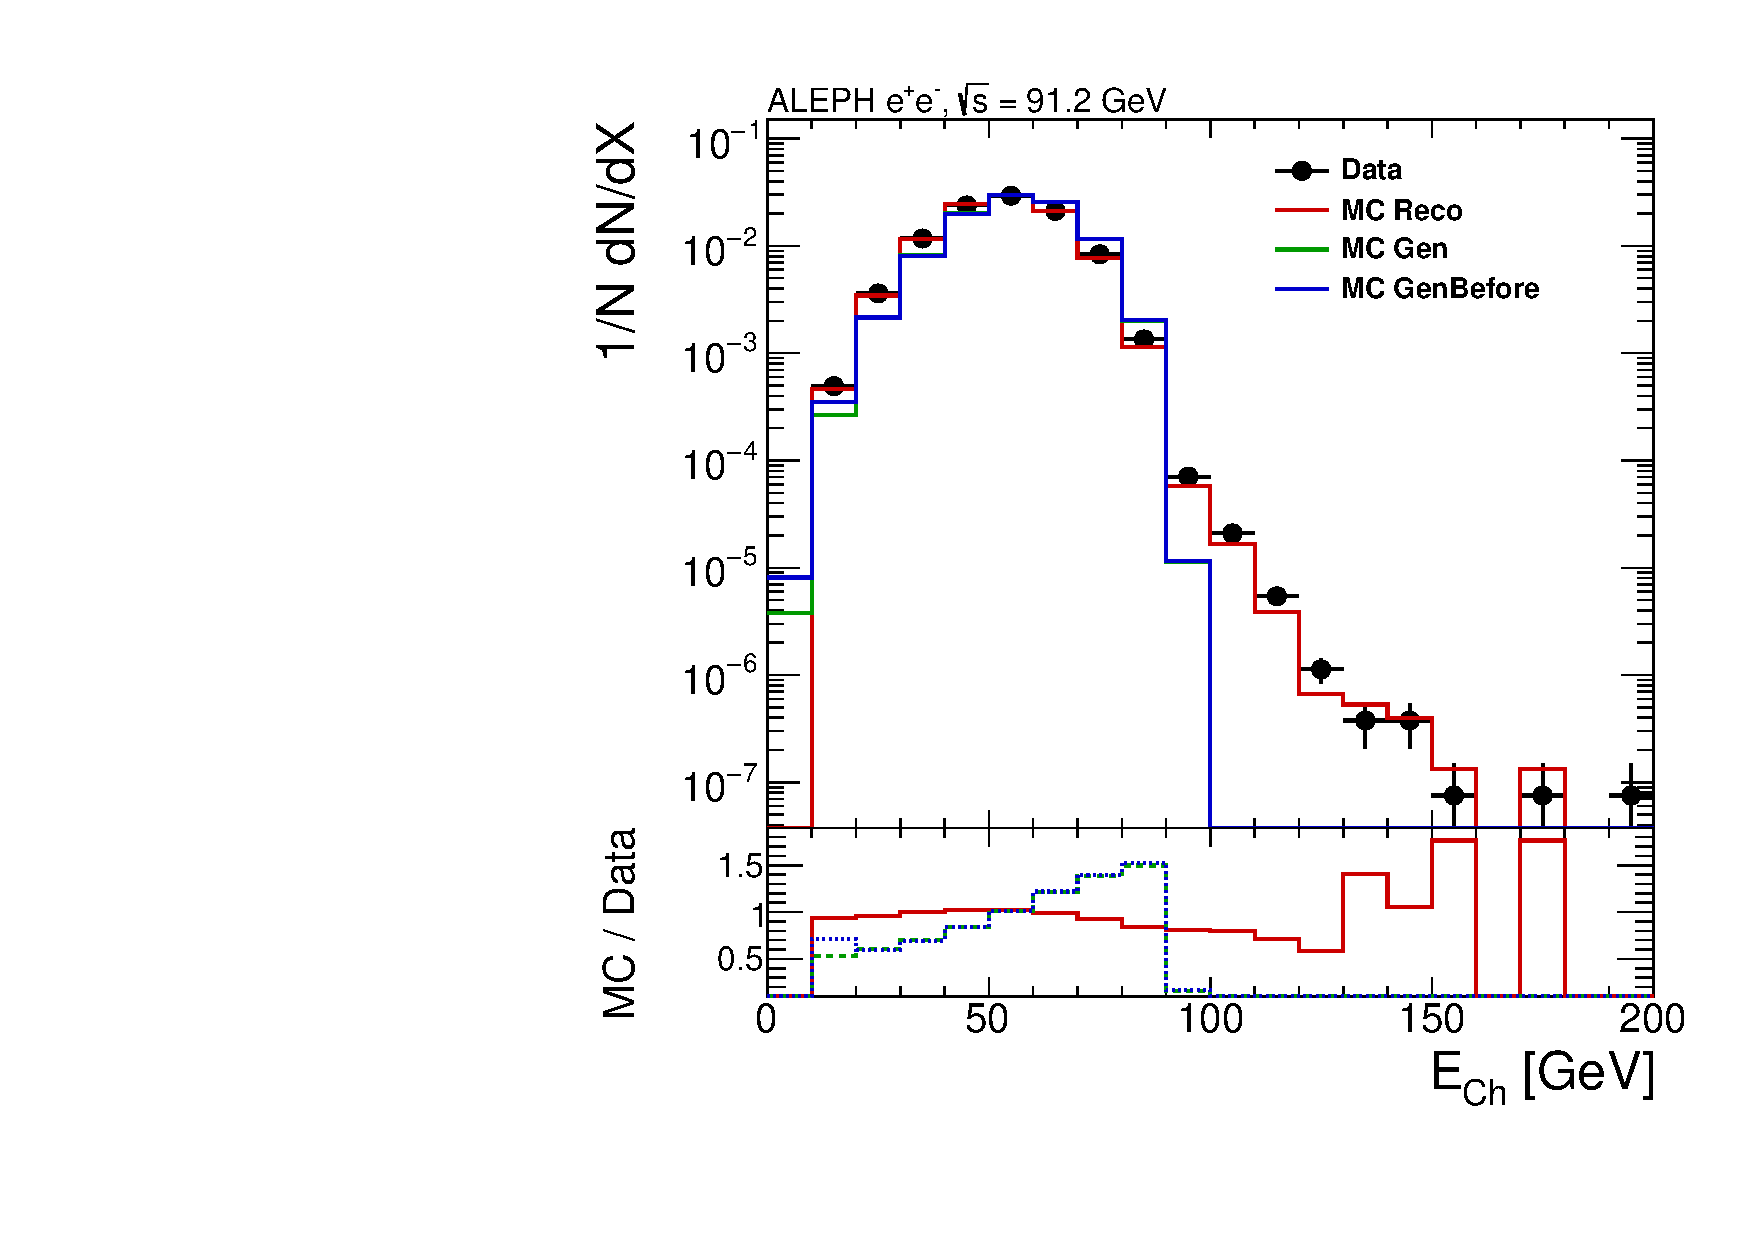
\includegraphics[width=0.495\textwidth]{figures/eCh.pdf}
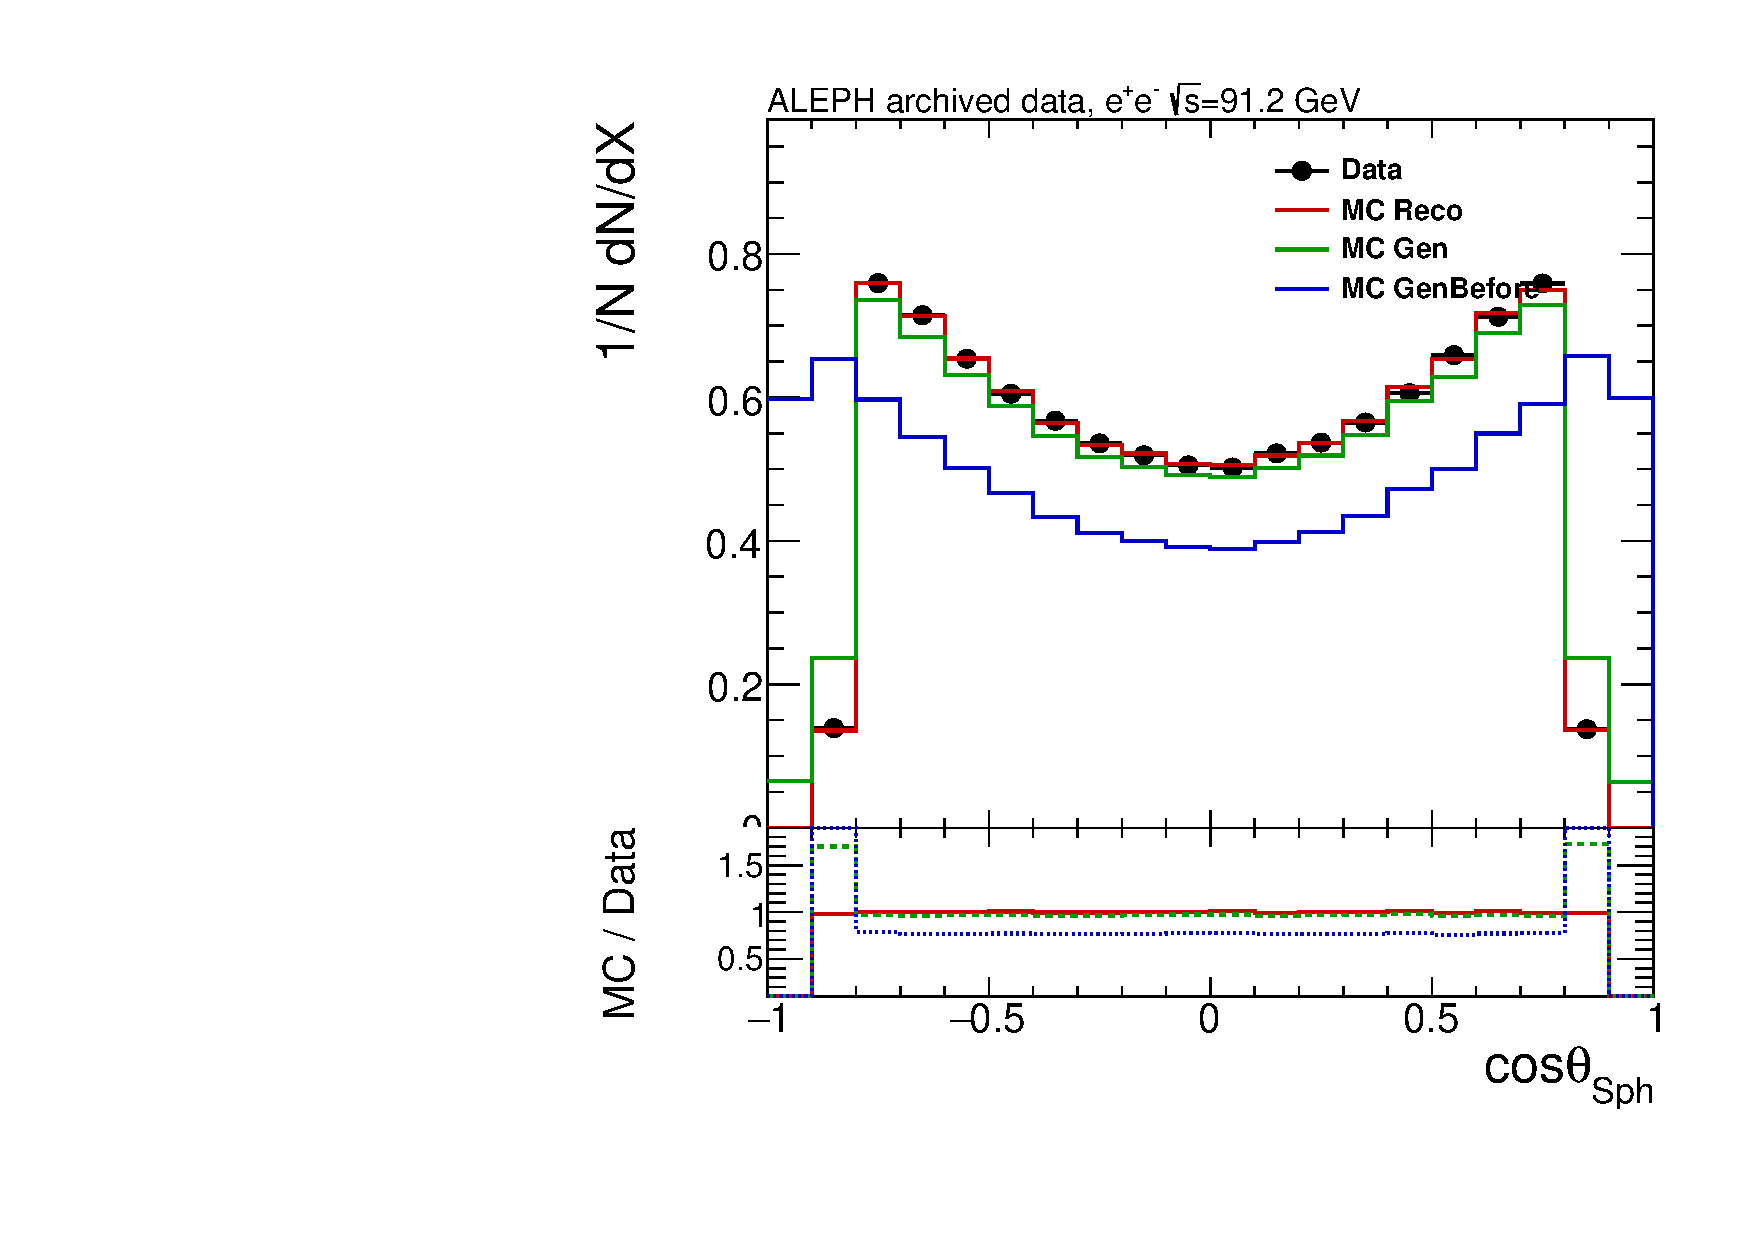
\includegraphics[width=0.495\textwidth]{figures/cosThetaSph.pdf}
\caption{Event-level observables used in the nominal hadronic selection; legends include detector-level data/MC and generator-level references. The MC\,Gen and MC\,GenBefore ratios display an even-odd staggering: generator-level charged multiplicity has an approximately 6:1 even-to-odd ratio (arising from the Z-decay net-charge constraint and the specific ALEPH Pythia~6 particle record), while reconstruction efficiency losses smear individual tracks one at a time and equalise the even/odd balance in data and MC\,Reco.
MC\,Reco is the relevant comparison for the analysis.}
\label{fig:event_selection_observables}
\end{figure}

\FloatBarrier

% \subsection{Event-level selection observables}

% The event-level panels close the logic between object-level selections and the final sample
% entering event-shape reconstruction. $N_{\mathrm{trk}}$ and
% $N_{\mathrm{trk}}+N_{\mathrm{neu}}$ test whether multiplicity thresholds sculpt data and MC in a
% consistent way; this is critical because those same multiplicities enter hadronic-event
% preselection and determine which events contribute to response filling. $E_{\mathrm{Ch}}$ checks
% charged-energy modeling near the hadronic-selection boundary at 15 GeV, and
% $\cos\theta_{\mathrm{Sph}}$ tests whether accepted event topology is similarly contained in
% detector acceptance for data and MC.

% The \texttt{tgen} and \texttt{tgenBefore} samples receive the same particle-level treatment and differ
% only in which events are retained: \texttt{tgen} holds the generator record of the events
% written to the reconstructed after-cut sample, \texttt{tgenBefore} that of all generated
% events, so \texttt{tgen} is a subset. The kinematic selections of
% Sec.~\ref{sec:object_selection} are applied at detector level only, and no additional
% cleaning is applied at generator level. The events
% missing from \texttt{tgen} are removed almost entirely by polar-angle acceptance rather than
% by particle content, so the normalized multiplicity and charged-energy spectra coincide
% through the bulk, separating only in the sparse low-$E_{\mathrm{Ch}}$ tail near the
% charged-energy boundary, and $\cos\theta_{\mathrm{Sph}}$ is the one panel where the curves
% clearly differ. Both generator-level curves also show an even--odd modulation in
% $N_{\mathrm{trk}}$: the charged multiplicity shares the parity of the summed charge of the
% counted particles, which charge conservation makes vanish for most generated events. The
% modulation is absent at detector level, where charged-track inefficiency randomizes the
% parity.

% Overall agreement in the high-statistics regions supports the response-model baseline used for IBU. The visible differences are concentrated in lower-populated tails and near selection boundaries, where statistical fluctuations and detector-response limitations are expected to be larger. These regions are not ignored: their impact is propagated through the experimental systematic program and is reflected in the final uncertainty decomposition.

% \FloatBarrier
% \clearpage

\section{Analysis method}
\label{sec:method}

\subsection{Observable definition and construction}

The thrust observable is defined as~\cite{PhysRevLett.39.1587}
\begin{equation}
T = \max_{\hat{n}} \frac{\sum_i |\vec{p}_i \cdot \hat{n}|}{\sum_i |\vec{p}_i|},
\end{equation}
with all selected charged and neutral reconstructed objects from Sec.~\ref{sec:event_selection} entering the sum. The thrust is built using selected charged and neutral particles. Those objects are input to an optimization algorithm that iteratively determines the thrust axis. The algorithm we use is a clone of the \textsc{Herwig++} implementation~\cite{Brandt:1978zm, B_hr_2008, BUCKLEY20132803, rivet_thrust}, which is an exact calculation rather than one based on heuristics as is done by others~\cite{Belle2Thrust}. The resolution is characterized using matched reco--gen event pairs. Figure~\ref{fig:thrust_resolution_2d} shows $(T_{\mathrm{reco}} - T_{\mathrm{gen}})$ as a function of $T_{\mathrm{gen}}$. The resolution narrows toward $T\to1$. To enable direct comparison, our work adopts the same binning as the previous ALEPH analyses~\cite{Barate:1996fi, Heister:2003aj}, with 42 uniform bins over $0.58 \le T < 1.0$ (bin width $\Delta T = 0.01$).

\begin{figure}[ht!]
\centering
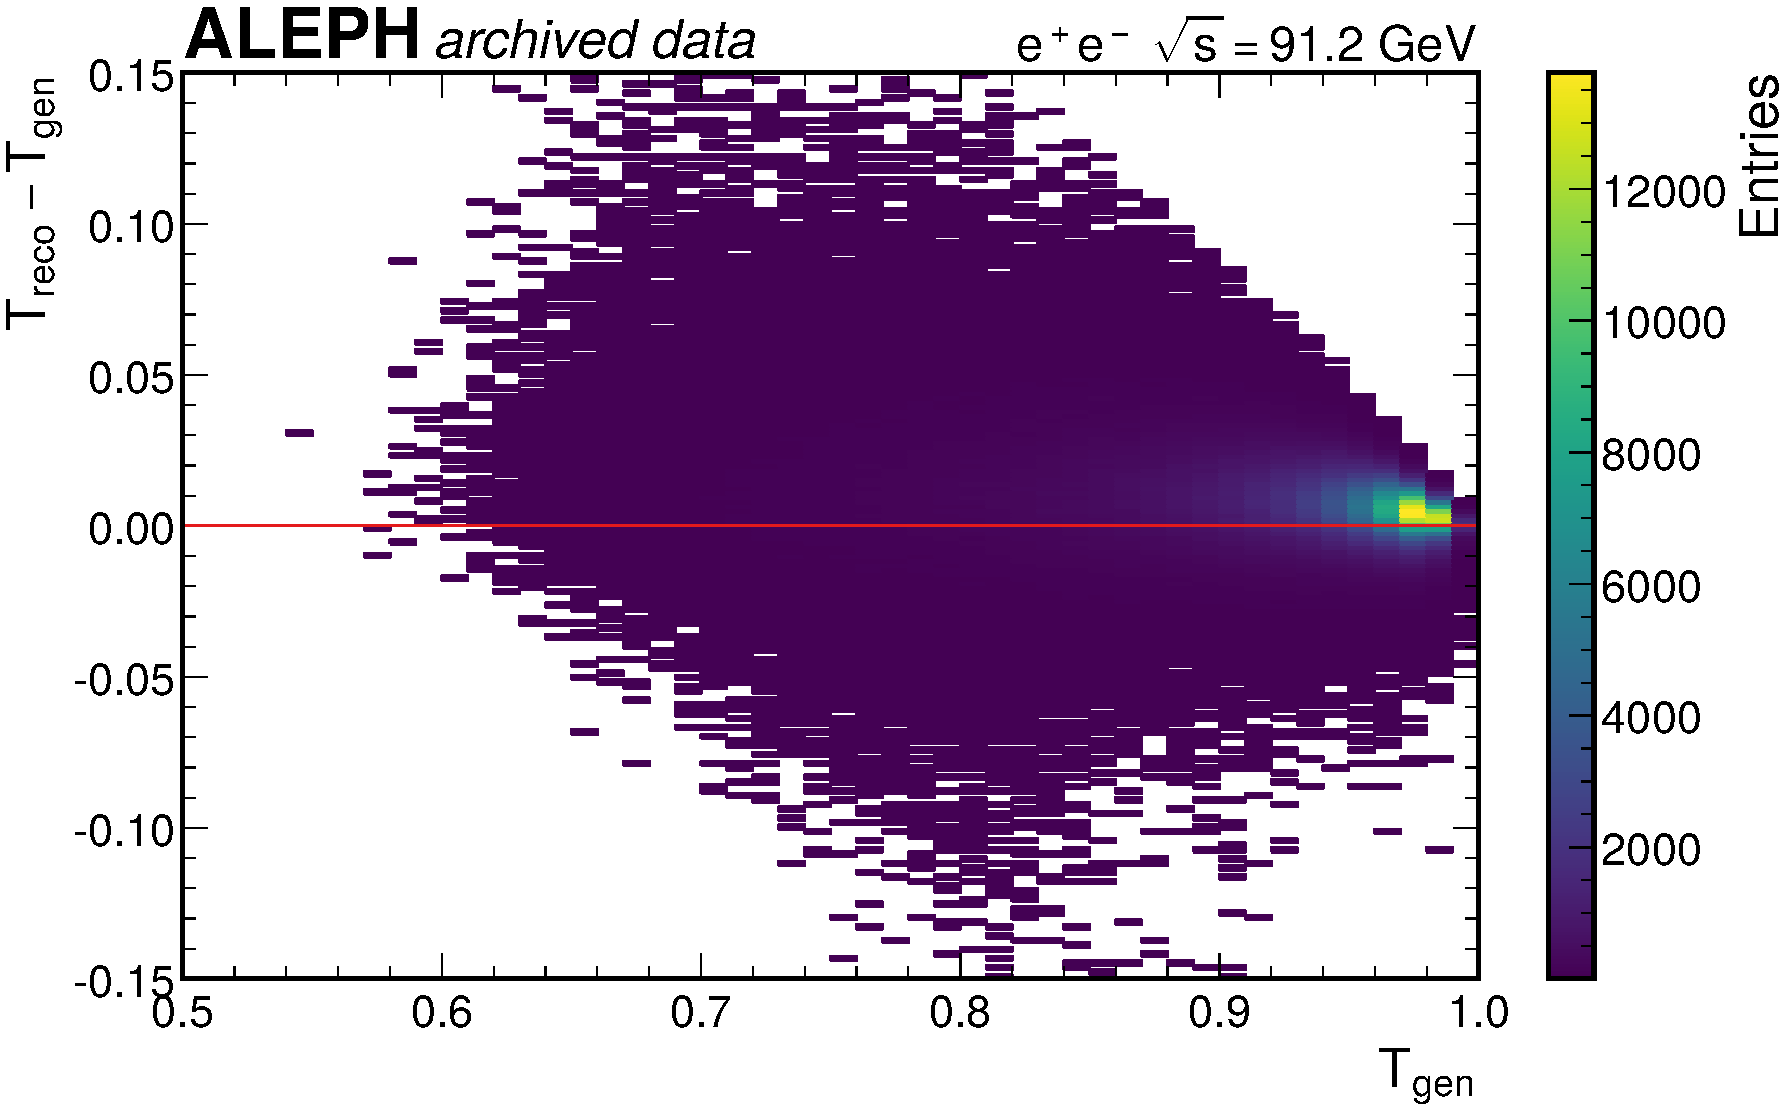
\includegraphics[width=0.85\textwidth]{figures/thrust_resolution_2d.pdf}
\caption{Thrust resolution $(T_{\mathrm{reco}}-T_{\mathrm{gen}})$ versus $T_{\mathrm{gen}}$ for matched MC event pairs.}
\label{fig:thrust_resolution_2d}
\end{figure}

\subsection{Unfolding setup and regularization choice}

Detector correction is performed with the IBU method of D'Agostini~\cite{DAgostini:1994zf,dagostini2010improvediterativebayesianunfolding}, as implemented in RooUnfold~\cite{Adye:2011gm},
\begin{equation}
U_j^{(n+1)} = \frac{1}{\epsilon_j}\sum_i M_i\,\frac{R_{ij}\,\pi_j^{(n)}}{\sum_k R_{ik}\,\pi_k^{(n)}},
\end{equation}
where $M_i$ is the measured detector-level spectrum, $R_{ij}$ is the response, and $\pi_j^{(n)}$ is the iteration prior. The prior for the first iteration is taken as the generator-level MC truth distribution $\pi_j^{(0)} = N_{\mathrm{gen}}(j)$, the standard RooUnfold default. This choice initializes the unfolding close to the expected truth shape and avoids any flat-prior amplification of high-frequency fluctuations in the first iteration. The response matrix is filled with MC events that pass the detector-level selection and the corresponding generator-level event as shown in Figure~\ref{fig:response_matrices_nominal}. A selected event whose reconstructed thrust falls outside the unfolding range enters instead through RooUnfold's miss term, which supplies the efficiency factor $1/\epsilon_j$ appearing below.

\begin{figure}[ht!]
\centering
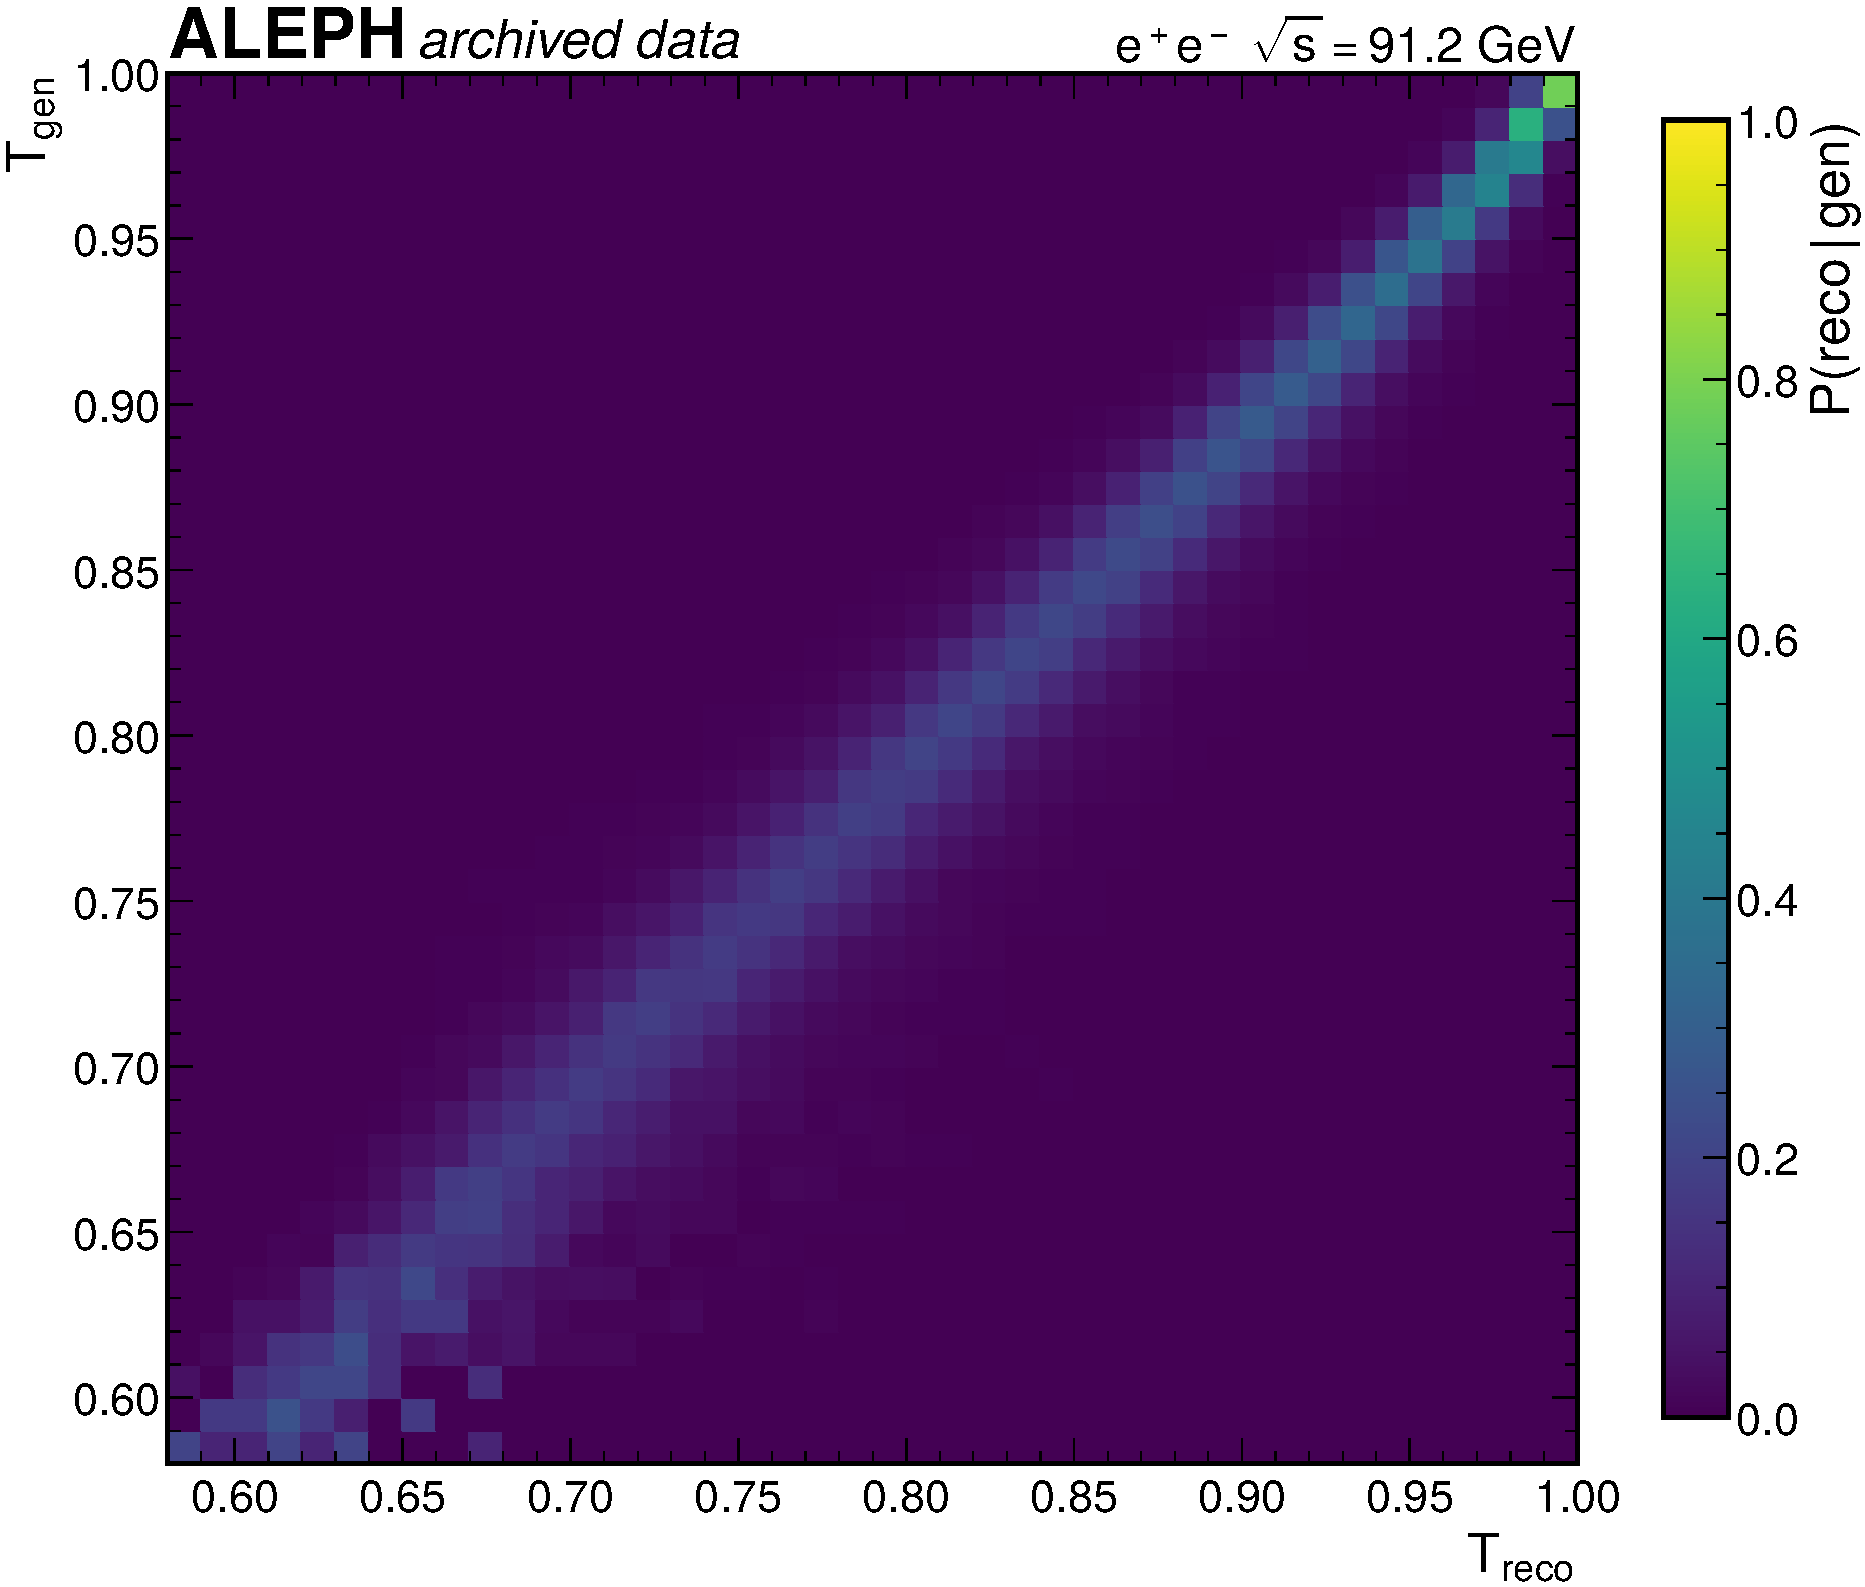
\includegraphics[width=0.85\textwidth]{figures/matrix_response_probability.pdf}
\caption{Nominal response probability matrix for thrust.}
\label{fig:response_matrices_nominal}
\end{figure}

The IBU regularization term for the number of iterations is kept at a nominal value of $N_{\mathrm{iter}}=5$ as found by previous studies~\cite{Badea:2019vey}, with $N_{\mathrm{iter}}=4$ and $6$ propagated as unfolding-regularization systematic branches.
The iteration-choice diagnostics, including refolded spectra at $N=4,5,6,10,100$ compared with detector-level data, confirm that the closure-shape $\chi^2/\mathrm{ndf}$ is stable for $N_{\mathrm{iter}}\in\{4,5,6\}$. The spread in the unfolded thrust spectrum across this range is below $1\%$ in 37 of the 42 reported bins (median $0.3\%$), rising to at most $6.6\%$ near the two-jet edge ($T\lesssim0.62$) where the steeply falling spectrum amplifies regularization sensitivity.

The response matrix has a diagonal fraction of $f_{\mathrm{diag}}=0.33$, meaning approximately two-thirds of events migrate out of their generated thrust bin at reconstruction level. This level of bin-to-bin migration is expected for thrust at ALEPH given the finite charged-particle momentum resolution and the sensitivity of thrust to soft particles near the event boundary. It implies that the unfolding correction is non-trivial and that the choice of regularization strength meaningfully affects the result. This also motivates the need to measure the final bin-by-bin correlation to assess the overall statistical strength.

The miss term, the generator-level events with no matched reconstructed counterpart, is
shown in Fig.~\ref{fig:miss_term_efficiency}. These are events that fail the reco-level hadronic event selection despite being generated within the fiducial volume. The miss rate is concentrated at low thrust ($T\lesssim0.7$) and in events with low charged multiplicity, consistent with the hadronic event selection removing poorly reconstructed events. RooUnfold accounts for miss events via \texttt{response.Miss($x_{\mathrm{gen}}$)}, which corrects the unfolded spectrum for this acceptance effect.

\begin{figure}[ht!]
\centering
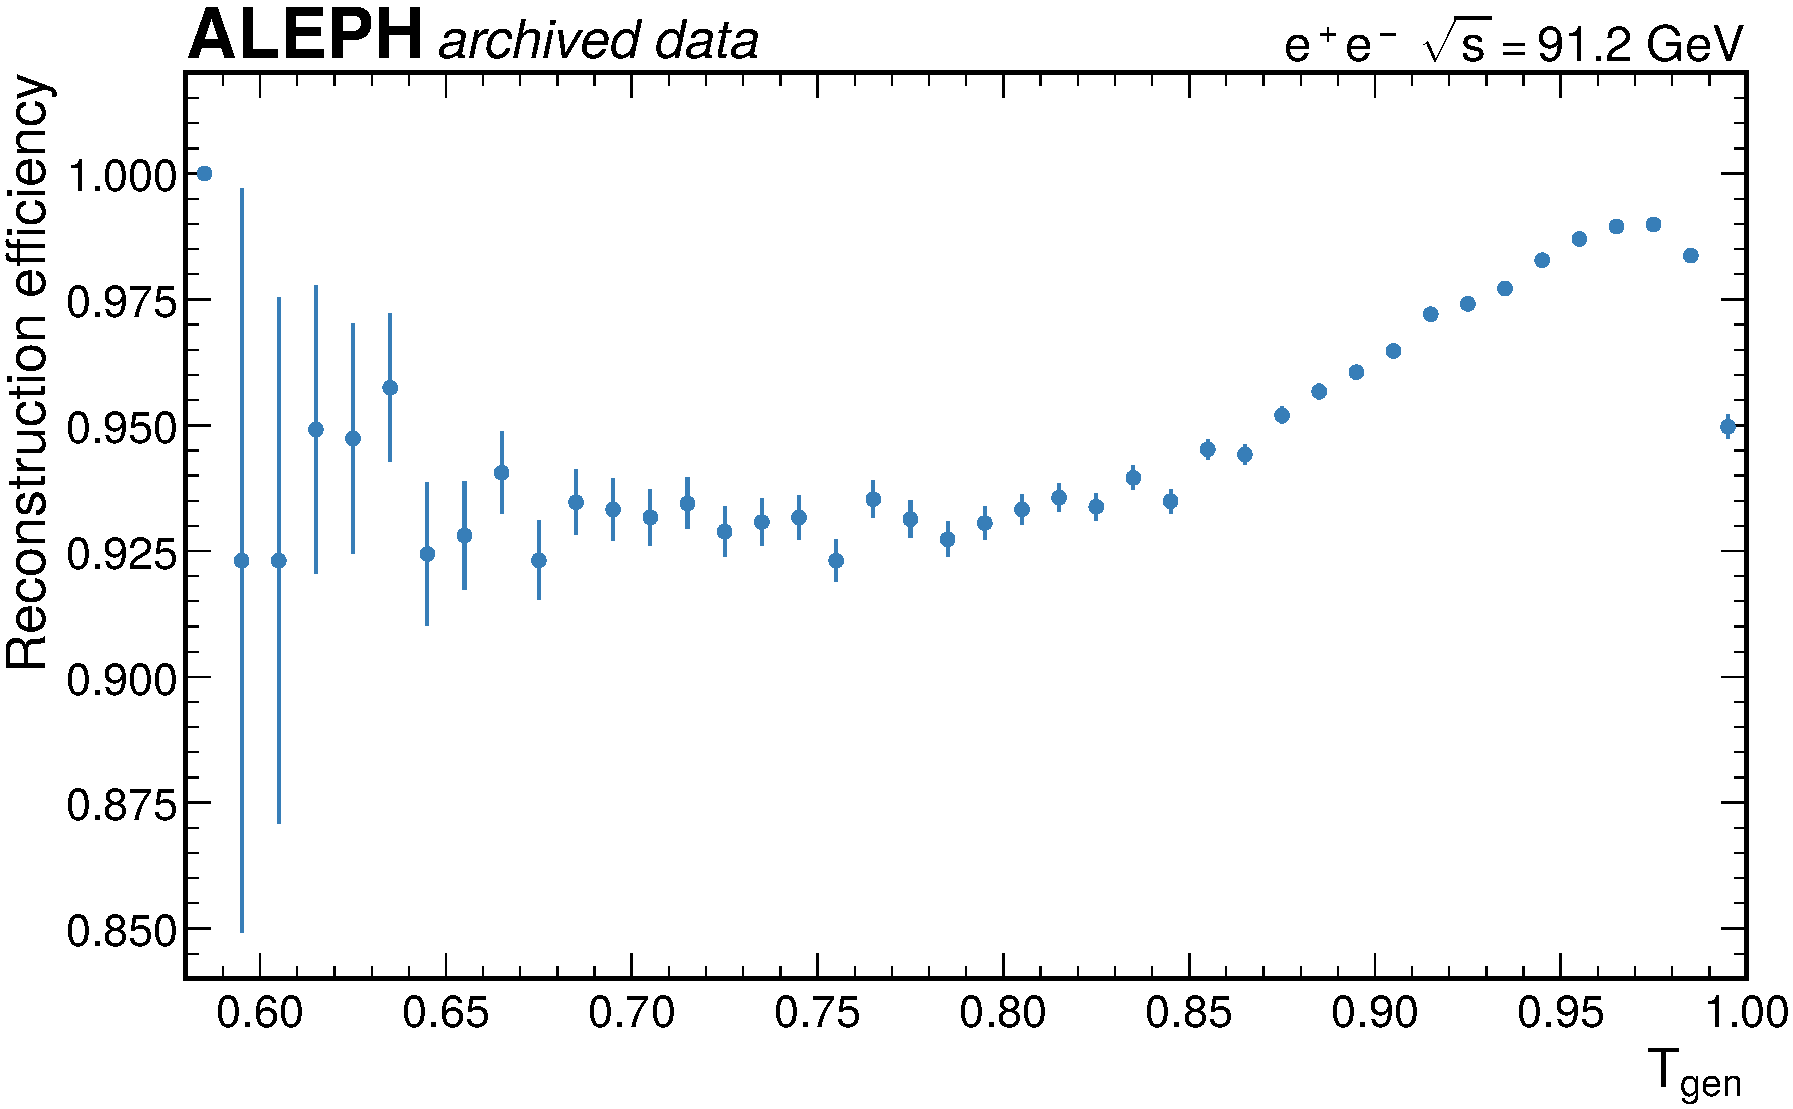
\includegraphics[width=0.49\textwidth]{figures/miss_term_efficiency.pdf}
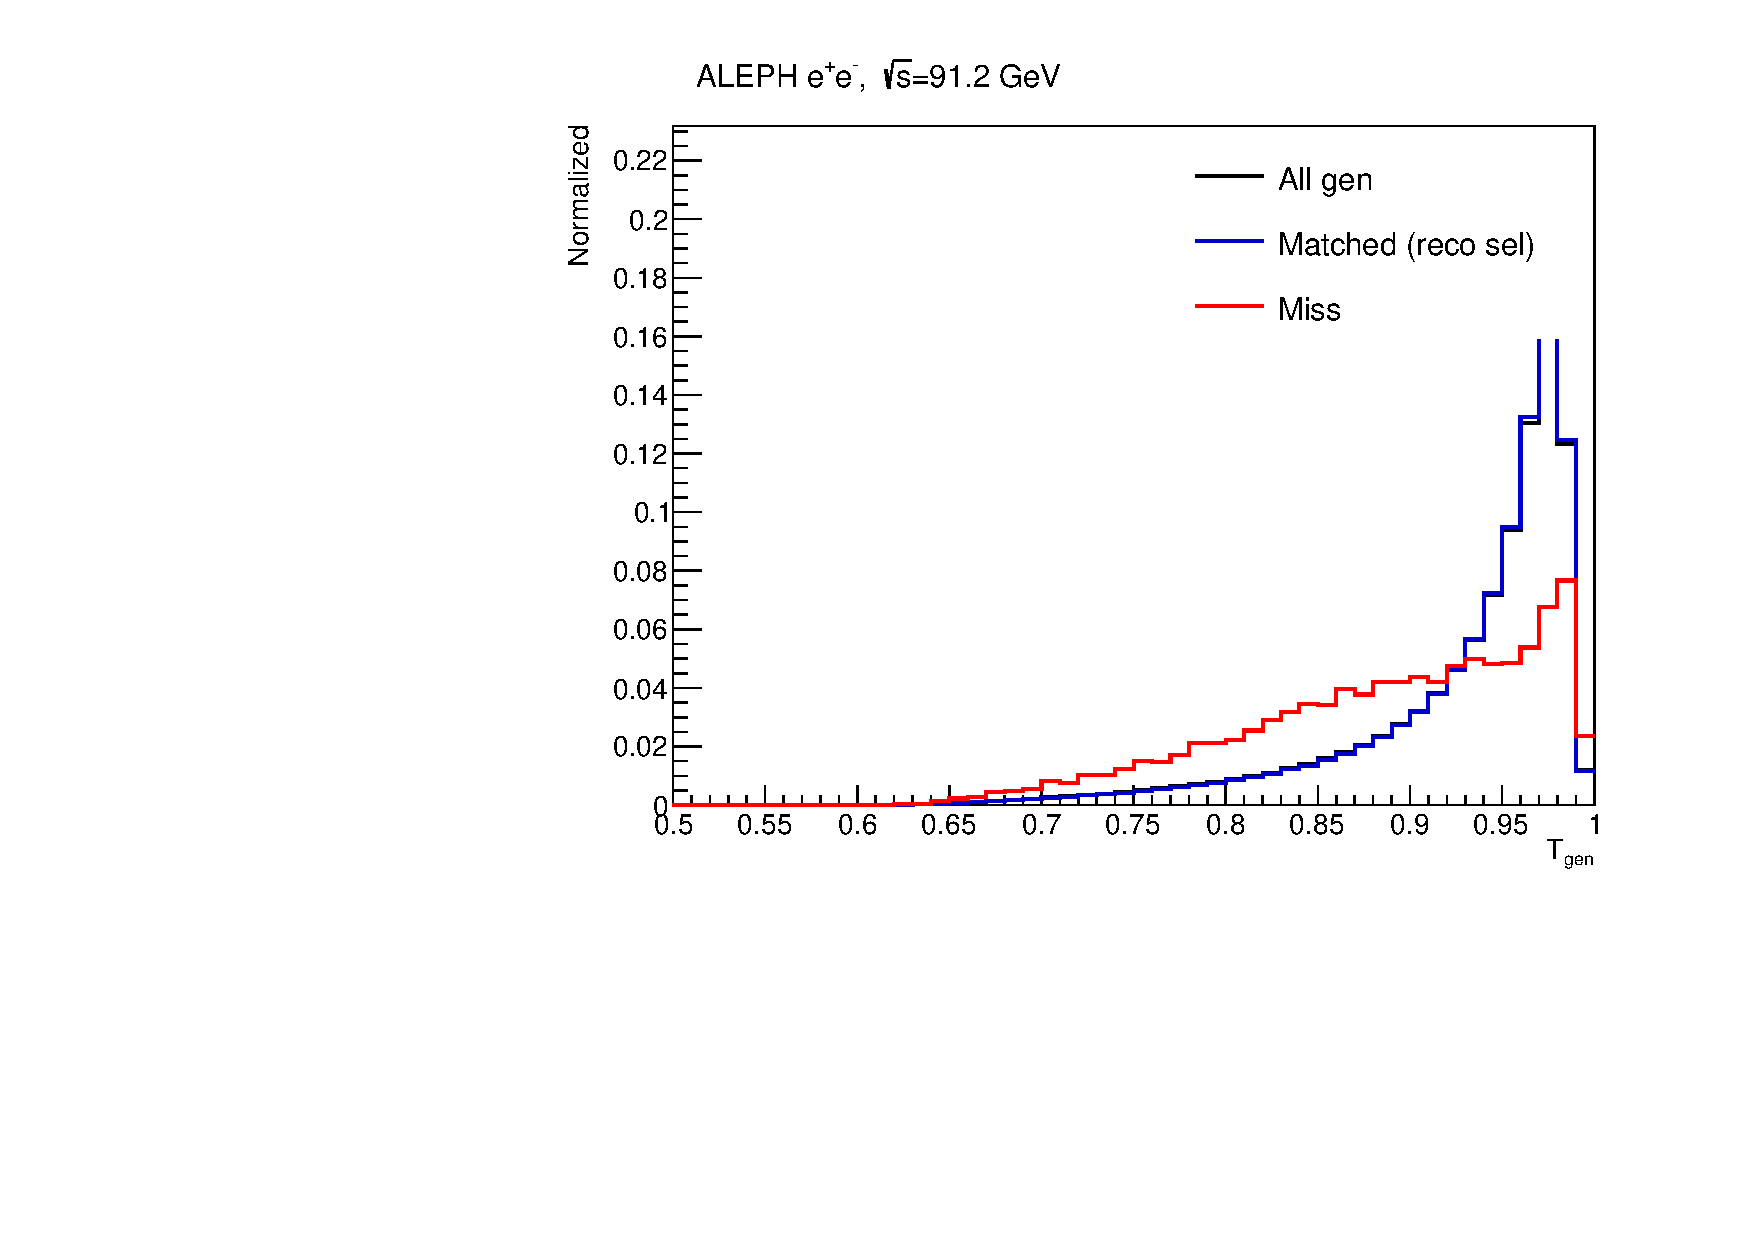
\includegraphics[width=0.49\textwidth]{figures/miss_term_thrust.pdf}
\caption{Left: reco efficiency (matched/all gen) as a function of $T_{\mathrm{gen}}$,
with binomial uncertainties. Right: thrust distributions for all gen, matched, and miss
events (normalized to unit area). Miss events are concentrated at low thrust and low
multiplicity, consistent with events failing the hadronic event selection.}
\label{fig:miss_term_efficiency}
\end{figure}

\subsection{Hadronic and QED ISR correction}
\label{sec:corrections_and_cov}

After unfolding, two multiplicative corrections are applied. A correction for the hadronic event-selection,
\begin{equation}
C_{\mathrm{had}}(j) = \frac{N_{\mathrm{genBefore}}(j)}{N_{\mathrm{gen}}(j)},
\end{equation}
accounts for the efficiency of the selection at the generator level. The correction factor is derived from the archived \textsc{Pythia}~6 sample~\cite{Sjostrand:2000wi} and is applied so that the final spectrum restores the yield lost by the hadronic selection.

Then a correction for electromagnetic (QED) initial-state radiation (ISR) is applied,
\begin{equation}
C_{\mathrm{ISR}}(j) = \frac{N^{\mathrm{gen}}_{\mathrm{no\,ISR}}(j)}{N^{\mathrm{gen}}_{\mathrm{ISR}}(j)}.
\end{equation}
This factor is applied to enable comparisons with state-of-the-art theory calculations which do not include QED ISR. The correction is derived from standalone \textsc{Pythia}~8.317 samples generated with ISR switched off and on~\cite{Bierlich:2022pfr}. \textsc{Pythia}~8.317 is chosen here for simplicity; a higher-order generator such as \textsc{KKMCee}~5.00.02 would be preferred for a full thrust measurement~\cite{Jadach:2022mbe}. The ratio histograms are pre-computed once into a cache file and applied identically to the nominal and all systematic variation branches, so that the ISR correction cancels in the systematic shifts and its residual uncertainty (from finite MC statistics on the ratio) is propagated as a separate component $\Delta_{\mathrm{ISR}}$ (Sec.~\ref{sec:isr_uncertainty}).

For the nominal result, the data statistical covariance is computed by RooUnfold using analytical error propagation (\texttt{RooUnfold::kCovariance}), which propagates Poisson uncertainties in the measured data through the IBU iteration chain without toy MC sampling. The response matrix's own finite statistics are not included by that call and are propagated separately by a Poisson bootstrap over the simulated events, as described in Sec.~\ref{sec:stat_uncertainty}. The resulting covariance matrices are read from the unfolding output and transformed to the normalized differential-thrust basis used in this work. Non-statistical component covariances are built with a configurable model, and all covariance products are exported over the reported bins.

\section{Systematic uncertainties}
\label{sec:systematics}

% Systematic variations are propagated by rerunning the full unfolding chain for each
% variation and comparing to the nominal unfolded result. For each source $v$, the
% signed bin-wise shift is
% \begin{equation}
% \delta_v(j)=\frac{U_v(j)-U_{\mathrm{nom}}(j)}{U_{\mathrm{nom}}(j)}.
% \end{equation}
% The sources are grouped into seven independent components

Systematic uncertainties arise from several components: data statistical, MC statistical, unfolding-regularization, experimental variations, theory unfolding prior, hadronic event-selection correction, and ISR correction. The sections below describe each component.

\subsection{Statistical uncertainty}
\label{sec:stat_uncertainty}

The data statistical uncertainty is propagated analytically by RooUnfold through the IBU iteration chain, without toy-MC sampling, yielding a full statistical covariance matrix $\mathrm{Cov}^{(\mathrm{stat})}_{ij}$. The per-bin fractional uncertainty $\Delta_{\mathrm{stat}}(j)=\sqrt{\mathrm{Cov}^{(\mathrm{stat})}_{jj}}/U_j^{\mathrm{corr}}$ is typically below $2\%$ in the central range and nearly uniform across the spectrum. The uncertainty is shown in Figure~\ref{fig:unc_comp_stat_iter}.

MC statistical uncertainties enter the budget through the two corrections derived from finite simulated samples: the MC statistical uncertainty of the ISR-off and ISR-on samples is propagated onto $C_{\mathrm{ISR}}(j)$, and the archived-MC statistical uncertainty of $N_{\mathrm{genBefore}}$ and $N_{\mathrm{gen}}$ is propagated onto the hadronic event-selection correction $C_{\mathrm{had}}(j)$. The finite statistics of the response matrix itself are propagated separately, by giving every matched simulated event a Poisson weight and re-unfolding the data over 200 such replicas; the sample covariance of the resulting spectra is taken as $\mathrm{Cov}^{(\mathrm{MCstat})}_{ij}$. This is required because \texttt{RooUnfold::kCovariance} transports the measured data covariance only, and because the simulated sample is smaller than the data sample, so the response statistical term exceeds the data statistical term in every bin.

\subsection{Unfolding regularization uncertainty}
\label{sec:stat_uncertainty}

The unfolding regularization uncertainty is closely related: two additional unfolding passes at $N_{\mathrm{iter}}=4$ and $N_{\mathrm{iter}}=6$ quantify the sensitivity of the result to the regularization choice. The iteration envelope $\Delta_{\mathrm{iter}}(j)=\max(|\delta_{\mathrm{iter4}}(j)|,|\delta_{\mathrm{iter6}}(j)|)$
is sub-percent in the bulk of the spectrum, confirming that the nominal $N_{\mathrm{iter}}=5$ sits on a stable plateau and that regularization is not a limiting source of uncertainty. Figure~\ref{fig:unc_comp_stat_iter} shows the
signed per-bin shifts for both components across the measurement range. The iteration shifts change sign across the range because $N_{\mathrm{iter}}=4$ and $6$ bracket the nominal, and the bin-to-bin alternation at low thrust reflects the anti-correlation that regularization induces between neighboring bins.

\begin{figure}[ht!]
\centering
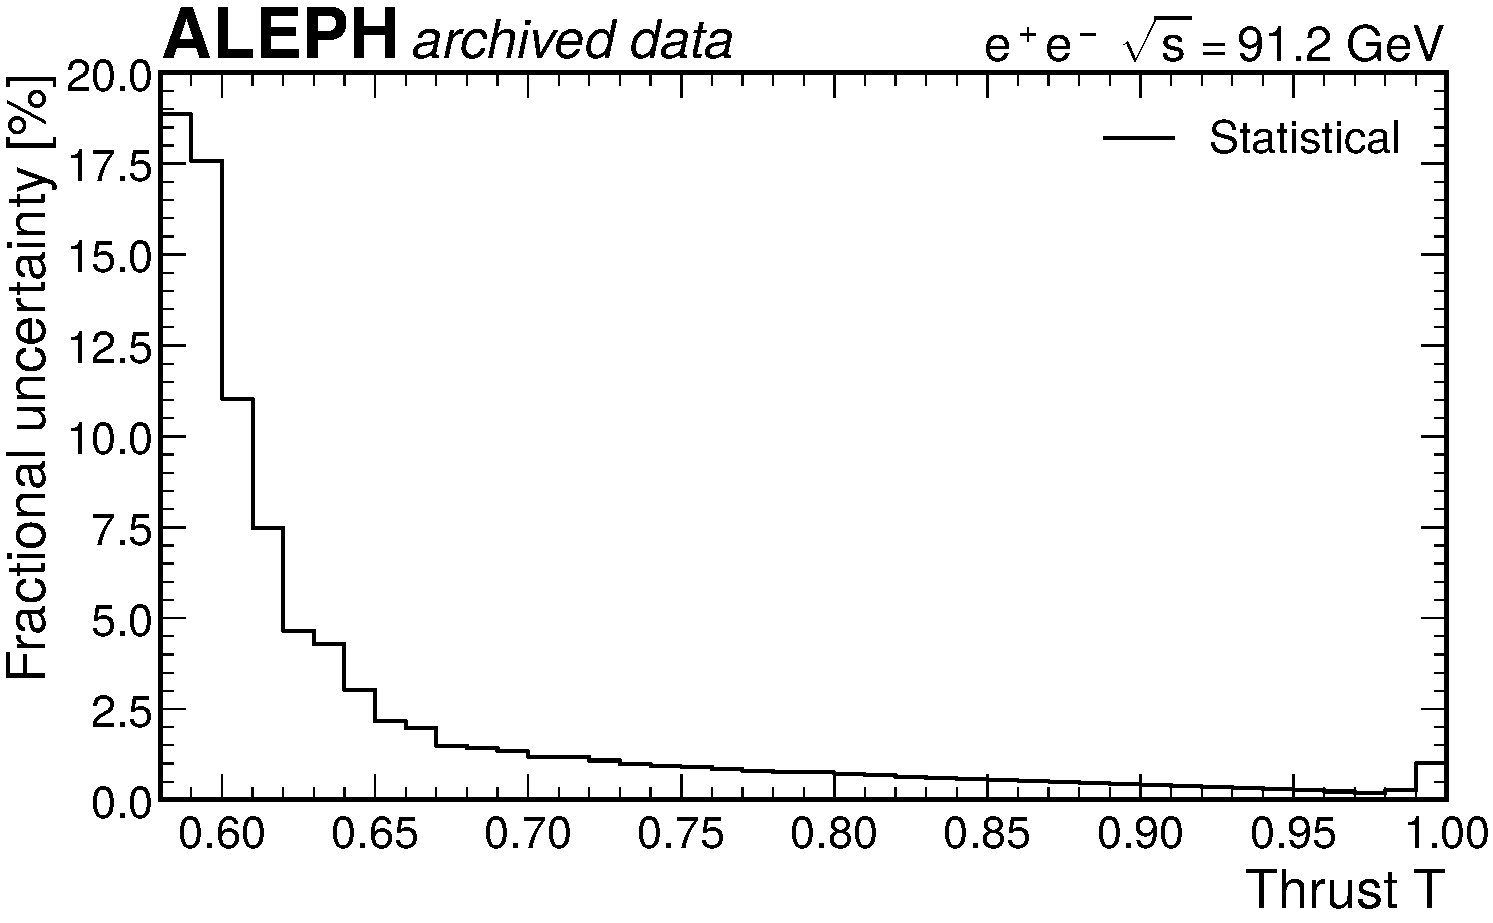
\includegraphics[width=0.49\textwidth]{figures/uncertainty_components_statistical.pdf}%
\hfill%
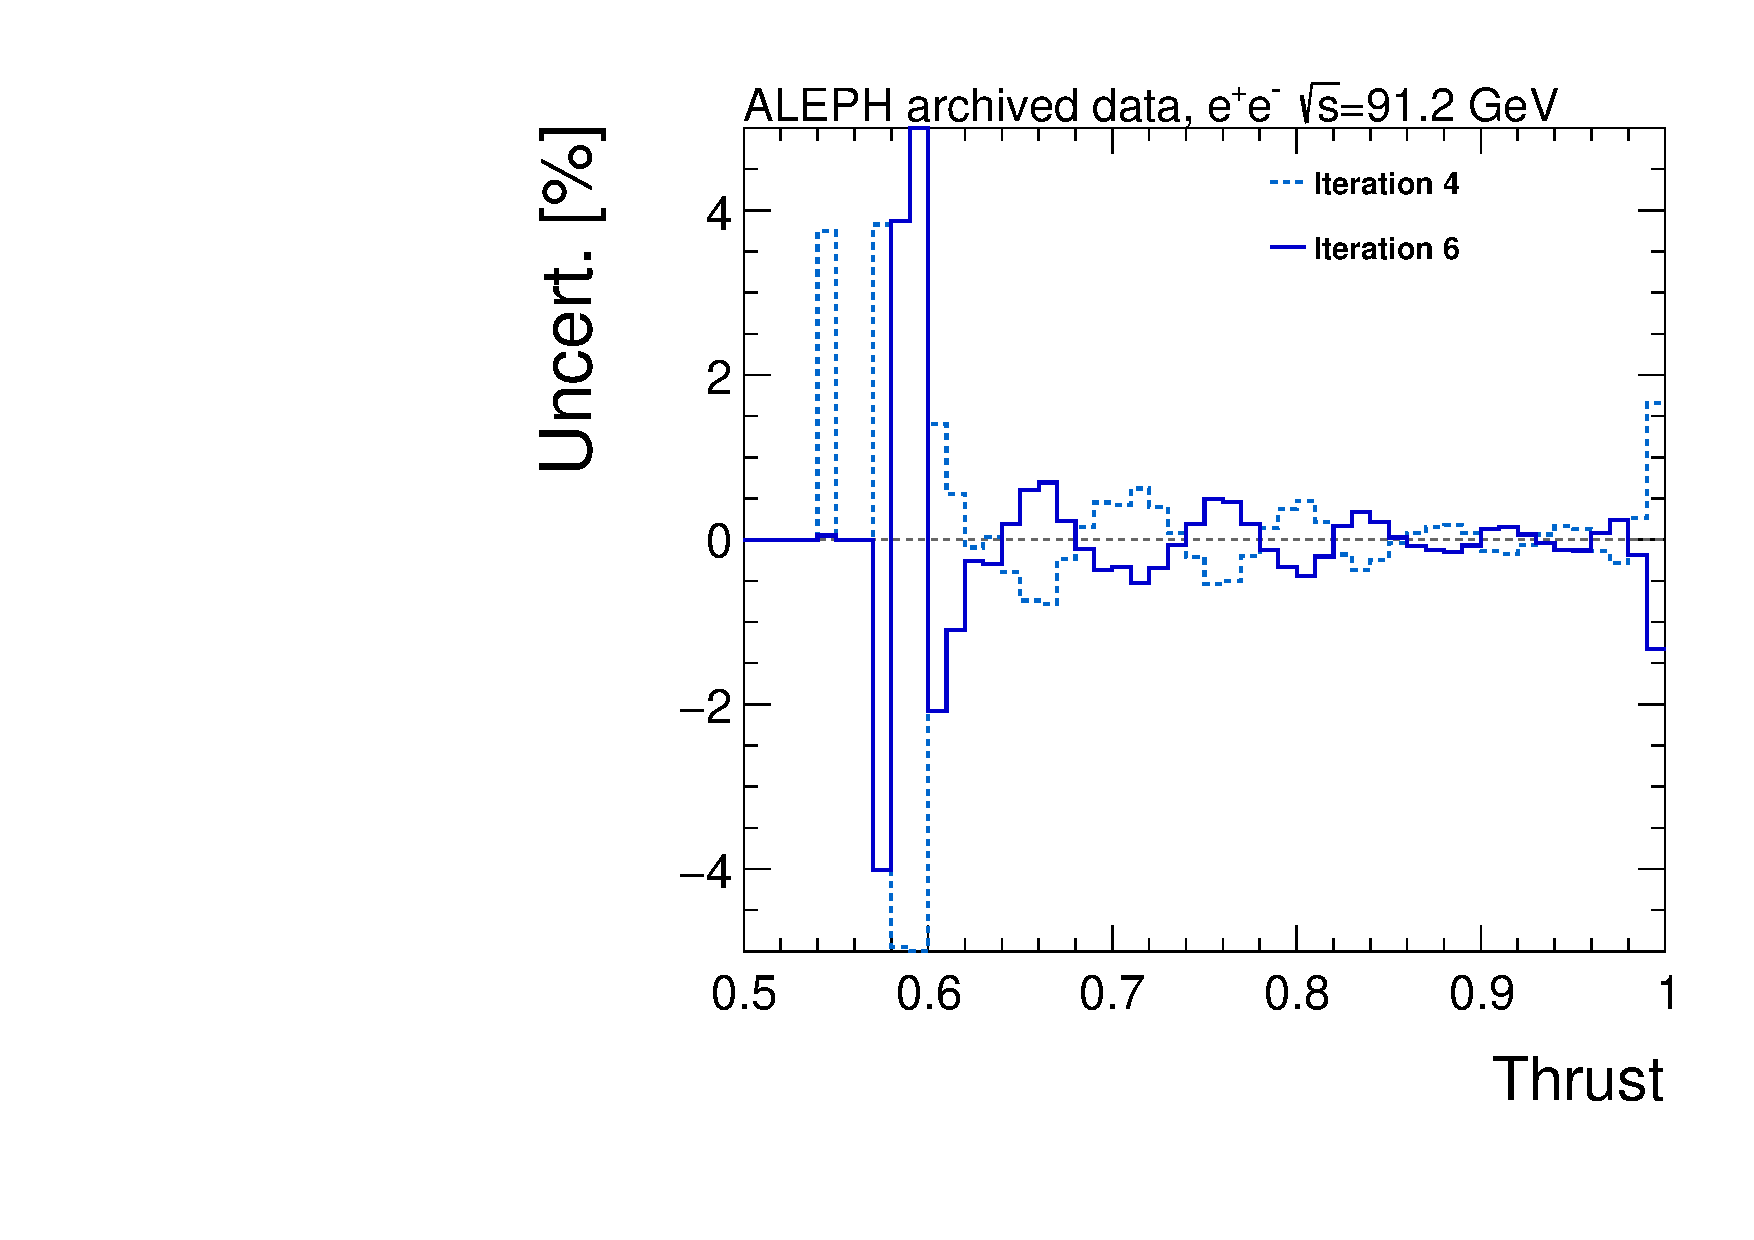
\includegraphics[width=0.49\textwidth]{figures/uncertainty_components_unfolding.pdf}
\caption{Signed per-bin shifts for the statistical (left) and unfolding-iteration
(right) uncertainty components. The statistical component is nearly flat and small
across the spectrum. The iteration panel shows $N_{\mathrm{iter}}=4$ and $6$
relative to the nominal $N_{\mathrm{iter}}=5$.}
\label{fig:unc_comp_stat_iter}
\end{figure}

\FloatBarrier

\subsection{Experimental systematic uncertainties}
\label{sec:exp_systematics}

Experimental systematic uncertainties are handled following the standard ALEPH procedure~\cite{Heister:2003aj} to vary individual selections, rerunning the full analysis chain, and measuring the difference with respect to the nominal as the uncertainty. The systems are defined below. The experimental subtotal and the final total are formed by quadrature of their sub-components.

\begin{itemize}
  \item \texttt{iter4}/\texttt{iter6}: unfolding passes at $N_{\mathrm{iter}}=4$ and $6$.
  \item \texttt{ntpc7}: tightened TPC hit requirement ($N_{\mathrm{TPC}}>7$, nominal $>4$).
  \item \texttt{pt04}: raised charged-$p_T$ threshold ($>0.4$~GeV, nominal $>0.2$~GeV).
  \item \texttt{ech10}: loosened charged-energy cut ($>10$~GeV, nominal $>15$~GeV).
  \item \texttt{with\_met}: missing transverse energy added as a pseudo-particle.
  \item \texttt{nes\_up}/\texttt{nes\_down}: neutral energies scaled up and down, probing ECAL energy-scale uncertainty.
  \item \texttt{ner}: neutral objects randomly removed, probing reconstruction efficiency.
\end{itemize}

Figure~\ref{fig:unc_comp_exp} shows the signed per-bin shifts for all variations. The largest contributions arise at low thrust ($T\lesssim 0.62$) where the steeply rising spectrum amplifies small absolute shifts; across the central range the experimental envelope is at the few-percent level.

\begin{figure}[ht!]
\centering
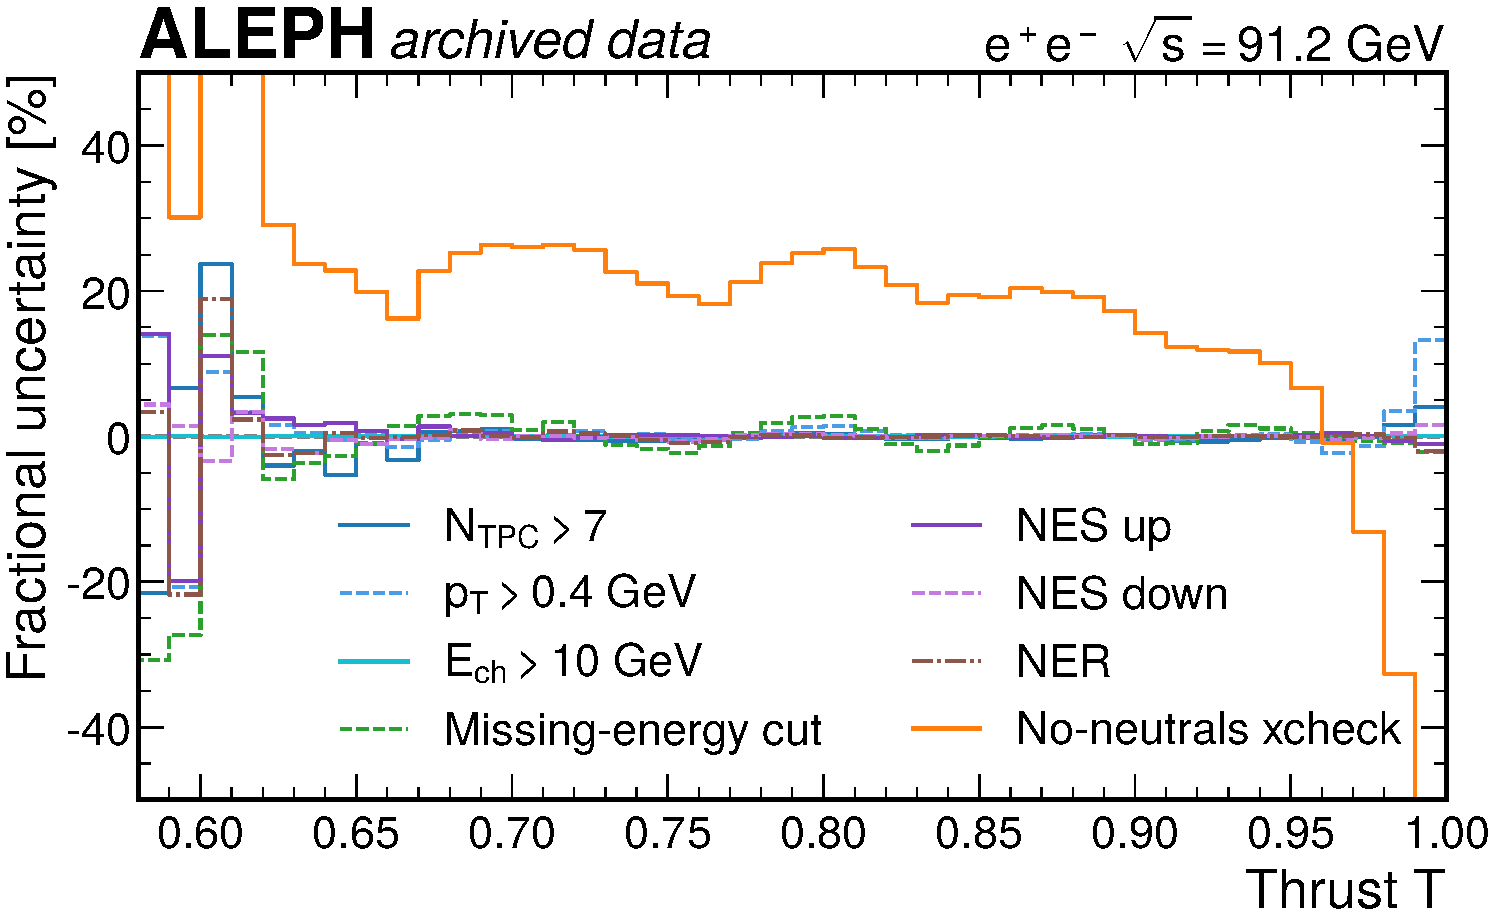
\includegraphics[width=0.85\textwidth]{figures/uncertainty_components_experimental.pdf}
\caption{Signed per-bin shifts for the seven experimental variation branches: the four
track/event branches (\texttt{ntpc7}, \texttt{pt04}, \texttt{ech10},
\texttt{with\_met}) and the three neutral-response branches (\texttt{nes\_up},
\texttt{nes\_down}, \texttt{ner}). The \texttt{no\_neutrals} curve is a cross-check and
does not enter the uncertainty.}
\label{fig:unc_comp_exp}
\end{figure}

The neutral-object response variations are chosen in preference to the standard ALEPH approach of removing all neutral particles within 1-2 GeV from the event~\cite{Heister:2003aj}. The reason is that
removing neutrals entirely redefines the observable: the resulting distribution is no longer the energy-flow thrust $T_{\mathrm{EF}}$ but a different quantity, charged-only thrust $T_{\mathrm{ch}}$, computed from a different particle-level definition. Treating the difference $T_{\mathrm{EF}} - T_{\mathrm{ch}}$ as a systematic uncertainty on the energy-flow measurement would conflate two distinct observables and produce an uncertainty that is unphysically large. Instead, \texttt{nes\_up}, \texttt{nes\_down}, and \texttt{ner} vary the detector response to neutral objects while holding the particle-level definition fixed, providing a physically meaningful probe of calorimeter modeling uncertainties without changing
what is being measured.

To quantify this distinction, the full unfolding chain was repeated with neutral particles ($\mathrm{pwflag}\in\{4,5\}$) removed, yielding a charged-only thrust distribution as shown in Figure~\ref{fig:charged_vs_ef}. Both the energy-flow and charged-only results are processed through the complete analysis chain. The reconstructed particle collection differs between the two, but both are unfolded to the same energy-flow particle-level definition. Both distributions are shown with statistical uncertainties only; the full systematic suite is not propagated for this diagnostic comparison, and the charged-only branch is excluded from the nominal total uncertainty combination. The charged-only spectrum is systematically broader than the energy-flow, as expected from the missing neutral-energy deposits. In the central range the mean shift is approximately $23\%$.

\begin{figure}[t!]
\centering
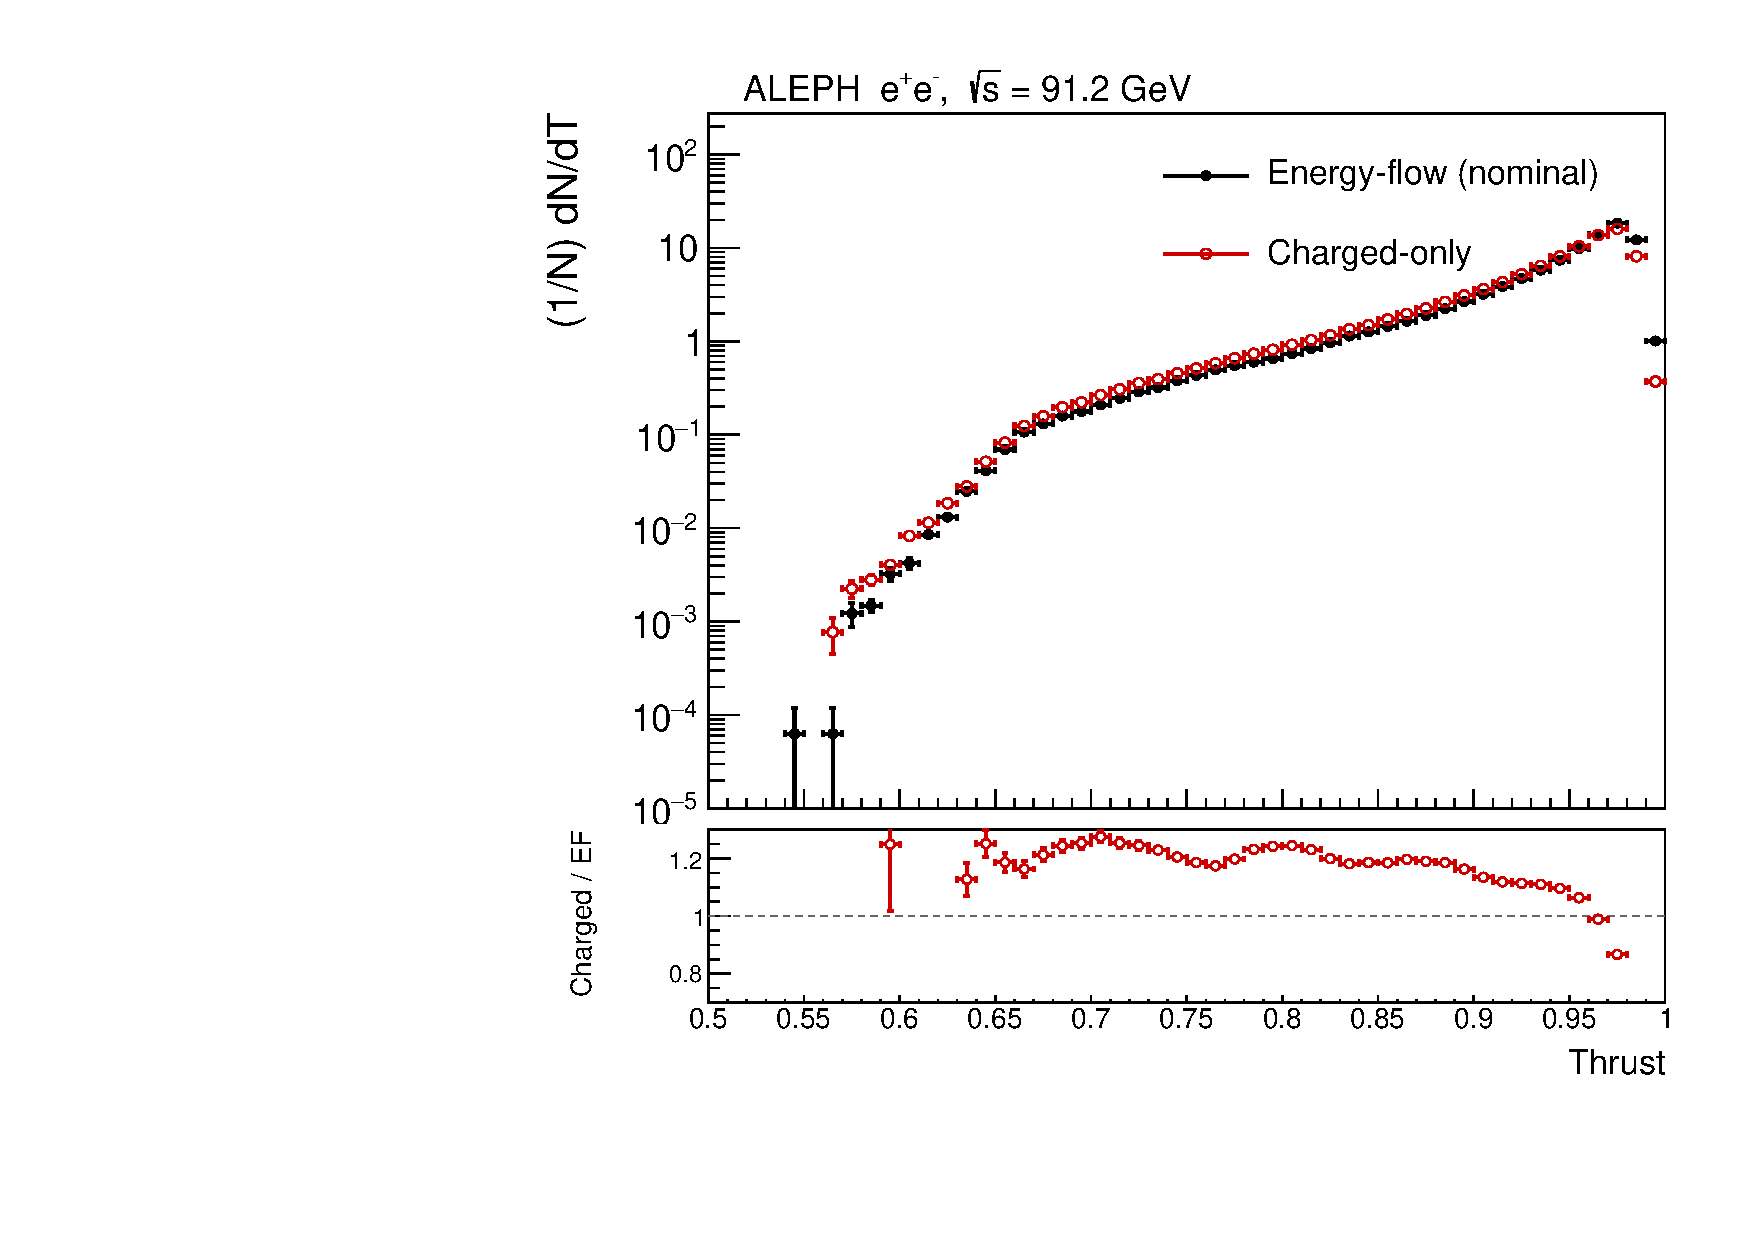
\includegraphics[width=0.70\textwidth]{figures/charged_only_vs_energy_flow.pdf}
\caption{Comparison of the charged-only (red open circles) and energy-flow (black filled circles) unfolded thrust distributions. Error bars represent statistical uncertainties only.}
\label{fig:charged_vs_ef}
\end{figure}

The track and neutral object variations are combined as described below. The full experimental envelope is then combined in quadrature.

\begin{align}
\Delta_{\mathrm{track/event}}(j) &=
  \sqrt{\sum_{v\in\{\mathrm{ntpc7,\,pt04,\,ech10,\,with\_met}\}} |\delta_v(j)|^2}. \\
  \Delta_{\mathrm{neutral}}(j) & =
\sqrt{\max\!\left(|\delta_{\mathrm{nes\_up}}(j)|,|\delta_{\mathrm{nes\_down}}(j)|\right)^2
    + |\delta_{\mathrm{ner}}(j)|^2}. \\ 
\Delta_{\mathrm{exp}}(j) &= \sqrt{\Delta_{\mathrm{track/event}}^2(j)+\Delta_{\mathrm{neutral}}^2(j)}.
\end{align}

\FloatBarrier

\subsection{Theory systematic uncertainties}
\label{sec:theory_systematics}

Theory systematic variations probe the residual model dependence introduced by the Monte Carlo generator used in the unfolding. The nominal response matrix is constructed from \textsc{Pythia}~6~\cite{Sjostrand:2000wi}, the ALEPH simulation. Three additional generators are used to reweight the generator-level thrust distribution event-by-event, producing alternative response matrices that span a
wide range of parton-shower algorithms and hadronization models: \textsc{Pythia}~8.317 with Monash tune, dipole-ordered shower~\cite{Bierlich:2022pfr}, \textsc{Herwig}~7.1.5, angular-ordered shower with cluster hadronization~\cite{B_hr_2008,Bellm:2015jjp,Bellm:2017bvx, bewick2024herwig73releasenote}, and \textsc{Sherpa}~2.2.6 with AHADIC++ hadronization~\cite{Bothmann2019}.
The theory envelope is taken as the maximum absolute shift across the three generators:
\begin{equation}
\Delta_{\mathrm{theory}}(j)=
  \max\!\left(|\delta_{\mathrm{pythia8}}(j)|,
             |\delta_{\mathrm{herwig}}(j)|,
             |\delta_{\mathrm{sherpa}}(j)|\right).
\end{equation}
The three generators diverge progressively at lower thrust, where multi-jet configurations and hard, wide-angle gluon emission dominate and the parton-shower and matrix-element matching differ between generators; there the reweighted
generator-level spectra move coherently and by similar amounts. The envelope also rises in the last bin, $0.99\le T<1.00$, where the reweighted spectra are least well constrained: the bin sits at the edge of the two-jet limit, and the shift there is not smoothly connected to its neighbours. The theory envelope is the dominant uncertainty contribution across the central measurement range, as shown in Figure~\ref{fig:unc_comp_theory}.

\begin{figure}[ht!]
\centering
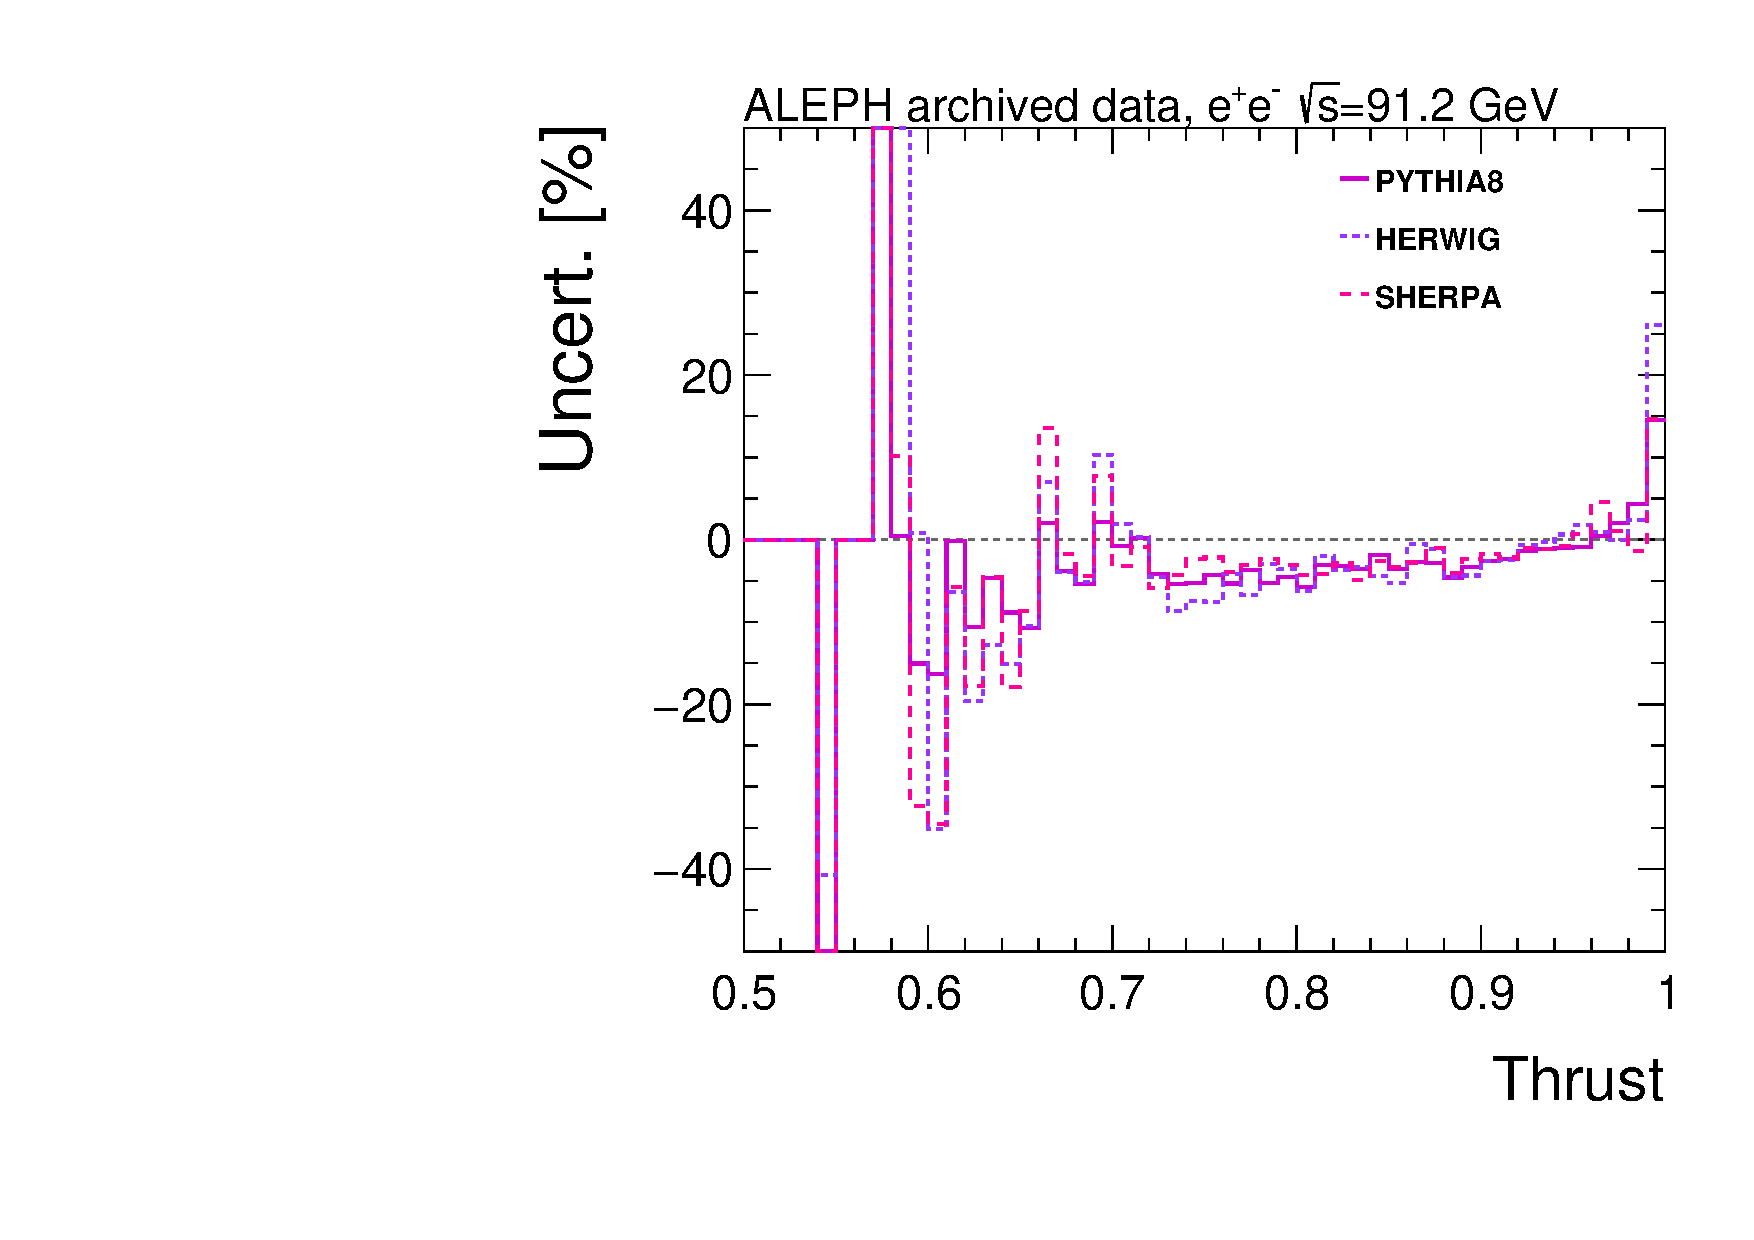
\includegraphics[width=0.85\textwidth]{figures/uncertainty_components_theory.pdf}
\caption{Signed per-bin shifts for the theory prior variations from \textsc{Pythia}~8.317, \textsc{Herwig}~7.1.5, and \textsc{Sherpa}~2.2.6.}
\label{fig:unc_comp_theory}
\end{figure}

\FloatBarrier

\subsection{Hadronic event-selection correction}
\label{sec:had_uncertainty}

After unfolding, a bin-wise hadronic event-selection correction is applied to account for the fraction of hadronic events lost to the generator-level selection:
\begin{equation}
C_{\mathrm{had}}(j) = \frac{N_{\mathrm{genBefore}}(j)}{N_{\mathrm{gen}}(j)},
\qquad
U_j^{\mathrm{corr}} = U_j\,C_{\mathrm{had}}(j).
\end{equation}
This correction maps the unfolded spectrum from the generator-level hadronic-event-selected phase space to the full inclusive hadronic phase space. The uncertainty on this correction is propagated as an independent component
$\Delta_{\mathrm{had}}$. The correction is computed from two generator-level histograms: \texttt{tgenBefore} (events before hadronic selection) and \texttt{tgen} (events passing hadronic selection). Statistical uncertainties on both histograms are propagated through the ratio using standard error propagation, yielding symmetric bin-wise up and down variations $C_{\mathrm{had}}^{\pm}(j)$. These variations are applied to the unfolded spectrum and normalized to the differential cross-section basis, producing up and down shifted spectra. 

% The fractional hadronic correction uncertainty is then defined as the envelope:
% \begin{equation}
% \delta_{\mathrm{had}}^{\pm}(j) = \frac{U_j \cdot C_{\mathrm{had}}^{\pm}(j) / \int U \cdot C_{\mathrm{had}}^{\pm}\,dT}{U_j^{\mathrm{corr}}} - 1,
% \end{equation}
% with $\Delta_{\mathrm{had}}(j) = \max(|\delta_{\mathrm{had}}^{+}(j)|, |\delta_{\mathrm{had}}^{-}(j)|)$.

\subsection{QED ISR correction}
\label{sec:isr_uncertainty}

The QED ISR correction removes the contribution of events
where the $e^+e^-$ center-of-mass energy is reduced by photon radiation before the hard scatter, mapping the measured distribution from the ISR-inclusive sample
to the pure $\sqrt{s}=M_Z$ distribution:
\begin{equation}
C_{\mathrm{ISR}}(j) = \frac{N^{\mathrm{gen}}_{\mathrm{no\,ISR}}(j)}{N^{\mathrm{gen}}_{\mathrm{ISR}}(j)}.
\end{equation}
Both published ALEPH event-shape analyses apply this
correction~\cite{Barate:1996fi,Heister:2003aj}. The 1998 ALEPH analysis~\cite{Barate:1996fi} defines it as the ratio of generator-level thrust distributions produced with and without ISR, using \textsc{JETSET}~7.4. The 2004 analysis~\cite{Heister:2003aj} uses \textsc{KORALZ}, which provides a more accurate treatment of ISR, to generate the corrected distribution.

The ISR correction is applied bin-by-bin after the hadronic correction using standalone \textsc{Pythia}~8.317 samples with ISR disabled (\texttt{isr0}) and enabled (\texttt{isr1}), as described in Sec.~\ref{sec:corrections_and_cov}. The uncertainty on
this correction is derived from the finite Monte Carlo statistics. Up and down variations $C_{\mathrm{ISR}}^{\pm}(j) = C_{\mathrm{ISR}}(j)\cdot(1\pm\sigma_{\mathrm{rel}}(j))$ are applied to the unfolded spectrum and the envelope is taken as $\Delta_{\mathrm{ISR}}(j)$. The uncertainty is purely MC-statistical in nature for simplicity, but should be assessed in closer detail for future work. 

% The \textsc{Pythia}~8.317 generator used here gives a less accurate ISR description than the \textsc{KORALZ} generator used in the ALEPH 2004 analysis~\cite{Heister:2003aj}; for a full measurement the modern equivalent, \textsc{KKMCee}~5.00.02, would be the natural choice, as noted in Sec.~\ref{sec:corrections_and_cov}.

\subsection{Covariance evaluation}
\label{sec:stat_covariance}

For the nominal run, the statistical covariance is computed by RooUnfold using analytical error propagation (\texttt{RooUnfold::kCovariance}), which propagates
Poisson uncertainties in the data and response histograms through the IBU iteration chain without toy MC sampling. The resulting covariance matrix is read from the unfolding output and transformed to the normalized differential-thrust basis used in this work.

Non-statistical component covariances are built with a configurable model. The current nominal release uses the \texttt{template\_correlated} option, where each non-statistical component covariance is built as
\begin{equation}
\mathrm{Cov}^{(c)}_{ij}=\Delta_c(i)\,\Delta_c(j)\,\rho^{\mathrm{stat}}_{ij},
\end{equation}
with $\rho^{\mathrm{stat}}_{ij}$ taken from the statistical unfolding covariance correlation template. This keeps component magnitudes tied to the measured per-bin
shifts while avoiding a purely diagonal systematic-covariance approximation. For cross-check studies, \texttt{diagonal} and \texttt{block} component models
are also available~\cite{Adye:2011gm}.

\subsection{Combination model}
\label{sec:combination_model}

The total bin uncertainty combines all seven components in quadrature:
\begin{equation}
\Delta_{\mathrm{tot}}(j)=\sqrt{\Delta_{\mathrm{stat}}^2(j)
+ \Delta_{\mathrm{iter}}^2(j) + \Delta_{\mathrm{exp}}^2(j)
+ \Delta_{\mathrm{theory}}^2(j) + \Delta_{\mathrm{had}}^2(j)
+ \Delta_{\mathrm{ISR}}^2(j)}.
\end{equation}
The quadrature sum is used since the components originate from distinct sources and the covariance cross terms are expected to be small.

\subsection{Uncertainty breakdown}
\label{sec:uncertainty_breakdown}

Figure~\ref{fig:per_bin_uncertainty_grid} shows the absolute fractional uncertainties. Theory is the dominant source across the central range, where the experimental envelope is smaller by roughly a factor of two. The statistical and iteration components remain sub-percent in the bulk.

\begin{figure}[ht!]
\centering
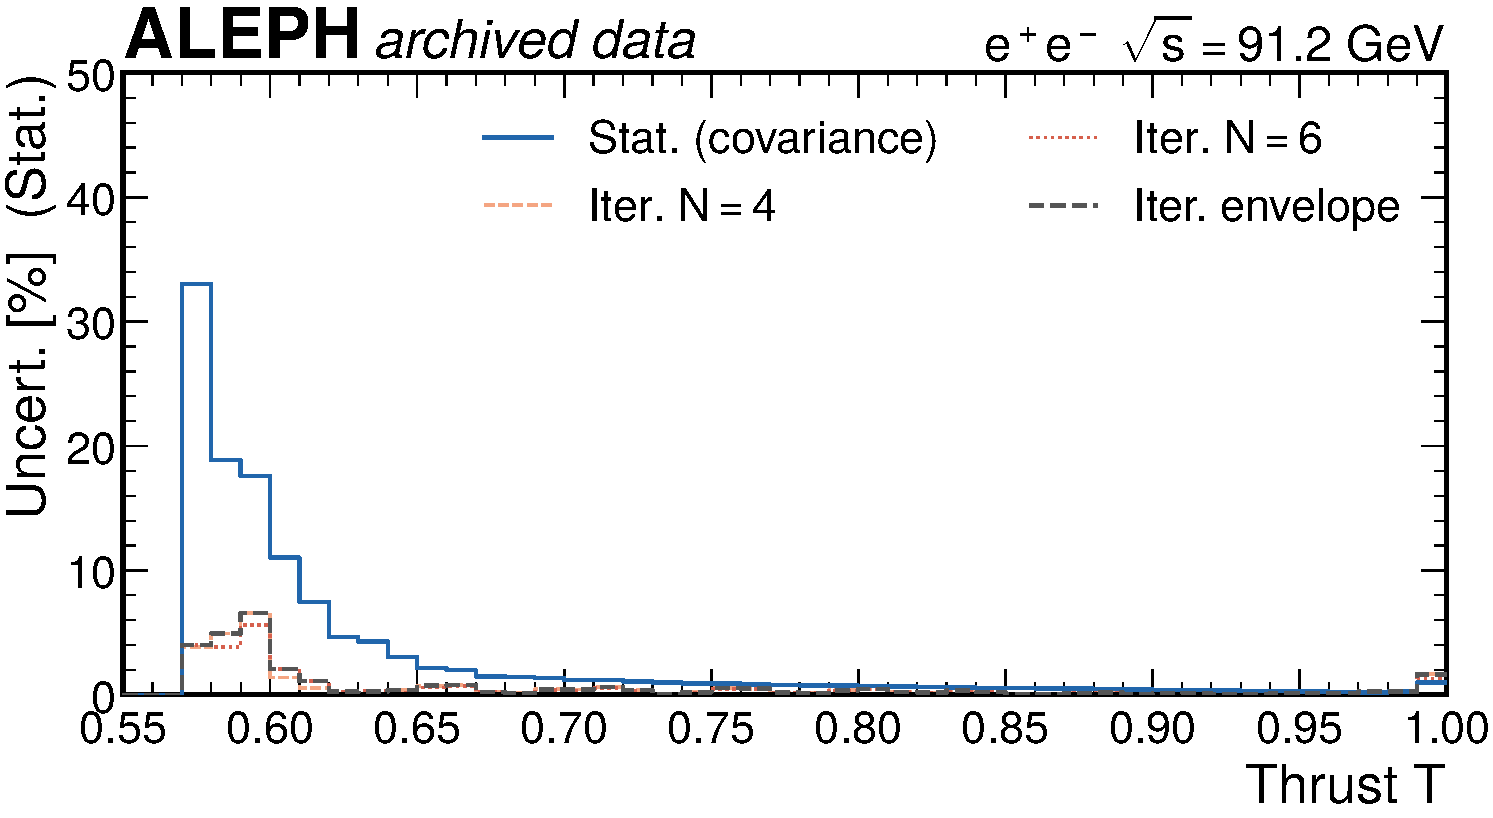
\includegraphics[width=0.49\textwidth]{figures/per_bin_uncertainty_stat.pdf}%
\hfill%
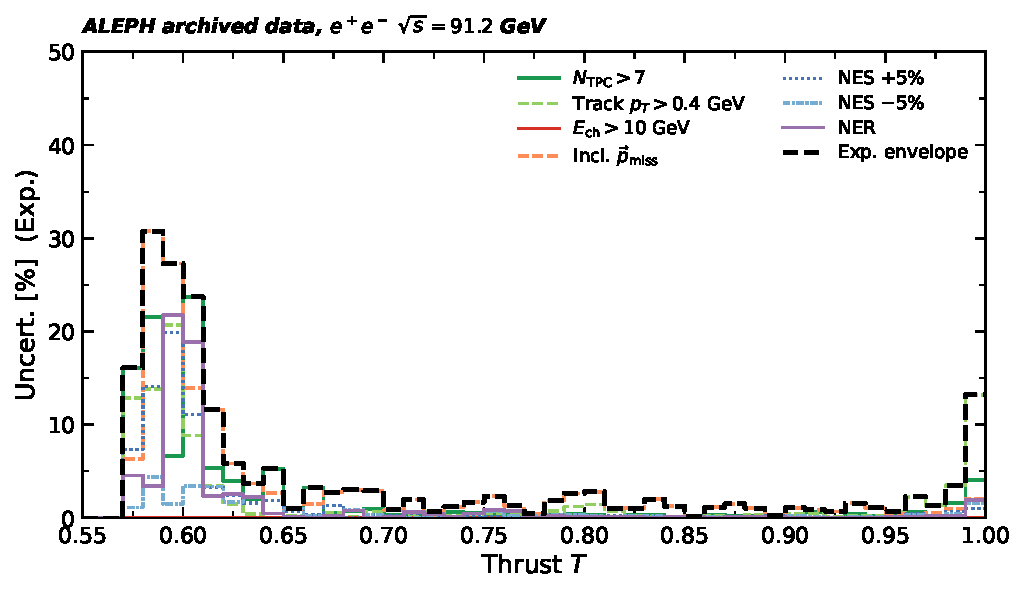
\includegraphics[width=0.49\textwidth]{figures/per_bin_uncertainty_exp.pdf}\\[2mm]
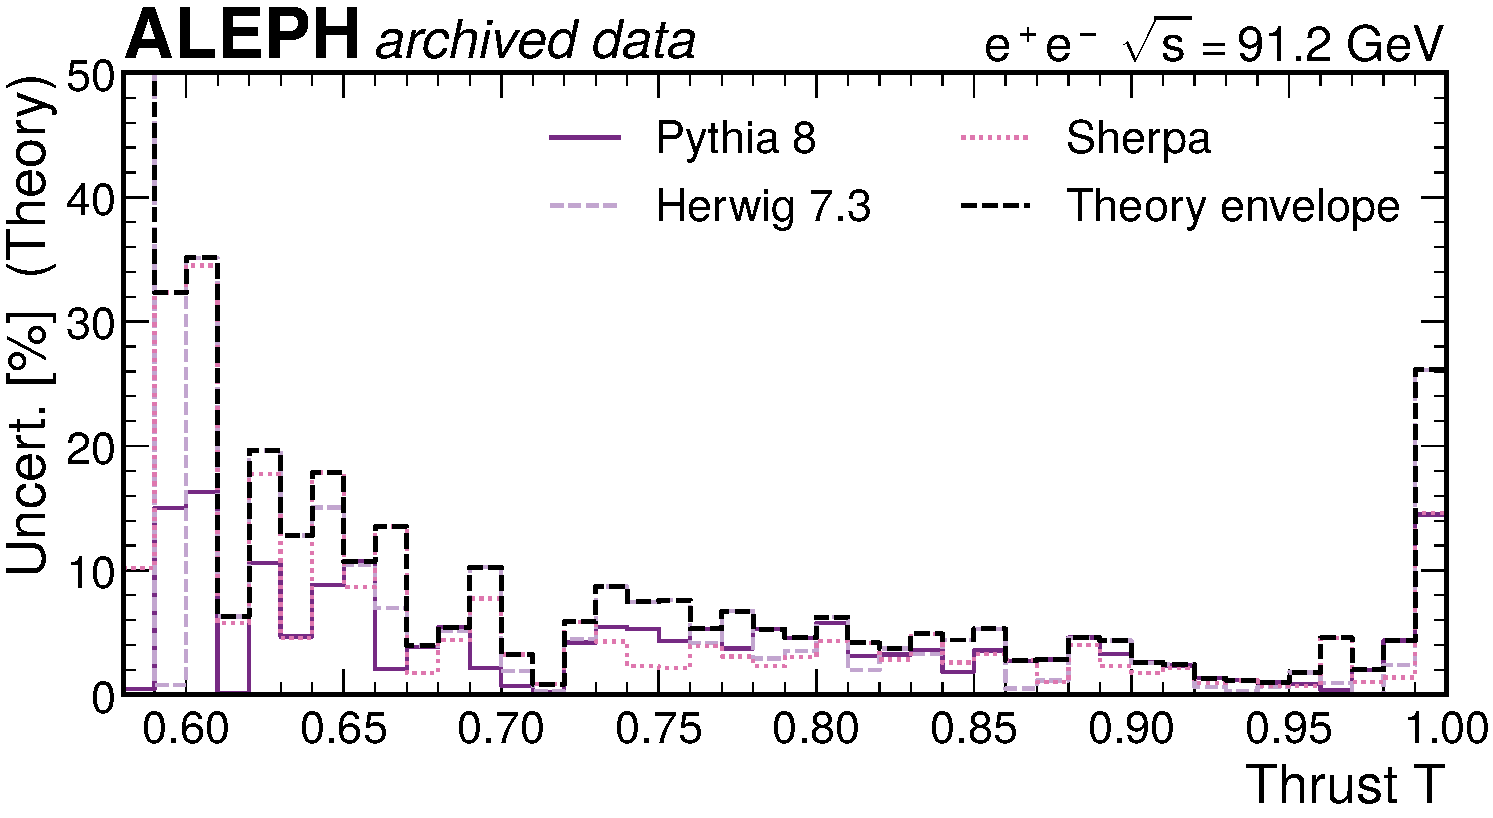
\includegraphics[width=0.49\textwidth]{figures/per_bin_uncertainty_theory.pdf}%
\hfill%
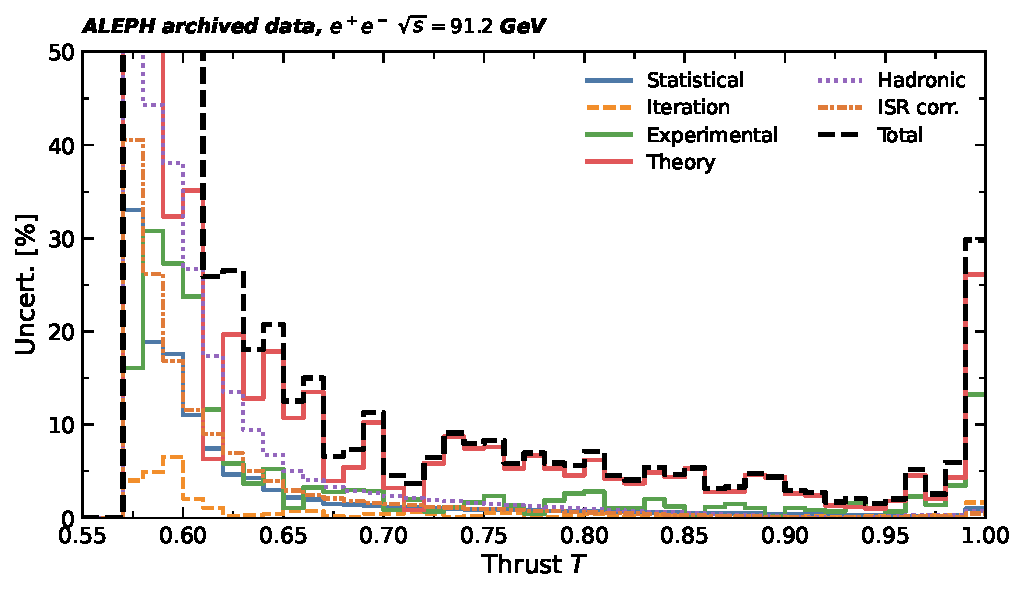
\includegraphics[width=0.49\textwidth]{figures/per_bin_uncertainty_grouped.pdf}
\caption{Fractional uncertainties: (top left) statistical and unfolding-iteration components, (top right) experimental variation branches with group envelope, (bottom left) theory reweighting branches with theory envelope, (bottom right) all groups overlaid.
%The neutral energy-scale branches respond non-linearly to a symmetric variation, so their up and down shifts differ at low thrust while agreeing across the reported range. The charged-$p_T$ branch peaks in the last bin, where removing soft tracks migrates events against the kinematic boundary.
}
\label{fig:per_bin_uncertainty_grid}
\end{figure}


\section{Results}
\label{sec:results}

The thrust baseline result is obtained from the 1994 workflow with Iterative Bayesian
Unfolding at nominal $N_{\mathrm{iter}}=5$, including the hadronic event correction,
ISR correction, and all configured systematic reruns.
All 14 nominal and systematic unfolding jobs completed successfully.
The response matrix diagonal fraction is 0.332, indicating substantial migration between
reconstructed and generated thrust bins.

\subsection{Final unfolded thrust distribution}

\begin{figure}[t!]
\centering
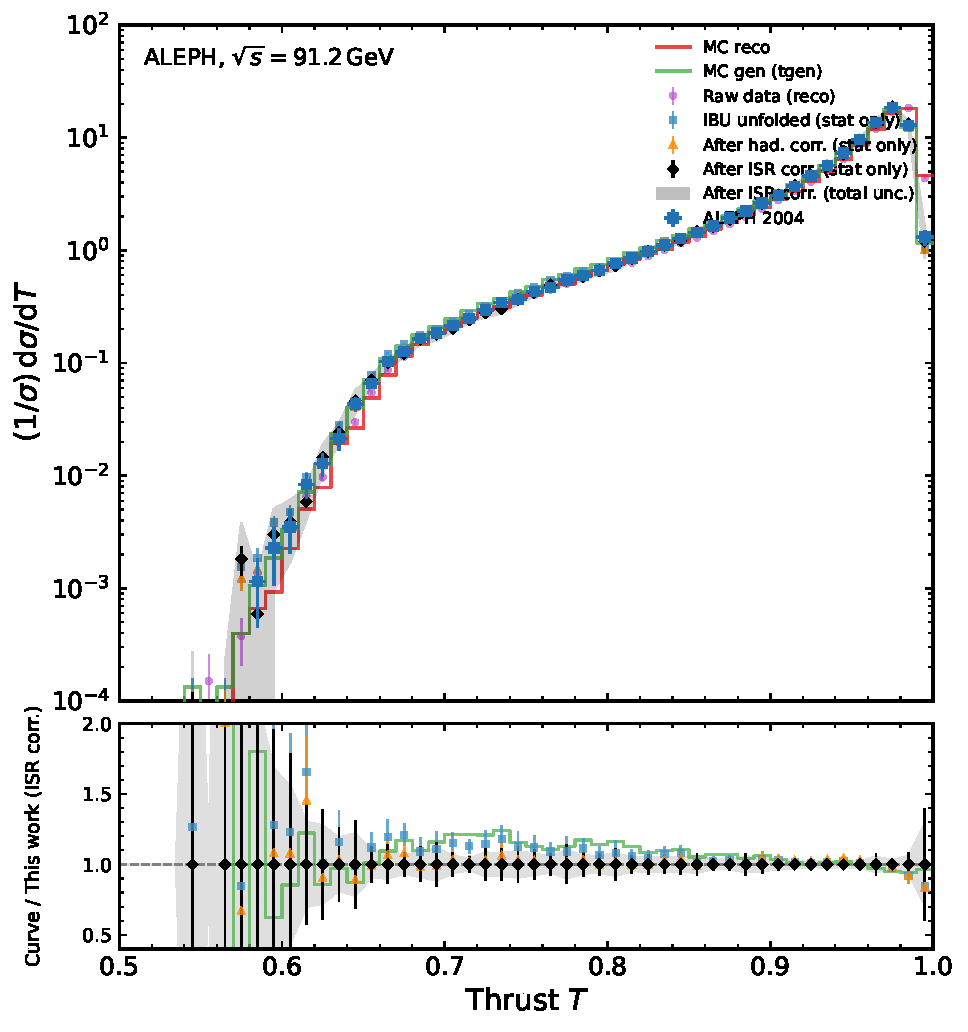
\includegraphics[width=0.49\textwidth]{figures/final_result_ratio_ours.pdf}%
\hfill%
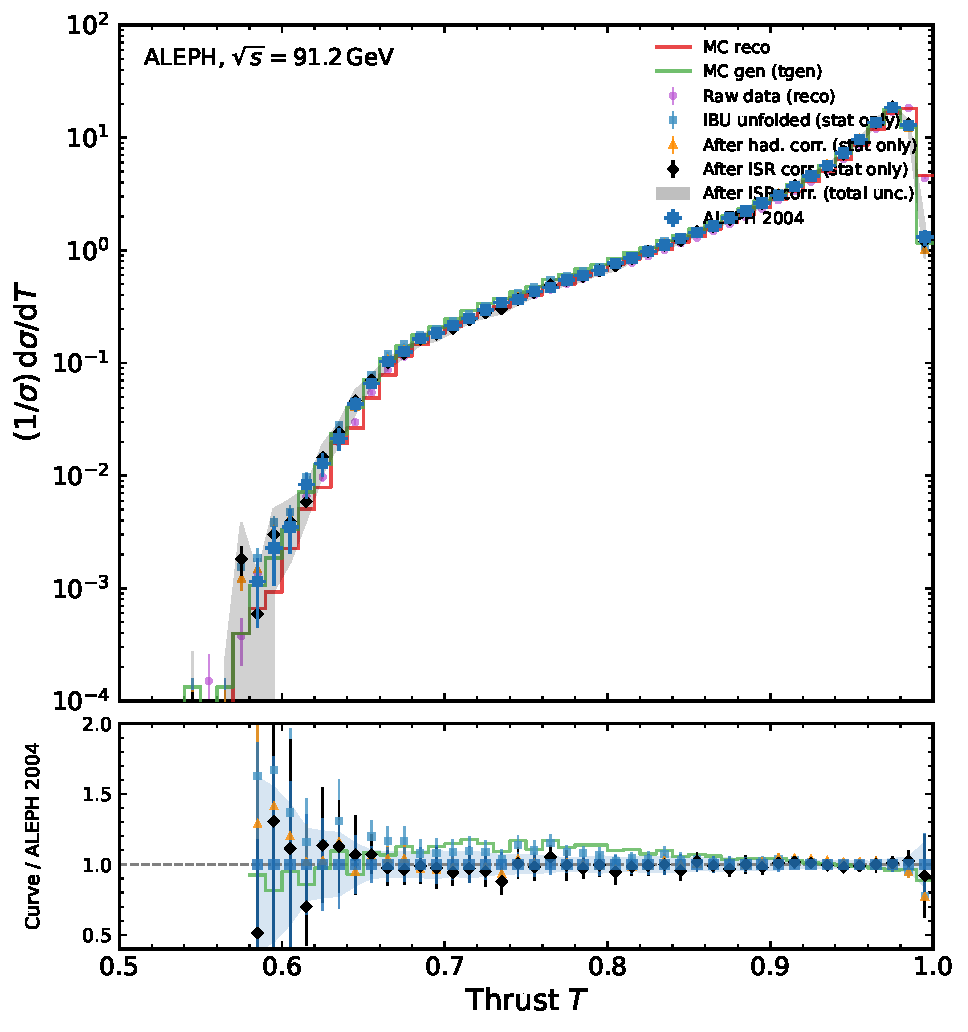
\includegraphics[width=0.49\textwidth]{figures/final_result_ratio_aleph.pdf}
\caption{Left: final unfolded thrust distribution showing all correction stages
(raw reco, MC reco, MC gen, IBU unfolded, after hadronic correction, after ISR correction)
compared to ALEPH 2004. The ratio panel is normalised to the fully corrected result of
this work; the gray band shows the total uncertainty envelope. Right: same stages with
the ratio panel normalised to the published ALEPH 2004 result. Agreement is good across
the bulk of the spectrum ($0.62\le T<0.99$); the elevated endpoint ratio ($1.30\pm0.27$)
is physically expected (soft-hadron sensitivity, hadronic/ISR correction growth,
normalisation convention differences).}
\label{fig:final_thrust_result}
\end{figure}

\begin{figure}[t!]
\centering
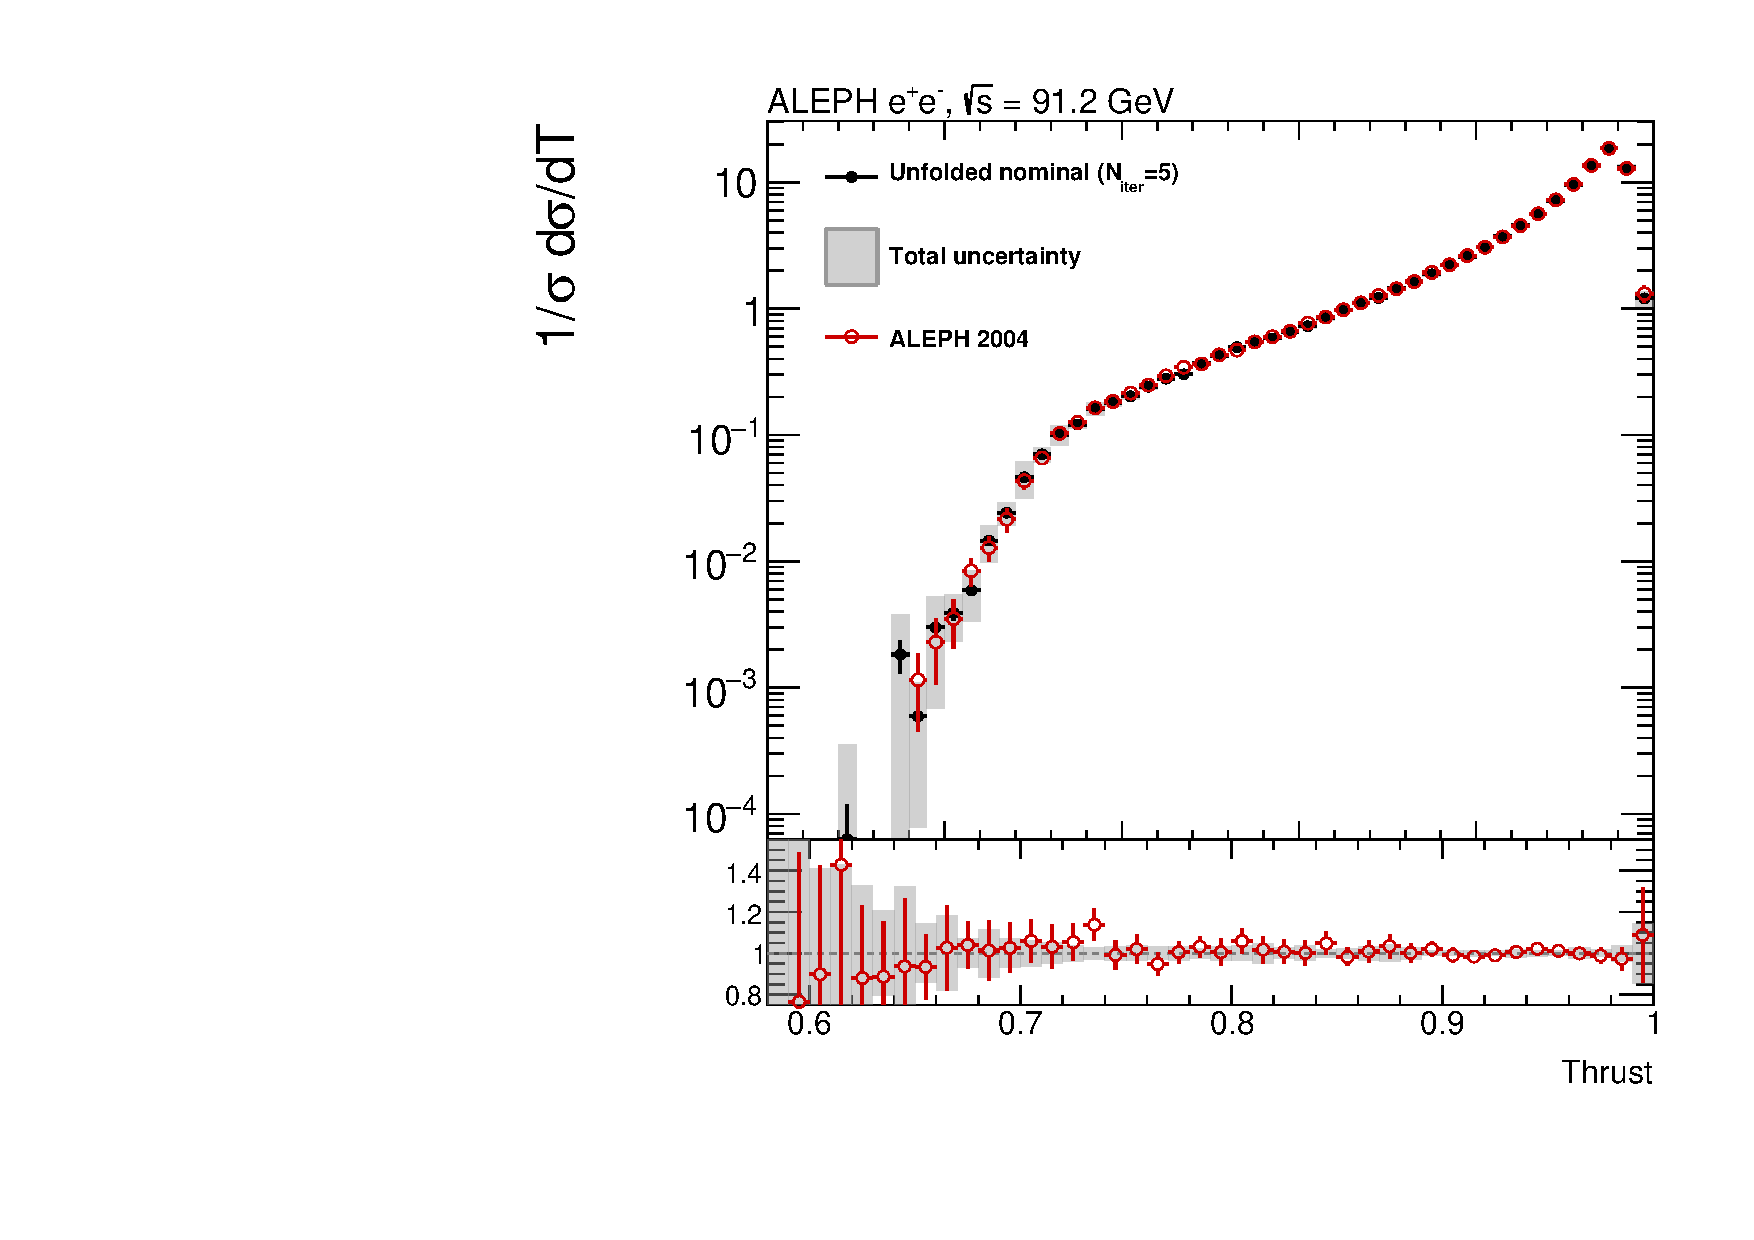
\includegraphics[width=0.48\textwidth]{figures/final_result_uncertainty_breakdown.pdf}%
\hfill%
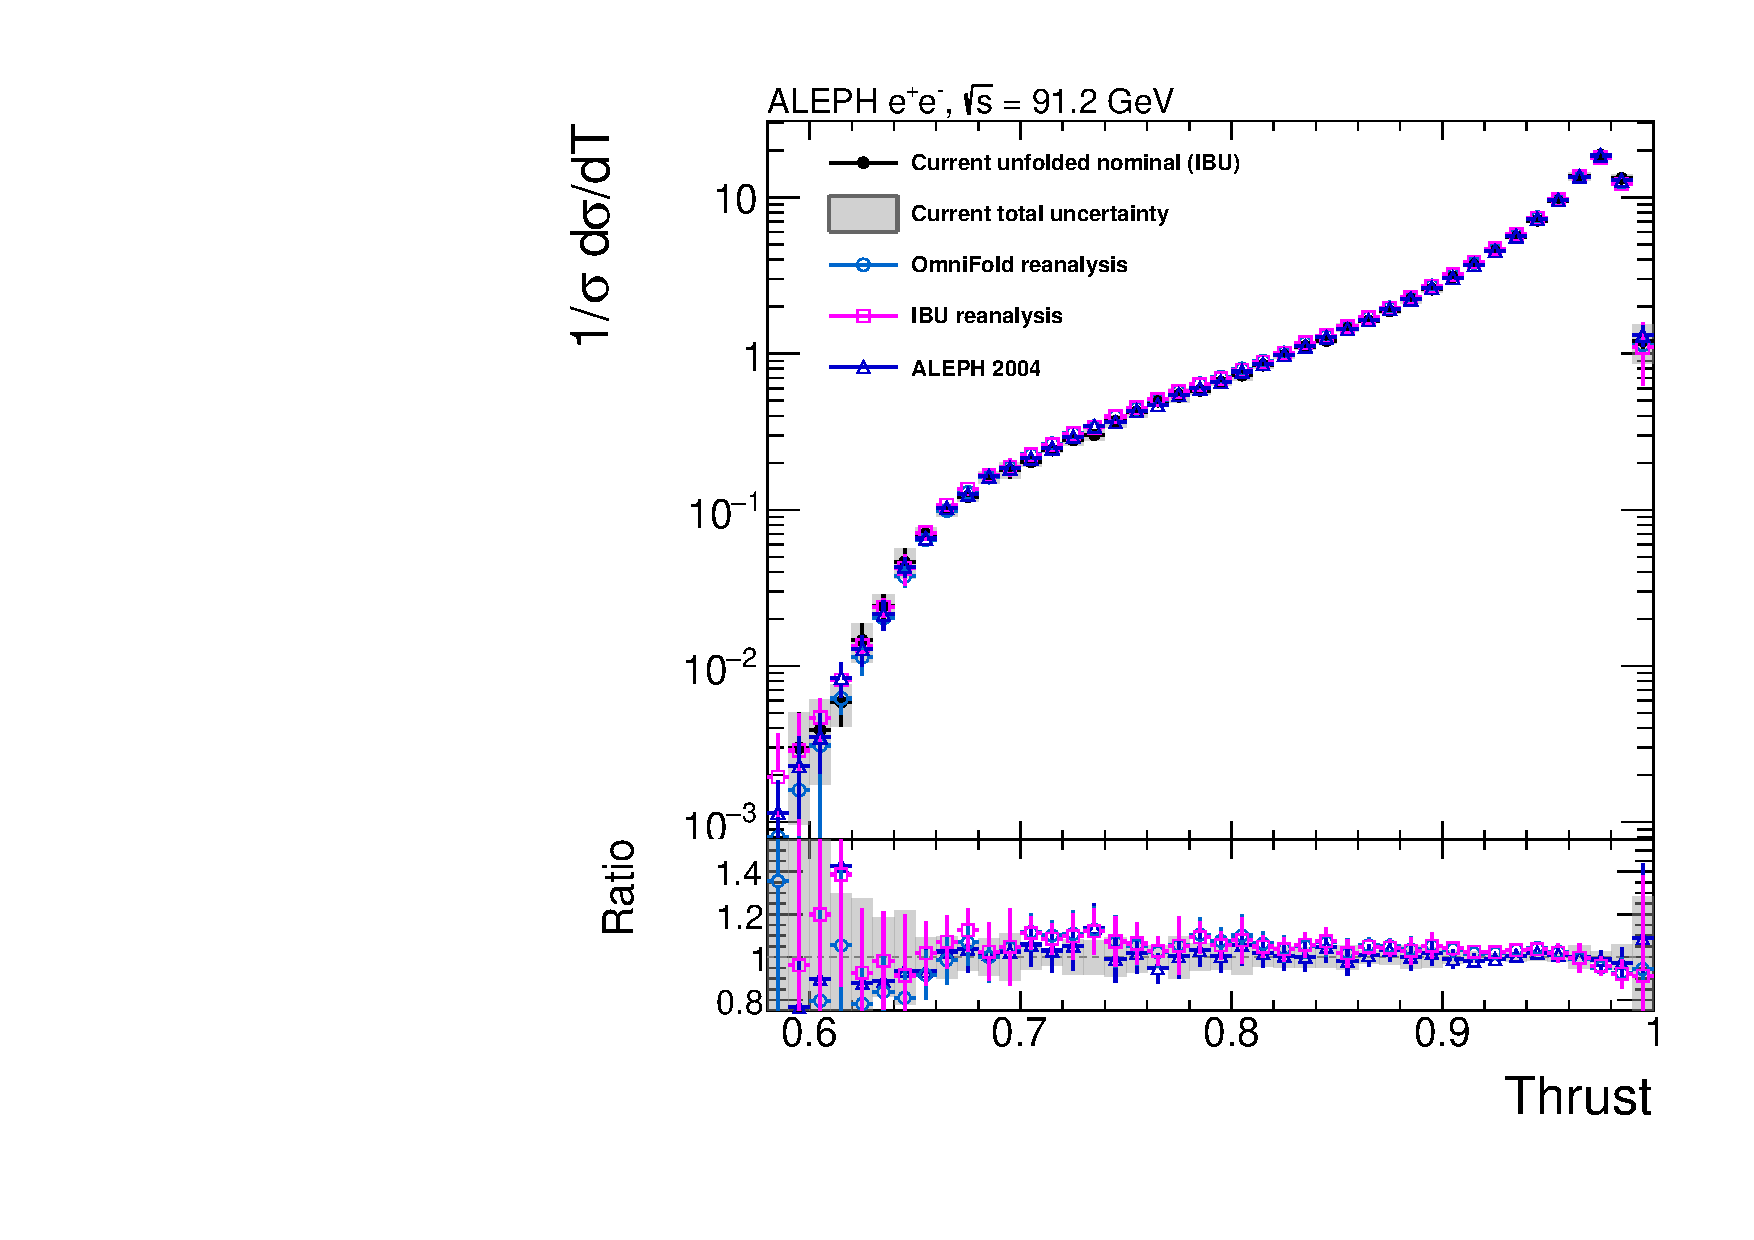
\includegraphics[width=0.48\textwidth]{figures/final_result_of_ibu_comparison.pdf}
\caption{Left: total uncertainty band for the final thrust result versus ALEPH 2004.
Right: comparison with OmniFold and prior IBU spectra; the ratio panel shows each
method relative to the current unfolded nominal. Compatibility metrics are
$\chi^2/\mathrm{ndf}=0.663$ (OmniFold), $0.421$ (prior IBU), and $0.361$ (ALEPH 2004),
evaluated over 42 bins using the diagonal of the total covariance.}
\label{fig:final_thrust_result_legacy}
\end{figure}

Figure~\ref{fig:final_thrust_result} (left) shows the unfolded spectrum with the total
uncertainty band and comparison to the published ALEPH 2004 result. Agreement is good
across the bulk of the spectrum ($0.62\le T<0.99$), with the largest discrepancy at
the endpoint ($0.99<T<1.00$, ratio $1.30\pm0.27$). This is physically expected: the
dijet limit is sensitive to MC modeling of soft hadrons, and the hadronic correction
$C_{\mathrm{had}}(j)$ and ISR correction $C_{\mathrm{ISR}}(j)$ carry growing
uncertainties there. Normalization convention differences between the current analysis
and the 2004 ALEPH publication also contribute at the endpoint.

Figure~\ref{fig:final_thrust_result} (right) shows direct comparison with OmniFold and
prior IBU spectra from the archived-data analysis program. Sub-unity $\chi^2/\mathrm{ndf}$
values reflect the conservative uncertainty model and positive off-diagonal correlations,
not overestimation. Differences are localized to the endpoint region.

\begin{figure}[t!]
\centering
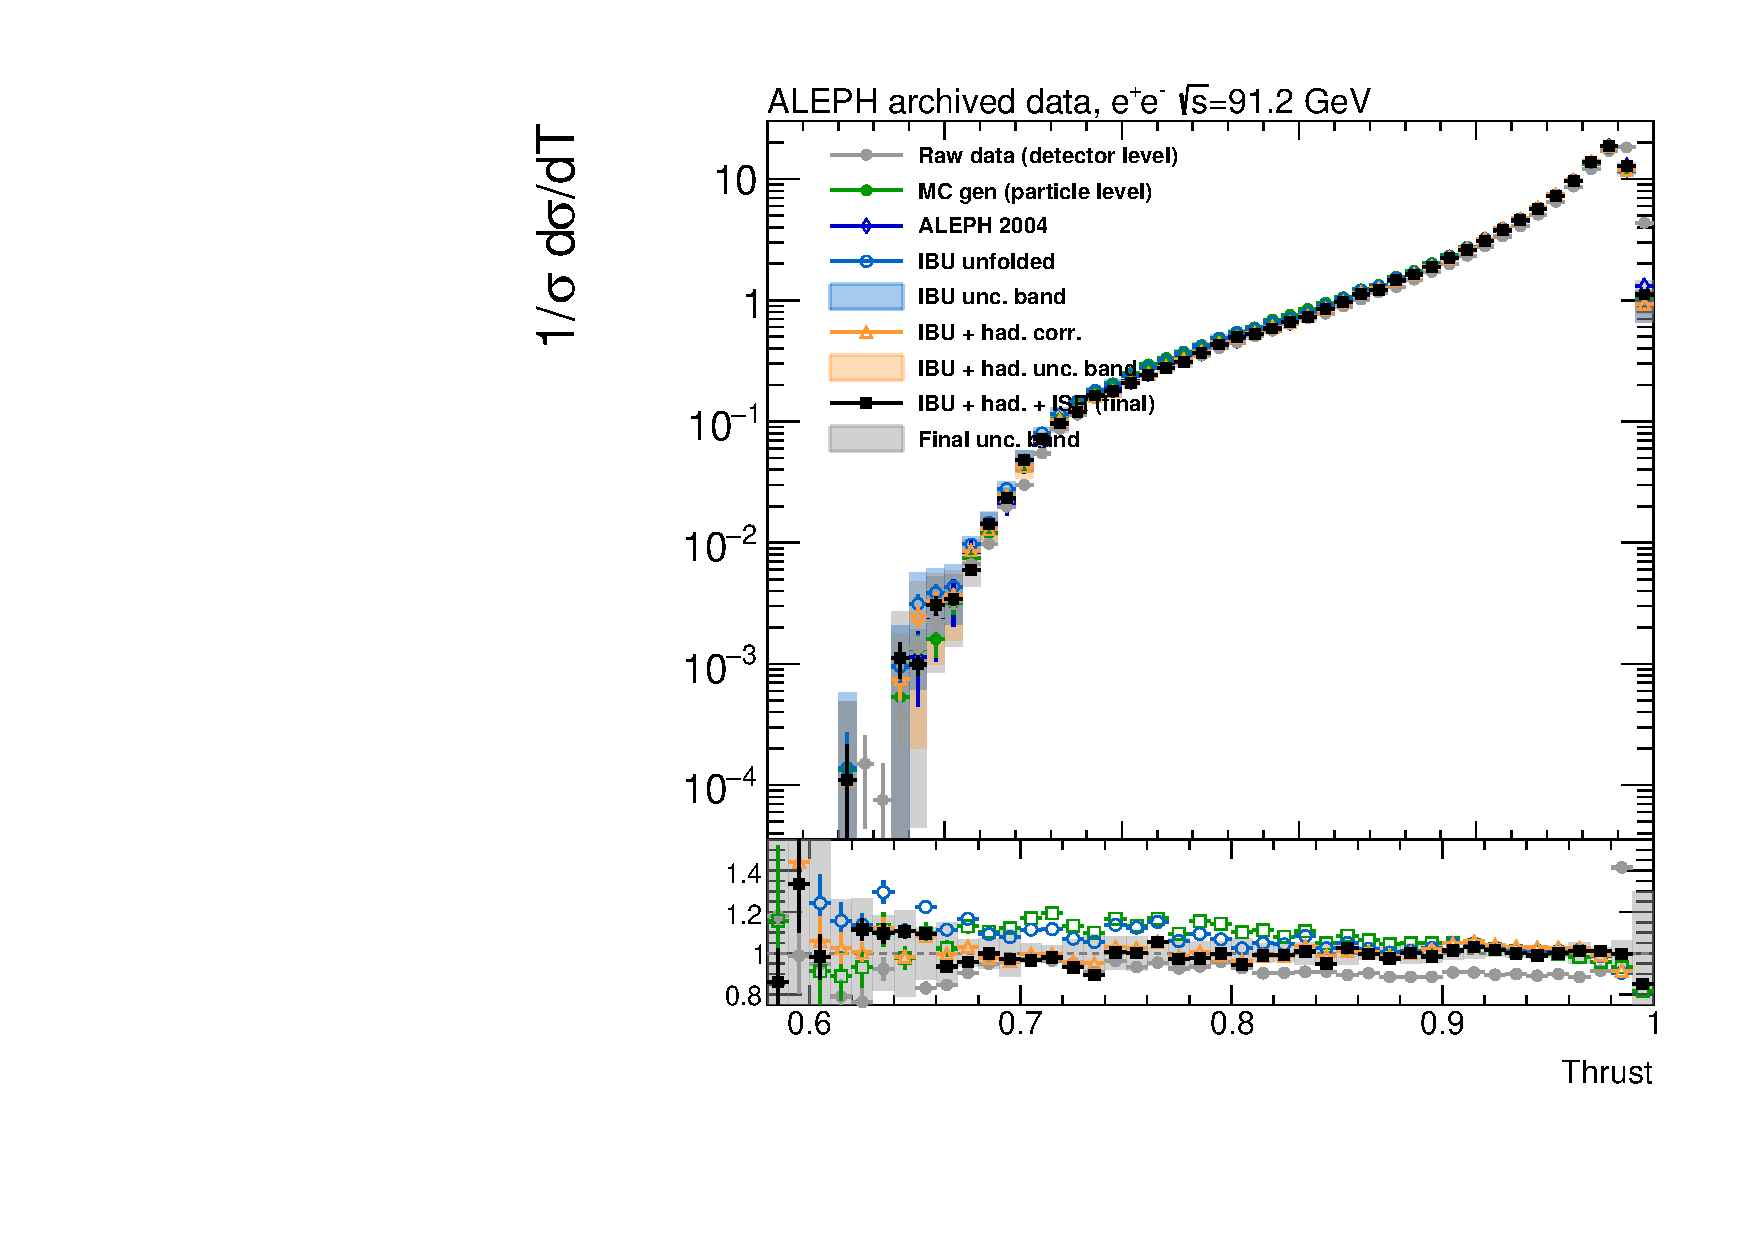
\includegraphics[width=0.49\textwidth]{figures/final_result_correction_stages.pdf}%
\hfill%
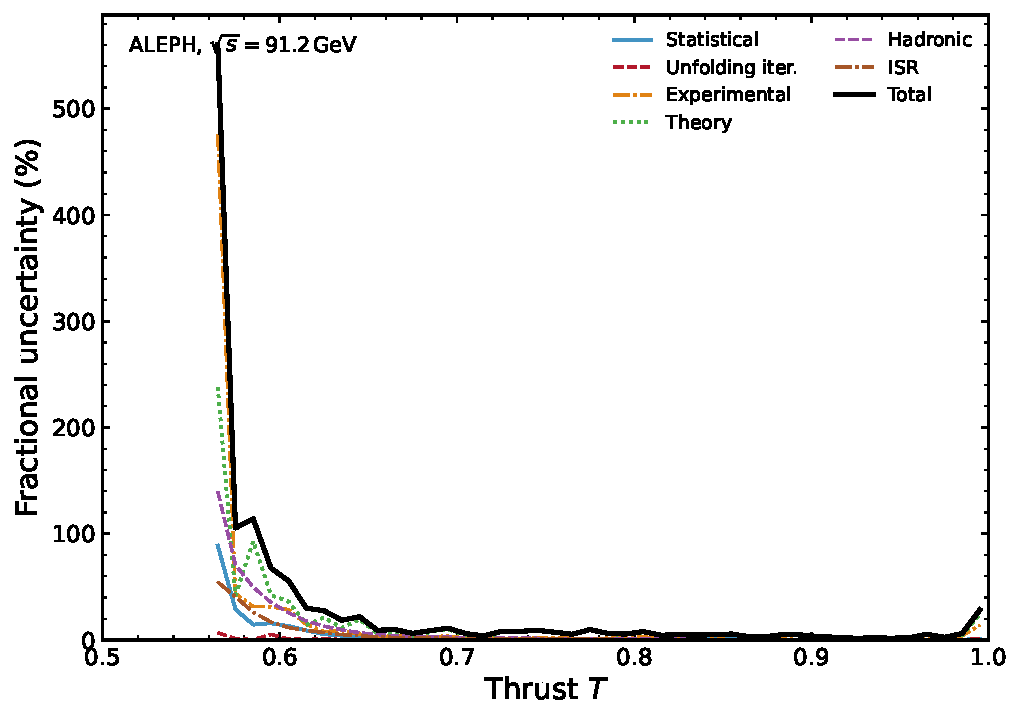
\includegraphics[width=0.49\textwidth]{figures/uncertainty_breakdown.pdf}
\caption{Left: all correction stages compared to ALEPH 2004, with ratio panel showing
each stage divided by the ALEPH 2004 result. The progression from IBU-only through
hadronic and ISR corrections is visible in the ratio panel. Right: fractional
per-component uncertainty as a function of thrust $T$. Theory dominates in the central
range; statistical and experimental components are sub-leading; ISR is small and nearly
flat.}
\label{fig:correction_stages_and_unc}
\end{figure}

The total correlation matrix for the combined result is shown in
Fig.~\ref{fig:final_total_correlation_matrix_sys}. The off-diagonal structure is
non-trivial and arises mainly from the unfolding of detector-level migration: it is
carried by the statistical (RooUnfold) covariance and by the systematic components that
inherit its correlation template. Under the nominal model the theory component enters as
a diagonal covariance (Sec.~\ref{sec:stat_covariance}) and therefore contributes only to
the per-bin variances, not to the bin-to-bin correlations. The off-diagonal correlations
remain non-negligible, so the full covariance matrix, rather than diagonal uncertainties
alone, must be used in any downstream fit or comparison.

\begin{figure}[t!]
\centering
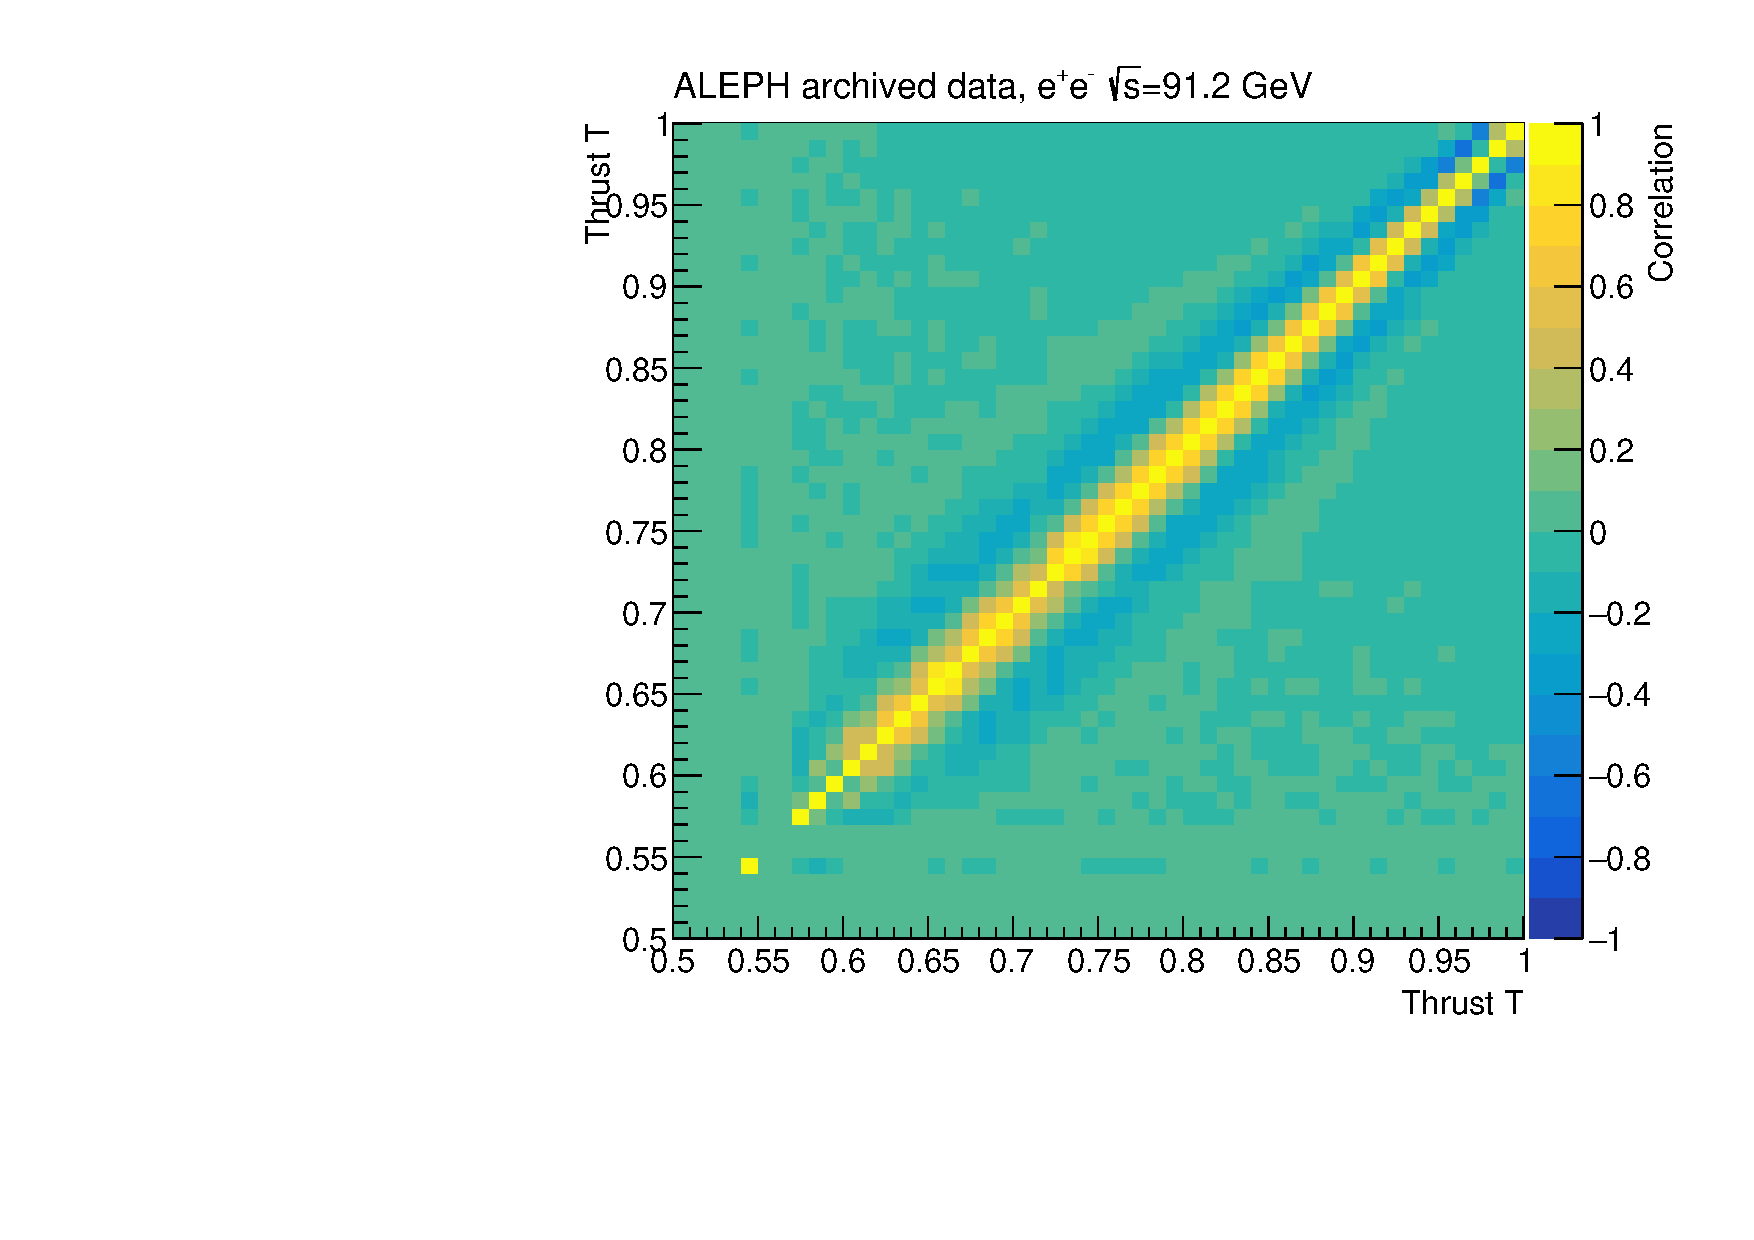
\includegraphics[width=\textwidth]{figures/matrix_total_correlation_final.pdf}
\caption{Total bin-to-bin correlation matrix for the final result, combining
statistical, unfolding-iteration, experimental, theory, hadronic-correction, and
ISR-correction components. The theory component enters as a diagonal covariance under
the nominal model, so it adds no off-diagonal correlation; the off-diagonal structure
is driven by the unfolding/response migration carried by the statistical covariance and
the components that inherit its correlation template.}
\label{fig:final_total_correlation_matrix_sys}
\end{figure}

The numerical per-bin uncertainty breakdown is given in
Tables~\ref{tab:per_bin_uncertainty}--\ref{tab:per_bin_uncertainty_breakdown_comparison},
listing all component contributions and the total for each thrust bin.

\begin{table}[t!]
\centering
\scriptsize
\begin{tabular}{c r c c c c c c}
\hline
$T$ range & $(1/\sigma)\,\mathrm{d}\sigma/\mathrm{d}T$ & Stat. & Iter. & Exp. & Theory & Had.\ corr. & Total \\
 & & [\%] & [\%] & [\%] & [\%] & [\%] & [\%] \\
\hline
{[0.56,0.57)} & $6.30\times10^{-5}$ & 88.8 & 6.9 & 467.8 & 67.7 & 139.7 & 500.9 \\
{[0.57,0.58)} & 0.0012 & 28.8 & 1.2 & 46.7 & 38.3 & 70.5 & 97.2 \\
{[0.58,0.59)} & 0.0015 & 14.5 & 0.4 & 25.0 & 59.5 & 49.6 & 82.7 \\
{[0.59,0.60)} & 0.0032 & 15.8 & 5.2 & 35.8 & 53.5 & 35.5 & 75.3 \\
{[0.60,0.61)} & 0.0042 & 13.1 & 0.9 & 25.9 & 7.1 & 25.5 & 39.3 \\
{[0.61,0.62)} & 0.0085 & 8.9 & 0.6 & 17.1 & 32.9 & 17.8 & 42.1 \\
{[0.62,0.63)} & 0.0131 & 5.5 & 0.9 & 7.3 & 27.7 & 13.0 & 32.0 \\
{[0.63,0.64)} & 0.0248 & 4.1 & 0.6 & 8.2 & 14.8 & 9.6 & 19.9 \\
{[0.64,0.65)} & 0.0411 & 3.1 & 0.5 & 6.3 & 30.5 & 6.9 & 32.0 \\
{[0.65,0.66)} & 0.0695 & 2.2 & 0.6 & 2.6 & 12.6 & 5.0 & 14.0 \\
{[0.66,0.67)} & 0.1068 & 1.9 & 0.8 & 3.8 & 16.9 & 3.9 & 17.9 \\
{[0.67,0.68)} & 0.1305 & 1.5 & 0.3 & 2.7 & 4.7 & 3.4 & 6.6 \\
{[0.68,0.69)} & 0.1587 & 1.5 & 0.1 & 2.6 & 10.6 & 2.9 & 11.4 \\
{[0.69,0.70)} & 0.1776 & 1.3 & 0.5 & 4.3 & 4.3 & 2.7 & 6.7 \\
{[0.70,0.71)} & 0.2087 & 1.2 & 0.5 & 1.4 & 5.2 & 2.4 & 6.0 \\
{[0.71,0.72)} & 0.2448 & 1.2 & 0.7 & 2.4 & 3.3 & 2.1 & 4.8 \\
{[0.72,0.73)} & 0.2876 & 1.0 & 0.3 & 1.1 & 2.6 & 1.9 & 3.6 \\
{[0.73,0.74)} & 0.3210 & 1.0 & 0.2 & 1.2 & 1.4 & 1.8 & 2.8 \\
{[0.74,0.75)} & 0.3792 & 0.9 & 0.2 & 1.9 & 1.8 & 1.6 & 3.2 \\
{[0.75,0.76)} & 0.4332 & 0.9 & 0.6 & 2.3 & 1.7 & 1.5 & 3.4 \\
{[0.76,0.77)} & 0.4958 & 0.8 & 0.5 & 1.5 & 1.9 & 1.4 & 3.0 \\
{[0.77,0.78)} & 0.5504 & 0.8 & 0.2 & 0.5 & 2.8 & 1.2 & 3.2 \\
{[0.78,0.79)} & 0.5994 & 0.7 & 0.1 & 1.8 & 0.9 & 1.1 & 2.4 \\
{[0.79,0.80)} & 0.6550 & 0.8 & 0.4 & 3.0 & 1.1 & 1.0 & 3.4 \\
{[0.80,0.81)} & 0.7399 & 0.7 & 0.5 & 3.0 & 1.6 & 0.9 & 3.6 \\
{[0.81,0.82)} & 0.8395 & 0.7 & 0.3 & 1.4 & 4.4 & 0.8 & 4.8 \\
{[0.82,0.83)} & 0.9697 & 0.6 & 0.2 & 0.9 & 2.3 & 0.8 & 2.7 \\
{[0.83,0.84)} & 1.14 & 0.6 & 0.3 & 2.0 & 3.0 & 0.7 & 3.7 \\
{[0.84,0.85)} & 1.26 & 0.6 & 0.3 & 1.4 & 1.1 & 0.6 & 1.9 \\
{[0.85,0.86)} & 1.45 & 0.5 & 0.0 & 0.3 & 2.2 & 0.5 & 2.3 \\
{[0.86,0.87)} & 1.64 & 0.5 & 0.1 & 1.3 & 3.0 & 0.4 & 3.3 \\
{[0.87,0.88)} & 1.89 & 0.5 & 0.2 & 1.6 & 3.7 & 0.4 & 4.1 \\
{[0.88,0.89)} & 2.23 & 0.5 & 0.2 & 1.0 & 2.6 & 0.3 & 2.9 \\
{[0.89,0.90)} & 2.67 & 0.4 & 0.1 & 0.4 & 1.0 & 0.2 & 1.2 \\
{[0.90,0.91)} & 3.20 & 0.4 & 0.1 & 1.2 & 0.4 & 0.1 & 1.3 \\
{[0.91,0.92)} & 3.86 & 0.4 & 0.2 & 1.1 & 0.8 & 0.1 & 1.4 \\
{[0.92,0.93)} & 4.70 & 0.4 & 0.1 & 0.9 & 0.5 & 0.0 & 1.1 \\
{[0.93,0.94)} & 5.79 & 0.3 & 0.1 & 1.6 & 0.9 & 0.1 & 1.9 \\
{[0.94,0.95)} & 7.40 & 0.3 & 0.2 & 1.1 & 0.7 & 0.1 & 1.4 \\
{[0.95,0.96)} & 9.79 & 0.3 & 0.1 & 0.8 & 0.6 & 0.2 & 1.1 \\
{[0.96,0.97)} & 13.86 & 0.2 & 0.1 & 2.3 & 1.0 & 0.3 & 2.5 \\
{[0.97,0.98)} & 18.46 & 0.2 & 0.3 & 1.5 & 0.5 & 0.4 & 1.6 \\
{[0.98,0.99)} & 12.18 & 0.3 & 0.2 & 3.9 & 0.7 & 0.3 & 4.0 \\
{[0.99,1.00)} & 1.01 & 1.0 & 1.6 & 14.1 & 3.1 & 0.7 & 14.5 \\
\hline
\end{tabular}
\normalsize
\caption{Per-bin fractional uncertainties across the full measurement range ($0.55 \leq T < 1.0$). The second column gives the nominal unfolded $(1/\sigma)\,\mathrm{d}\sigma/\mathrm{d}T$ value; all remaining columns are absolute fractional uncertainties in percent. Bins with zero nominal spectrum (dashes) are below threshold. \textit{Exp.} denotes the total experimental component (track/event and neutral sub-components combined in quadrature), and \textit{Had.\ corr.} denotes the hadronic event-selection correction uncertainty.}
\label{tab:per_bin_uncertainty}
\end{table}

\begin{table}[t!]
\centering
\scriptsize
\begin{tabular}{c r r r r}
\hline
$T$ range & Our $(1/\sigma)\,\mathrm{d}\sigma/\mathrm{d}T$ & Our total unc.\ [\%] & ALEPH 2004 $(1/\sigma)\,\mathrm{d}\sigma/\mathrm{d}T$ & ALEPH 2004 total unc.\ [\%] \\
\hline
% {[0.54,0.55)} & 0.0001096 & 365.0 & \multicolumn{1}{c}{---} & \multicolumn{1}{c}{---} \\
% {[0.57,0.58)} & 0.001128 & 157.9 & \multicolumn{1}{c}{---} & \multicolumn{1}{c}{---} \\
{[0.58,0.59)} & 0.0009897 & 103.8 & 0.00115 & 61.2 \\
{[0.59,0.60)} & 0.003057 & 80.1 & 0.00229 & 54.1 \\
{[0.60,0.61)} & 0.003443 & 66.9 & 0.0035 & 41.7 \\
{[0.61,0.62)} & 0.005924 & 31.5 & 0.00839 & 25.0 \\
{[0.62,0.63)} & 0.0143 & 29.6 & 0.01283 & 23.1 \\
{[0.63,0.64)} & 0.02354 & 20.0 & 0.02148 & 21.9 \\
{[0.64,0.65)} & 0.04787 & 21.4 & 0.0433 & 14.4 \\
{[0.65,0.66)} & 0.07177 & 13.3 & 0.06556 & 9.2 \\
{[0.66,0.67)} & 0.09626 & 15.4 & 0.1028 & 8.5 \\
{[0.67,0.68)} & 0.1203 & 7.4 & 0.1258 & 8.7 \\
{[0.68,0.69)} & 0.1637 & 7.9 & 0.164 & 8.7 \\
{[0.69,0.70)} & 0.1792 & 11.6 & 0.1842 & 9.5 \\
{[0.70,0.71)} & 0.2068 & 5.2 & 0.2142 & 7.6 \\
{[0.71,0.72)} & 0.2431 & 4.4 & 0.2481 & 9.1 \\
{[0.72,0.73)} & 0.2743 & 6.8 & 0.2943 & 7.5 \\
{[0.73,0.74)} & 0.3073 & 9.3 & 0.3435 & 6.2 \\
{[0.74,0.75)} & 0.3668 & 8.2 & 0.3654 & 6.0 \\
{[0.75,0.76)} & 0.4313 & 8.5 & 0.4309 & 6.0 \\
{[0.76,0.77)} & 0.4948 & 6.1 & 0.4692 & 4.9 \\
{[0.77,0.78)} & 0.5304 & 7.1 & 0.5458 & 4.2 \\
{[0.78,0.79)} & 0.5847 & 6.1 & 0.5994 & 4.2 \\
{[0.79,0.80)} & 0.6593 & 5.8 & 0.6609 & 5.6 \\
{[0.80,0.81)} & 0.7255 & 7.3 & 0.768 & 4.6 \\
{[0.81,0.82)} & 0.8486 & 4.7 & 0.857 & 4.3 \\
{[0.82,0.83)} & 0.9727 & 4.2 & 0.9808 & 5.1 \\
{[0.83,0.84)} & 1.122 & 5.5 & 1.113 & 5.0 \\
{[0.84,0.85)} & 1.206 & 4.8 & 1.27 & 4.9 \\
{[0.85,0.86)} & 1.476 & 5.4 & 1.439 & 3.8 \\
{[0.86,0.87)} & 1.632 & 3.3 & 1.639 & 4.0 \\
{[0.87,0.88)} & 1.885 & 3.4 & 1.935 & 3.9 \\
{[0.88,0.89)} & 2.232 & 4.8 & 2.23 & 3.4 \\
{[0.89,0.90)} & 2.589 & 4.5 & 2.631 & 3.2 \\
{[0.90,0.91)} & 3.102 & 3.0 & 3.062 & 3.3 \\
{[0.91,0.92)} & 3.815 & 2.8 & 3.702 & 2.2 \\
{[0.92,0.93)} & 4.623 & 1.8 & 4.547 & 2.3 \\
{[0.93,0.94)} & 5.64 & 2.1 & 5.645 & 2.2 \\
{[0.94,0.95)} & 7.199 & 1.6 & 7.277 & 1.7 \\
{[0.95,0.96)} & 9.628 & 2.1 & 9.63 & 1.7 \\
{[0.96,0.97)} & 13.74 & 5.2 & 13.6 & 1.7 \\
{[0.97,0.98)} & 18.77 & 2.6 & 18.57 & 3.7 \\
{[0.98,0.99)} & 12.84 & 6.0 & 12.89 & 4.1 \\
{[0.99,1.00)} & 1.115 & 29.8 & 1.312 & 15.4 \\
\hline
\end{tabular}
\normalsize
\caption{Comparison of the nominal unfolded $(1/\sigma)\,\mathrm{d}\sigma/\mathrm{d}T$ and total fractional uncertainty with the published ALEPH 2004 result (HEPData ins:636645, Table~54) for bins with non-zero unfolded spectrum. The ALEPH 2004 total uncertainty combines statistical, sys$_1$, and sys$_2$ components in quadrature.}
\label{tab:per_bin_uncertainty_aleph}
\end{table}

\begin{table}[t!]
\centering
\scriptsize
\resizebox{\textwidth}{!}{%
\begin{tabular}{c  r r r r  r r r r  r r}
\hline
& \multicolumn{2}{c}{$(1/\sigma)\,\mathrm{d}\sigma/\mathrm{d}T$}
 & \multicolumn{2}{c}{Stat.\ [\%]}
 & \multicolumn{2}{c}{Exp.\ / Sys.\,1 [\%]}
 & \multicolumn{2}{c}{Theory\,/ Sys.\,2 [\%]}
 & \multicolumn{2}{c}{Total [\%]} \\
\cline{2-3}\cline{4-5}\cline{6-7}\cline{8-9}\cline{10-11}
$T$ range & Ours & ALEPH & Ours & ALEPH & Ours & ALEPH & Ours & ALEPH & Ours & ALEPH \\
\hline
% {[0.54,0.55)} & 0.0001096 & \multicolumn{1}{c}{---} & 96.3 & \multicolumn{1}{c}{---} & 289.4 & \multicolumn{1}{c}{---} & 93.6 & \multicolumn{1}{c}{---} & 348.3 & \multicolumn{1}{c}{---} \\
% {[0.57,0.58)} & 0.001128 & \multicolumn{1}{c}{---} & 33.0 & \multicolumn{1}{c}{---} & 23.2 & \multicolumn{1}{c}{---} & 112.7 & \multicolumn{1}{c}{---} & 141.3 & \multicolumn{1}{c}{---} \\
{[0.58,0.59)} & 0.0009897 & 0.00115 & 18.9 & 29.6 & 42.6 & 45.2 & 65.4 & 28.7 & 95.5 & 61.2 \\
{[0.59,0.60)} & 0.003057 & 0.00229 & 17.6 & 21.8 & 45.7 & 40.6 & 32.3 & 28.4 & 72.3 & 54.1 \\
{[0.60,0.61)} & 0.003443 & 0.0035 & 11.0 & 17.4 & 36.3 & 24.9 & 35.1 & 28.6 & 59.4 & 41.7 \\
{[0.61,0.62)} & 0.005924 & 0.00839 & 7.5 & 11.4 & 13.9 & 9.2 & 6.3 & 20.3 & 25.9 & 25.0 \\
{[0.62,0.63)} & 0.0143 & 0.01283 & 4.6 & 9.0 & 8.1 & 6.4 & 19.7 & 20.3 & 26.5 & 23.1 \\
{[0.63,0.64)} & 0.02354 & 0.02148 & 4.3 & 7.1 & 5.3 & 4.4 & 12.8 & 20.3 & 18.0 & 21.9 \\
{[0.64,0.65)} & 0.04787 & 0.0433 & 3.0 & 5.2 & 6.2 & 11.5 & 17.9 & 7.1 & 20.7 & 14.4 \\
{[0.65,0.66)} & 0.07177 & 0.06556 & 2.2 & 4.1 & 1.8 & 4.2 & 10.7 & 7.1 & 12.6 & 9.2 \\
{[0.66,0.67)} & 0.09626 & 0.1028 & 2.0 & 3.2 & 3.9 & 3.4 & 13.5 & 7.1 & 15.0 & 8.5 \\
{[0.67,0.68)} & 0.1203 & 0.1258 & 1.5 & 2.9 & 3.2 & 2.4 & 4.0 & 7.8 & 6.6 & 8.7 \\
{[0.68,0.69)} & 0.1637 & 0.164 & 1.4 & 2.5 & 3.3 & 2.9 & 5.4 & 7.8 & 7.4 & 8.7 \\
{[0.69,0.70)} & 0.1792 & 0.1842 & 1.3 & 2.4 & 3.2 & 4.7 & 10.3 & 7.8 & 11.3 & 9.5 \\
{[0.70,0.71)} & 0.2068 & 0.2142 & 1.2 & 2.2 & 1.0 & 2.1 & 3.2 & 7.0 & 4.6 & 7.6 \\
{[0.71,0.72)} & 0.2431 & 0.2481 & 1.2 & 2.1 & 2.2 & 5.4 & 0.9 & 7.0 & 3.7 & 9.1 \\
{[0.72,0.73)} & 0.2743 & 0.2943 & 1.1 & 1.9 & 1.0 & 1.9 & 5.9 & 7.0 & 6.5 & 7.5 \\
{[0.73,0.74)} & 0.3073 & 0.3435 & 1.0 & 1.8 & 1.4 & 2.3 & 8.7 & 5.5 & 9.1 & 6.2 \\
{[0.74,0.75)} & 0.3668 & 0.3654 & 0.9 & 1.7 & 1.9 & 1.9 & 7.5 & 5.5 & 8.0 & 6.0 \\
{[0.75,0.76)} & 0.4313 & 0.4309 & 0.9 & 1.6 & 2.7 & 2.0 & 7.6 & 5.5 & 8.3 & 6.0 \\
{[0.76,0.77)} & 0.4948 & 0.4692 & 0.8 & 1.5 & 1.6 & 2.8 & 5.3 & 3.7 & 5.9 & 4.9 \\
{[0.77,0.78)} & 0.5304 & 0.5458 & 0.8 & 1.4 & 0.7 & 1.3 & 6.7 & 3.7 & 7.0 & 4.2 \\
{[0.78,0.79)} & 0.5847 & 0.5994 & 0.8 & 1.4 & 2.1 & 1.3 & 5.3 & 3.7 & 5.9 & 4.2 \\
{[0.79,0.80)} & 0.6593 & 0.6609 & 0.8 & 1.3 & 3.0 & 3.7 & 4.6 & 3.9 & 5.7 & 5.6 \\
{[0.80,0.81)} & 0.7255 & 0.768 & 0.7 & 1.2 & 3.2 & 2.0 & 6.2 & 3.9 & 7.2 & 4.6 \\
{[0.81,0.82)} & 0.8486 & 0.857 & 0.7 & 1.1 & 1.3 & 1.4 & 4.2 & 3.9 & 4.5 & 4.3 \\
{[0.82,0.83)} & 0.9727 & 0.9808 & 0.6 & 1.1 & 1.2 & 1.3 & 3.7 & 4.8 & 4.1 & 5.1 \\
{[0.83,0.84)} & 1.122 & 1.113 & 0.6 & 1.0 & 2.1 & 0.8 & 4.9 & 4.8 & 5.4 & 5.0 \\
{[0.84,0.85)} & 1.206 & 1.27 & 0.6 & 1.0 & 1.3 & 0.7 & 4.4 & 4.8 & 4.7 & 4.9 \\
{[0.85,0.86)} & 1.476 & 1.439 & 0.5 & 0.9 & 0.3 & 0.7 & 5.3 & 3.6 & 5.4 & 3.8 \\
{[0.86,0.87)} & 1.632 & 1.639 & 0.5 & 0.8 & 1.2 & 1.5 & 2.8 & 3.6 & 3.1 & 4.0 \\
{[0.87,0.88)} & 1.885 & 1.935 & 0.5 & 0.8 & 1.6 & 1.3 & 2.9 & 3.6 & 3.3 & 3.9 \\
{[0.88,0.89)} & 2.232 & 2.23 & 0.5 & 0.7 & 1.1 & 1.3 & 4.6 & 3.1 & 4.8 & 3.4 \\
{[0.89,0.90)} & 2.589 & 2.631 & 0.4 & 0.7 & 0.5 & 0.6 & 4.4 & 3.1 & 4.4 & 3.2 \\
{[0.90,0.91)} & 3.102 & 3.062 & 0.4 & 0.6 & 1.2 & 1.1 & 2.6 & 3.1 & 2.9 & 3.3 \\
{[0.91,0.92)} & 3.815 & 3.702 & 0.4 & 0.6 & 1.2 & 0.6 & 2.4 & 2.1 & 2.7 & 2.2 \\
{[0.92,0.93)} & 4.623 & 4.547 & 0.4 & 0.5 & 1.0 & 0.8 & 1.4 & 2.1 & 1.7 & 2.3 \\
{[0.93,0.94)} & 5.64 & 5.645 & 0.3 & 0.5 & 1.7 & 0.7 & 1.2 & 2.1 & 2.1 & 2.2 \\
{[0.94,0.95)} & 7.199 & 7.277 & 0.3 & 0.4 & 1.1 & 0.6 & 1.0 & 1.5 & 1.6 & 1.7 \\
{[0.95,0.96)} & 9.628 & 9.63 & 0.3 & 0.4 & 0.9 & 0.7 & 1.8 & 1.5 & 2.0 & 1.7 \\
{[0.96,0.97)} & 13.74 & 13.6 & 0.2 & 0.3 & 2.4 & 0.6 & 4.6 & 1.5 & 5.2 & 1.7 \\
{[0.97,0.98)} & 18.77 & 18.57 & 0.2 & 0.3 & 1.5 & 0.5 & 2.0 & 3.7 & 2.6 & 3.7 \\
{[0.98,0.99)} & 12.84 & 12.89 & 0.3 & 0.3 & 4.0 & 1.8 & 4.4 & 3.7 & 6.0 & 4.1 \\
{[0.99,1.00)} & 1.115 & 1.312 & 1.0 & 0.8 & 14.2 & 14.9 & 26.1 & 3.7 & 29.8 & 15.4 \\
\hline
\end{tabular}
}% end resizebox
\normalsize
\caption{Per-bin fractional uncertainty breakdown comparison between this analysis and the published ALEPH 2004 result (HEPData ins:636645, Table~54). For this analysis, \textit{Stat.} is derived from the RooUnfold covariance, \textit{Exp.} is the envelope of all experimental track/event and neutral variations, and \textit{Theory} is the max envelope of the three generator reweightings. For ALEPH 2004, Sys.\,1 and Sys.\,2 correspond to the two systematic components provided in the HEPData table. All values are absolute fractional uncertainties in percent; Total combines all components in quadrature.}
\label{tab:per_bin_uncertainty_breakdown_comparison}
\end{table}

\FloatBarrier

\subsection{Per-source correlation matrices}
\label{sec:correlation_matrix}

The per-component correlation matrices are derived from the individual component
covariance matrices $\mathrm{Cov}^{(c)}_{ij}$ described in
Sec.~\ref{sec:stat_covariance}. For each component $c$, the correlation is
\begin{equation}
\rho^{(c)}_{ij} = \frac{\mathrm{Cov}^{(c)}_{ij}}{\sqrt{\mathrm{Cov}^{(c)}_{ii}\,\mathrm{Cov}^{(c)}_{jj}}}.
\end{equation}
Figure~\ref{fig:corr_matrices_per_source} shows all six components simultaneously,
enabling direct comparison of their correlation structures.

The statistical component (top left) shows the narrow-band correlation pattern
characteristic of IBU: neighboring bins are positively correlated through the
unfolding propagation, but correlations fall off quickly with bin separation. The
iteration component (top center) shows a similar but slightly broader structure,
reflecting the coherent response of the unfolding regularization to low-frequency
spectral features. The experimental component (top right) has a more extended
positive-correlation band, driven by the coherent neutral-energy-response shifts
(\texttt{nes\_up}, \texttt{nes\_down}) which move the thrust distribution in the
same direction across a wide range of bins.

The theory component (bottom left) is diagonal under the nominal model: its per-bin
uncertainty is the generator envelope (Sec.~\ref{sec:theory_systematics}), a bin-wise
maximum that carries no assumed bin-to-bin correlation, so its correlation panel is the
identity. Theory therefore does not drive the off-diagonal structure of the total matrix;
the extended off-diagonal correlations instead reside in the statistical, iteration, and
experimental panels described above, all of which trace back to the unfolding of
detector-level migration. The hadronic correction (bottom center) shows modest
correlations commensurate with its ${\sim}3\%$ magnitude in the central range. The ISR
correction (bottom right) is nearly diagonal, consistent with its sub-percent
contribution and the bin-local nature of the MC-statistical uncertainty on the
$C_{\mathrm{ISR}}(j)$ ratio.

\begin{figure}[t!]
\centering
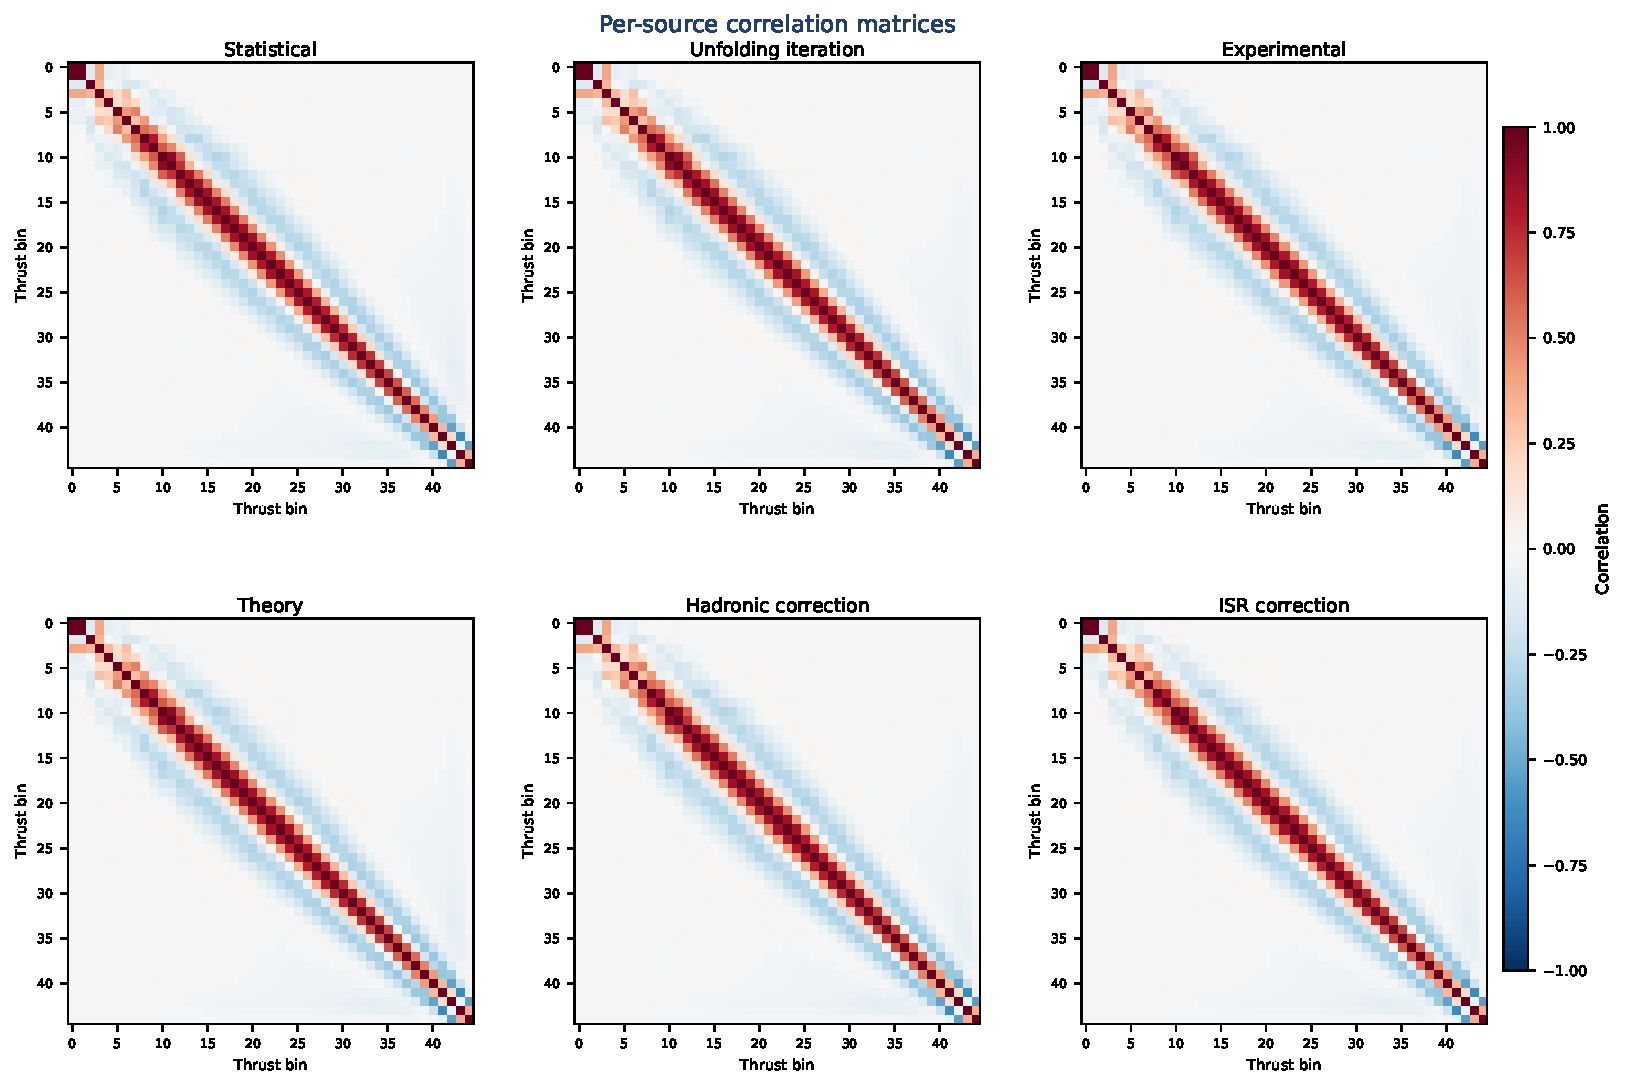
\includegraphics[width=\textwidth]{figures/corr_matrices_per_source.pdf}
\caption{Per-source correlation matrices for the six independent uncertainty
components: statistical (top left), unfolding-iteration (top center), experimental
(top right), theory (bottom left), hadronic correction (bottom center), and ISR
correction (bottom right). All matrices use the same color scale ($-1$ to $+1$,
red/blue). Under the nominal model the theory panel is diagonal (the identity), since
the theory uncertainty is a bin-wise generator envelope; the extended off-diagonal
structure resides in the statistical, iteration, and experimental panels and originates
from the unfolding of detector-level migration.}
\label{fig:corr_matrices_per_source}
\end{figure}

\FloatBarrier

\subsection{Per-source covariance matrices}
\label{sec:covariance_matrix}

The covariance matrices encode both the per-bin uncertainty magnitudes and the
bin-to-bin correlations for each source. The total covariance is the sum of all
six component covariances:
\begin{equation}
\mathrm{Cov}^{(\mathrm{tot})}_{ij} =
  \mathrm{Cov}^{(\mathrm{stat})}_{ij}
+ \mathrm{Cov}^{(\mathrm{iter})}_{ij}
+ \mathrm{Cov}^{(\mathrm{exp})}_{ij}
+ \mathrm{Cov}^{(\mathrm{theory})}_{ij}
+ \mathrm{Cov}^{(\mathrm{had})}_{ij}
+ \mathrm{Cov}^{(\mathrm{ISR})}_{ij}.
\end{equation}
Figure~\ref{fig:cov_matrices_per_source} shows the per-component covariance matrices;
Fig.~\ref{fig:cov_matrix_total} shows the total.

The component covariance magnitudes directly reflect the per-bin uncertainty sizes
shown in the breakdown plots of Sec.~\ref{sec:uncertainty_breakdown}. The theory
covariance (bottom left in Fig.~\ref{fig:cov_matrices_per_source}) has the largest
diagonal magnitude, reflecting the dominant theory envelope, but is diagonal by
construction under the nominal model and so has no off-diagonal structure. The most
extended off-diagonal structure is carried by the experimental covariance, whose
non-trivial off-diagonal entries are driven by the coherent neutral-response variations.
The statistical and iteration covariances are comparatively small; the ISR correction
produces a near-diagonal covariance consistent with its bin-local MC-statistical origin.

\begin{figure}[t!]
\centering
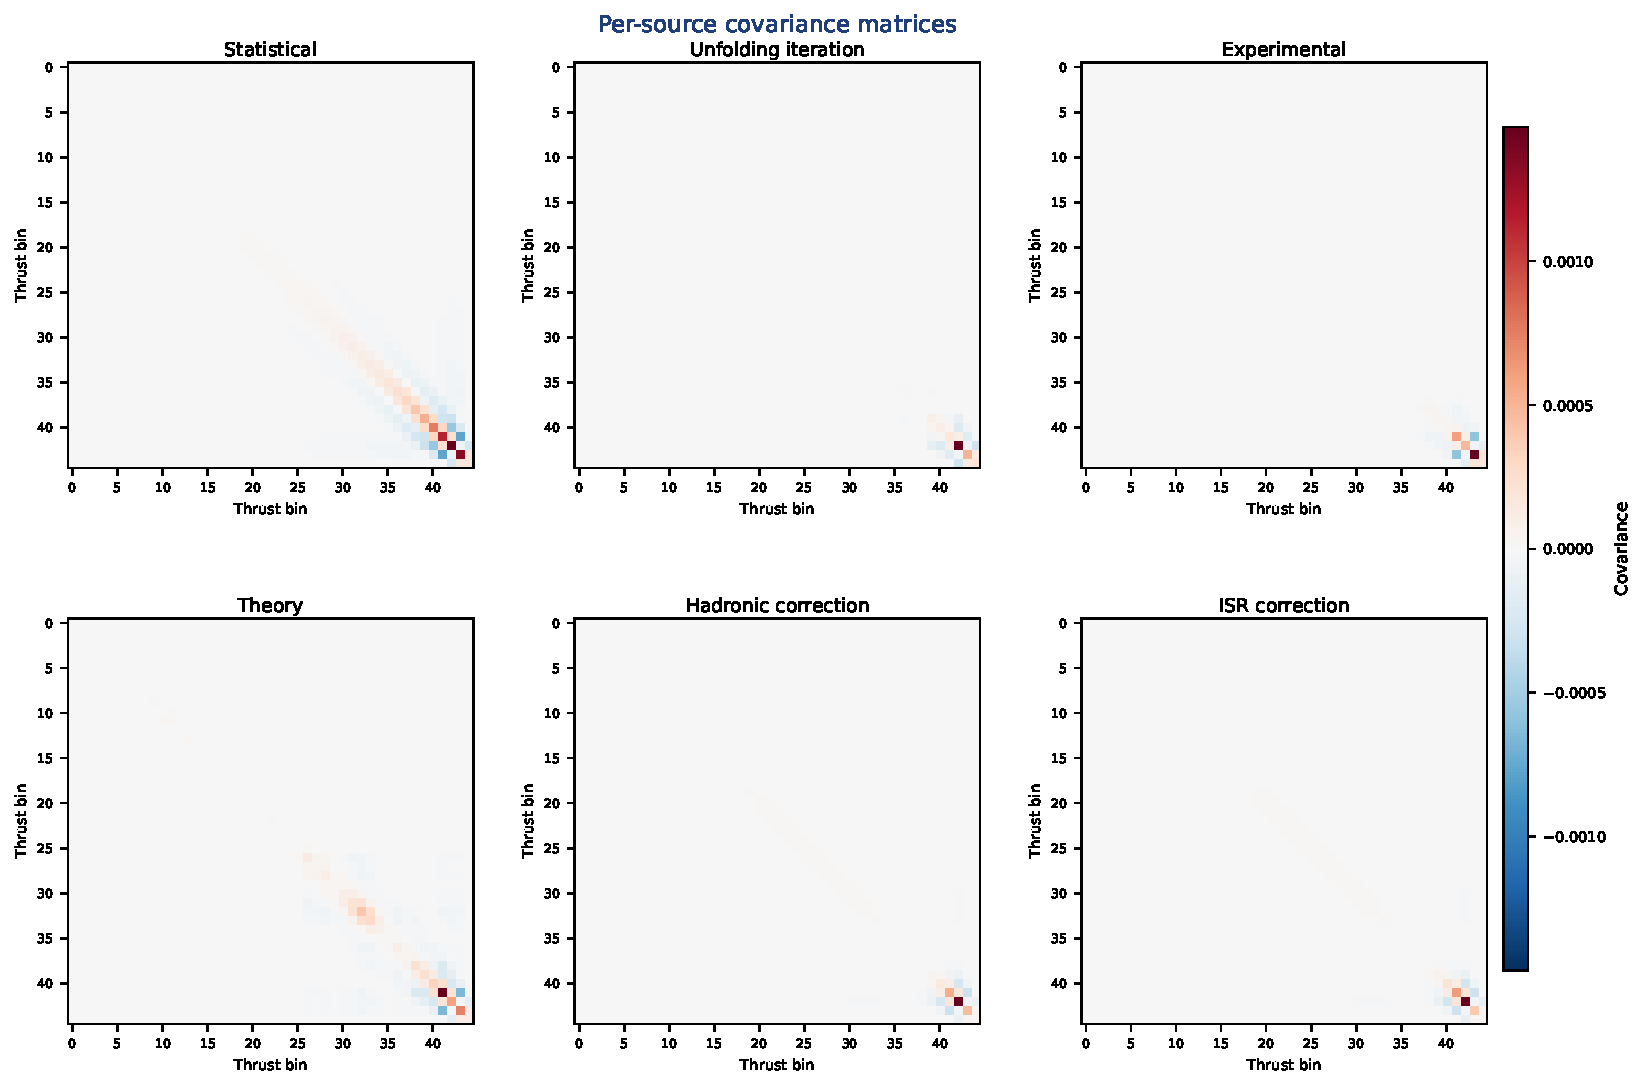
\includegraphics[width=\textwidth]{figures/cov_matrices_per_source.pdf}
\caption{Per-source covariance matrices for the six independent uncertainty
components: statistical (top left), unfolding-iteration (top center), experimental
(top right), theory (bottom left), hadronic correction (bottom center), and ISR
correction (bottom right). Each panel uses a symmetric color scale centered on zero
(red: positive, blue: negative). The theory component dominates the total covariance
in diagonal magnitude but is diagonal by construction under the nominal model; the
off-diagonal structure is carried by the experimental and statistical/unfolding
components.}
\label{fig:cov_matrices_per_source}
\end{figure}

The total covariance matrix (Fig.~\ref{fig:cov_matrix_total}) is the primary product
exported for theory use. Theory contributes the largest diagonal magnitude across the
central thrust range but, being diagonal under the nominal model, adds no off-diagonal
structure; the off-diagonal correlations come from the unfolding/response migration
(statistical covariance and the components that inherit its template) and from the
experimental component. Theory consumers are encouraged to use the fit-window total
covariance (covering $0.505\le T<1.00$, 45 bins) for $\alpha_s$ extractions rather
than the full-range matrix, to avoid the regions of large uncertainty and poor
MC-model control near the kinematic boundaries.

\begin{figure}[t!]
\centering
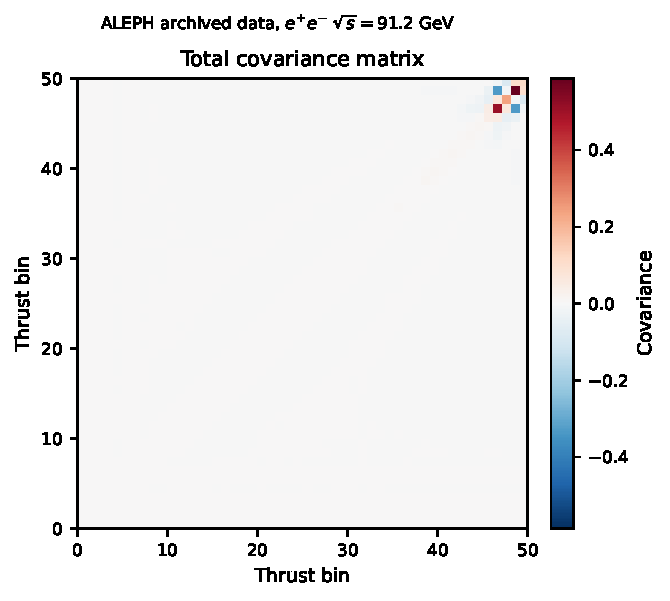
\includegraphics[width=0.72\textwidth]{figures/cov_matrix_total.pdf}
\caption{Total covariance matrix, combining all six uncertainty components.
Theory dominates the diagonal across the central thrust range but is diagonal under
the nominal model and adds no off-diagonal correlation; the off-diagonal structure
comes from the unfolding/response migration and the experimental component. The full
covariance matrix must be used in any downstream fit; diagonal uncertainties alone
would underestimate the true statistical power of the result. The fit-window version
($0.505\le T<1.00$) is recommended for $\alpha_s$ extractions.}
\label{fig:cov_matrix_total}
\end{figure}

\FloatBarrier

\section{Conclusion}
\label{sec:conclusion}

AI agents have successfully carried out a complete thrust measurement archived ALEPH 1994 data at $\sqrt{s}=91.2$~GeV under physicist guidance and collaboration. The analysis propagates uncertainty components arising from statistical, experimental, and theoretical sources and combines them in quadrature. The corresponding correlation matrices are derived from the covariance structure. The implementation of the ISR correction, following the prescription of both published ALEPH event-shape analyses~\cite{Barate:1996fi,Heister:2003aj}, brings the measured thrust distribution into good agreement with the published ALEPH 2004 result, with the only notable
discrepancy at the $T\to 1$ dijet endpoint. The AI-agent operating model demonstrated in this cycle, executable-workflow orchestration under physicist supervision with full
provenance tracking, provides a scalable framework for precision QCD as a testing ground for closed theory--experiment loops in fundamental physics.

\subsection*{Lessons from AI--Physicist Collaboration}

Carrying out this analysis has also produced practical insights into how AI agents and physicists can work together effectively. Our workflow followed a constrained human-in-the-loop cycle in which the physicist defined physics objectives, acceptance criteria, and interpretation authority, while the AI agent owned implementation and execution. Crucially, experienced physicists contribute domain context that cannot yet be reduced to formal specifications alone, including judgments about physically meaningful binning, acceptable regularization behavior, uncertainty communication, and when apparent anomalies warranted deeper investigation. A major future goal identified in this work is to translate this expert knowledge into explicit, code-based verification layers. 

From this experience, several recurring challenge classes emerged. Implicit physics priors, expert expectations about acceptable binning, regularization behavior, or uncertainty presentation, were often assumed rather than explicitly stated, requiring iterative clarification. Figure formatting and style choices (label offsets, legend placement, pad geometry) required many short feedback loops, with cosmetic shortcomings sometimes affecting interpretability and therefore physics conclusions. Synchronization across rapidly evolving scripts, outputs, and note text demanded continuous provenance refreshing. These lessons motivate creation of reusable tools, stronger configuration contracts, clearer channels for encoding expert heuristics into machine readable constraints in future iterations of this program, and new verification layers throughout the autonomous analysis flow.
% \section{Challenges with AI-agent analysis}
\label{sec:challenges}

This section is maintained as a living record of unresolved or recurring issues encountered during the analysis. Because this document is an internal note rather than a final publication, we prioritize explicit tracking of weaknesses, mitigation status, and open analysis challenges. Practical lessons from AI--physicist collaboration are discussed in Sec.~\ref{sec:context}.

\subsection{Current limitations of the thrust-only baseline}

The present release is robust enough for a preliminary thrust result, but several limitations remain:
\begin{itemize}
\item for events with exactly 3 selected particles, the thrust algorithm selects the highest-magnitude particle as the axis rather than enumerating all possible hemisphere assignments; this approximation is justified because (i) 3-particle hadronic events are rare in $Z \to q\bar{q}$ decays (impact on thrust value typically $\lesssim 0.1\%$ for $T > 0.5$), and (ii) the response-matrix migration structure dominates uncertainty in the endpoint bins where such events concentrate;
\item hadronic-event correction uncertainty is propagated as an independent component ($\Delta_{\mathrm{had}}$, central-range mean $\approx 3.2\%$); the endpoint bins remain sensitive to correction-factor extrapolation;
\item systematic inter-bin correlations use the statistical correlation matrix as a template ($\mathrm{Cov}^{(c)}_{ij} = \Delta_c(i)\,\Delta_c(j)\,\rho^{\mathrm{stat}}_{ij}$); this is an approximation that assumes systematic and statistical correlations share the same bin-to-bin structure;
\item endpoint thrust bins remain statistically and modeling sensitive;
\item analysis scope is currently one-dimensional (thrust only), while the future target includes the thrust-family observables and potentially multidimensional unfolding.
\end{itemize}

\subsection{Persistent analysis challenges}

Several recurrent issues have been tracked through the development of this analysis. Plot-style consistency across scripts has been an ongoing concern, with centralized style enforcement in producer scripts now largely resolving the issue. Method-to-code traceability gaps are addressed by the workflow and provenance tables in Sec.~\ref{sec:method} and Sec.~\ref{sec:results}, with \path{workflow_summary.json} serving as the canonical numeric record. The most significant open challenge is endpoint-bin instability: the final bin ($0.99<T<1.00$) is sensitive to MC modeling, hadronic correction extrapolation, and normalization convention differences, and dominates the maximum per-bin uncertainty. This is mitigated by reporting central-window metrics ($0.60\le T<0.95$) alongside full-range figures throughout this paper.

\subsection{Update protocol for this section}

For each major workflow iteration, this section should record:
\begin{itemize}
\item newly discovered persistent issues;
\item whether previous issues moved from Open to In progress/Resolved;
\item concrete next action and code location for unresolved items.
\end{itemize}

Keeping this log in the main body is intentional: it makes assumptions and remaining risks visible to internal readers and future maintainers.

\subsection{Scaling human oversight: toward systematic validation}
\label{sec:scaling_oversight}

A recurring theme in this work is that the set of things that can go wrong silently grows rapidly with analysis complexity. The one-dimensional thrust measurement already required validation of event selection, unfolding closure, systematic propagation, covariance-matrix properties, and figure/table accuracy. Extending the program to additional observables, multidimensional unfolding, or theory--experiment feedback loops will multiply these failure modes.

The current mitigation relies on structured sign-off points, automated integrity checks (file presence, covariance positive semi-definiteness, fit-mask validity), and version-controlled provenance. While adequate for a single-observable proof of concept, this approach does not scale without further investment in systematic testing infrastructure.

Software engineering and machine-learning operations (MLOps) communities have partially addressed analogous challenges through continuous-integration and continuous-deployment (CI/CD) pipelines, where automated test suites run on every code change and failures block deployment. Adapting these patterns to physics analysis workflows is a natural next step: for example, automated regression tests could verify that modifying one systematic variation does not silently shift the unfolded spectrum outside a predefined tolerance. Physics-specific assertions --- such as verifying that the unfolded distribution integrates to unity, that the response matrix is properly normalized, or that refolded spectra agree with detector-level data --- could be encoded as unit tests that run after each agent iteration.

The key unsolved challenge is encoding implicit physics priors as testable assertions. Many of the validation checks performed by the physicist in this analysis (Sec.~\ref{sec:ai_agent}) rely on domain intuition that is difficult to formalize: recognizing that a $\varphi$ excess indicates a detector artifact, judging whether a per-bin uncertainty is ``physically reasonable,'' or deciding that a $23\%$ shift constitutes an observable redefinition rather than a systematic effect. Developing methods to translate such expert knowledge into machine-executable tests --- whether through formal specification languages, learned anomaly detectors, or structured physicist--agent dialogue protocols --- is an important direction for making AI-assisted experimental physics robust and scalable.


\FloatBarrier
\section*{Acknowledgments}

% ALEPH
The authors would like to thank Roberto Tenchini and Guenther Dissertori from the ALEPH Collaboration for their useful comments and suggestions on the use of ALEPH data.
%
We thank all the members of the Electron-Positron Alliance for their tremendous efforts to resurrect the LEP dataset, ultimately enabling the studies presented in this paper.
% Vanderbilt
Y.C. and J.Z. are supported in part by the U.S. National Science Foundation under ID 2514008.
%
H.X.Z. is supported by the National Natural Science Foundation of China under contract No.~12425505.
% UIC
A. Baty is supported by the U.S. Department of Energy, Grant No. DE-FG02-94ER40865.
% MIT group grant
H.B., G-M. I., C.M., Y-C.C., and Y-J.L. are supported by the U.S. Department of Energy, Office of Science, Office of Nuclear Physics under grant Contract Number DE-SC0011088.
%UChi
A. Badea is supported by the Schmidt Sciences Foundation and Enrico Fermi Institute.

\bibliographystyle{JHEP}
\bibliography{biblio}

% \appendix
% \section{Workflow code and reproduction contract}
\label{sec:app_workflow_code}

This appendix documents the executable workflow structure, command sequences, and
pseudocode for the thrust analysis, moved here from the main text to keep the
analysis sections focused on physics content.

\subsection{Executable workflow map}

The thrust preliminary workflow uses two entrypoints (both under
\texttt{Unfolding/scripts/}):
\begin{itemize}
\item \texttt{run\_thrust\_prelim\_workflow.py} for nominal and systematic reruns;
\item \texttt{build\_prelim\_uncertainty\_summary.py} for uncertainty assembly and
      final summaries.
\end{itemize}
Figure~\ref{fig:workflow_schematic} summarizes the executable stages and branch structure.

\begin{figure}[t!]
\centering
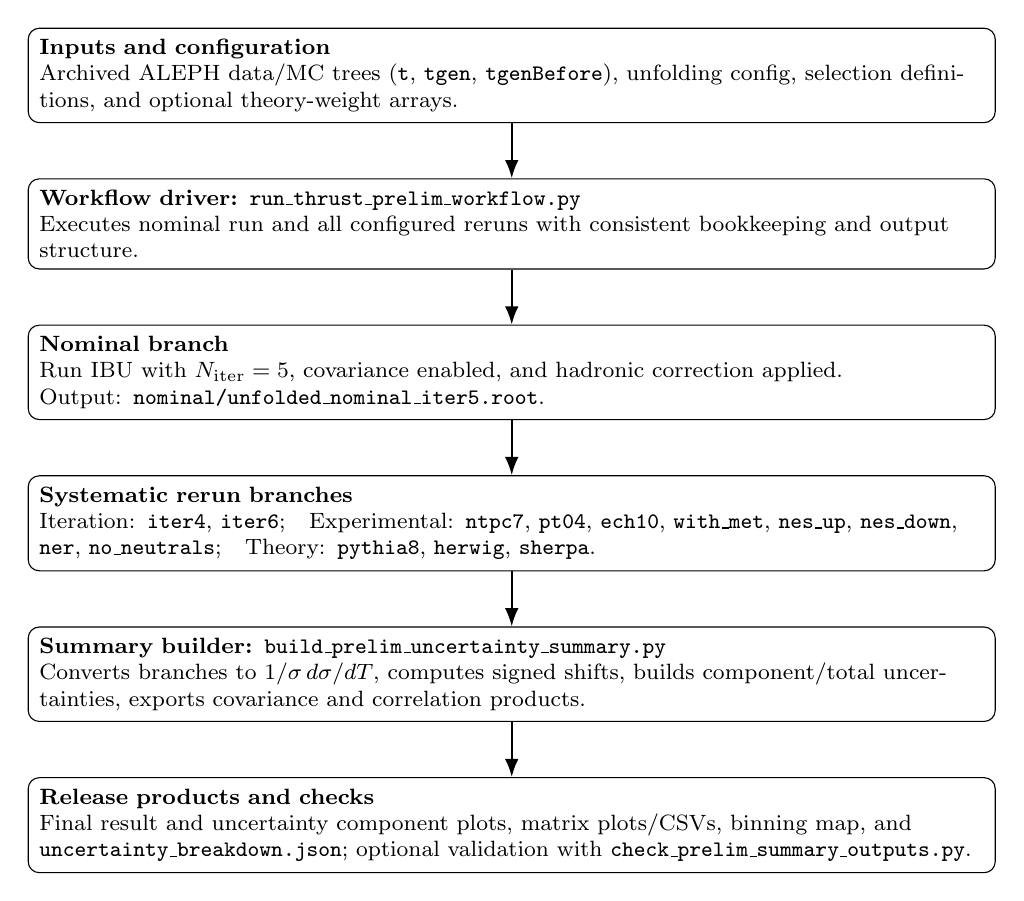
\begin{tikzpicture}[
  >=Latex,
  node distance=7mm,
  every node/.style={font=\footnotesize},
  block/.style={draw, rounded corners, align=left, text width=12.0cm, inner sep=4pt},
  arrow/.style={-Latex, line width=0.8pt}
]

\node[block] (inputs) {\textbf{Inputs and configuration}\newline
Archived ALEPH data/MC trees (\texttt{t}, \texttt{tgen}, \texttt{tgenBefore}), unfolding config, selection definitions, and optional theory-weight arrays.};

\node[block, below=of inputs] (driver) {\textbf{Workflow driver:} \texttt{run\_thrust\_prelim\_workflow.py}\newline
Executes nominal run and all configured reruns with consistent bookkeeping and output structure.};

\node[block, below=of driver] (nominal) {\textbf{Nominal branch}\newline
Run IBU with $N_{\mathrm{iter}}=5$, covariance enabled, and hadronic correction applied.\newline
Output: \texttt{nominal/unfolded\_nominal\_iter5.root}.};

\node[block, below=of nominal] (variations) {\textbf{Systematic rerun branches}\newline
Iteration: \texttt{iter4}, \texttt{iter6};\quad
Experimental: \texttt{ntpc7}, \texttt{pt04}, \texttt{ech10}, \texttt{with\_met}, \texttt{nes\_up}, \texttt{nes\_down}, \texttt{ner}, \texttt{no\_neutrals};\quad
Theory: \texttt{pythia8}, \texttt{herwig}, \texttt{sherpa}.};

\node[block, below=of variations] (summary) {\textbf{Summary builder:} \texttt{build\_prelim\_uncertainty\_summary.py}\newline
Converts branches to $1/\sigma\,d\sigma/dT$, computes signed shifts, builds component/total uncertainties, exports covariance and correlation products.};

\node[block, below=of summary] (products) {\textbf{Release products and checks}\newline
Final result and uncertainty component plots, matrix plots/CSVs, binning map, and \texttt{uncertainty\_breakdown.json}; optional validation with \texttt{check\_prelim\_summary\_outputs.py}.};

\draw[arrow] (inputs) -- (driver);
\draw[arrow] (driver) -- (nominal);
\draw[arrow] (nominal) -- (variations);
\draw[arrow] (variations) -- (summary);
\draw[arrow] (summary) -- (products);

\end{tikzpicture}
\caption{Schematic analysis flow for the thrust preliminary workflow. This replaces the dense workflow table and shows the execution order and branch structure used in this analysis.}
\label{fig:workflow_schematic}
\end{figure}


\subsection{Reproduction contract}

The following command sequence is the explicit rerun contract for this work.
It assumes a ROOT-enabled Python environment and shell access to ROOT libraries.

\begin{verbatim}
# Example environment setup
source ~/code/root/bin/thisroot.sh
conda activate py312
RUN_DIR=Studies/PreliminaryResult/2026-02-17_thrust_iter5
NOM_ROOT=$RUN_DIR/nominal/unfolded_nominal_iter5.root
SUM_DIR=$RUN_DIR/summary
MATRIX_SCRIPT=Studies/UnfoldingIterationScan/scripts/make_unfolding_matrix_plots.py

# 1) Full workflow (nominal + iteration + experimental + theory)
python Unfolding/scripts/run_thrust_prelim_workflow.py \
  --config Unfolding/unfold_config.json \
  --outdir $RUN_DIR \
  --nominal-iter 5 --iter-down 4 --iter-up 6 \
  --theory-weights-dir /path/to/theory_reweighting/training-<tag>

# 2) Uncertainty summary and final result plots
python Unfolding/scripts/build_prelim_uncertainty_summary.py \
  --base-dir $RUN_DIR \
  --outdir $SUM_DIR \
  --aleph-csv /path/to/HEPData-ins636645-v1-Table_54.csv

# 3) Matrix plots and CSV exports
python $MATRIX_SCRIPT \
  --input-root $NOM_ROOT \
  --outdir $SUM_DIR/matrices_nominal_iter5

# 4) Output integrity check
python Unfolding/scripts/check_prelim_summary_outputs.py \
  --base-dir $RUN_DIR
\end{verbatim}

The \texttt{--theory-weights-dir} argument is required unless theory variations are
explicitly skipped. If the ALEPH CSV is not available at the repository-local default
location, \texttt{--aleph-csv} must be provided explicitly.

\subsection{Workflow pseudocode}

Nominal and systematics execution logic is summarized below.

\begin{verbatim}
load nominal configuration
run nominal unfolding (iterations=5, covariance=true)
run iteration variations (iterations=4,6)
run experimental variations (ntpc7, pt04, ech10, with_met,
                             nes_up, nes_down, ner, no_neutrals)
run theory variations with event-level weights (pythia8, herwig, sherpa)
build uncertainty summary products and final plots
export covariance/correlation CSVs and matrix visualizations
validate required outputs and consistency checks
\end{verbatim}

Uncertainty-summary logic:
\begin{verbatim}
convert all unfolded branches to 1/sigma dsigma/dT
compute signed branch shifts delta_v = (U_v - U_nom)/U_nom
build components:
  iteration = envelope(iter4, iter6)
  track/event = quadrature(ntpc7, pt04, ech10, with_met)
  neutral = quadrature(envelope(nes_up, nes_down), ner)
  theory = envelope(pythia8, herwig, sherpa)
  hadronic = envelope(up/down C_had uncertainty)
build component covariance model (nominal: template_correlated)
combine total = stat + iteration + experimental + theory + hadronic
write component plots and final comparison plot
write covariance/correlation outputs over the reported bins
\end{verbatim}

\section{Validation and cross-check details}
\label{sec:app_validation}

This appendix collects supplementary validation material that supports the analysis decisions described in the main text.

\subsection{Iteration-scan closure and stability}

The iteration-scan diagnostics used to select $N_{\mathrm{iter}}=5$ confirm that the refolded spectra reproduce the detector-level data shape within the expected level of statistical fluctuation. The closure-shape $\chi^2/\mathrm{ndf}$ is stable across $N_\mathrm{iter}\in\{4,5,6\}$, and the iteration-to-iteration shift in the unfolded spectrum decreases monotonically before flattening near $N_\mathrm{iter}=5$--$6$, consistent with convergence. The $N_\mathrm{iter}=100$ refolding confirms that the response model does not diverge at high iteration, though the unfolded spectrum in that limit becomes increasingly sensitive to statistical fluctuations.

\subsection{OmniFold and prior IBU comparison}

The comparison with OmniFold~\cite{Andreassen:2019cjw} and prior Iterative Bayesian Unfolding spectra from \texttt{unfold-ee-logtau/Results} is documented in Sec.~\ref{sec:results} (Fig.~\ref{fig:final_thrust_result}). Differences are localized to the high-thrust endpoint and are consistent with the expected sensitivity of IBU to regularization strength and normalization convention in that region.

\subsection{Difference-check program}

A structured diagnostic program for inter-analysis differences (binning/normalization alignment, hadronic-correction treatment, event/sample synchronization, regularization dependence, and theory-envelope masking) is documented in \path{Plans/2026-02-19_thrust_difference_checks.md}. Execution and acceptance criteria are defined there; no final physics interpretation of residual inter-analysis differences is assigned until that program is completed.

\subsection{Output integrity verification}

After each full workflow run, a dedicated script \texttt{check\_prelim\_summary\_outputs.py} verifies that all required output files are present and non-empty, that the covariance matrix is positive semi-definite on the diagonal, and that the fit mask selects a non-zero number of bins. The 2026-03-05 run passed all checks (1/1 integrity check passed).

% \section{Communication summary (reconstructed project-cycle transcript)}
\label{sec:app_communication_summary}

This appendix records a reconstructed full communication summary for the current thrust-analysis cycle.
The source material is the project artifact trail (plans, note rewrites, workflow outputs, and validation products), not a verbatim message log.
The objective is to preserve the decision chain for internal reproducibility and method auditing.

\subsection{Scope and reconstruction sources}

Scope covered: the thrust Iterative Bayesian Unfolding cycle from code review through preliminary-result packaging and note rewrites (Sections 1--8), including the AI-agent collaboration framing.

Primary reconstruction sources:
\begin{itemize}
\item dated planning artifacts under \texttt{Plans/} (2026-02-13 to 2026-02-18);
\item executable workflow outputs in \texttt{Studies/PreliminaryResult/}, with run directory \texttt{2026-03-05\_thrust\_iter5/};
\item note section revision trail in \texttt{AnalysisNote/sections/*.tex};
\item workflow scripts in \texttt{Unfolding/scripts/} and \texttt{Studies/*/scripts/}.
\end{itemize}

\subsection{Reconstructed communication timeline}

\begin{enumerate}
\item \textbf{Initial objective setting (2026-02-13).} The collaboration established a thrust-first execution strategy with Iterative Bayesian Unfolding, complete code review, and a JHEP-style internal-note structure.
\item \textbf{Code-audit phase.} Critical and high-impact defects were identified and fixed (tree defaults, closure mode requirements, return-code handling, systematics path robustness), with findings tracked in \texttt{Plans/2026-02-13\_code\_review\_findings.md}.
\item \textbf{1994 workflow focus.} Execution direction was corrected to run the full 1994 derivation and unfolding chain rather than legacy partial-year paths.
\item \textbf{Nominal-regularization policy convergence.} The cycle converged on nominal $N_{\mathrm{iter}}=5$ with 4/6 as regularization systematic envelope for this thrust preliminary pass.
\item \textbf{Systematics completion requirement.} The scope was expanded to include full experimental and theory branches in the same run-owned output package, with hadronic correction retained in nominal processing.
\item \textbf{Result-style iteration loop.} Multiple rounds of visual QA enforced consistent pad geometry, ratio-panel readability, uncertainty normalization conventions, and legend/text placement for publication-grade interpretation.
\item \textbf{ALEPH comparison integration.} Final-result plotting was upgraded to include ratio to ALEPH 2004 in matched binning with uncertainty propagation via ROOT histogram operations.
\item \textbf{Uncertainty decomposition policy.} The workflow migrated from envelope-only views to explicit component-level plots, including signed shifts, grouped uncertainty structure, and central-window interpretation.
\item \textbf{Section-by-section rewrite cycle (Sections 1--5 first).} The note was expanded with stronger physics motivation, detector/data context, and reconstruction validation text connected directly to thrust sensitivity.
\item \textbf{Sections 5+ hardening.} Methods, systematics, and results sections were restructured for executable traceability (script entrypoints, output paths, and release artifacts).
\item \textbf{AI-agent narrative formalization.} A dedicated section captured operating model, controls, and measurable scorecard, followed by a final chapter logging persistent collaboration and analysis challenges.
\item \textbf{Physics-tone refinement.}\\
Introductory framing was strengthened around precision-QCD motivation,\\
LEP data quality, and validation goals.
\item \textbf{External-citation expansion.}\\
AI-for-science and agent-workflow references were expanded, then extended with requested recent case studies.
\item \textbf{Reproducibility emphasis.} The communication repeatedly enforced path-level provenance for figures and summary products, with explicit checks and output validation scripts.
\item \textbf{Current-cycle layout request.} Results narrative was requested to present uncertainty decomposition before the final unfolded comparison, and to add a final-result total correlation matrix view.
\item \textbf{Current-cycle documentation request.} A complete communication appendix was requested for community context, with highlighted key decisions and rationale.
\end{enumerate}

\subsection{Key exchanges and decisions}

\newcommand{\decisionbox}[3]{%
\noindent\fbox{%
\parbox{0.97\textwidth}{%
\textbf{Decision:} #1\\
\textbf{Rationale:} #2\\
\textbf{Impact:} #3
}}%
}

\decisionbox
{Use Iterative Bayesian Unfolding as the baseline correction method for this cycle.}
{Fast iteration without model retraining was required for rapid experimental cross-check loops.}
{Workflow scripts, method text, and uncertainty propagation were all aligned to IBU.}

\decisionbox
{Set nominal regularization to $N_{\mathrm{iter}}=5$ with 4/6 as regularization systematic.}
{Iteration-scan diagnostics and practical stability/throughput tradeoffs favored this operating point.}
{All nominal and systematic branches, note text, and final plots were normalized to the same policy.}

\decisionbox
{Run the full 1994 chain as the maintained baseline dataset year.}
{The analysis state required consistency in data/MC derivation and response inputs for one complete production year.}
{Output provenance and note references were consolidated under run-owned 1994 directories.}

\decisionbox
{Adopt a strict figure-style contract for result plots (connected pads, controlled ratio range, readable labels).}
{Visual interpretation quality was treated as analysis-relevant, not cosmetic.}
{Several plotting scripts were iteratively corrected until style and uncertainty semantics stabilized.}

\decisionbox
{Promote component-level uncertainty views (statistical, unfolding, experimental, theory) over envelope-only summaries.}
{Readers need source-resolved behavior rather than only combined envelopes.}
{Results section now reports component behavior explicitly and ties interpretation to central-window metrics.}

\decisionbox
{Keep ``no-neutrals'' as a cross-check branch and separate it from nominal total uncertainty.}
{It is a stress test rather than a baseline uncertainty source.}
{Cross-check visibility is preserved while nominal total remains policy-consistent.}

\decisionbox
{Introduce explicit AI-agent operating-model and challenge-tracking sections.}
{The internal-note objective includes evaluating whether an agent can execute research workflows under supervision.}
{The note now contains controls, measurable scorecard, and persistent challenge logging.}

\decisionbox
{Expand citations to include recent AI+scientist and theory-assistant case studies.}
{Program motivation required concrete external evidence beyond generic AI discussion.}
{Introduction and AI-agent sections now cite both broad and recent workflow-relevant studies.}

\decisionbox
{Reorder results narrative to show uncertainty structure before final unfolded comparison.}
{Interpretation of the final spectrum is clearer once uncertainty sources are established first.}
{Section flow now progresses from component structure to correlated final products to central comparison.}

\decisionbox
{Add a final-result total correlation matrix plot from \texttt{corr\_total.csv}.}
{Community-facing usage requires direct visibility of correlated uncertainties after full nominal combination.}
{Release package now includes a dedicated final total-correlation figure and script-level provenance.}

\subsection{Communication-pattern summary}

The reconstructed cycle indicates a high-frequency specification--execution loop with strong emphasis on:
\begin{itemize}
\item explicit physics-policy locking before broader text expansion;
\item figure-level interpretability as a first-class requirement;
\item command/path-level provenance for every released artifact;
\item incremental correction and revalidation rather than large unreviewed batches.
\end{itemize}

The dominant friction points were precision formatting constraints, rapid scope evolution, and synchronization between code outputs and note narrative. These patterns are consistent with the persistent-challenge tracker in Sec.~\ref{sec:challenges}.


\end{document}
